% !TEX root = Fernanda.tex

% !TEX root = Fernanda.tex

%% abtex2-modelo-trabalho-academico.tex, v-1.9.6 laurocesar
%% Copyright 2012-2016 by abnTeX2 group at http://www.abntex.net.br/ 
%%
%% This work may be distributed and/or modified under the
%% conditions of the LaTeX Project Public License, either version 1.3
%% of this license or (at your option) any later version.
%% The latest version of this license is in
%%   http://www.latex-project.org/lppl.txt
%% and version 1.3 or later is part of all distributions of LaTeX
%% version 2005/12/01 or later.
% -------------------------------------------------------------------------------
% -------------------------------------------------------------------------------
% abnTeX2: Modelo de dissertaçao para o mestrado-PROFMAT) 
% em conformidade com ABNT NBR 14724:2011,ABNT NBR 6027:2012,
%
%  Preparado por Rigoberto G.S. Castro - Professor do LCMAT-CCT-UENF (09/08/2017)
% -------------------------------------------------------------------------------
% -------------------------------------------------------------------------------

\documentclass[
	% -- opções da classe memoir --
	12pt,				% tamanho da fonte
	openright,			% capítulos começam em pág ímpar (insere página vazia caso preciso)
	%twoside,			% para impressão em verso e anverso. Oposto a oneside
	oneside,           	% para impressão  apenas verso
	a4paper,			% tamanho do papel. 
	% -- opções da classe abntex2 --
	%chapter=TITLE,		% títulos de capítulos convertidos em letras maiúsculas
	%section=TITLE,		% títulos de seções convertidos em letras maiúsculas
	%subsection=TITLE,	% títulos de subseções convertidos em letras maiúsculas
	%subsubsection=TITLE,% títulos de subsubseções convertidos em letras maiúsculas
	% -- opções do pacote babel --
	english,			% idioma adicional para hifenização
	%	french,				% idioma adicional para hifenização
	%	spanish,			% idioma adicional para hifenização
	brazil				% o último idioma é o principal do documento
]{abntex2}

% ---
% Pacotes básicos 
% ---

%----
% Pacote fonte, Usa a fonte Arial Exigencia UENF para Posgraduacao
% ---	
%\usepackage[scaled]{uarial}     %
\usepackage{tgheros}
\renewcommand*\familydefault{\sfdefault} %% Only if the base font of the document is to be sans serif
% ---
%\usepackage{lmodern}			% Usa a fonte Latin Modern, Padrao para outras universidades		
\usepackage[T1]{fontenc}		% Selecao de codigos de fonte.
\usepackage[utf8]{inputenc}		% Codificacao do documento (conversão automática dos acentos)
\usepackage{lastpage}			% Usado pela Ficha catalográfica
\usepackage{indentfirst}		% Indenta o primeiro parágrafo de cada seção.
\usepackage{color}				% Controle das cores
\usepackage{graphicx}			% Inclusão de gráficos
\usepackage{subfig}             % Inclusão de gráficos (subfloat)
\usepackage{subcaption}         % subfiguras
% Comentei o próximo pacote, porque ele dá bug com o abntex2 --- Rafael
% \usepackage{microtype} 			% para melhorias de justificação
\usepackage{amsmath,amssymb,amsfonts,amsthm,textcomp} % Pacotes de Matemática
\usepackage{pdfpages}           % Para incluir arquivos pdf
\usepackage{verbatim}
\usepackage{booktabs}
\usepackage{multirow}
% ---
% Pacotes adicionais, usados apenas no âmbito do Modelo Canônico do abnteX2
% ---

\usepackage{lipsum}				% para geração de dummy text
% ---
% Pacotes de citações
% ---
\usepackage[brazilian,hyperpageref]{backref}	 % Paginas com as citações na bibl
\usepackage[alf]{abntex2cite}	% Citações padrão ABNT
\graphicspath{{Pictures/}{Imagens/}{Figuras/}}



\setlength{\parindent}{1.3cm} % --- Espaçamentos entre linhas e parágrafos --- %
\setlength{\parskip}{0.2cm}  % Controle do espaçamento entre um parágrafo e outro/tente também \onelineskip


%\selectlanguage{english} % Seleciona o idioma do documento (conforme pacotes do babel)
\selectlanguage{brazil} % Seleciona o idioma do documento (conforme pacotes do babel)


\frenchspacing % Retira espaço extra obsoleto entre as frases.

\makeindex % --- compila o índice ---


% === ALTERAÇÕES ALINE ===

\newcommand{\eps}{\varepsilon}
\newcommand{\red}[1]{{\color{red} #1}}
\newcommand{\green}[1]{{\color{OliveGreen} #1}}
\newcommand{\blue}[1]{{\color{blue} #1}}

\newcommand{\couple}[2]{(#1, \, #2)}
\newcommand{\triple}[3]{(#1, \, #2, \, #3)}
\newcommand{\quadruple}[4]{(#1, \, #2, \, #3, \, #4)}
\newcommand{\interval}[2]{[#1, \, #2]}
\newcommand{\vetord}[2]{\left\langle #1, \, #2 \right\rangle}
\newcommand{\vetort}[3]{\left\langle #1, \, #2, \, #3 \right\rangle}

\newcommand{\naturais}{\mathbb{N}}
\newcommand{\inteiros}{\mathbb{Z}}
\newcommand{\racionais}{\mathbb{Q}}
\newcommand{\reais}{\mathbb{R}}
\newcommand{\algebricos}{\mathbb{A}}
\newcommand{\partes}[1]{\mathcal{P}(#1)}
\newcommand{\interior}[1]{{#1}^{\mathrm{o}}}
\newcommand{\fecho}[1]{\overline{#1}}

\newcommand{\intdef}[4]{\displaystyle \int_{#3}^{#4} #1 \, d#2}
\newcommand{\intind}[2]{\displaystyle \int #1 \, d#2}
\newcommand{\calculado}[3]{{#1} \Big|_{#2}^{#3}}
\newcommand{\LHo}{\overset{\mathrm{\text{L'Hô}}}{=}}
\newcommand{\despr}{\overset{\mathrm{\text{despr.}}}{=}}
\newcommand{\portanto}{\quad \therefore \quad}

\DeclareMathOperator{\sen}{sen}
\DeclareMathOperator{\tg}{tg}
\DeclareMathOperator{\cotg}{cotg}
\DeclareMathOperator{\senh}{senh}
\DeclareMathOperator{\tgh}{tgh}
\DeclareMathOperator{\cotgh}{cotgh}
\DeclareMathOperator{\sech}{sech}
\DeclareMathOperator{\cossech}{cossech}
\DeclareMathOperator{\arctg}{arctg}
\DeclareMathOperator{\arcsen}{arcsen}
\DeclareMathOperator{\arccotg}{arccotg}
\DeclareMathOperator{\arcsec}{arcsec}
\DeclareMathOperator{\arccossec}{arccossec}
\DeclareMathOperator{\arcsenh}{arcsenh}
\DeclareMathOperator{\arccosh}{arccosh}
\DeclareMathOperator{\arctgh}{arctgh}
\DeclareMathOperator{\arccotgh}{arccotgh}
\DeclareMathOperator{\arcsech}{arcsech}
\DeclareMathOperator{\arccossech}{arccossech}
\DeclareMathOperator{\sinal}{sinal}

\newcommand{\tq}{\,\,|\,\,}
\DeclareMathOperator{\Dom}{Dom}
\DeclareMathOperator{\Ima}{Im}
\DeclareMathOperator{\Gra}{Gra}
\DeclareMathOperator{\Laplace}{\mathcal{L}}

\renewcommand{\sin}{\sen}
\renewcommand{\sinh}{\senh}
\renewcommand{\tan}{\tg}
\renewcommand{\tanh}{\tgh}

\newcommand{\edsreta}[1]{\draw[->,thick] (-5,0)--(5,0) node[right]{$#1$}}
\newcommand{\edsraiz}[1]{plot[only marks,thin,mark=+,mark size=3pt] coordinates{(#1,0)}}
\newcommand{\edssing}[1]{plot[only marks,thin,mark=x,mark size=4pt] coordinates{(#1,0)}}
\newcommand{\edslegenda}[2]{(#1,0) node[below]{$#2$}}
\newcommand{\edssinal}[2]{(#1,0) node[above]{$#2$}}

\newcommand{\ext}{^\wedge}
\DeclareMathOperator{\rot}{rot}

%\newtheorem{exemplo}{Exemplo}
%\newtheorem*{exemplo*}{Exemplo}
%\newtheorem*{notacao}{Notação}
%\newtheorem*{pergunta}{Pergunta}
%\newtheorem*{definicao}{Definição}
%\newtheorem*{observacao}{Observação}
%\newtheorem{teorema}{Teorema}
%\newtheorem*{demonstracao}{Demonstração}
%\newtheorem{propriedade}{Propriedade}
% !TEX root = Fernanda.tex

\setlength{\marginparwidth}{2cm}

\usepackage{todonotes}
\usepackage{etoolbox}
\usepackage{soul}

%%%%% Comandos de TODO
%%% Cores pessoais. Acrescentem as suas
\definecolor{Rafael}{HTML}{00B7EB}
\definecolor{Joel}{HTML}{2700EC}
\definecolor{Nelson}{HTML}{00FF04}
\definecolor{Oscar}{HTML}{FF9A00}
\definecolor{Monique}{HTML}{FF00A7}

%%% Não mexer aqui
\let\oldtodo\todo
%\renewcommand{\todo}[2]{\oldtodo[inline,color=#1]{\textbf{TODO} [#1]: #2}}
\renewrobustcmd{\todo}[2]{\sethlcolor{#1}\hl{[#1]: #2}\addcontentsline{tdo}{todo}{[#1]: #2}}

\newcommand{\coment}[2]{\oldtodo[color=#1]{#1: #2}}

\newcommand{\acrescentar}[1]{\textcolor{red}{#1}\addcontentsline{tdo}{todo}{Texto acrescentado}}

\newcommand{\substituir}[2]{\st{#1}\textcolor{red}{#2}\addcontentsline{tdo}{todo}{Texto substituído}}

\newcommand{\remover}[1]{\st{#1}\addcontentsline{tdo}{todo}{Texto removido}}

\newcommand{\marcatexto}[1]{\sethlcolor{yellow}\hl{#1}\addcontentsline{tdo}{todo}{Texto marcado}}

\DeclareRobustCommand{\atualizar}[1]{\sethlcolor{yellow}\hl{\textit{#1}}\addcontentsline{tdo}{todo}{Atualizar texto}}

\newcommand{\missingtable}[1]{\sethlcolor{orange}\begin{tabular}{|c|c|c|} \hline \hl{Fazer tabela} & \hl{Fazer tabela} & \hl{Fazer tabela} \\ \hline \hl{Fazer tabela} & \hl{Fazer tabela} & \hl{Fazer tabela} \\ \hline \hl{Fazer tabela} & \hl{Fazer tabela} & \hl{Fazer tabela} \\ \hline \end{tabular}\addcontentsline{tdo}{todo}{Table: #1}}

% --- 
% CONFIGURAÇÕES DE PACOTES
% --- 

% ---
% Configuracoes para inserir e listar QUADROS
% para atender às regras da ABNT
% ---
\newcommand{\quadroname}{Quadro}
\newcommand{\listofquadrosname}{Lista de quadros}

\newfloat[chapter]{quadro}{loq}{\quadroname}
\newlistof{listofquadros}{loq}{\listofquadrosname}
\newlistentry{quadro}{loq}{0}
%
\counterwithout{quadro}{chapter}
\renewcommand{\cftquadroname}{\quadroname\space}
\renewcommand*{\cftquadroaftersnum}{\hfill--\hfill}


% ---
% Configuracoes para inserir e listar Gráficos
% para atender às regras da ABNT
% ---
\newcommand{\graficoname}{Gráfico}
\newcommand{\listofgraficosname}{Lista de gráficos}

\newfloat[chapter]{grafico}{logg}{\graficoname}
\newlistof{listofgraficos}{logg}{\listofgraficosname}
\newlistentry{grafico}{logg}{0}
%
\counterwithout{grafico}{chapter}
\renewcommand{\cftgraficoname}{\graficoname\space}
\renewcommand*{\cftgraficoaftersnum}{\hfill--\hfill}

%
% ---
% Configurações do pacote backref
% Usado sem a opção hyperpageref de backref
%---
\renewcommand{\backrefpagesname}{Citado na(s) página(s):~}
% Texto padrão antes do número das páginas
\renewcommand{\backref}{}
% Define os textos da citação
\renewcommand*{\backrefalt}[4]{
	\ifcase #1 %
		Nenhuma citação no texto.%
	\or
		Citado na página #2.%
	\else
		Citado #1 vezes nas páginas #2.%
	\fi}%
% ---

% ---
%Configuracao Usado para Modificar titulo dos capitulos modelo UENF
%---

\renewcommand{\ABNTEXchapterfont}{\fontfamily{cmr}\fontseries{b}\selectfont}
\renewcommand{\ABNTEXchapterfontsize}{\HUGE}
%\chapterstyle{ger}
\chapterstyle{default}
%---

%---
% Definicoes de ambientes
%--
\newtheorem{definicao}{Definição}[chapter]
\newtheorem{teorema}{Teorema}[chapter]
\newtheorem{lema}{Lema}[chapter]
\newtheorem{obs}{\small Observa\c c\~ao}[chapter]
\newtheorem{exemplo}{\small Exemplo}[chapter]


%--
%---
%   DEFINICOES ESPECIAIS PARA USAR EM FORMULAS MATEMATICAS
%---
\DeclareMathOperator*{\supess}{\sup\,ess}
\DeclareMathOperator*{\di}{div}
\DeclareMathOperator*{\dd}{d_e}
%\DeclareMathOperator*{\sen}{sen}
\DeclareMathOperator*{\dis}{d}
\DeclareMathOperator*{\linear}{linear}
\DeclareMathOperator*{\e}{e}
%\DeclareMathOperator*{\arcsen}{arcsen}
\DeclareMathOperator*{\juta}{bruna}
\newcommand{\somatorio}{\displaystyle\sum_{j=1}^{m}}
\newcommand{\un}{\mathbf{u}}
\newcommand{\x}{\mathbf{x}}
\newcommand{\phin}{\boldsymbol{\phi}}
\newcommand{\is}{\boldsymbol{\Big(}}%Producto interno
\newcommand{\de}{\boldsymbol{\Big)}}%Producto interno
\newcommand{\C}{\mathbb{C}}
\newcommand{\RN}{\mathbb{R}^{n}}
\newcommand{\Rt}{\mathbb{R}^{3}}
\newcommand{\Rd}{\mathbb{R}^{2}}
\newcommand{\R}{\mathbb{R}}
\newcommand{\N}{\mathbb{N}}
\newcommand{\Z}{\mathbb{Z}}

% \newenvironment{demonstracao}{  \noindent{ \textbf{\small Demonstra\c c\~ao}}:  }

% ---

% === ALTERAÇÕES FERNANDA ===
\def\legendaTabela{Fonte: Elaboração própria}
\def\autoria{Fonte: Acervo da Pesquisa}

% \usepackage{subcaption}
\usepackage{graphicx}
\usepackage{caption}
% \captionsetup{font=small, labelfont=bf}
% \captionsetup[sub]{labelsep=period, subrefformat=brace}

% Figuras automaticamente centralizadas com fonte
\newenvironment{CenteredFigure}{\begin{figure}[htbp]\centering}{\end{figure}}
\newenvironment{MyCenteredFigure}{\begin{CenteredFigure}}{\legend{\autoria}\end{CenteredFigure}}

\newenvironment{CenteredTable}{\begin{table}[htbp]\centering}{\end{table}} % Centered Tables



% --- Informações de dados para CAPA e FOLHA DE ROSTO --- %

\autor{\textbf{Fernanda Maria da Silva Fernandes}}
\titulo{Uso da Metodologia Resolução de Problemas No Ensino-Aprendizagem-Avaliação de Geometria Espacial - Poliedros}
% \local{Campos dos Goytacazes, RJ, Brasil}
\local{UNIVERSIDADE ESTADUAL DO NORTE FLUMINENSE\\
  DARCY RIBEIRO - UENF\\
  CAMPOS DOS GOYTACAZES - RJ}
\data{\today}

\def\orientadorTCC{Profª. Drª. Elba Orocia Bravo Asenjo}


\preambulo{``Dissertação apresentada ao Centro de Ciência e Tecnologia da Universidade Estadual do Norte Fluminense Darcy Ribeiro, como parte das exigências para obtenção do título de Mestre em Matemática.''}

\orientador{\orientadorTCC}

% \instituicao{}

\tipotrabalho{Dissertação de Mestrado}

% --- Configurações de aparência do PDF final

\definecolor{blue}{RGB}{41,5,195} % alterando o aspecto da cor azul

% informações do PDF
\makeatletter
\hypersetup{
  %pagebackref=true,
  pdftitle={\@title},
  pdfauthor={\@author},
  pdfsubject={\imprimirpreambulo},
  pdfcreator={LaTeX with abnTeX2},
  pdfkeywords={abnt}{latex}{abntex}{abntex2}{trabalho acadêmico},
  colorlinks=true,      % false: boxed links; true: colored links
  linkcolor=blue,       % color of internal links
  citecolor=blue,       % color of links to bibliography
  filecolor=magenta,    % color of file links
  urlcolor=blue,
  bookmarksdepth=4
}
\makeatother
% --- 


\begin{document} % --- Início do documento ---

\pretextual{} % --- INÍCIO DOS ELEMENTOS PRÉ-TEXTUAIS ---

\imprimircapa{} % Capa
\imprimirfolhaderosto{} % Folha de rosto (o * indica que haverá a ficha bibliográfica)

% Ficha catalográfica

% 
% ---
% Inserir a ficha bibliografica
% ---
%     NA UENF ESTA FICHA É FEITO PELO BIBLIOTECARIO
% ---

% Isto é um exemplo de Ficha Catalográfica, ou ``Dados internacionais de
% catalogação-na-publicação''. Você pode utilizar este modelo como referência. 
% Porém, provavelmente a biblioteca da sua universidade lhe fornecerá um PDF
% com a ficha catalográfica definitiva após a defesa do trabalho. Quando estiver
% com o documento, salve-o como PDF no diretório do seu projeto e substitua todo
% o conteúdo de implementação deste arquivo pelo comando abaixo:
%
\begin{fichacatalografica}
	%     \includepdf{fig_ficha_catalografica.pdf}
\end{fichacatalografica}
%
%  Nao usado a ficha catalografica
%
\begin{comment}
\begin{fichacatalografica}
	\sffamily
	\vspace*{\fill}					% Posição vertical
	\begin{center}					% Minipage Centralizado
		\fbox{\begin{minipage}[c][8cm]{13.5cm}		% Largura
				\small
				\imprimirautor
				%Sobrenome, Nome do autor

				\hspace{0.5cm} \imprimirtitulo  / \imprimirautor. --
				\imprimirlocal, \imprimirdata-

				\hspace{0.5cm} \pageref{LastPage} p. : il. (algumas color.) ; 30 cm.\\

				\hspace{0.5cm} \imprimirorientadorRotulo~\imprimirorientador\\

				\hspace{0.5cm}
				\parbox[t]{\textwidth}{\imprimirtipotrabalho~--~\imprimirinstituicao,
					\imprimirdata.}\\

				\hspace{0.5cm}
				1. Palavra-chave1.
				2. Palavra-chave2.
				2. Palavra-chave3.
				I. Orientador.
				II. Universidade xxx.
				III. Faculdade de xxx.
				IV. Título
			\end{minipage}}
	\end{center}
\end{fichacatalografica}
\end{comment}
% ---
 % Utilizado?
% 
% ---
% Inserir errata - Opcional
% ---
\begin{comment}
\begin{errata}
Elemento opcional da \citeonline[4.2.1.2]{NBR14724:2011}. Exemplo:

\vspace{\onelineskip}

FERRIGNO, C. R. A. \textbf{Tratamento de neoplasias ósseas apendiculares com
reimplantação de enxerto ósseo autólogo autoclavado associado ao plasma
rico em plaquetas}: estudo crítico na cirurgia de preservação de membro em
cães. 2011. 128 f. Tese (Livre-Docência) - Faculdade de Medicina Veterinária e
Zootecnia, Universidade de São Paulo, São Paulo, 2011.

\begin{table}[htb]
\center
\footnotesize
\begin{tabular}{|p{1.4cm}|p{1cm}|p{3cm}|p{3cm}|}
\hline
\textbf{Folha} & \textbf{Linha}  & \textbf{Onde se lê}  & \textbf{Leia-se}  \\
\hline
1 & 10 & auto-conclavo & autoconclavo\\
\hline
\end{tabular}
\end{table}
\end{errata}
\end{comment}
% --- % Não utilizado

% --- Inserir folha de aprovação --- %

% Isto é um exemplo de Folha de aprovação, elemento obrigatório da NBR
% 14724/2011 (seção 4.2.1.3). Você pode utilizar este modelo até a aprovação
% do trabalho. Após isso, substitua todo o conteúdo deste arquivo por uma
% imagem da página assinada pela banca com o comando abaixo:

%\includepdf{folhadeaprovacao_final.jpg}

% \begin{comment}

\begin{folhadeaprovacao}

  \begin{center}
    {\ABNTEXchapterfont\large\imprimirautor}

    \vspace*{\fill}\vspace*{\fill}
    {\ABNTEXchapterfont\bfseries\Large\imprimirtitulo}
    \vspace*{\fill}

    \hspace{.45\textwidth}
    \begin{minipage}{.5\textwidth}
      \imprimirpreambulo
    \end{minipage}%
    \vspace*{\fill}
  \end{center}

  %   Trabalho aprovado. \imprimirlocal, 24 de setembro de 2024:

  \assinatura{\textbf{Prof. Roger Ruben Huaman Huanca}\\ D. Sc. - UEPB}
  \assinatura{\textbf{Prof. Ausberto Silverio Castro Vera}\\ D. Sc. - UENF}
  \assinatura{\textbf{Prof. Luis Humberto Guillermo Felipe}\\ D. Sc. - UENF}
  \assinatura{\textbf{Elba Orocia Bravo Asenjo} \\ D. Sc. - UENF\\ (ORIENTADORA)}

  % \begin{center}
  %   \vspace*{0.5cm}
  %   {\large\imprimirlocal}
  %   \par
  %   {\large\imprimirdata}
  %   \vspace*{1cm}
  % \end{center}

\end{folhadeaprovacao}
% \end{comment}


% ---
% Dedicatória
% ---
\begin{dedicatoria}
	\vspace*{\fill}
	\centering
	\noindent
	\begin{flushright}
		\begin{minipage}{10cm}
			\emph{Dedico esta dissertação a Deus, pela força e orientação em todos os momentos desta jornada, ao meu marido Antônio Carlos, à minha tia Francy, aos meus filhos João Vítor e Daniel.
				Aos meus alunos, que ao longo desses anos de magistério, me ensinaram muito mais do que eu pude ensinar a eles.}
		\end{minipage}
	\end{flushright}
	\vspace{3cm}
\end{dedicatoria}


% ---
% Agradecimentos
% ---
\begin{agradecimentos}
  Agradeço a Deus, pela força, sabedoria e orientação em todos os momentos desta jornada.

  Ao meu querido marido, por seu amor incondicional, paciência e apoio constante, que me incentivaram a seguir em frente mesmo nos momentos mais desafiadores.

  Aos meus filhos, que são a fonte de minha inspiração e alegria diária. Seu carinho e compreensão me motivaram a nunca desistir dos meus sonhos.

  À minha tia, pelo encorajamento, pelos conselhos sábios e por sempre acreditar em mim. Sua presença em minha vida é um presente inestimável.

  Aos meus colegas de turma, agradeço profundamente pelo apoio mútuo e pela força que compartilhamos ao longo dessa jornada. Juntos, enfrentamos e superamos muitas dificuldades, e essa solidariedade foi fundamental para o nosso sucesso.

  A todos vocês, meu mais profundo agradecimento e amor eterno.

\end{agradecimentos}

% \begin{comment}
% ---
% Epígrafe
% ---
\begin{epigrafe}
	\vspace*{\fill}
	\begin{flushright}
		\textit{``Mestre não é quem sempre ensina,\\
			mas quem de repente aprende.''\\
			João Guimarães Rosa}
	\end{flushright}
	\vspace{3cm}
\end{epigrafe}
% ---
% \end{comment}


% resumo em português
\setlength{\absparsep}{18pt} % ajusta o espaçamento dos parágrafos do resumo
\begin{resumo}
    % A metodologia ativa de resolução de problemas é uma abordagem educacional que coloca os alunos no centro do processo de aprendizagem, incentivando-os a resolver problemas do mundo real por meio da aplicação de conhecimentos e habilidades. Esta metodologia é particularmente eficaz pois promove a participação ativa, o pensamento crítico, a criatividade e a colaboração. A pesquisa busca responder se essa metodologia constitui um caminho alternativo eficaz para a construção de conceitos geométricos espaciais. Os objetivos incluem desenvolver habilidades de resolução de problemas, compreensão profunda de conceitos geométricos, aplicação prática da geometria, desenvolvimento de competências transversais e aumento do engajamento e motivação dos alunos. Os professores atuam como facilitadores, guiando os alunos através de atividades práticas e colaborativas, como estudos de caso, simulações, projetos de grupo, debates e experiências práticas. A metodologia inclui etapas como identificação do problema, contextualização, exploração, colaboração, experimentação, reflexão e apresentação. A dissertação está organizada em capítulos que abordam a introdução, referencial teórico, aspectos metodológicos, desenvolvimento das atividades didáticas e considerações finais.

    % A metodologia ativa de resolução de problemas é uma abordagem educacional que coloca os alunos no centro do processo de aprendizagem, incentivando-os a resolver problemas do mundo real por meio da aplicação de conhecimentos e habilidades. Neste trabalho, propõe-se a aplicação dessa metodologia para a construção do aprendizado sobre conceitos geométricos espaciais com alunos do ensino médio. Para tanto, o professor atua como facilitador, elaborando atividades que promovam a participação ativa, o pensamento crítico, a criatividade e a colaboração dos alunos. Nessas aulas especialmente desenvolvidas, segue-se uma sequência de dez etapas que incluem a leitura do problema, coletiva, solução do problema pelos docentes acompanhados pelo docente e posteriormente apresentados aos demais alunos com os quais as resoluções eram discutidas para que a turma alcançasse um consenso, por fim formalizando o conteúdo abordado. Com a aplicação dessa metodologia, foi identificado elevada taxa de participação dos alunos, e um aumento significativo no engajamento e motivação dos discentes. Além disso, através do feedback dado pelos alunos, demonstra-se a satisfação dos mesmos com a metodologia aplicada. Diante do exposto, conclui-se que a metodologia ativa de resolução de problemas é uma abordagem eficaz para a construção de conceitos geométricos espaciais, visto que promove o engajamento e motivação nos alunos, bem como os auxilia a fixar o conteúdo de forma mais eficaz.

    Percebe-se que, no ensino da Geometria Espacial, muitos alunos apresentam dificuldades em compreender conceitos abstratos, como os relacionados aos poliedros, e em aplicá-los em contextos práticos. A abordagem tradicional, muitas vezes focada na memorização de fórmulas e procedimentos, não parece promover uma compreensão profunda e significativa dos conteúdos. Assim sendo, propomo-nos no presente trabalho verificar se o uso da Metodologia de Ensino-Aprendizagem-Avaliação de Matemática através da Resolução de Problemas constitui-se num caminho alternativo para a construção de conceitos e conteúdos geométricos espaciais pelos alunos do Ensino Médio. Trata-se de uma abordagem educacional que coloca o aluno no centro do processo de aprendizagem, incentivando-o a ser um aprendiz ativo e autônomo. Nesse método, os alunos aprendem através da resolução de problemas reais ou simulados, em vez de simplesmente receber informações passivamente. Esta abordagem foi aplicada a estudantes da 2º série do ensino médio da escola pública. Ao final desta pesquisa conseguimos demonstrar que a resolução de problemas é um dos principais métodos para ensinar, aprender e avaliar a Matemática em sala de aula. Com base nas evidências coletadas nesta pesquisa, acreditamos fortemente que a Metodologia de Ensino-Aprendizagem-Avaliação de Matemática através da Resolução de Problemas é uma alternativa eficaz que permite aos alunos a construção de conceitos e conteúdos matemáticos, explorando e aproveitando seu próprio potencial e habilidades. Os alunos ficaram comprometidos com o trabalho e focados nas atividades propostas, não havendo dispersão. Conseguimos também, uma evolução significativa dos rendimentos qualitativos e quantitativos. Diante dos resultados é possível concluir que a Metodologia Resolução de Problemas se torna, assim, um recurso valioso não só para ensinar, mas também para aprender e praticar Matemática. Assim, futuras pesquisas podem expandir o conhecimento sobre a metodologia de resolução de problemas, explorando sua aplicação em diferentes contextos e conteúdos, desenvolvendo novos recursos didáticos, focando na formação de professores e comparando-a com outras abordagens inovadoras.

    \textbf{Palavras-chave}:  Metodologia Resolução de Problemas; Geometria Espacial; Poliedros.

\end{resumo}


% resumo em inglês
\begin{resumo}[Abstract]
	\begin{otherlanguage*}{english}
		 The main objective of this dissertation is to verify the effectiveness of the Methodology of Teaching-Learning-Assessment of Mathematics through Problem Solving in the construction of concepts and contents of Spatial Geometry - Polyhedrons by high school students. In the context of Mathematics Education, this methodology is seen as an active and alternative approach, centered on the student, where problems that generate new mathematical concepts and contents are used to promote the construction of knowledge. In this approach, students actively participate in the construction of knowledge under the guidance and supervision of the teacher, who formalizes the ideas constructed only at the end of the process, using correct notation and terminology. The thematic units worked on were the introduction of spatial geometry, Euler's relation and polyhedrons. The results demonstrated that the use of this methodology increased the motivation of both teachers and students and allowed students to relate their activities to previously studied topics, promoting a more meaningful and integrated learning.
		
		\vspace{\onelineskip}
		
		\noindent
		\textbf{Key-words}: Teaching-Learning-Assessment Methodology; Problem Solving; Spatial Geometry; Polyhedrons; Euler's Relation; Knowledge Construction; Active Methodology; Student Motivation.
	\end{otherlanguage*}
\end{resumo}

% ---
% inserir lista de ilustrações
% ---
\pdfbookmark[0]{\listfigurename}{lof}
\listoffigures*
\cleardoublepage
% ---

% --- inserir lista de tabelas ---

\pdfbookmark[0]{\listtablename}{lot}
\listoftables*
\cleardoublepage


% ---
% inserir o sumario
% ---
\pdfbookmark[0]{\contentsname}{toc}
\tableofcontents*
\cleardoublepage
% ---


\textual{} % --- INÍCIO DOS ELEMENTOS TEXTUAIS ---

\chapter{Introdução} \label{cap:1_introducao}

Uma das principais características do ser humano é a tendência de evitar conflitos. No entanto, no cotidiano, somos frequentemente confrontados com situações desafiadoras, e é nesse contexto que a educação desempenha um papel crucial, nos preparando e desenvolvendo habilidades para resolvê-las. Ao ensinar por meio do método de Resolução de Problemas, o foco do aprendizado é transferido para o aluno, enquanto o professor assume o papel de orientador. Isso permite que o aluno seja um participante ativo, em vez de passivo, como no ensino mecânico, promovendo sua autonomia e preparando-o para enfrentar a vida real.

Portanto, a Resolução de Problemas no ensino da Matemática possibilita ao aluno desenvolver capacidades intelectuais, como o pensamento matemático, o senso crítico e a autonomia. Para que isso ocorra, é essencial que a resolução de problemas não seja trabalhada de forma isolada dos conteúdos, mas sim como uma ferramenta para a construção dos conceitos, onde novas informações são integradas ao conhecimento prévio. Dessa forma, o aluno tem a oportunidade de vivenciar situações reais na sala de aula, facilitando a descoberta de novas ideias.

% Este trabalho está estruturado da seguinte forma: na Introdução, são apresentadas a justificativa, a pergunta norteadora, o objetivo geral e os objetivos específicos, que visam demonstrar o interesse pelo tema e esclarecer a finalidade da pesquisa. Em seguida, o Referencial Teórico oferece embasamento para a análise dos dados. A Metodologia descreve o tipo de pesquisa, os instrumentos utilizados e os participantes. Posteriormente, os Resultados e Discussão apresentam e analisam os dados coletados. O trabalho é finalizado com as Considerações Finais, as Referências e o Apêndice.

A aprendizagem matemática tem sido um componente essencial no desenvolvimento cognitivo dos alunos, fornecendo ferramentas fundamentais para o raciocínio lógico, a resolução de problemas e a tomada de decisões. O estudo dos conceitos matemáticos segue uma progressão estruturada, partindo de ideias simples e concretas até alcançar tópicos mais abstratos e complexos. Esse processo ajuda os estudantes a construir uma base sólida de conhecimento, permitindo a aplicação de princípios matemáticos em situações práticas e no cotidiano. O desenvolvimento dessas habilidades também estimula a autonomia intelectual e a capacidade de pensar criticamente sobre problemas diversos.

% Apesar de sua relevância, a aprendizagem matemática, quando limitada a abordagens repetitivas e mecânicas, pode não explorar todo o potencial criativo e investigativo dos estudantes. A prática excessiva de exercícios com foco apenas na memorização de fórmulas ou na aplicação direta de algoritmos pode dificultar o desenvolvimento de um entendimento mais profundo e crítico da matemática. Por isso, é essencial incorporar metodologias ativas, como a resolução de problemas, exploração de situações reais e investigação matemática, que envolvem os alunos em processos de aprendizagem mais dinâmicos e interativos, permitindo uma experiência mais rica e significativa no aprendizado.

\section{Problemática}

Apoiados na ideia e no desejo de poder motivar alunos e professores diante de situações envolvendo a Geometria Espacial, a pergunta que a pesquisa pretende responder ao final desta aplicação e avaliação de resultados é: A aplicação da Metodologia de Ensino-Aprendizagem-Avaliação de Matemática através da Resolução de Problemas representa uma alternativa para a construção de conceitos e conteúdos geométricos espaciais pelos alunos do Ensino Médio?

\section{Objetivos}

Objetivo Geral:

Investigar a eficácia da Metodologia de Resolução de Problemas no Ensino-Aprendizagem-Avaliação da Geometria Espacial, analisando seu impacto na compreensão conceitual dos alunos e no desenvolvimento de habilidades práticas e críticas.

Objetivos Específicos:

\begin{enumerate}
    % \item Desenvolver a capacidade dos alunos de compreender a fórmula de Euler $(V - A + F = 2)$ para poliedros convexos e aplicá-la corretamente;
    % \item Ensinar o que é a área lateral de um poliedro (a soma das áreas de todas as faces laterais) e como ela difere da área total;
    % \item Ensinar que a área total de um poliedro é a soma da área lateral e da área das bases;
    % \item Ensinar o conceito de volume como a quantidade de espaço ocupado por um poliedro;
    % \item Capacitar os alunos a calcular o volume de cubos, prismas, pirâmides e outros poliedros, utilizando as fórmulas apropriadas;
    % \item Desenvolver a capacidade de construção e representação de figuras geométricas;
    % \item Compreender os passos para se resolver um problema;
    % \item Selecionar problemas geradores de novos conceitos geométricos;
    % \item Utilizar uma metodologia diferente da tradicional para trabalhar a Geometria Espacial;
    % \item Trabalhar problemas interdisciplinares que apresentem o conteúdo de forma contextualizada;
    % \item Verificar se a metodologia utilizada promove a aprendizagem de novos conceitos.

    % \item Desenvolver a capacidade dos alunos de compreender a fórmula de Euler $(V - A + F = 2)$  para poliedros convexos e aplicá-la corretamente;
    % \item Desenvolver a capacidade de construção e representação de figuras geométricas;
    % \item Compreender os passos para se resolver um problema;
    % \item Selecionar problemas geradores de novos conceitos geométricos;
    % \item Utilizar uma metodologia diferente da tradicional para trabalhar a Geometria Espacial;
    % \item Trabalhar problemas interdisciplinares que apresentem o conteúdo de forma contextualizada;
    % \item Capacitar os alunos a calcular área lateral, área total e volume dos poliedros, utilizando as fórmulas apropriadas;
    % \item Verificar se a metodologia utilizada promove a aprendizagem de novos conceitos.

    % \item Fazer uma pesquisa bibliográfica sobre os aspectos básicos relacionados com a Metodologia Resolução de Problemas;
    % \item Compreender as etapas indicadas na Metodologia, para resolver um determinado problema;
    % \item Compreender o conceito de Problema Gerador de novos conceitos matemáticos;
    % \item Selecionar um conjunto de problemas básicos de Geometria Espacial - Poliedros e treinar os alunos na aplicação da Metodologia;
    % \item Aplicar a Metodologia Resolução de Problemas utilizando os problemas selecionados;
    % \item Trabalhar problemas interdisciplinares que apresentem o conteúdo de forma contextualizada;
    % \item Desenvolver a capacidade de construção e representação de figuras geométricas;
    % \item Elaborar uma análise dos resultados obtidos, a partir da aplicação da Metodologia, em sala de aula.

    \item Realizar uma pesquisa bibliográfica sobre os aspectos fundamentais da Metodologia de Resolução de Problemas, além de compreender o conceito de Problema Gerador de novos conceitos matemáticos;
    \item Entender as etapas recomendadas pela Metodologia para resolver problemas específicos e selecionar um conjunto de problemas básicos de Geometria Espacial - Poliedros;
    \item Aplicar a Metodologia de Resolução de Problemas utilizando os problemas selecionados e elaborar uma análise dos resultados obtidos em sala de aula;
    \item Trabalhar com problemas interdisciplinares que apresentem o conteúdo de forma contextualizada;
    \item Desenvolver a capacidade de construção e representação de figuras geométricas.

\end{enumerate}

\section{Justificativa}

O que motivou o desenvolvimento desta pesquisa foi a percepção de que, no ensino da Geometria Espacial, muitos alunos apresentam dificuldades em compreender conceitos abstratos, como os relacionados aos poliedros, e em aplicá-los em contextos práticos. A abordagem tradicional, muitas vezes focada na memorização de fórmulas e procedimentos, não parece promover uma compreensão profunda e significativa dos conteúdos. Assim, sentiu-se a necessidade de investigar formas de engajar os alunos mais ativamente e desenvolver suas capacidades de pensamento crítico e resolução de problemas.

A escolha da Metodologia de Resolução de Problemas como foco central desta pesquisa se deu pela sua capacidade de colocar o aluno no centro do processo de aprendizagem, promovendo a construção do conhecimento de maneira mais participativa e reflexiva. E como, a partir dela pode-se agregar também metodologias ativas, como Gamificação, Sala de Aula Invertida, dentre outras, acredita-se que essa abordagem oferece uma forma mais eficiente de ensino, em que os alunos podem aplicar os conceitos de Geometria Espacial em situações concretas, desenvolvendo não apenas habilidades matemáticas, mas também sua autonomia intelectual.

A motivação, portanto, surge da vontade de contribuir para a melhoria da aprendizagem de Geometria Espacial, explorando formas de ensino que proporcionem um aprendizado mais profundo e significativo, ao mesmo tempo em que capacitem os alunos para enfrentar problemas reais de maneira criativa e eficaz.

\section{Estrutura da Dissertação}

O texto do trabalho está organizado da seguinte forma: no \autoref{cap:1_introducao} inicia-se com a apresentação da introdução, na qual são destacadas a motivação para o trabalho e considerações da pesquisadora, os objetivos geral e específicos da pesquisa; no \autoref{cap:2_referencial} discute-se o referencial teórico que deu suporte e balizou essa pesquisa; no \autoref{cap:3_aspectos}, descreve-se o percurso metodológico utilizado nessa pesquisa; no \autoref{cap:4_aplicacao}, destacamos o desenvolvimento das atividades da sequência didática; e por fim no \autoref{cap:5_consideracoes}, as considerações finais.

% --- CAPITULOS ---

% --- PARTE DESENVOLVIMENTO ---
% Parte principal do texto, que contém a exposição ordenada e pormenorizada do assunto. Divide-se capítulos, seções e subseções, que variam em função da abordagem do tema e do método. Pode ter: Revisão Bibliográfica, Material e Métodos, Resultados, Discussão

\chapter{Referencial Teórico} \label{cap:2_referencial}

Neste Capítulo apresenta-se uma breve revisão sobre Metodologias Ativas, tipos de Metodologias Ativas e a Metodologia Resolução de Problemas.

A Base Nacional Comum Curricular (BNCC) defende a aplicação dos conhecimentos na vida real, a importância do contexto para dar sentido ao que se aprende e o protagonismo do estudante, tanto em sua aprendizagem como na construção de seu projeto de vida. As escolas são o espaço onde as crianças se desenvolvem diariamente, aprendendo sobre si mesmas e ao se relacionar com o próximo. Os alunos aprendem, desde seus primeiros anos, muito mais do que os conteúdos ensinados pelos educadores. Ao referirmos sobre o aluno nos deparamos com a aprendizagem e o protagonismo e percebemos que há uma ligação entre os três; é impossível falarmos de uma só, pois os mesmos estão fortemente ligados pela Base \cite[p. 2]{FRANCESCONI2019}.

\begin{citacao}
    Os seis direitos de aprendizagem e desenvolvimento asseguram, na educação, as condições para que as crianças aprendam em situações nas quais possam desempenhar papel ativo em ambientes que as convidem a vivenciar desafios e a sentirem-se provocadas a resolvê-los, nas quais possam construir significados sobre si, os outros e o mundo social e natural \cite[p. 35]{EducacaoSecretariadeEducacaoFundamental2017}.
\end{citacao}

Assim, segundo \citeonline{NOGUEIRA2020} os choques entre as deficiências no ensino atual, tem sido relatada como falta de protagonismo dos estudantes emanadas pelos modelos de educação tradicional.

Diante do cenário educacional na atualidade, com o avanço das Tecnologias Digitais e a efetivação das redes sociais na rotina diária dos estudantes tem-se agravado a realidade das salas de aula, nas quais o desinteresse pelos conteúdos trabalhados tem se tornado cada vez mais evidente. Uma das consequências dessa nova realidade é que a sala de aula, tornou-se um ambiente repetitivo, ambiente que não desperta a vontade por aprender. Todavia tornou-se imprescindível alterar a dinâmica da aula e a forma de ensinar, e as metodologias ativas é um meio de proporcionar essa mudança. No entanto, é necessário retomar o significado das teorias e as possibilidades rotineiras passando ao desenvolvimento da uma prática pedagógica que consiste em metodologias ativas capazes de promover um aprendizado mais prazeroso e eficiente \cite[p. 2]{DUMONT2016}.

Visando fortalecer essa discussão, \citeonline[p. 277-278]{DIESEL2017} afirmam que ``para superar esse modelo, é preciso valorizar a inovação em sala de aula, renovando metodologias, inventando metodologias ou criando metodologias. Assim, a metodologia ativa de ensino exige, tanto do professor quanto do estudante, a ousadia para inovar no âmbito educacional''.

Em face disso, \citeonline[p. 5]{Segura2015} esclarecem que ``um aspecto importante desenvolvido pelo estudante nesta concepção de ensino diz respeito à autonomia. Aprender a ser autônomo favorece o amadurecimento do estudante no mundo acadêmico, mas em muitas vezes gera o desconforto nos primeiros passos''.

Nesse sentido, o estudo de \citeonline{CARDOSO2019} conclui que o uso de Metodologias Ativas se mostrou eficaz para as interações entre professor, aluno e conteúdo.  Apresentou resultados favoráveis ao uso de metodologias capazes de evidenciar o cotidiano dos alunos, que passaram a se posicionar de forma mais efetiva nos debates.

Analogamente, \citeonline{CARVALHO2021} detalham que aprendizagem ativa ocorre quando o aluno interage com o assunto, ouvindo, falando, fazendo e ensinando. E, desta forma, o aluno é estimulado a construir o conhecimento ao invés de ser apenas um receptor. Uma das possibilidades de envolvimento dos alunos utilizadas pelos autores foi a construção de jogos educativos pelos quais observaram que os alunos se sentiram desafiados a buscar conhecimento para a elaboração do mesmo e a praticar para poder vencer as etapas do jogo.

Segundo os autores, o ensino por meio de jogos possibilita a criação de um ambiente motivador que é necessário para a maximização de potenciais, o que facilita a dinâmica do processamento cognitivo de informações  \cite{CARVALHO2021}, ``ampliação progressiva da capacidade de abstração e da autonomia de ação e de pensamento, possibilitando ao aluno explorar aspectos mais complexos das relações consigo mesmo, com os outros e com o ambiente'' \cite[p. 295]{EducacaoSecretariadeEducacaoFundamental2017} .

\section{Trilhando pelos caminhos das Metodologias Ativas}

As metodologias ativas são abordagens de ensino que se baseiam na participação dos estudantes no processo de aprendizagem, em contraste com os métodos tradicionais de ensino, nos quais os alunos têm um papel mais passivo, de receptor das informações. Essas metodologias visam promover a melhor compreensão, o pensamento crítico, a resolução de problemas e a aplicação prática do conhecimento.

O vocábulo metodologias ativas não é novo, mas muito se tem discutido sobre sua importância e influência na educação, pois o grande desafio dos professores sempre foi encontrar e utilizar um método de como ensinar para manter ativa a participação e o envolvimento dos discentes no desenvolvimento das aulas. Assim, as metodologias ativas são estratégias de ensino que objetivam incentivar os alunos a aprenderem de forma autônoma e participativa, através de problemas e situações reais, realizando tarefas que os estimulem a pensar, a tomarem iniciativa, tornando-se responsáveis pela construção de seu próprio conhecimento \cite[p. 12]{DIESEL2017}.

Fazendo uma breve retrospectiva, é possível enfatizar que as metodologias ativas têm seu início antes da década de 1980, onde estudiosos buscavam mostrar os inúmeros fatores que interferem no processo de aprendizagem, como também identificar a necessidade de desenvolver novas habilidades capazes de despertar o desejo por aprender. Nesse sentido, as metodologias ativas defendem uma maior participação do aluno no seu próprio aprendizado sendo sujeitos ativos e participantes, onde a função dos docentes passa a ser monitor do conhecimento, tendo como papel proporcionar ambientes diversos e criativos para a aprendizagem de seus alunos \cite[p. 263]{Mota2018}.

Surgem assim as metodologias ativas como proposta para ``focar o processo de ensinar e aprender na busca da participação ativa de todos os envolvidos, centrados na realidade em que estão inseridos'' \cite[p. 66]{FIALHO2017}.

O pensamento pedagógico de \citeonline{DEWEY1979} (apud \cite{LOVATO2018} p.156-157) defende a liberdade por parte do aluno em buscar seu próprio conhecimento.

\begin{citacao}
    O objetivo da educação é visto como a formação de estudantes com competência e criatividade, capazes de gerenciar sua própria liberdade. Dewey criticou a cultura de obediência e submissão, enfatizando o seu desgosto mediante a memorização de conteúdos pelos educandos presente nas escolas, a qual para ele era na verdade um obstáculo à verdadeira educação. Ele então postulou que para o progresso da ordem social, deveriam ser buscados os princípios da iniciativa, originalidade e da cooperação.
\end{citacao}

O uso de metodologias ativas como estratégias do processo ensino e aprendizagem nos diversos eixos de estudo, podendo ser na matemática e ciências, entre outras disciplinas, precisam quebrar barreiras que impedem o aprendizado ativo e participativo dos alunos, pois é sabido que o mundo evoluiu e por isso é preciso rever as antigas práticas pedagógicas de modo a favorecer o ensino-aprendizado dos alunos.

São considerados ``métodos ativos'' aqueles que possibilitam um aprender participativo e, nesta metodologia, ``os discentes participam de aulas desafiadoras e significativas em que o professor assume o papel de mediador'' \cite[p. 56]{GOUVEIA2019}.

Para \citeonline[p. 29]{SOUSA2022} ``as Metodologias Ativas de Aprendizagem são ferramentas de ensino colaborativo centradas no aluno, em que os alunos são incentivados a participar de discussões e atividades práticas'', as metodologias ativas são compreendidas ``[...] como práticas pedagógicas alternativas ao ensino tradicional''.

As Metodologias Ativas são estratégias de aprendizagem que colocam o estudante no centro do processo de ensino, promovendo sua autonomia e participação ativa. Segundo \citeonline{MORAN2018}, essas metodologias são aplicadas para tornar o aprendizado mais significativo e envolvente, enquanto \citeonline{Santos2022} destacam que elas se baseiam na autonomia, problematização da realidade, reflexão, valorização do trabalho em equipe e inovação. O estudante, como agente construtor de seu próprio conhecimento, é incentivado a ser mais ativo e participativo, desenvolvendo uma postura crítica e coparticipativa durante o processo de ensino.

Essas metodologias também enfatizam a problematização da realidade e a reflexão, buscando uma relação constante entre teoria e prática. A fragmentação do conteúdo é evitada, e o aprendizado é contextualizado com a vida real, permitindo que os alunos critiquem e reflitam sobre a realidade, sentindo-se desafiados e curiosos sobre os problemas propostos. O trabalho em equipe é valorizado, criando um ambiente de discussão e interação social, onde as trocas de opiniões e argumentos são vistas positivamente. Além disso, a inovação é incentivada, buscando maneiras alternativas de interação entre professor e aluno, com o professor atuando como mediador, facilitador e orientador, em vez de ser apenas uma fonte de informações.

A educação contemporânea tem como premissa central a formação de indivíduos críticos, autônomos e capazes de interagir ativamente no processo de construção do conhecimento. Nesse contexto, o foco não está apenas na transmissão de conteúdos, mas na criação de um ambiente de aprendizagem que favoreça o desenvolvimento integral do estudante. A relação entre professor e aluno é transformada, promovendo maior participação, reflexão e engajamento, com metodologias que incentivam o pensamento crítico, a colaboração e a inovação. A seguir, são destacados os principais aspectos que fundamentam as metodologias ativas compilados por \citeonline[adaptado pela autora]{Santos2022}.

\begin{citacao}
    \begin{itemize}
        \item \textbf{Aluno}: o estudante é agente construtor de seu próprio conhecimento, tem controle do processo de aprendizagem, sendo guiado por atividades que permitam ser mais ativo e participativo.
        \item \textbf{Autonomia}: um aluno com controle de seu processo de aprendizagem, desenvolve sua autonomia, devido a postura crítica e coparticipativa durante o processo de ensino e da liberdade durante as aulas.
        \item \textbf{Problematização da realidade e reflexão}: há uma busca constante na relação entre teoria e prática, fugindo da fragmentação do conteúdo, e buscando a problematização da realidade, a possibilidade de significar o aprendizado a partir da contextualização com a vida, surgindo a ação do estudante em criticar e/ou refletir sobre a realidade e tomar consciência dela, de se sentir desafiado e curioso sobre os problemas propostos.
        \item \textbf{Trabalho em equipe}: as estratégias didáticas adotadas estão repletas de momentos de discussão e de interação social, refletindo na atitude do aluno e do professor, criando um ambiente em que há possibilidade de opinar e argumentar, no qual as trocas com o outro são vistas positivamente.
        \item \textbf{Inovação}: inovar é buscar maneiras alternativas de interação entre o professor e o aluno, que fujam da aula pautada na transmissão pelo professor e a absorção de conteúdos e o papel de ouvinte passivo do aluno.
        \item \textbf{Professor}: possui um papel de mediador, de facilitador, de orientador e não mais de fonte de informações e de transmissor delas.
    \end{itemize}
\end{citacao}

\begin{citacao}
    É importante destacar que as Aprendizagens Ativas possuem princípios articulados com correntes teóricas consagradas, dos quais o mais importante é o Ensino centrado no aluno, que deve ser estimulado a ter uma postura ativa, exercitando assim sua autonomia \cite[p. 33]{SOUSA2022}.
\end{citacao}

O esforço necessário para esse tipo de aprendizagem é muito menor, daí ele ser tão utilizado quando os alunos se preparam para exames escolares \cite[p. 27]{SOUSA2022}.

``As teorias que se desenvolveram em torno da aprendizagem, não se esgotam em si mesmas, tampouco uma sobrepõe a outra, mas entre elas existe uma relação de continuidade e de complementaridade'' \cite[p. 5]{LACERDA2023}.

A escolha da metodologia pode depender do contexto, dos objetivos de aprendizagem e das preferências dos educadores e dos alunos, pois conforme indica \citeonline{MASETTO2012}, ``[...] toda aprendizagem, para que realmente aconteça, precisa ser significativa para o aprendiz, isto é, precisa envolvê-lo como pessoa, como um todo: ideias, inteligência, sentimento, cultura, profissão e sociedade''.

Portanto, a escolha da metodologia ativa depende dos objetivos de aprendizagem, do contexto educacional e das necessidades dos alunos. Muitas vezes, uma combinação de abordagens ativas é usada para criar um ambiente de aprendizado dinâmico e eficaz. O objetivo principal é envolver os alunos de forma mais profunda e tornar a aprendizagem mais significativa, pois ``quando isso ocorre o aluno é induzido a refletir sobre suas ações e valores, o que pode levá-lo a mudá-los para que se estabeleça harmonia entre seus conhecimentos, valores e condutas'' \cite[p. 315]{FRASSON2019}.

O professor possui um papel de mediador, de facilitador, de orientador e não mais de fonte de informações e de transmissor delas, conforme indicado por \citeonline{Santos2022}
% (Quadro \ref{tab:Princípios das Metodologias Ativas propostas por Santos e Castaman})
, e, para tanto:

\begin{citacao}
    O profissional da área da educação, precisa desenvolver habilidades que contribuam o suficiente para a construção do conhecimento. Vale lembrar que o ambiente educacional trará as pressões externas e, ao professor cabe trabalhar com essas novas necessidades, de modo que o aluno perceba como os modos de produção e as relações de poder modificam, a fim de sempre perpetuar seu domínio \cite[p. 4]{NathBragaTeixeira2017}.
\end{citacao}

\section{Os Tipos de Metodologias Ativas na literatura}

As metodologias ativas não se restringem a um único método de aplicação, mas a variadas práticas que tem como objetivo tornar a aula mais proveitosa e dinâmica, e \citeonline{Santos2022} propõem diversos exemplos de metodologias ativas.

\begin{itemize}
    \item \textbf{Aprendizagem Baseada em Problemas (ABP)}: nessa abordagem, os alunos são apresentados a problemas complexos e tarefas que precisam ser resolvidas, eles trabalham em grupos para investigar, pesquisar e encontrar soluções para esses problemas.
    \item \textbf{Aprendizagem Baseada em Projetos}: os alunos trabalham em projetos significativos e de longo prazo que incentivam a pesquisa, planejamento e execução, podem abranger diversas disciplinas e promover a colaboração, a criatividade e a resolução de problemas.
    \item \textbf{Sala de aula invertida}: nessa abordagem, os alunos estudam o material antes da aula, muitas vezes por meio de vídeos ou leituras, e a sala de aula é usada para discussão, atividades práticas e esclarecimento de dúvidas.
    \item \textbf{Aprendizagem entre Pares ou Aprendizagem colaborativa}: a aprendizagem colaborativa envolve os alunos trabalhando em grupos para alcançar objetivos de aprendizagem. Eles compartilham conhecimentos, resolvem problemas juntos e aprendem uns com os outros, promovendo habilidades de trabalho em equipe e comunicação.
    \item \textbf{Gamificação}: a gamificação incorpora elementos de jogos na aprendizagem para torná-la mais envolvente e motivadora.
    \item \textbf{Ensino por descoberta}: nessa metodologia, os alunos são incentivados a descobrir conceitos e princípios por meio da exploração ativa, experimentação e resolução de problemas, em vez de receber informações passivamente.
    \item \textbf{Aprendizagem baseada em equipe}: os alunos trabalham em equipes para tarefas ou projetos, promovendo a realização, a comunicação e o desenvolvimento de habilidades interpessoais.
    \item \textbf{Ensino híbrido}: combina elementos do ensino presencial e online para oferecer flexibilidade e personalização na aprendizagem.
    \item \textbf{Aprendizagem auto-organizada}: os alunos têm a responsabilidade de definir seus próprios objetivos de aprendizagem, selecionar recursos e avaliar seu próprio progresso.
\end{itemize}

De acordo com \citeonline[p. 16]{MORAN2012} ``os métodos tradicionais, que privilegiam a transmissão de informações pelos professores, faziam sentido quando o acesso à informação era difícil''.

Para \citeonline{DEWEY1979}, ``os homens vivem em comunidade em virtude das coisas que têm em comum; e a comunicação é o meio porque chegam a possuir coisas comuns.'' Dessa forma, estabelecem relações com o meio social de forma a se constituírem. ``O que eles devem ter em comum para formar uma comunidade ou sociedade são os objetivos, as crenças, as aspirações, os conhecimentos, um modo comum de compreender, mentalidade similar, conforme dizem os sociólogos.'' \cite[p. 17]{DEWEY1979}.

Segundo \citeonline[p. 16]{CAMARGO2018} ``o uso de metodologias ativas de aprendizagem desenvolve competências pessoais e profissionais, além daquelas desenvolvidas na aula tradicional''. Segundo  \citeonline[p. 16]{CAMARGO2018}, ``a utilização de atividades de aprendizagem mais ativas, por meio de práticas colaborativas, melhoram o aprendizado e a capacidade de retenção do conhecimento''.

Segundo Valente ``metodologias ativas constituem alternativas pedagógicas que colocam o foco do processo de ensino e de aprendizagem no aprendiz, envolvendo-o na aprendizagem por descoberta, investigação ou resolução de problemas'' \cite[p. 27]{VALENTE2018}.

\citeonline{MORAN2012} acredita que o ``nosso desafio maior é caminhar para um ensino e uma educação de qualidade, que integrem todas as dimensões do ser humano.'' A educação de forma integral, na sua totalidade, e isso implica o envolvimento de ``pessoas que façam essa integração, em si mesmas, do sensorial, intelectual, emocional, ético e tecnológico, que transitem de forma fácil entre o pessoal e o social, que expressem nas palavras e ações que estão sempre evoluindo, mudando, avançando.'' \cite[p. 29]{MORAN2012}.

Ele completa dizendo que ``O jovem lê o que pode visualizar, precisa ver para compreender: Toda a sua fala é mais sensorial-visual do que racional e abstrata. Lê, vendo.'' \cite[p. 29]{MORAN1995}.

\citeonline{DEWEY1979} reflete sobre ``a possibilidade de compartilhar os conhecimentos adquiridos com a comunidade educativa, colegas, estudantes, famílias e a possibilidade de promover mudanças cultura que contribua com as disciplinas regulares.'' Sob uma visão integradora, perpassa o conhecimento, que ocorre entre as disciplinas ``numa perspectiva transdisciplinar, com uma formação integral, numa perspectiva dialógica e que, sobretudo, possa preparar para viver de forma mais feliz e harmonizada.'' ``quando a educação se funda na experiência e a experiência educativa é concebida como um processo social, a situação muda radicalmente.'' \cite[p. 55]{DEWEY1979}.

Buscando entender mais sobre as metodologias ativas, \citeonline[p. 4]{PEREIRALEITE2023} afirmam que elas ``devem fazer parte do processo educacional, pois elas são canais para alcançar liberdade, autonomia, reflexão, colaboração e mediação, além de valorizar e subsidiar o uso de Tecnologias Digitais de Informação e Comunicação (TDIC) e dos recursos didáticos digitais (RDD)''. O autor complementa dizendo que ``nesta perspectiva, é notório que as metodologias ativas agregam valores pertinentes à construção do conhecimento e podem contribuir para a melhoria do processo de ensino e aprendizagem''.

Segundo \citeonline[p. 40]{SANTOS2020} ``a experiência deixa marcas, pois desafia o indivíduo a se confrontar com o medo do contato com o diferente, com o receio de ser discriminado e com os riscos inerentes de vivenciar situações novas que não estão a priori sob seu controle''.

De acordo com \citeonline{MENDES2019}, a gamificação é compreendida como uma estratégia para ser utilizada nos ambientes formais e não formais de ensino, de modo que ela pode ter suas influências nos processos de ensino e aprendizagem, por isso, necessita de ``espaços intencionalmente organizados para provocar diálogo, reflexão e aprendizagem sobre conceitos, metodologias e estratégias acessíveis a todos os alunos para o desenvolvimento de aulas de Ciências mais significativas.'' \cite[p. 89]{SILVA2019}.

Os jogos muitas vezes apresentam desafios, regras e sistemas de recompensa, o que pode ser comparado a questões filosóficas sobre o livre-arbítrio, a ética e a moralidade. Através da gamificação, é possível explorar essas questões de forma mais concreta e prática, permitindo uma compreensão mais intuitiva e acessível.

A gamificação é a aplicação de elementos e mecânicas de jogos em contextos não lúdicos, com o objetivo de engajar e motivar as pessoas a alcançarem determinados objetivos. Ela tem sido amplamente utilizada em diversas áreas, como educação, negócios, saúde e até mesmo em questões sociais. Ainda as intervenções gamificadas ``[...] não se restringem a informações contidas nos livros, mas abarcam a cultura, fator primordial para a construção da estrutura cognitiva do aprendiz'' \cite[p. 17]{SILVAPIRES2020}.

Ao criar experiências gamificadas, é possível superar barreiras físicas, cognitivas e sociais, proporcionando oportunidades de participação igualitária e confiante para a quebra de estigmas e preconceitos. Além disso, a gamificação também pode incentivar a empatia e a compreensão entre as pessoas, pois muitas vezes os participantes são colocados no lugar de outros indivíduos que enfrentam desafios específicos.

A Aprendizagem Baseada em Projetos é uma estratégia de ensino que objetiva arquitetação dos saberes a partir de inquietações do cotidiano ou que seja de interesse dos participantes, sendo uma atividade genericamente em grupo, com diálogos e reflexões na investigação de respostas \cite{BENDER2015}. A Aprendizagem Baseada em Projetos é uma abordagem educacional que enfatiza a aprendizagem ativa e prática por meio da realização de projetos significativos. Em vez de apenas absorver informações teóricas, os alunos se envolvem em tarefas práticas que os desafiam a aplicar o conhecimento e as habilidades que estão aprendendo em um contexto do mundo real. Essa abordagem promove a compreensão profunda, o desenvolvimento de habilidades de resolução de problemas, pensamento crítico e colaboração.

Conforme \citeonline[p. 16]{BENDER2015} ressalta ``Visto que ABP aumenta a motivação para aprender, trabalhar em equipe e desenvolver habilidade colaborativas, hoje ela é recomendada como uma técnica de ensino do século XXI''. Ainda de acordo com \citeonline[p. 13]{BENDER2015} ``a ABP já é vista por muitos como a melhor abordagem para enfatizar as habilidades de resolução de problemas em um mundo onde o conhecimento se torna obsoleto no momento em que é impresso''.

Os projetos começam com uma questão central ou um problema autêntico que os alunos devem resolver. Essa questão central é o motor que impulsiona o projeto e mantém os alunos engajados. Os alunos realizam pesquisas para coletar informações relevantes, fazem perguntas, exploram recursos e buscam soluções para o problema. Isso envolve pesquisa de dados, entrevistas, experimentação e outras formas de investigação.

A ABP frequentemente envolve trabalho em equipe. Os alunos colaboram para desenvolver soluções, compartilhar ideias e aproveitar as habilidades e conhecimentos uns dos outros. Os alunos têm um papel ativo na condução do projeto. Eles fazem escolhas sobre como abordar o problema, definem metas e prazos, e tomam decisões sobre como apresentar suas descobertas ou soluções.

A ABP é uma técnica didática pedagógica que se enreda a partir de um problema, para promover luzes a competências e habilidades na resolução do problema, fortalecendo definições imprescindíveis para construções de saberes \cite{SILVA_LINS_LEAO2019}. A ABP é uma abordagem educacional que coloca o aluno no centro do processo de aprendizagem, incentivando-o a ser um aprendiz ativo e autônomo. Nesse método, os alunos aprendem através da resolução de problemas reais ou simulados, em vez de simplesmente receber informações passivamente.

\citeonline[p. 49]{NUNES2022} diz que ``conforme o próprio termo esclarece, na Aprendizagem Baseada em Problemas, o foco central de todo processo são os problemas''. O autor continua dizendo que ``nessa perspectiva, o problema é uma situação incerta assentada na experiência do estudante e, por esse motivo, o faz pensar verdadeiramente para resolvê-lo e tornar a situação determinada''. A ``[...] aprendizagem por problemas é uma condição da existência humana. Nas nossas tentativas para resolver muitos problemas do cotidiano, a aprendizagem ocorre'' \cite[p. 55]{SOUZA2016}.

Segundo \citeonline{TANGERINO2017} os objetivos da metodologia de estudos por meio de problemas:

\begin{citacao}
    É baseado no estudo de problemas propostos com a finalidade de fazer com que o aluno estude determinados conteúdos. Embora não constitua a única prática pedagógica, predomina para o aprendizado de conteúdos cognitivos e integração de disciplinas. Esta metodologia é formativa à medida que estimula uma atitude ativa do aluno em busca do conhecimento e não meramente informativa como é o caso da prática pedagógica tradicional \cite[p. 50]{TANGERINO2017}.
\end{citacao}

A ABP envolve uma apresentação de cenários ou casos complexos, que representam situações do mundo real, para os alunos investigarem e resolverem. Os alunos são incentivados a identificar o que eles já sabem sobre o tema, o que precisam aprender e como podem adquirir esse conhecimento. Eles são encorajados a fazer perguntas, colaborar com colegas, pesquisar, discutir, analisar e sintetizar informações relevantes para encontrar soluções para os problemas apresentados.

Para \citeonline[p. 28]{OLIVEIRA2021} durante o processo que é desencadeado pela Aprendizagem Baseada em Problemas ``o ponto central é a autonomia do estudante estimulado na busca conhecimento por meio da aprendizagem, o que engloba, como principal característica, a relação de conteúdos disciplinares no contexto de um problema orientado''.

O papel do professor no contexto da ABP é o de um facilitador ou orientador. Em vez de apenas transmitir o conteúdo, o professor auxiliar os alunos, oferece orientação e recursos para que eles possam explorar e descobrir o conhecimento por si mesmos. ``Dessa forma, há o professor atuando como tutor, um mediador nos processos de ensino e de aprendizagem, oportunizando aos estudantes o desenvolvimento do senso de responsabilidade, autonomia, liderança e autoconhecimento'' \cite[p. 44]{NUNES2022}.

Apesar das várias vantagens, o ABP também apresenta desafios, como a necessidade de uma estrutura sólida para orientar o processo, o tempo de preparação de cenários e a adaptação do método diferentes conteúdos curriculares.

A Aprendizagem Baseada em Problemas é utilizada em diversas instituições de ensino em todo o mundo e pode ser aplicada em diferentes níveis educacionais, desde o ensino fundamental até a educação superior. É uma abordagem flexível que pode ser adaptada conforme as necessidades e características dos estudantes e dos conteúdos a serem examinados.

Essa abordagem pedagógica visa desenvolver não apenas o conhecimento dos alunos, mas também suas habilidades de pensamento crítico, resolução de problemas e trabalho colaborativo, preparando-os para enfrentar desafios no mundo real e incentivando a aprendizagem ao longo da vida.

Dentre as vantagens da aplicação da Aprendizagem Baseada em Problemas, \citeonline[p. 55]{NUNES2022} destaca que no desenvolvimento da metodologia ``estão o desenvolvimento de habilidades e atitudes, como oralidade, capacidade argumentativa, escrita e trabalho em grupo que são necessárias a todos os profissionais''. O autor continua dizendo que ``outra vantagem apresentada nesta metodologia é a possibilidade de aumentar a autonomia dos estudantes, visto que eles se apresentam como protagonistas na resolução das situações-problemas'' o que possibilita o desenvolvimento principalmente da capacidade decisiva do sujeito, ``bem como o desenvolvimento das habilidades de interação e argumentação para a explanação e as discussões acerca do conteúdo''.

A Sala de Aula Invertida é uma proposta de inversão da prática de ensino, o que se fazia em casa agora faz na escola e vice-versa, além de fazer um uso amplo de TDIC \cite{BERGMANNSANS2016}. A sala de aula invertida, é uma abordagem educacional em que o processo de aprendizagem tradicional é invertido. Em vez de os alunos receberem instrução direta do professor durante o tempo de aula e fazerem exercícios ou trabalhos de casa em casa, na sala de aula invertida, os alunos recebem o conteúdo de ensino antes da aula e usam o tempo de aula para discutir, aplicar e aprofundar o que aprenderam.

Estudos de \citeonline[p. 29]{BERGMANNSANS2016} apontam que conceitualmente a sala de aula invertida é quando ``[...] o que tradicionalmente é feito em sala de aula [...] é executado em casa, e o que tradicionalmente é feito como trabalho de casa, [...] é realizado em sala de aula''. Conforme contextualizado por \citeonline[p. 215]{VALERIOMOREIRA2018} a metodologia da Sala de Aula Invertida consiste em um método de estudo que permite aos alunos um contato prévio com os conteúdos ``[...] materiais produzidos e/ou disponibilizados antecipadamente pelos professores, quase sempre com mediação de tecnologias digitais''.

A sala de aula invertida é uma abordagem flexível que pode ser adaptada a diferentes níveis de ensino e disciplinas. No entanto, a sua implementação bem sucedida requer planejamento cuidadoso, acesso a recursos digitais e uma mudança na abordagem do ensino por parte dos educadores. Nesse sentido, ``[...] a inversão da sala de aula estabelece um referencial que oferece aos estudantes uma educação personalizada, ajustada sob medida às suas necessidades individuais'' \cite[p. 22]{BERGMANNSANS2016}.

No entanto, a implementação da sala de aula invertida requer planejamento cuidadoso por parte dos professores, acesso à tecnologia e a criação de recursos de aprendizagem eficazes para os alunos estudarem em casa. Além disso, é importante garantir que os alunos tenham acesso aos recursos e ao suporte necessários para terem sucesso nesse modelo. \citeonline[p. 85]{VALENTE2018} afirma que, com a metodologia aplicada à sala de aula invertida, ``o conteúdo e as instruções são estudados on-line antes de o aluno frequentar a sala de aula, que agora passa a ser o local para trabalhar os conteúdos já estudados''.

Aprendizagem entre Pares é uma instrução em duplas, sendo um processo mútuo de aprendizagem, que ampliam a visão sobre as questões de estudo \cite{BACICHMORAN2018}. A aprendizagem entre pares, também conhecida como aprendizagem colaborativa, é um método educacional que envolve a interação ativa entre estudantes para promover a compreensão de um tópico específico ou alcançar metas de aprendizagem comuns. Nesse tipo de abordagem, os alunos trabalham juntos de maneira cooperativa, em vez de competitiva, compartilhando conhecimentos, experiências e perspectivas para alcançar um objetivo educacional comum.

A aprendizagem entre pares oferece vários benefícios de acordo com \citeonline{BACICHMORAN2018}, incluindo:

\begin{itemize}
    \item \textbf{Diversidade de Perspectivas}: Os alunos trazem diferentes pontos de vista e experiências para o processo de aprendizagem, enriquecendo a compreensão do tópico.
    \item \textbf{Aprendizado Ativo}: Os alunos são mais ativos e envolvidos no processo de aprendizagem, em vez de apenas receberem informações passivamente.
    \item \textbf{Desenvolvimento de Habilidades Sociais}: Os alunos melhoram suas habilidades de comunicação, colaboração e trabalho em equipe.
    \item \textbf{\textit{Feedback} Significativo}: A avaliação entre pares pode fornecer \textit{feedback} significativo e específico, ajudando os alunos a melhorar seu trabalho.
    \item \textbf{Aprendizado Autônomo}: Os alunos podem se tornar mais independentes em sua aprendizagem, pois aprenderem a buscar ajuda e recursos entre os colegas.
\end{itemize}

A aprendizagem entre pares é frequentemente utilizada em ambientes educacionais, desde a educação infantil até o ensino superior. Ela pode ser uma abordagem eficaz para melhorar o aprendizado e o desenvolvimento de habilidades dos alunos, desde que seja estruturada e monitorada para garantir que os objetivos educacionais sejam alcançados.

\begin{comment}

\section{A Cultura Maker}

A Cultura Maker é uma metodologia baseada na formalização de fabricar, montar e/ou reparar objetos, valorizando a prática e experiências dos sujeitos, além de fomentar habilidades do seu dia a dia \cite{PAULA2019}.

\citeonline[p. 59]{CABRAL2021} apresenta que ``o termo \textit{maker} vem do inglês `\textit{to make}' que significa fazer. O termo foi popularizado em 2005 com a primeira edição da revista `\textit{Make}', fundada por Dale Dougherty, ele utilizou a palavra \textit{makers}, produtores / fazedores / criadores''.

Na metodologia ativa criador de cultura a participação ativa dos alunos são valorizadas durante o processo de aprendizagem, incentivando a criatividade, a experimentação e a resolução de problemas. Quando combinadas, essas abordagens podem proporcionar uma experiência de aprendizagem poderosa e envolvente.

As metodologias ativas são estratégias de ensino que focam na participação do estudante no processo de construção de sua aprendizagem, de maneira flexível e interligada \cite{BACICHMORAN2018}.

A Cultura Maker é uma filosofia que promove a criatividade, a inovação e a colaboração através da fabricação e criação de objetos físicos. Baseia-se na ideia de que as pessoas podem aprender melhor fazendo coisas com suas próprias mãos e colaborando com outras pessoas para resolver problemas e criar soluções \cite{CABRAL2021}.

\citeonline{MARINI2019} diz que o pilar da Cultura Maker é a ideia de que qualquer pessoa pode construir, fabricar, reparar ou alterar os objetos com suas mãos, com a colaboração e informações entre pessoas e grupos, com a utilização de um ou de vários recursos.

A metodologia ativa da cultura \textit{maker} pode ser especialmente eficaz em ambientes de aprendizagem. Os alunos podem realizar projetos práticos que envolvem a criação de objetos, dispositivos ou soluções para problemas reais. Isso requer pesquisa, planejamento, experimentação e colaboração, alinhando-se com os princípios da metodologia ativa, uma vez que incentiva os alunos a explorarem e aprenderem por conta própria. Os professores podem fornecer recursos e orientações, mas os alunos têm a liberdade de definir seus objetivos de aprendizagem e explorar tópicos de seu interesse.

A metodologia está centrada na aprendizagem através da criação prática, da colaboração e da inovação. Fomenta a criatividade, o acesso a ferramentas e tecnologias, e a difusão do conhecimento. Esta cultura teve um impacto significativo em campos como a educação, a tecnologia e a resolução de problemas práticos. ``Esses fazeres e suas funções sociais e até estimulam a autoconfiança, exercitam processos de aprendizagem e conhecimento a partir das ``artes do fazer'' \cite[p. 62]{CABRAL2021}.

É flexível e pode ser adaptada a projetos de qualquer escala, desde pequenos projetos até iniciativas empresariais maiores. O mais importante é fomentar a criatividade, a experimentação e o espírito de colaboração em todas as etapas do processo. Os alunos podem apresentar seus projetos maker para a aula, explicando o que construíram, como o fizeram e o que aprenderam com a experiência. Isso promove a comunicação e a reflexão sobre o processo de aprendizagem.

Para \citeonline{CABRAL2021} a cultura maker é, uma ideia que se relaciona com a ideia de criar o ``algo'' a partir da não existente materialmente, que pulsa como a impressão de um ``nada'' que nos impulsiona à criação, uma vez que a ideia (que é o algo) pode se materializar por recursos criativo-imaginativos.

A cultura maker cria um ambiente de aprendizagem dinâmica, onde os alunos são incentivados a se envolverem na criação e resolução de problemas, desenvolvendo habilidades práticas e pensamento crítico ao longo do caminho. Essa abordagem ajuda a preparar os alunos para enfrentar os desafios do mundo real e estimula o aprendizado.

\end{comment}

\section{Desafios da implementação das Metodologias Ativas}

As metodologias ativas são abordagens de ensino que colocam o aluno no centro do processo de aprendizagem, promovendo a participação ativa, a resolução de problemas e o desenvolvimento de habilidades práticas. Embora sejam reconhecidas por seus benefícios, também enfrentam desafios.

Professores, alunos e até mesmo instituições podem resistir à mudança nas práticas de ensino tradicionais, em função da experiência do aprender, estimulando a autoaprendizagem e a coaprendizagem, como forma de aquisição de conhecimentos, habilidades, valores e atitudes.  A transição para metodologias ativas muitas vezes exige uma mudança cultural e pode encontrar resistência inicial, como teorizado por \citeonline[p. 53]{BEHRENS2014}: O ``advento da mudança de paradigma na ciência ensejou novas abordagens na educação''.

Professores e instituições podem resistir às mudanças de métodos tradicionais de ensino para metodologias ativas, muitas vezes devido à familiaridade e conforto com as abordagens convencionais.

Citando \citeonline[p. 4]{BACICHMORAN2018} afirmam que o professor e o seu papel é ``ajudar os alunos a irem além de onde conseguirem ir sozinhos, motivando, questionando, orientando'' [...] e que ``estudos revelam que quando o professor fala menos, orienta mais e o aluno participa de forma ativa, a aprendizagem é mais significativa'', mas ao mesmo tempo tem que se pensar que ``toda aprendizagem é ativa em algum grau, porque exige tanto do aprendiz como do docente formas diferentes de movimentação interna e externa, de motivação, seleção, interpretação, comparação, avaliação, aplicação'' \cite[p. 3]{BACICHMORAN2018}.

A implementação bem-sucedida das metodologias ativas pode depender de recursos adequados, como tecnologia, materiais educativos, espaços físicos adaptados e treinamento para professores. Nem todas as instituições têm acesso a esses recursos. Professores podem não estar totalmente preparados para adotar metodologias ativas sem a devida capacitação. A falta de conhecimento sobre como facilitar discussões, projetos de grupo e outras atividades interativas pode limitar o sucesso da implementação.

Como explicou \citeonline{VALERIOMOREIRA2018}, sobre o método de sala de aula invertida:

\begin{citacao}
    A Sala de Aula Invertida estimula que os professores resumam suas aulas em formatos mais curtos, menos detalhados, mais adequados ao entretenimento ou à visão geral do conteúdo. Isso poderia afastar os estudantes do contato direto com os saberes construídos culturalmente, inclusive com os originais, e tornar ainda mais desafiador seu domínio pleno e genuíno dos conhecimentos propostos. \cite[p. 224]{VALERIOMOREIRA2018}
\end{citacao}

Trabalhar com a metodologia da sala de aula invertida é muito desafiador, uma vez que o planejamento utiliza bastante tempo para a elaboração de conteúdos para apoio, para que de alguma forma o estudante consiga encontrar a solução dos problemas que estão sendo trabalhados.

Avaliar o desempenho dos alunos em ambientes de aprendizagem ativos pode ser desafiador. Métodos tradicionais de avaliação podem não refletir adequadamente as habilidades e competências desenvolvidas por meio dessas abordagens.

Os alunos podem ter diferentes níveis de participação nas atividades, o que pode levar a desigualdades na aprendizagem. Garantir que todos os alunos se envolvam igualmente pode ser um desafio.

Como defende \citeonline[p. 23]{MASETTO2012}, não podemos pensar, que o papel do estudante é ``assistir aulas, fazer provas e trabalhar'', pois atualmente o conceito de aprendizagem ``é bem mais abrangente e profundo'', portanto, a implementação de metodologias ativas muitas vezes exige mais tempo de preparação por parte dos professores. Planejar e executar atividades envolventes e interativas pode ser mais demorado do que os métodos de ensino mais tradicionais.

Implementar metodologias ativas demanda mais tempo de preparação por parte dos professores. Planejar atividades envolventes, alinhar objetivos de aprendizagem e criar materiais personalizados exigem um investimento significativo de tempo, criatividade e persistência.

Nem todos os alunos podem se engajar da mesma forma em ambientes de aprendizagem ativa. Alguns podem preferir abordagens mais tradicionais, enquanto outros podem prosperar em metodologias mais participativas, sendo um grande desafio, uma vez que ``o engajamento do aluno em relação às novas aprendizagens [...] é condição essencial para ampliar suas possibilidades de exercitar a liberdade e a autonomia na tomada de decisões'' \cite[p. 28-29]{BERBEL2011}.

Implementar metodologias ativas em grande escala, especialmente em instituições de ensino superior, pode ser um desafio logístico. Garantir a consistência e a qualidade em turmas numerosas pode ser difícil.

Nem todos os alunos podem se envolver igualmente em atividades ativas. Alguns podem ser mais extrovertidos e confortáveis com a participação ativa, enquanto outros podem sentir dificuldades ou resistência. Em alguns casos, os alunos podem se concentrar mais na realização de tarefas imediatas do que na compreensão profunda do conteúdo. Isso pode levar a um aprendizado superficial se as atividades não forem bem projetadas.

Para uma implementação eficaz, as metodologias ativas muitas vezes requerem um apoio institucional significativo. Isso inclui políticas educacionais favoráveis, treinamento contínuo para professores e suporte administrativo. Professores muitas vezes enfrentam restrições de tempo, o que pode tornar difícil incorporar metodologias ativas de maneira eficaz. O planejamento e a execução dessas atividades podem ser mais demorados.

Garantir que todos os alunos tenham acesso igualitário aos recursos e oportunidades proporcionados pelas metodologias ativas é um desafio. Disparidades socioeconômicas e digitais podem impactar a participação e o desempenho dos alunos, talvez pelo fato de os alunos não estarem muito engajados em estudar previamente a matéria se faz necessária uma explicação maior por parte da professora.

Algumas metodologias ativas podem exigir ajustes no currículo existente. A integração eficaz dessas abordagens pode exigir uma revisão cuidadosa dos objetivos e conteúdos de ensino. As metodologias ativas podem precisar ser adaptadas para diferentes disciplinas, níveis de ensino e contextos educacionais.

Superar esses desafios requer um comprometimento contínuo por parte dos educadores, das instituições e até mesmo dos alunos. O apoio à inovação educacional, a formação de professores e a flexibilidade para ajustar abordagens são componentes cruciais para o sucesso das metodologias ativas.

\section{Metodologia Resolução de Problemas}

A Aprendizagem Baseada em Resolução de Problemas é uma técnica didática pedagógica que se enreda a partir de um problema, para promover luzes a competências e habilidades na resolução do problema, fortalecendo definições imprescindíveis para construções de saberes \cite{SILVA_LINS_LEAO2019}. A Aprendizagem Baseada em Resolução de Problemas é uma abordagem educacional que coloca o aluno no centro do processo de aprendizagem, incentivando-o a ser um aprendiz ativo e autônomo. Nesse método, os alunos aprendem através da resolução de problemas reais ou simulados, em vez de simplesmente receber informações passivamente.

% Como afirma \citeonline[p. 49]{NUNES2022} ``conforme o próprio termo esclarece, na Aprendizagem Baseada em Resolução de Problemas, o foco central de todo processo são os problemas''. O autor continua dizendo que ``nessa perspectiva, o problema é uma situação incerta assentada na experiência do estudante e, por esse motivo, o faz pensar verdadeiramente para resolvê-lo e tornar a situação determinada''. A ``[...] aprendizagem por problemas é uma condição da existência humana.

Nas nossas tentativas para resolver muitos problemas do cotidiano, a aprendizagem ocorre'' \cite[p. 55]{SOUZA2016}.

\begin{citacao}
    É uma forma de ensino e aprendizagem colaborativa, construtivista e contextualizada, na qual situações-problema são utilizadas para iniciar, direcionar e motivar a aprendizagem de conceitos, teorias e desenvolvimento de habilidades e atitudes no contexto de sala de aula, isto é, sem a necessidade de conceber disciplinas específicas para este fim \cite[p. 48]{SOUZA2016}.
\end{citacao}

Para \citeonline[p. 61]{BACICHMORAN2018} ``a grande vantagem (...) é criar oportunidades para o aluno aplicar o que está aprendendo e também desenvolver algumas habilidades e competências''. Os autores continuam dizendo que ``o método de Resolução de Problemas pode ser desenvolvido individualmente ou em grupos, dentro de uma unidade curricular ou como projetos integradores (interdisciplinares)''.

Com o intuito de colocar essa metodologia em prática, \citeonline{resolucaoDeProblemas2019} indicam um roteiro de etapas, sendo elas descritas a seguir.

% \subsection{Proposição do problema}

\begin{itemize}
    \item 1. \textbf{Proposição do problema}: Este problema é denominado como problema gerador, pois ele visa a construção de ``um novo conteúdo, conceito, princípio ou procedimento'' \cite{resolucaoDeProblemas2019}.
\end{itemize}

A proposição de problemas por parte do professor ou dos alunos é uma prática crucial para o desenvolvimento do aprendizado matemático. Conforme destacado por \cite{CAI-etal2015}, a formulação de problemas desempenha um papel fundamental no aprofundamento do conhecimento matemático. É vital valorizar a capacidade dos alunos de propor problemas desde o início das atividades matemáticas, pois isso incentiva a participação ativa e o pensamento crítico, elementos essenciais para a construção de um entendimento sólido e abrangente da matemática.

A proposição de um problema no contexto educacional é um passo crucial e deve ser realizada com muita cautela. Para que o processo educativo se inicie de forma eficaz, é fundamental que o docente tenha plena consciência da delimitação do problema. Essa delimitação deve ser feita cuidadosamente, pois os problemas geradores servem como ponto de partida para o processo de aprendizagem.

Quando um problema é bem delineado, ele permite que tanto o docente quanto os discentes se engajem em reflexões profundas sobre o tema. Essas reflexões podem ser conduzidas pelo docente, que atua como facilitador e guia no processo, ou podem ser estimuladas de forma autônoma pelos próprios alunos. Em ambos os casos, o objetivo é promover um ambiente de aprendizado ativo e reflexivo, onde os alunos participam ativamente na construção do conhecimento.

Propor problemas de alta qualidade no campo da matemática é ``uma das formas mais altas de conhecimento matemático e um caminho seguro para ganhar
status no mundo da matemática'' \cite[p. 494]{CRESPO2015}. Esses problemas não apenas desafiam os estudantes e profissionais da área, mas também estimulam o pensamento crítico, a criatividade e a resolução de problemas complexos.

\citeonline{CRESPO2015} destaca que a capacidade de formular problemas matemáticos de alta qualidade não só demonstra um profundo entendimento dos conceitos matemáticos, mas também pode aumentar o reconhecimento e o status de quem os propõe no campo da matemática. Isso ocorre porque tais problemas não são apenas exercícios de aplicação direta de fórmulas, mas desafiam os limites do conhecimento matemático existente, incentivando novas descobertas e abordagens.

Portanto, propor problemas desafiadores e de qualidade é não apenas uma forma de promover o aprendizado significativo, mas também de contribuir para o avanço do conhecimento matemático e para o prestígio dentro da comunidade acadêmica e profissional da matemática.

% \subsection{Leitura Individual}

\begin{itemize}
    \item 2. \textbf{Leitura Individual}: A entrega de cópias dos problemas a cada participante é uma prática importante para garantir que todos os alunos tenham acesso igual ao material e possam se engajar de maneira eficaz no processo de resolução. Ao receber o problema impresso, cada aluno tem a oportunidade de fazer uma leitura individual do enunciado, permitindo que eles compreendam a situação proposta no seu próprio ritmo. Nesse momento, o discente ``tem possibilidade de refletir, de colocar-se em contato com a linguagem matemática e desenvolver sua própria compreensão do problema proposto'' \cite[p. 45]{OSHIMA2011}.
\end{itemize}

Um problema que é codificado com sucesso serve como uma ferramenta eficaz para auxiliar os alunos no processo de resolução. A codificação adequada de um problema significa apresentá-lo de uma maneira clara, compreensível e desafiadora, que incentive o aluno a se engajar profundamente com a tarefa.

Durante o processo de descodificação do problema, os alunos são encorajados a elaborar insights que os ajudam a avançar na resolução. Esse processo envolve a interpretação do enunciado, a identificação de informações relevantes e a aplicação de conceitos matemáticos ou de outra natureza para encontrar uma solução.

% \subsection{Leitura em conjunto}

\begin{itemize}
    \item 3. \textbf{Leitura em conjunto}: De acordo com \citeonline[p. 45]{resolucaoDeProblemas2019}, ``nesta fase, exercitam a expressão de ideias para o que necessitarão utilizar e aprimorar a linguagem, a fim de expressar-se com clareza e coerência e fazer-se entender''.
\end{itemize}

Nesse momento, uma nova leitura do problema é realizada por pequenos grupos de alunos. Esta etapa é essencial para promover a colaboração e a troca de ideias. Após a leitura em grupo, os alunos discutem o problema entre si, compartilhando suas perspectivas e as codificações do problema que já foram elaboradas individualmente na etapa anterior.

% \subsection{Resolução do problema}

\begin{itemize}
    \item 4. \textbf{Resolução do problema}: Nesta etapa, inicia-se a resolução propriamente dita do problema gerador. Os alunos tentam resolver o problema em seus respectivos grupos ou de maneira individual, conforme a decisão do docente. É importante destacar que, mesmo que o problema não seja considerado complexo pelo docente, não é garantido que todos os alunos consigam resolvê-lo.
\end{itemize}

É de fundamental importância que os discentes realizem um trabalho reflexivo sobre o problema. Essa reflexão crítica permite que os alunos analisem os invariantes das situações impostas, ou seja, os elementos constantes e as relações subjacentes que se mantêm estáveis em diferentes contextos.

Portanto, incentivar os alunos a realizar um trabalho reflexivo sobre os problemas propostos não só aprimora suas habilidades de resolução de problemas, mas também promove um aprendizado mais significativo e duradouro. Essa abordagem está alinhada com as ideias de Paulo Freire, que enfatiza a importância da reflexão crítica no processo educativo, visando a formação de indivíduos conscientes e capazes de transformar a realidade.

% \subsection{Observar e incentivar}

\begin{itemize}
    \item 5. \textbf{Observar e incentivar}: Nessa etapa, o papel do docente se transforma de transmissor de conhecimento para mediador do mesmo. Os alunos, organizados em grupos, buscam resolver o problema de forma colaborativa, enquanto o professor assume uma posição de observador, analisando o comportamento dos alunos e incentivando o trabalho em equipe.
\end{itemize}

O docente observa como os alunos interagem, quais estratégias utilizam, e identifica dificuldades e avanços. Esta observação é crucial para fornecer feedback direcionado e útil. Ao analisar o comportamento dos alunos, o professor pode identificar dinâmicas de grupo, lideranças emergentes, e como os alunos lidam com conflitos e desafios. O docente incentiva a colaboração, ajudando os alunos a verem o valor de trabalhar juntos, compartilhar ideias e aprender uns com os outros.

Transformar o papel do docente de transmissor para mediador do conhecimento é essencial para promover um aprendizado mais profundo e colaborativo. Ao observar, analisar e estimular o trabalho colaborativo, o professor cria um ambiente de aprendizagem dinâmico, onde os alunos desenvolvem não apenas habilidades cognitivas, mas também sociais e emocionais.

% \subsection{Registro das resoluções na lousa}

\begin{itemize}
    \item 6. \textbf{Registro das resoluções na lousa}: Nesta etapa, representantes dos grupos são eleitos e convidados a registrar suas resoluções na lousa. Não importa se as resoluções estão corretas ou se são constituídas por diferentes processos; o objetivo é que todos os alunos analisem e discutam as soluções apresentadas, junto com o professor.
\end{itemize}

Ao permitir que os representantes dos grupos registrem e apresentem suas soluções na lousa, cria-se um ambiente de aprendizado colaborativo e reflexivo. Essa prática não só valoriza a diversidade de pensamentos e abordagens, mas também promove a análise crítica e o desenvolvimento de habilidades de comunicação.

% \subsection{Plenária}

\begin{itemize}
    \item 7. \textbf{Plenária}: Nesta etapa, todo o corpo discente é convidado a discutir as diferentes resoluções registradas na lousa, defendendo seus pontos de vista e esclarecendo suas dúvidas. O professor, atuando como guia e mediador das discussões, incentiva a participação ativa e efetiva de todos os alunos. Ele estimula os alunos a compartilhar e justificar suas ideias, defender pontos de vista, e comparar e discutir as diferentes soluções.
\end{itemize}

Nesta etapa, a discussão coletiva das diferentes resoluções permite que os alunos desenvolvam habilidades de argumentação, análise crítica e justificação de ideias. O professor, atuando como guia e mediador, promove um ambiente de aprendizado colaborativo e reflexivo, incentivando a participação ativa de todos os alunos.

% \subsection{Busca do consenso}

\begin{itemize}
    \item 8. \textbf{Busca do consenso}: Depois de sanadas as dúvidas e analisadas as resoluções e soluções obtidas para o problema, ``o professor tenta chegar a um consenso sobre o resultado correto'' \cite[p. 46]{resolucaoDeProblemas2019}.
\end{itemize}

Na etapa anterior, já se nota a presença da síntese de ideias, mas é nesta etapa que ela se torna mais clara e explícita. Neste momento, o docente, juntamente com os discentes, realiza um trabalho reflexivo para consolidar as diversas abordagens e soluções discutidas, ``o trabalho feito num processo de Reflexões e Sínteses, chegando, assim, a um determinado resultado ou conclusão'' \cite[p. 375]{ANDRADE2017}. Conclusão esta que será a resolução do problema.

A etapa de síntese é crucial para consolidar o aprendizado e integrar as diferentes abordagens discutidas. O trabalho reflexivo conjunto entre docente e discentes promove a construção coletiva do conhecimento e desenvolve habilidades críticas e metacognitivas.

% \subsection{Formalização do conteúdo}

\begin{itemize}
    \item 9. \textbf{Formalização do conteúdo}: Nesta etapa, o professor formaliza o conteúdo ao registrar na lousa uma apresentação formal, estruturada na linguagem matemática. Isso inclui a organização e padronização dos princípios, conceitos e procedimentos construídos através da resolução e exploração do problema, ``destacando diferentes técnicas operatórias e construindo demonstrações se for o caso'' \cite[p. 46]{resolucaoDeProblemas2019}.
\end{itemize}

A formalização do conteúdo na etapa final não apenas consolida o aprendizado matemático dos alunos, mas também fortalece suas habilidades de comunicação e argumentação. Ao registrar de forma organizada e estruturada na lousa, o professor ajuda os alunos a visualizar e revisar os princípios matemáticos construídos durante a exploração do problema. Esta abordagem não só reforça o entendimento conceitual como também prepara os alunos para aplicar seus conhecimentos em novos contextos e desafios matemáticos.

% \subsection{Proposição e resolução de novos problemas}

\begin{comment}

\begin{itemize}
    \item 10. \textbf{Proposição e resolução de novos problemas}: Segundo \citeonline[p. 365]{ANDRADE2017}, o processo de exploração de problemas é inacabado, o que significa que ele pode continuar gerando novos problemas e, consequentemente, novas resoluções. Isso ocorre através de observações e questionamentos tanto do professor quanto dos próprios alunos ao longo do processo de aprendizagem matemática.
\end{itemize}

Ao adotar uma abordagem onde o processo de exploração de problemas é inacabado, os alunos não apenas resolvem problemas específicos, mas também desenvolvem habilidades essenciais para a vida, como persistência, criatividade e pensamento crítico. Esta abordagem é essencial para preparar os alunos não só para os desafios da matemática, mas também para enfrentar questões complexas em diversas áreas da vida pessoal e profissional.

Segundo \citeonline{ANDRADE2017}, não é apenas um único problema gerador que solidificará um conceito matemático na mente do aluno, mas sim um conjunto de problemas.

\end{comment}

A abordagem descrita, conhecida como Metodologia de Ensino-Aprendizagem-Avaliação de Matemática através de uma Resolução Exploratória de Problemas, utiliza o roteiro denominado ``Roteiro de Onuchic-Andrade''. Esta metodologia enfatiza a resolução de problemas como um caminho para explorar, compreender e propor soluções matemáticas, destacando-se pela sua abordagem exploratória e orientada à resolução de problemas específicos.

``A Aprendizagem Baseada em Resolução de Problemas tem como premissa básica o uso de problemas da vida real ou realísticos para estimular o desenvolvimento conceitual, procedimental e atitudinal do discente'' \citeonline[p. 38]{NUNES2022}. Já \citeonline[p. 15]{JUNIOR2021} diz que ``o método de Resolução de Problemas baseia-se exatamente nessa premissa de estimular aos alunos a discutir, formular e encontrar respostas para um problema cotidiano proposto pelo professor''.

Segundo \citeonline{TANGERINO2017} os objetivos da metodologia de estudos por meio de problemas:

\begin{citacao}
    É baseado no estudo de problemas propostos com a finalidade de fazer com que o aluno estude determinados conteúdos. Embora não constitua a única prática pedagógica, predomina para o aprendizado de conteúdos cognitivos e integração de disciplinas. Esta metodologia é formativa à medida que estimula uma atitude ativa do aluno em busca do conhecimento e não meramente informativa como é o caso da prática pedagógica tradicional \cite[p. 50]{TANGERINO2017}.
\end{citacao}

O método de Resolução de Problemas envolve uma apresentação de cenários ou casos complexos, que representam situações do mundo real, para os alunos investigarem e resolverem. Os alunos são incentivados a identificar o que eles já sabem sobre o tema, o que precisam aprender e como podem adquirir esse conhecimento. Eles são encorajados a fazer perguntas, colaborar com colegas, pesquisar, discutir, analisar e sintetizar informações relevantes para encontrar soluções para os problemas apresentados.

Dessa forma, no método de Resolução de Problemas, a motivação para a aprendizagem faz do estudante um sujeito mais ativo no processo, ou seja, o estudante não será um mero receptor passivo, conforme as ideias de Paulo Freire, que fez uma crítica à chamada educação bancária:

\begin{citacao}
    A ``educação bancária'', caracterizada por Freire, é constituída pela simples narração ou dissertação de conteúdos do professor para o aluno, em um processo que ignora a dinâmica e a complexidade da realidade concreta que construímos e da qual fazemos parte. Na educação bancária, a realidade é considerada como algo estático e fragmentado, desvinculada do cotidiano do aprendiz, que passa a ser um receptor passivo de informações do agente ativo do processo educacional, o `educador' \cite[p. 181]{PIERINI2019}.
\end{citacao}

Citando ainda as ideias de Paulo Freire, retratamos uma prática educativa que se baseia na condição do desenvolvimento da autonomia em situações que explorem os conhecimentos e saberes trazidos pelo estudante, tendo dessa forma o método de Resolução de Problemas:

\begin{citacao}[portuguese]
    [...] como processo de ensino-aprendizagem implica uma nova estruturação organizacional e de práticas no ambiente escolar, onde são geradas condições para que os alunos se transformem em agentes ativos no processo educativo. Condições para que possam atuar coletivamente, aprender, criar e recriar conceitos, construir e reconstruir suas percepções do mundo, solucionando problemas e tornando-se mais capazes de atuar na melhoria da qualidade de vida social \cite[p. 183]{PIERINI2019}.
\end{citacao}

Para \citeonline[p. 28]{OLIVEIRA2021} durante o processo que é desencadeado pela Aprendizagem Baseada em Problemas ``o ponto central é a autonomia do estudante estimulado na busca conhecimento por meio da aprendizagem, o que engloba, como principal característica, a relação de conteúdos disciplinares no contexto de um problema orientado''.

O papel do professor no contexto da Aprendizagem Baseada em Problemas é o de um facilitador ou orientador. Em vez de apenas transmitir o conteúdo, o professor auxiliar os alunos, oferece orientação e recursos para que eles possam explorar e descobrir o conhecimento por si mesmos. ``Dessa forma, há o professor atuando como tutor, um mediador nos processos de ensino e de aprendizagem, oportunizando aos estudantes o desenvolvimento do senso de responsabilidade, autonomia, liderança e autoconhecimento'' \cite[p. 44]{NUNES2022}.

Apesar das várias vantagens, a Aprendizagem Baseada em Problemas também apresenta desafios, como a necessidade de uma estrutura sólida para orientar o processo, o tempo de preparação de cenários e a adaptação do método diferentes conteúdos curriculares.

A Aprendizagem Baseada em Problemas é utilizada em diversas instituições de ensino em todo o mundo e pode ser aplicada em diferentes níveis educacionais, desde o ensino fundamental até a educação superior. É uma abordagem flexível que pode ser adaptada conforme as necessidades e características dos estudantes e dos conteúdos a serem examinados. \citeonline[p. 23]{PARENTE2020} diz que ``a Aprendizagem Baseada em Problemas é uma metodologia que tem como ponto principal a resolução de problemas por meio de pequenos grupos que atuam de forma colaborativa''.

Nesse contexto, o ensino investigativo é:

\begin{citacao}
    Aquele que possibilita ao aluno, no que diz respeito ao processo de produção do conhecimento, identificar padrões a partir de dados, propor explicações com base em evidências, construir modelos, realizar previsões e rever explicações com base em evidências; em relação ao processo de validação do conhecimento, selecionar evidências para justiçar uma explicação, construir argumento para relacionar dados e conclusões e empregar dados para tomar decisões; e, no que se refere ao processo de comunicação, discutir, escrever e comunicar aos colegas o conhecimento cientifico \cite{SCARPA-SILVA2013}.
\end{citacao}

``Assim, o processo avaliativo estará dentro de um contexto em que o aluno se torne, de modo gradativo e contínuo, capaz de pensar de forma autônoma e de gerir o seu próprio processo de aprendizagem'' \cite[p. 121]{CAMARGO2019}. Essa abordagem pedagógica visa desenvolver não apenas o conhecimento dos alunos, mas também suas habilidades de pensamento crítico, resolução de problemas e trabalho colaborativo, preparando-os para enfrentar desafios no mundo real e incentivando a aprendizagem ao longo da vida.

\begin{citacao}
    Diferentemente da metodologia de ensino convencional em que o estudante é visto como um agente passivo e toda a responsabilidade de inserção de novos conhecimentos advém do professor, há na abordagem de Aprendizagem Baseada em Problemas uma mudança de paradigma, na qual os estudantes devem assumir o papel de atores reflexivos, ativos e participativos no processo de aprendizagem \cite[p. 45]{NUNES2022}.
\end{citacao}

Dentre as vantagens da aplicação da Aprendizagem Baseada em Problemas, \citeonline[p. 55]{NUNES2022} destaca que no desenvolvimento da metodologia ``estão o desenvolvimento de habilidades e atitudes, como oralidade, capacidade argumentativa, escrita e trabalho em grupo que são necessárias a todos os profissionais''.

O autor continua dizendo que ``outra vantagem apresentada nesta metodologia é a possibilidade de aumentar a autonomia dos estudantes, visto que eles se apresentam como protagonistas na resolução das situações-problemas'' o que possibilita o desenvolvimento principalmente da capacidade decisiva do sujeito, ``bem como o desenvolvimento das habilidades de interação e argumentação para a explanação e as discussões acerca do conteúdo''.

\section{Sólidos Geométricos}

% Apresentar pesquisas sobre este assunto, extraídas de revistas, dissertações e teses, em forma de tabela, destacando as implicações para a aprendizagem.

Os sólidos geométricos são objetos tridimensionais que possuem volume e forma definidos. Eles são fundamentais para o estudo da geometria espacial e têm aplicações em diversas áreas da matemática e da engenharia. O conhecimento dos sólidos geométricos é essencial para a compreensão de conceitos matemáticos mais avançados, como áreas, volumes, superfícies e relações espaciais.

Destacamas abaixo alguns trabalhos que abordam os sólidos geométricos e suas implicações para a aprendizagem. A \autoref{tab: Solidos Geometricos} apresenta uma lista de trabalhos que abordam os sólidos geométricos e suas implicações para a aprendizagem.

\begin{table}[htbp] \centering
    \caption{Trabalhos que abordam sólidos geométricos} \label{tab: Solidos Geometricos}
    \begin{tabular}{|l|l|}
        \hline
        \textbf{Autores}        & \textbf{Abordagem}  \\ \hline
        \citeonline{Silva2006}  & WebQuest            \\ \hline
        \citeonline{Dantas2018} & Software Calques 3D \\ \hline
        \citeonline{Alves2007}  & Realidade Aumentada \\ \hline
        \citeonline{Fizzon2018} & Jogos Pedagógicos   \\ \hline
    \end{tabular}
    \legend{\legendaTabela}
\end{table}

\subsection{Relação de Euler}

O ``Teorema de Euler'' é um resultado matemático importante e possui várias formulações e aplicações em diferentes áreas da matemática. Ele é regularmente utilizado para descrever as propriedades dos sólidos geométricos e suas relações entre vértices, arestas e faces. O teorema de Euler é uma ferramenta poderosa para a análise e classificação de poliedros, bem como para a resolução de problemas práticos em diversas áreas da matemática e da engenharia.

\begin{citacao}
    Entendendo a relevância de identificar os conhecimentos geométricos necessários para compreensão, e posteriormente, demonstração do teorema, a seguir, propomos destacar pontos importantes do teorema de Euler, considerando tais conhecimentos geométricos, pontos importantes na construção e obtenção das atividades e tarefas com a geometria dinâmica  \cite{Pereira2022}.
\end{citacao}

O teorema de Euler é um conceito fundamental na matemática que relaciona vértices, arestas e faces de poliedros convexos. Para compreender e demonstrar esse teorema, é importante identificar os conhecimentos geométricos necessários, como proposto por \cite{Pereira2022}. A utilização da geometria dinâmica pode ser especialmente eficaz na construção de atividades e tarefas que ajudem os alunos a visualizar e explorar as relações geométricas envolvidas no teorema de Euler.

De acordo com a BNCC \cite[p. 265]{Educacao2018}:

\begin{citacao}
    A Matemática não se restringe apenas à quantificação de fenômenos determinísticos - contagem, medição de objetos, grandezas - e das técnicas de cálculo com os números e com as grandezas, pois também estuda a incerteza proveniente de fenômenos de caráter aleatório. A Matemática cria sistemas abstratos, que organizam e inter-relacionam fenômenos do espaço, do movimento, das formas e dos números, associados ou não a fenômenos do mundo físico. Esses sistemas contêm ideias e objetos que são fundamentais para a compreensão de fenômenos, a construção de representações significativas e argumentações consistentes nos mais variados contextos \cite[p. 265]{Educacao2018}
\end{citacao}

A citação da Base Nacional Comum Curricular destaca de maneira abrangente o papel da Matemática não apenas na quantificação de fenômenos determinísticos, mas também na exploração de sistemas abstratos que organizam e inter-relacionam diferentes aspectos do mundo físico e conceitual. Essa visão ampla da Matemática como criadora de modelos e sistemas essenciais para a compreensão e representação de fenômenos é fundamental para o ensino e aprendizado da disciplina.

Uma das formulações mais conhecidas do Teorema de Euler é demonstrado por \citeonline{Zoroastro_2010} onde o mesmo é enunciado da seguinte forma: ``Seja $P$ um poliedro convexo com $F$ faces. $A$ arestas e $V$ vértices. Tem-se necessariamente \textcolor[HTML]{0000FF}{$F - A + V = 2$}.''

Essa fórmula é extremamente útil na teoria dos grafos e é frequentemente utilizada para resolver problemas de planejamento, design e otimização em diversas áreas, como redes de computadores, engenharia de tráfego, logística e design de circuitos. \citeonline[p. 24]{Pereira2022} relata que ``o ensino e aprendizagem de geometria pode ocorrer de diferentes maneiras significativas, desde a ilustração de conteúdos até a constituição de situações que fomente o trabalho investigativo''.

A BNCC \cite[p. 265]{Educacao2018} acrescenta que ``apesar de a Matemática ser, por excelência, uma ciência hipotético-dedutiva, porque suas demonstrações se apoiam sobre um sistema de axiomas e postulados, é de fundamental importância também considerar o papel heurístico das experimentações na aprendizagem da Matemática''.

A BNCC \cite{Educacao2018}, conforme mencionado, reconhece que a Matemática é uma ciência hipotético-dedutiva, fundamentada em sistemas de axiomas e postulados. No entanto, ela ressalta a importância do papel heurístico das experimentações no processo de aprendizagem matemática. Esse enfoque destaca que a exploração prática, a investigação e a experimentação têm um papel crucial não apenas na compreensão dos conceitos matemáticos, mas também no desenvolvimento do pensamento crítico e na construção de argumentações consistentes pelos estudantes.

Para \citeonline[p. 15]{FREITAS2020} ``para haver aprendizagem precisa-se de coisas simples e interessantes, pois basta que educadores opinem práticas pedagógicas nas quais o elemento lúdico é concebido como fio condutor''. Para o autor, para promover aprendizagem, é essencial que as práticas pedagógicas sejam simples e interessantes, incorporando o elemento lúdico como um fio condutor. Isso ressalta a importância de tornar o processo educativo envolvente e significativo para os estudantes, estimulando o interesse e facilitando a assimilação do conhecimento.

De acordo com \citeonline[p. 69]{ANASTASIOU2004} ``o professor deverá ser um verdadeiro estrategista, o que justifica a adoção do termo estratégia, no sentido de estudar, selecionar, organizar e propor as melhores ferramentas facilitadoras para que os estudantes se apropriem do conhecimento''.

Esse enfoque destaca a importância do planejamento cuidadoso das estratégias educacionais para promover um ambiente de aprendizagem eficaz e significativo.

O teorema mencionado tem sido ensinado nas aulas de Matemática há muitas décadas. Ele é reconhecido por sua popularidade e atratividade, caracterizando-se pela simplicidade de enunciado e pela elegância e inteligência de sua demonstração. Essas qualidades contribuem para tornar o teorema não apenas acessível, mas também interessante para os estudantes ao longo do tempo.

Por fim, espera-se que a aplicação das atividades selecionadas estimule o papel do professor como mediador da aprendizagem contribuindo à construção do conhecimento fundamentada na troca de saberes entre os participantes. E, a análise dos materiais produzidos pelos alunos determinará o sucesso ou não da proposta.

\chapter{Aspectos Metodológicos} \label{cap:3_aspectos}

Este trabalho constitui-se como uma pesquisa de abordagem qualitativa. No que diz respeito aos objetivos, trata-se de uma pesquisa exploratória. Essa abordagem destaca a importância de considerar o papel ativo dos sujeitos observadores no processo de conhecimento, enfatizando a necessidade de uma abordagem mais contextualizada e significativa para a educação.

\section{Metodologia da Pesquisa}

A abordagem qualitativa dessa pesquisa tem seu objetivo definido por \citeonline[p. 43]{gil_metodos_2008} como sendo a de ``proporcionar uma visão geral, de tipo aproximativo, acerca de determinado fato''. Assim, pretende-se explorar as possibilidades de utilização de uma sequência didática no ensino de um conteúdo de Matemática e os resultados de sua utilização.

Como instrumentos de coleta de dados foram utilizados questionários e atividades. De acordo com \citeonline[p. 125]{SEVERINO2007} o questionário permite ``levantar informações escritas por parte dos sujeitos pesquisados, com vistas a conhecer a opinião dos mesmos sobre os assuntos em estudo''. O questionário é um instrumento empregado para se obter informações. É um método de fácil acesso que aborda as mesmas questões para todos e garante o anonimato dos participantes, podendo conter questões que atendam a finalidade específica da pesquisa.

Os dados levantados durante as diferentes etapas da pesquisa, com a utilização de aulas e questionários, foram analisados qualitativamente através da técnica de análise de conteúdo.

Acreditamos que seja possível dar significado ao ensino da Geometria Espacial, no Ensino Médio, a partir de um trabalho diferenciado em sala de aula, fazendo uso da Metodologia de Ensino-Aprendizagem-Avaliação de Matemática através da Resolução de Problemas e levando em conta o arcabouço de  conhecimentos anteriores dos alunos em sua caminhada escolar.

\section{Autorização para a pesquisa}

Por envolver os estudantes, a pesquisa foi inicialmente submetida à apreciação da direção da escola, conforme autorização no \autoref{ApendiceA.1} e foi criado um Termo de Compromisso, entre professor e pais ou responsáveis pelos alunos participantes, para orientar a disciplina em sala de aula. Após assinado, o documento (\autoref{ApendiceA.2}) ficou de posse do professor.

O benefício direto deste trabalho está em possibilitar, ao professor, uma reflexão sobre sua prática pedagógica e sobre sua formação continuada,  e, ao aluno, a possibilidade de vivenciar metodologias ativas, que o motivem o aprendizado. Como benefício indireto, destaca-se a contribuição para a formação de professores no paradigma da Matemática a partir da divulgação dos resultados da pesquisa por meio de publicações científicas.

\section{Sujeitos da pesquisa}

A pesquisa é de caráter qualitativo e a aplicação didática com coleta de dados foram desenvolvidas, no decorrer do 2º bimestre do ano de 2024, com alunos de 2º ano do Ensino Médio Integral/Formação de Professores, do Colégio Estadual Alberto Torres, Código INEP: 33013497, uma escola pública da rede estadual de ensino, localizada no município de São João da Barra, estado do Rio de Janeiro, situada na Rua João Francisco de Almeida, 439.

O universo da pesquisa se restringe a um público, de 25 alunos, que se propôs a desenvolver as atividades práticas propostas, ao qual forneceu-se informações precisas para a elaboração desse trabalho.

No ano de 2024 foram matriculados 408 alunos nesta escola, distribuídos em 22 turmas, nas seguintes modalidades oferecidas pela escola:

\begin{itemize}
    \item Ensino Médio Regular: 12 turmas
    \item Ensino Médio Linguagem: 3 turmas
    \item Ensino Médio Curso Normal: 3 turmas
    \item NEJA: 4 turmas
\end{itemize}

A escola apresenta a seguinte infraestrutura: um refeitório, uma biblioteca, um laboratório de ciências, uma sala \textit{Maker}, uma secretaria, uma sala de  professores, uma sala da direção, uma quadra de esportes descoberta, uma cozinha, uma despensa, dois banheiros para professores (masculino e feminino), banheiros para alunos (masculino e feminino), um almoxarifado e área verde.

\section{Instrumentos de pesquisa}

Como instrumentos de coleta de dados foram utilizadas atividades desenvolvidas em 24 aulas (12 encontros, sendo 2 por semana).

De acordo com \citeonline[p. 125]{SEVERINO2007} o questionário permite ``levantar
informações escritas por parte dos sujeitos pesquisados, com vistas a conhecer a opinião dos mesmos sobre os assuntos em estudo''. O questionário é um instrumento empregado para se obter informações. É um método de fácil acesso que aborda as mesmas questões para todos e garante o anonimato dos participantes, podendo conter questões que atendam a finalidade específica da pesquisa.

A elaboração do questionário se justifica com base na questão norteadora desse trabalho e trouxe possibilidades de dialogar com os objetivos propostos, dando aos participantes possibilidades de responder sobre as questões propostas de maneira a dialogar com o tema em pauta.

A tabulação das atividades se deu em computador pessoal, protegido por senha, sem conexão com redes de dados e os entrevistados não foram identificados nominalmente.

\section{Elaboração da Sequência Didática}

Os momentos anteriormente descritos compuseram as etapas da sequência de atividades. A organização da sequência de atividades em termos de tais critérios, das etapas e momentos, das atividades desenvolvidas, conteúdos abordados e avaliação, apresentadas na \autoref{tab:Elaboração de sequência de atividades}.

Essa sequência de atividades combina teoria, prática e aplicação, proporcionando aos alunos uma experiência completa e significativa no estudo de sólidos geométricos. Além disso, incentiva a criatividade e a exploração de diferentes formas geométricas de maneira lúdica e envolvente.

\begin{table}[htbp] \centering
    \caption{Distribuição da sequência de atividades} \label{tab:Elaboração de sequência de atividades}
    \begin{tabularx}{\textwidth}{|p{3cm}|X|X|}
        \hline
        \textbf{Etapa} & \textbf{Conteúdo}                                      & \textbf{Atividade}                               \\ \hline
        Aulas 1 e 2    & Apresentação da sequência de atividades e da temática. & Introdução a Geometria Espacial - Jogo Minecraft \\ \hline
        Aulas 3 e 4    & Sólidos Platônicos e a Relação de Euler                & Construção e exploração dos Sólidos de Platão    \\ \hline
        Aulas 5 e 6    & Compreendendo o conteúdo                               & Exercícios de fixação em grupo                   \\ \hline
        Aulas 7 e 8    & Prisma                                                 & Área lateral e total do prisma                   \\ \hline
        Aulas 9 e 10   & Compreendendo o conteúdo                               & Exercícios de fixação em grupo                   \\ \hline
        Aulas 11 e 12  & Continuação de Prismas                                 & Volume dos prismas                               \\ \hline
        Aulas 13 e 14  & Compreendendo o conteúdo                               & Exercícios de fixação em grupo                   \\ \hline
        Aulas 15 e 16  & Pirâmides                                              & Área lateral e total da pirâmide                 \\ \hline
        Aulas 17 e 18  & Compreendendo o conteúdo                               & Exercícios de fixação em grupo                   \\ \hline
        Aulas 19 e 20  & Continuação de Pirâmides                               & Volume das pirâmides                             \\ \hline
        Aulas 21 e 22  & Compreendendo o conteúdo                               & Exercícios de fixação em grupo                   \\ \hline
        Aulas 23 e 24  & Avaliação Final dos poliedros                          & Álbum de figurinhas                              \\ \hline
    \end{tabularx}
    \legend{\legendaTabela}
\end{table}

Essas etapas formam o ciclo completo da pesquisa, desde o desenvolvimento inicial do questionário até a análise dos resultados finais após a aplicação das atividades planejadas. O cuidado e a atenção dedicados a cada etapa contribuem significativamente para a qualidade e validade dos resultados obtidos.

\section{Detalhamento das atividades indicadas na \autoref{tab:Elaboração de sequência de atividades}}

A elaboração e aplicação de uma sequência de atividades requer um planejamento detalhado e estruturado, por parte do professor, para garantir a eficácia do processo de ensino-aprendizagem.

Ao elaborar e aplicar uma sequência de atividades, é importante considerar a diversidade de estilos de aprendizagem dos alunos, promover a participação ativa e reflexiva, e utilizar uma variedade de recursos e metodologias. Adaptar a sequência conforme as necessidades e interesses dos alunos também é fundamental para garantir um aprendizado significativo e eficaz.

\subsection{Aulas 1 e 2 - Introdução à Geometria Espacial}

Os objetivos desta aula (\autoref{ApendiceB}) são:

\begin{itemize}
    \item Familiarizar os alunos com os conceitos básicos da geometria espacial, promovendo a compreensão das propriedades e características das figuras tridimensionais.
    \item Desenvolver a habilidade de orientação espacial e visualização mental através da construção e análise de figuras tridimensionais no Minecraft.
    \item Aplicar conceitos de simetria e proporção na construção dessas figuras.
\end{itemize}

\begin{CenteredFigure}
    \caption{Figuras planas e espaciais} \label{fig:00-Figuras planas e espaciais}
    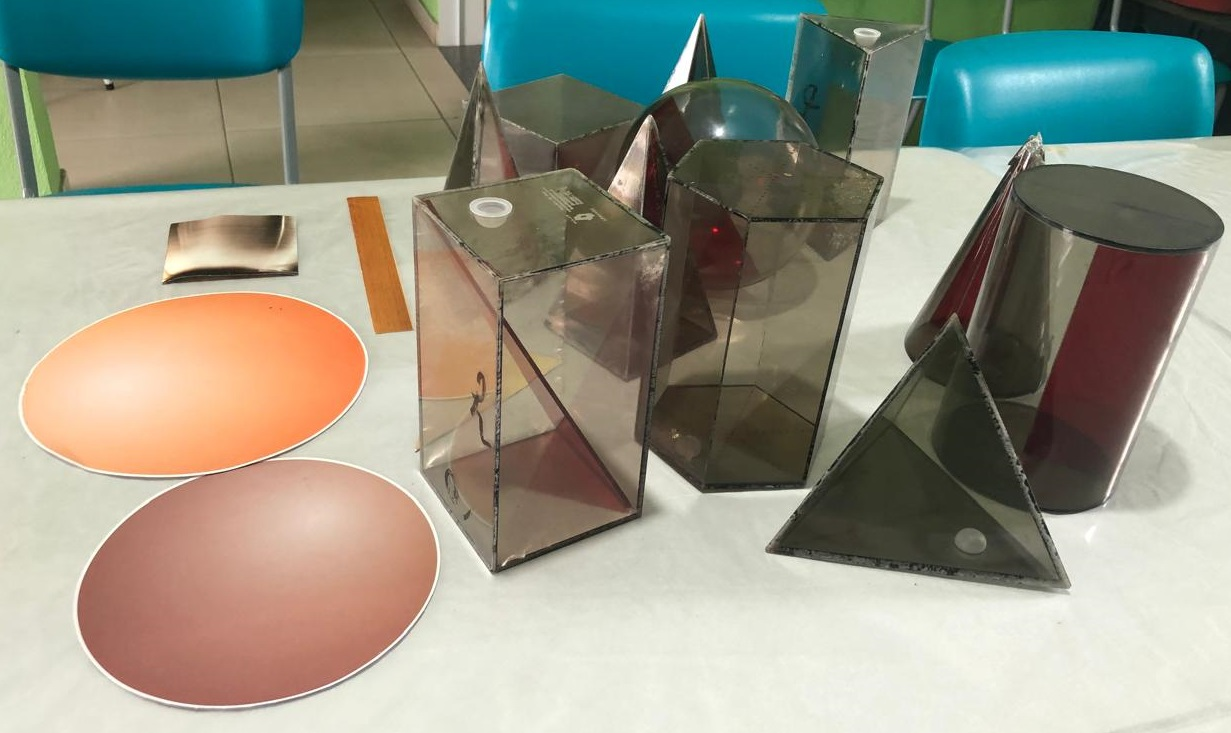
\includegraphics[width=0.5\linewidth]{Imagens/Novas imagens/Figuras Planas}
    \legend{\autoria}
\end{CenteredFigure}

Foi apresentado aos estudantes a temática a ser desenvolvida. E, nesta primeira etapa introduziu-se a geometria espacial, mostrando a diferença entre figuras bidimensionais e tridimensionais. Para isso usou-se moldes de papel no formato de triângulo, retângulo e quadrado e os sólidos geométricos, de acrílico, existentes na escola (\autoref{fig:00-Figuras planas e espaciais}). Os alunos foram instigados a observarem, detalhadamente, os sólidos geométricos e os separarem em dois grupos por semelhança. Inicialmente, separaram os que ``rolam'' (não-poliedros) daqueles que ``não rolam'' (poliedros). Foi solicitado, em seguida, que observassem apenas os poliedros e os separassem em dois subgrupos. Separaram os prismas (que possuem duas bases) das pirâmides (que possuem apenas uma base). Após esta familiarização iniciou-se a aplicação da sequência didática da resolução do problema a ser resolvido, conforme \autoref{ApendiceB}. A turma foi dividida em cinco grupos para que fosse trabalhado ao longo de toda a sequência didática.

A capacidade de entender e aplicar esses conceitos tem relevância em áreas como arquitetura, design de materiais e ciência dos materiais, onde o preenchimento eficiente do espaço pode ter implicações práticas significativas. O estudo dessas formas e suas propriedades desenvolve o pensamento espacial, a capacidade de visualizar e manipular objetos tridimensionais, habilidades cruciais em muitas áreas da ciência e engenharia.

Portanto, o estudo da geometria espacial é fundamental para compreender as propriedades e as possibilidades do espaço tridimensional, tanto em termos teóricos quanto práticos.

O problema gerador selecionado foi uma questão do ENEM-2018. Esta questão aborda o jogo Minecraft que foi criado e desenvolvido pela empresa sueca Mojang AB em 2009, sendo um sucesso mundial desde o lançamento oficial em 2011. Em 2015, a Mojang AB foi adquirida pela Microsoft e o Minecraft passou a ser disponibilizado para Xbox, Playstation e celulares. A interface gráfica é complexa, trazendo blocos tridimensionais, permitindo ao jogador a manipulação de blocos cúbicos para construção de artefatos. O principal objetivo do jogo é a sobrevivência do avatar. Para isso, com ferramentas apropriadas, deve-se iniciar colhendo madeira para fazer fogo, arar a terra para plantar, construir cercas para os animais capturados e organizar blocos para construir uma moradia, a fim de proteger-se dos inimigos (chamados \textit{creepers}) que aparecem à noite (o jogo possui um sistema sazonal, com passagem de dias, noites, estações). A interdisciplinaridade é amplamente explorável e as estratégias para sobreviver no jogo são inúmeras e concomitantes, requerendo a atenção contínua do jogador.

\subsection{Aulas 3 e 4 - Planificação Poliedros de Platão - Relação de Euler}

Nas aulas 3 e 4 voltou-se relembrando aos estudantes que a geometria espacial é tridimensional.  A escola possui uma sala \textit{maker}. Para realização das atividades desta etapa da sequência didática, os estudantes foram levados para esta sala para trabalhar em grupos, que foram anteriormente definidos.

Os objetivos destas aulas (\autoref{ApendiceC}) são:

\begin{itemize}
    \item Desenvolver a compreensão dos alunos sobre a relação entre figuras planas e sólidos geométricos através da montagem de sólidos a partir de suas planificações.
    \item Fornecer planificações de diferentes sólidos geométricos para os alunos analisarem e discutirem em grupo.
    \item Desenvolver a capacidade de construção e representação de figuras geométricas. Construir poliedros estabelecendo relações entre faces, vértices e arestas.
\end{itemize}

\subsection{Aulas 5 e 6 - Exercício de Fixação sobre a introdução de Geometria Espacial, sólidos de Platão e Relação de Euler}

Os objetivos destas aulas (\autoref{ApendiceD}) são:

\begin{itemize}
    \item Identificar poliedros côncavos e convexos.
    \item Reconhecer os sólidos platônicos.
    \item Aplicar a relação de Euler.
    \item Visualizar a transformação de uma figura plana em uma figura tridimensional (no caso, um dado) e aplicar uma propriedade específica dos dados comuns para identificar a configuração correta.
\end{itemize}

\subsection{Aulas 7 e 8 - Área Lateral e Total dos Prismas}

As aulas 7 e 8 (\autoref{ApendiceE}) têm como objetivo calcular as áreas laterais e totais dos prismas. Para isso cada grupo recebeu uma folha com as instruções a serem seguidas e também uma embalagem no formato de um prisma como descrito abaixo:

\begin{itemize}
    \item Grupo 1: Cubo - enfeite de mesa;
    \item Grupo 2: Paralelepípedo - caixa de sabonetes Natura;
    \item Grupo 3: Prisma triangular - caixa de barrinha de cereal Monama;
    \item Grupo 4: Prisma quadrangular - caixa de algodão Apolo;
    \item Grupo 5: Prisma hexagonal - caixa de biscoito Koalas Bauducco.
\end{itemize}

O problema gerador destas aulas foi calcular as áreas laterais e totais dos prismas, usando como estratégia cobrir, com papel colorido, todas as superfícies da embalagem em formato de poliedros e prismas. E, calcular a quantidade de papel que o grupo gastou para cobrir a lateral e toda a superfície do seu poliedro. Os grupos escolheram uma cor de papel laminado para cobrir seu prisma. Para calcular as áreas laterais e totais dos prismas, é importante primeiro compreender a estrutura e os componentes de um prisma. Um prisma é um sólido geométrico com duas bases paralelas congruentes e faces laterais que são quadriláteros. Com esse passo a passo, os alunos aplicaram os conceitos e fizeram os cálculos de forma prática. Garantindo assim, uma compreensão mais sólida sobre a área lateral e total de prismas diferentes.

\subsection{Aulas 9 e 10 - Exercícios de Fixação Área Lateral e Total dos Prismas}

As aulas 9 e 10, começaram com uma revisão dos conteúdos abordados na aula anterior, o que é uma prática importante para consolidar o aprendizado e conectar os conhecimentos já adquiridos com os novos. Após a revisão, foram distribuídas as folhas de exercícios de fixação (\autoref{ApendiceF}) para que fossem feitos os exercícios de revisão.

\subsection{Aulas 11 e 12 - Volume dos Prismas}

As aulas 11 e 12 (\autoref{ApendiceG}) tem como objetivo: Calcular o volume do prisma. Cada grupo recebeu o mesmo prisma da aula do cálculo da área lateral e total.

Problema Gerador: Qual a capacidade do Prisma do seu grupo, ou seja, quanto cabe nele?

Foi usado o método de deslocamento de grãos ou método de preenchimento com grãos. Este método envolve encher o prisma com grãos (como arroz ou areia) para medir o volume ocupado, sendo esta uma abordagem prática e tangível para entender e calcular volumes de formas geométricas tridimensionais.

Cada grupo recebeu um copo medidor e  certa quantidade de grãos triturados para encher completamente o seu poliedro - prisma. Em seguida, transferiram a quantidade que coube no poliedro para o copo medidor e, assim registrando quantos mililitros couberam no prisma.

Através dessa atividade, os alunos não só compreenderam as fórmulas, mas também desenvolveram um entendimento profundo dos conceitos geométricos subjacentes e suas aplicações práticas.

\subsection{Aulas 13 e 14 - Exercícios de Fixação Volume dos Prismas}

As aulas 13 e 14 buscaram fixar o conceito de volume dos prismas. O objetivo da aula é calcular, corretamente, o volume dos prismas, através da resolução dos exercícios de fixação (\autoref{ApendiceH}).

\subsection{Aulas 15 e 16 - Área Lateral e Total das Pirâmides}

Objetivo: calcular, corretamente, a área lateral e total das pirâmides.

Problema Gerador: Calcular as áreas laterais e totais das pirâmides, usando como estratégia o uso de papel colorido para cobrir toda a superfície da pirâmide e o cálculo da quantidade gasta para cobrir a embalagem.

Cada grupo recebeu uma folha com as instruções a serem seguidas (\autoref{ApendiceI}) e também um tipo de pirâmide como descrito abaixo:

\begin{itemize}
    \item \textbf{Grupo 1}: Pirâmide quadrangular (mesma altura e base do cubo recebido na aula anterior);
    \item \textbf{Grupo 2}: Pirâmide retangular (mesma altura e base do paralelepípedo recebido na aula anterior);
    \item \textbf{Grupo 3}: Pirâmide triangular (mesma altura e base do prisma triangular recebido na aula anterior);
    \item \textbf{Grupo 4}: Pirâmide quadrangular (mesma altura e base do prisma quadrangular recebido na aula anterior);
    \item \textbf{Grupo 5}: Pirâmide hexagonal (mesma altura e base do prisma hexagonal recebido na aula anterior).
\end{itemize}

Em seguida, escolheram uma cor de papel laminado para cobrir sua pirâmide. Para calcular as áreas laterais e totais das pirâmides, é importante primeiro compreender a estrutura e os componentes de uma pirâmide. Uma pirâmide é um sólido geométrico com apenas uma base e faces laterais triangulares.

\subsection{Aulas 17 e 18 - Exercícios de Fixação Área Lateral e Total das Pirâmides}

As aulas 17 e 18, começaram com uma revisão dos conteúdos abordados na aula anterior. Após a revisão, foram distribuídas as folhas de exercícios de fixação (\autoref{ApendiceJ}) para que fossem feitos os exercícios de revisão.

\subsection{Aulas 19 e 20 - Volume das Pirâmides}

As aulas 19 e 20 têm por objetivo: calcular o volume das pirâmides.

Problema Gerador: Qual a capacidade da Pirâmide, do seu grupo, ou seja, quanto cabe nele?

Cada grupo recebeu uma folha com as instruções (\autoref{ApendiceK}), grãos triturados, um prisma e uma pirâmide que possuíam a mesma altura e a mesma base.

\begin{itemize}
    \item O grupo 1 recebeu o mesmo cubo das aulas anteriores e uma pirâmide de base quadrada (mesma altura e base do cubo recebido na aula anterior);
    \item O grupo 2 recebeu o mesmo paralelepípedo das aulas anteriores e uma pirâmide de base retangular (mesma altura e base do paralelepípedo recebido na aula anterior);
    \item O grupo 3 recebeu o mesmo prisma triangular regular das aulas anteriores e uma pirâmide de base triangular (mesma altura e base do prisma triangular recebido na aula anterior);
    \item O grupo 4 recebeu o mesmo prisma quadrangular das aulas anteriores e uma pirâmide de base quadrangular (mesma altura e base do prisma quadrangular recebido na aula anterior);
    \item O grupo 5 recebeu o mesmo prisma hexagonal das aulas anteriores e uma pirâmide de base hexagonal (mesma altura e base do prisma hexagonal recebido na aula anterior).
\end{itemize}

\subsection{Aulas 21 e 22 - Exercícios de Fixação Volume das Pirâmides}

A resolução dos exercícios de fixação (\autoref{ApendiceL}) sobre Volume de Pirâmides tem como objetivo: calcular, corretamente, o volume das pirâmides.

Iniciou-se fazendo uma revisão da definição de Volume de Pirâmides e destacando que é muito importante, inicialmente, identificar a base da pirâmide para que se possa calcular, corretamente, o seu volume. Depois de entender e revisar a fórmula do volume de pirâmides, que é um terço da área da base vezes a sua altura, os grupos de alunos receberam folhas de exercícios para fixar o conceito de volume de pirâmides.

\subsection{Aulas 23 e 24 - Avaliação Final dos Poliedros - Álbum de figurinhas}

Para a avaliação foi utilizada a estratégia da confecção de um Álbum de Figurinhas sobre Poliedros.

Cada aluno recebeu um pacotinho contendo 20 figuras em papel fotográfico adesivo e um álbum impresso em forma de livreto, composto por 6 páginas com 20 espaços e sua respectiva descrição ou definição, para que o aluno pudesse identificar qual a figura deverá ser colada (\autoref{ApendiceM}).

Nesta prática, temos uma avaliação holística dos alunos, levando em conta não apenas seus conhecimentos teóricos, mas também suas habilidades práticas, criativas e sociais. A avaliação holística dos alunos é uma abordagem que visa considerar o indivíduo de maneira integral. Isso significa avaliar não apenas o conhecimento teórico, mas também habilidades práticas, criativas e sociais.

Essa prática é importante para reconhecer e valorizar diferentes aspectos do desenvolvimento e da aprendizagem dos alunos, proporcionando uma visão mais completa de suas capacidades e potencialidades.

Objetivos:

\begin{itemize}
    \item Avaliar se os alunos entendem os conceitos fundamentais dos poliedros, como faces, arestas, vértices, e como essas partes se relacionam para formar o poliedro;
    \item Verificar se os alunos conseguem visualizar e manipular mentalmente as formas geométricas, o que é crucial para a compreensão da geometria tridimensional;
    \item Observar se os alunos conseguem aplicar o conhecimento teórico na prática, identificando e colando corretamente as planificações dos poliedros;
    \item Avaliar a criatividade dos alunos na elaboração do álbum, bem como suas habilidades artísticas e de apresentação;
    \item Verificar o desenvolvimento das habilidades motoras finas através do corte, colagem e montagem das figuras;
    \item Avaliar o nível de interesse e engajamento dos alunos com a atividade, o que pode ser um indicativo de sua motivação e atitude em relação à aprendizagem da geometria.
\end{itemize}

Esta atividade avaliativa apresentou excelentes resultados, sendo muito bem recebida pelos alunos.

Foi extremamente interessante observar que cada aluno, de forma intuitiva, utilizou diferentes estratégias para facilitar a correta identificação da figura que ocuparia determinado espaço, garantindo que não fosse reutilizada. Alguns alunos numeraram o verso das figuras, outros as separaram por páginas, desenharam a figura no espaço correspondente do álbum, organizaram-nas em pilhas ou identificaram-nas com seus respectivos nomes.

Além disso, foi gratificante constatar que, ao colar a última figura, alguns alunos perceberam que haviam colocado uma figura anterior de forma incorreta, já que a figura restante não correspondia às características do espaço disponível. Eles solicitaram permissão para descolar as figuras, o que foi permitido, e conseguiram corrigir a posição, finalizando a atividade corretamente.

\chapter{Aplicação da Metodologia e Resultados} \label{cap:4_aplicacao}

Neste capítulo, são apresentadas a análise e a discussão dos dados. Os dados foram coletados através de atividades e aula prática.

Do ponto de vista da pesquisa, a finalidade foi observar o aprendizado dos estudantes e analisar as atividades realizadas por eles, uma vez que o intuito era despertar engajamento e a motivação dos estudantes nas aulas, para assim, aguçar o interesse pela aprendizagem deles.

Avaliar consiste numa etapa importante no processo de ensino e aprendizagem do aluno, e através dessas respostas foi possível organizá-las e fazer a análise dos dados.

Durante as aulas, foram aplicadas as 10 etapas do método de Resolução de Problemas propostas por \citeonline{resolucaoDeProblemas2019}. De modo geral, as aulas se iniciavam com a distribuição do material de estudo que propunha o problema, que ainda não foi trabalhado, para ser abordado em sala, foi dado um tempo para que os alunos pudessem fazer sua leitura individual, refletir e compreender o problema proposto. Em seguida, em pequenos grupos faz-se nova leitura e discutem o problema. Agora, os alunos resolvem o problema enquanto a docente acompanha de perto seus métodos e motivava os discentes em sua jornada. Os alunos registram a solução na linguagem matemática ou linguagem corrente ou desenhos. Após serem resolvidas as questões, os alunos apresentaram suas resoluções na lousa (certas, erradas ou feitas por processos diferentes) que são posteriormente discutidas com a turma para que se chegue a um consenso sobre o resultado correto. Por fim, formaliza-se o conteúdo abordado, de maneira formal e estruturada, padronizando os conceitos. Finaliza-se propondo novos problemas para consolidar o aprendizado dos alunos.

\section{Desenvolvimento e Análise da Sequência Didática}

Todos os dados obtidos foram analisados quantitativamente para descrever os sentidos, ou compreensões do assunto, contidos nas explanações. Como em todo processo de construção do conhecimento, diagnosticar a aprendizagem não é uma tarefa fácil, principalmente quando os alunos apontam não terem conhecimento sobre o conteúdo proposto.

Desse modo, analisa-se os dados buscando descobrir as fragilidades e necessidades dos estudantes, que no caso da temática da sequência de atividades, vão desde a conceituação, as práticas e cálculos.

\subsection{Análise das Aulas 1 e 2}

Nesta aula introdutória explicou-se aos estudantes a importância das práticas através das atividades/questionários (\autoref{fig:1-separando poliedros}) para seu aprendizado e como ajudará a ajustar o ensino às suas necessidades, reforçando que não é uma avaliação formal, mas uma ferramenta de diagnóstico, que será aplicado em após cada aula.

\begin{CenteredFigure}
    \caption{Separando poliedros de não-poliedros} \label{fig:1-separando poliedros}
    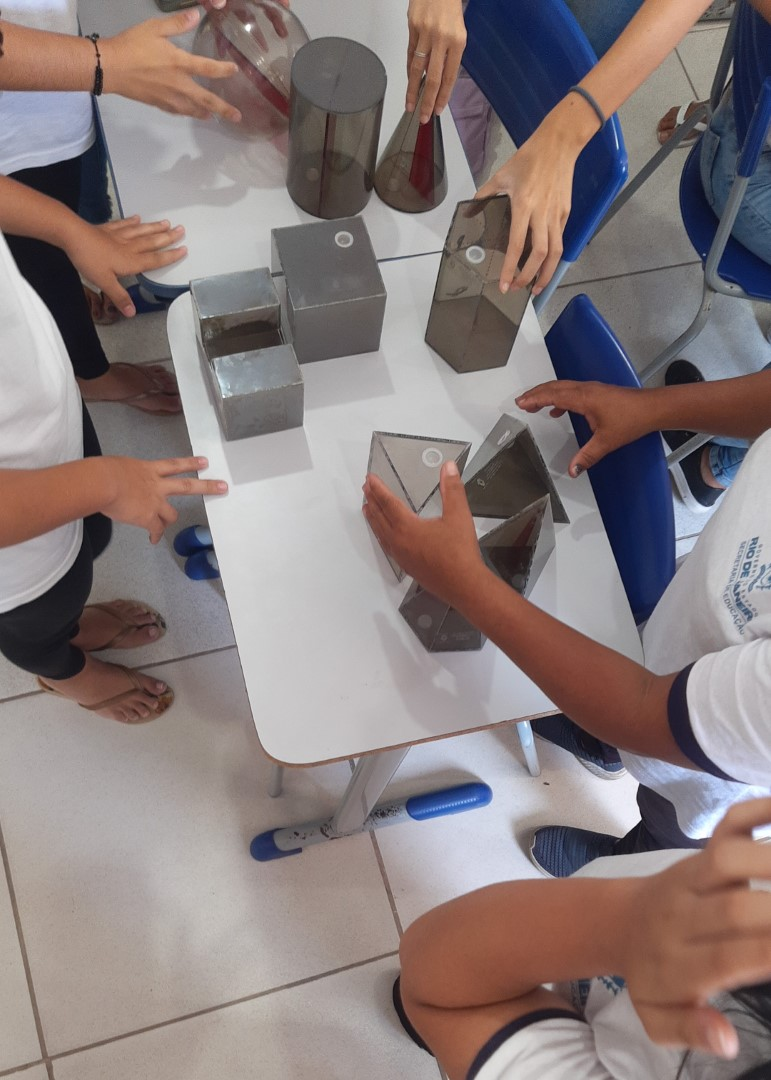
\includegraphics[width=0.5\linewidth]{01-Alunos separando os poliedros dos não-poliedros}
    \legend{\autoria}
\end{CenteredFigure}

Todos os grupos acertaram a resolução do problema gerador que foi a questão do ENEM 2018 envolvendo o jogo Minecraft (\autoref{ApendiceB}). Mas, na hora de responder o questionamento alguns grupos erraram, como observa-se na \autoref{tab:Acertos do Encontro 1}.
% e na \autoref{fig: Erros Minecraft}.

\begin{table}[htbp] \centering
    \caption{Acertos na atividade das aulas 1 e 2} \label{tab:Acertos do Encontro 1}
    \begin{tabular}{|c|c|c|c|c|c|c|}
        \hline
        \textbf{Grupos}       & \textbf{Grupo 1} & \textbf{Grupo 2} & \textbf{Grupo 3} & \textbf{Grupo 4} & \textbf{Grupo 5} \\
        \hline
        Percentual de acertos & 30               & 40               & 85               & 100              & 80               \\
        \hline
    \end{tabular}
    \legend{\legendaTabela}
\end{table}

\subsection{Análise das Aulas 3 e 4}

Problema Gerador: Verificar a relação de Euler.

Nessa aula cada grupo ficou responsável por um dos 5 poliedros platônicos (\autoref{fig:2-solidos platonicos}), da seguinte forma:  Tetraedro (grupo 1), Cubo (grupo 2), Octaedro (grupo 3), Dodecaedro  (grupo 4) e Icosaedro (grupo 5). Cada grupo recebeu sua atividade específica (\autoref{ApendiceC}), na qual determinava como deveria realizar suas 3 tarefas de construção que foram:

\begin{CenteredFigure}
    \caption{Sólidos platônicos produzidos pelos alunos} \label{fig:2-solidos platonicos}
    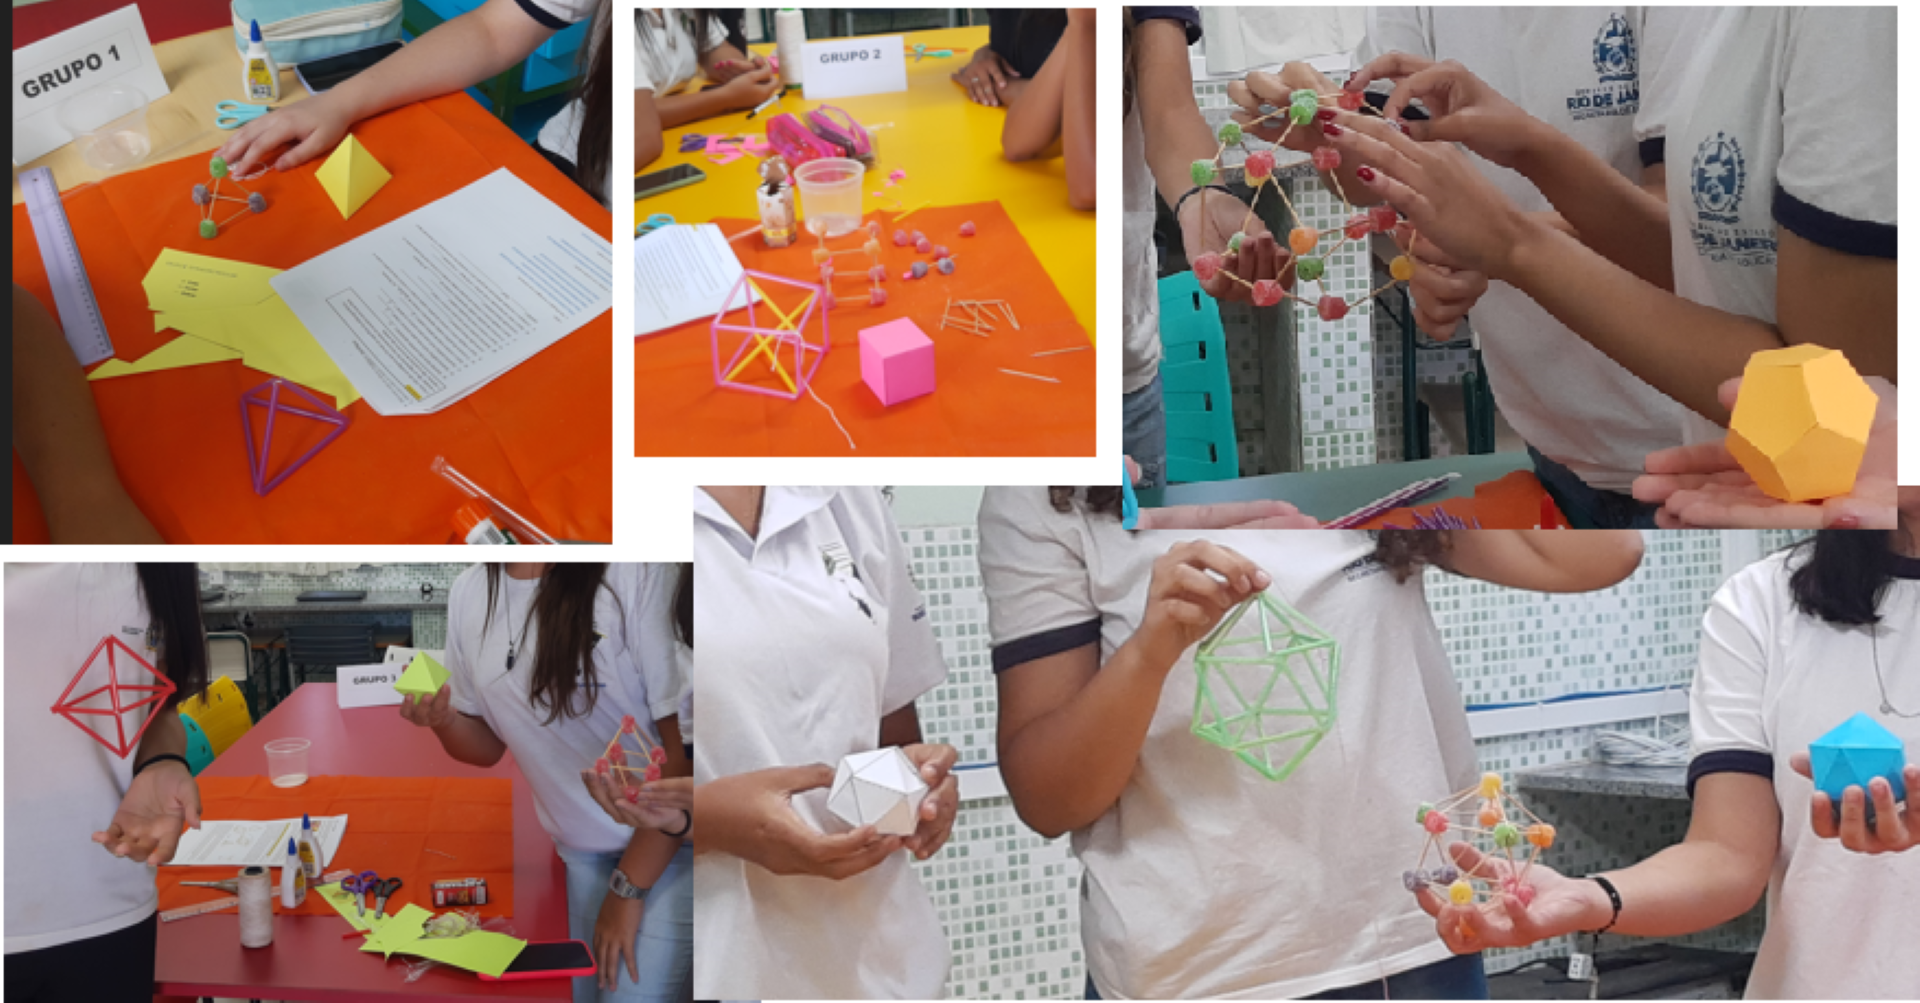
\includegraphics[width=\linewidth]{Imagens/Novas imagens/Sólidos Platônicos compilado}
    \legend{\autoria}
\end{CenteredFigure}

\begin{itemize}
    \item \textbf{1ª tarefa}:  montar o poliedro específico do seu grupo, em uma atividade de recortar, dobrar, colar e montar (modelo do tipo casca - destacando as faces);
    \item \textbf{2ª tarefa}: reproduzir o poliedro usando palitos e jujubas (modelo do tipo esqueleto - destacando os  vértices e as arestas);
    \item \textbf{3ª tarefa}: reproduzir este poliedro usando canudinhos e barbantes (modelo do tipo esqueleto - destacando as arestas).
\end{itemize}

Cada aluno pôde explorar e mostrar suas habilidades em uma das 3 tarefas. A construção dos sólidos com jujubas e canudos foi a mais interessante para eles. Mas, a tarefa com os canudos foi a mais difícil para os grupos do dodecaedro e do icosaedro, devido a quantidade de arestas. Com as três construções concluídas (\autoref{fig:2-solidos platonicos}) cada grupo registrou, na folha de atividades (\autoref{ApendiceC}), várias observações assim como o número de faces, o número de vértices e o número de arestas. E também registrou-se qual o valor encontrado para a expressão: N° vértices + N° faces - N° arestas.

O momento de maior surpresa foi ao final exposição dos trabalhos de cada grupo, onde todos perceberam que o valor encontrado para a expressão: N° vértices + N° faces - N° arestas foi o mesmo para todos os grupos, ou seja, todos encontraram o número dois.

Assim, formalizou-se a Relação de Euler para toda a classe. Esta relação foi descoberta pelo matemático suíço Leonhard Euler em 1758. Euler inicialmente desenvolveu essa fórmula para poliedros convexos, mas ela tem implicações muito mais amplas na matemática, estendendo-se a outras áreas como a topologia.

A relação de Euler, que relaciona o número de vértices (V), arestas (A) e faces (F) de um poliedro convexo é expressa da seguinte forma: \textcolor[HTML]{0000FF}{$V + F = A + 2$} ou \textcolor[HTML]{0000FF}{$V - A + F = 2$}. Esta relação para poliedros convexos é um testemunho da elegância e simplicidade da matemática, revelando uma estrutura subjacente comum a todos os poliedros convexos e estabelecendo uma base para desenvolvimentos posteriores na topologia e geometria, como mostra na \autoref{tab:Acertos do Encontro 2}.

\begin{table}[htbp] \centering
    \caption{Acertos na atividade das aulas 3 e 4} \label{tab:Acertos do Encontro 2} \begin{tabular}{|c|c|c|c|c|c|c|}
        \hline
        \textbf{Grupos}       & \textbf{Grupo 1} & \textbf{Grupo 2} & \textbf{Grupo 3} & \textbf{Grupo 4} & \textbf{Grupo 5} \\
        \hline
        Percentual de acertos & 100              & 85               & 100              & 100              & 100              \\
        \hline
    \end{tabular}
    \legend{\legendaTabela}
\end{table}

\subsection{Análise das Aulas 5 e 6}

A aula iniciou com uma revisão da aula anterior e, em seguida, cada grupo recebeu uma folha de exercícios de fixação (\autoref{ApendiceD}).

% \begin{CenteredFigure}
%     \caption{Grupo 5 resolvendo exercícios} \label{fig:3-grupo 5 exercicios}
%     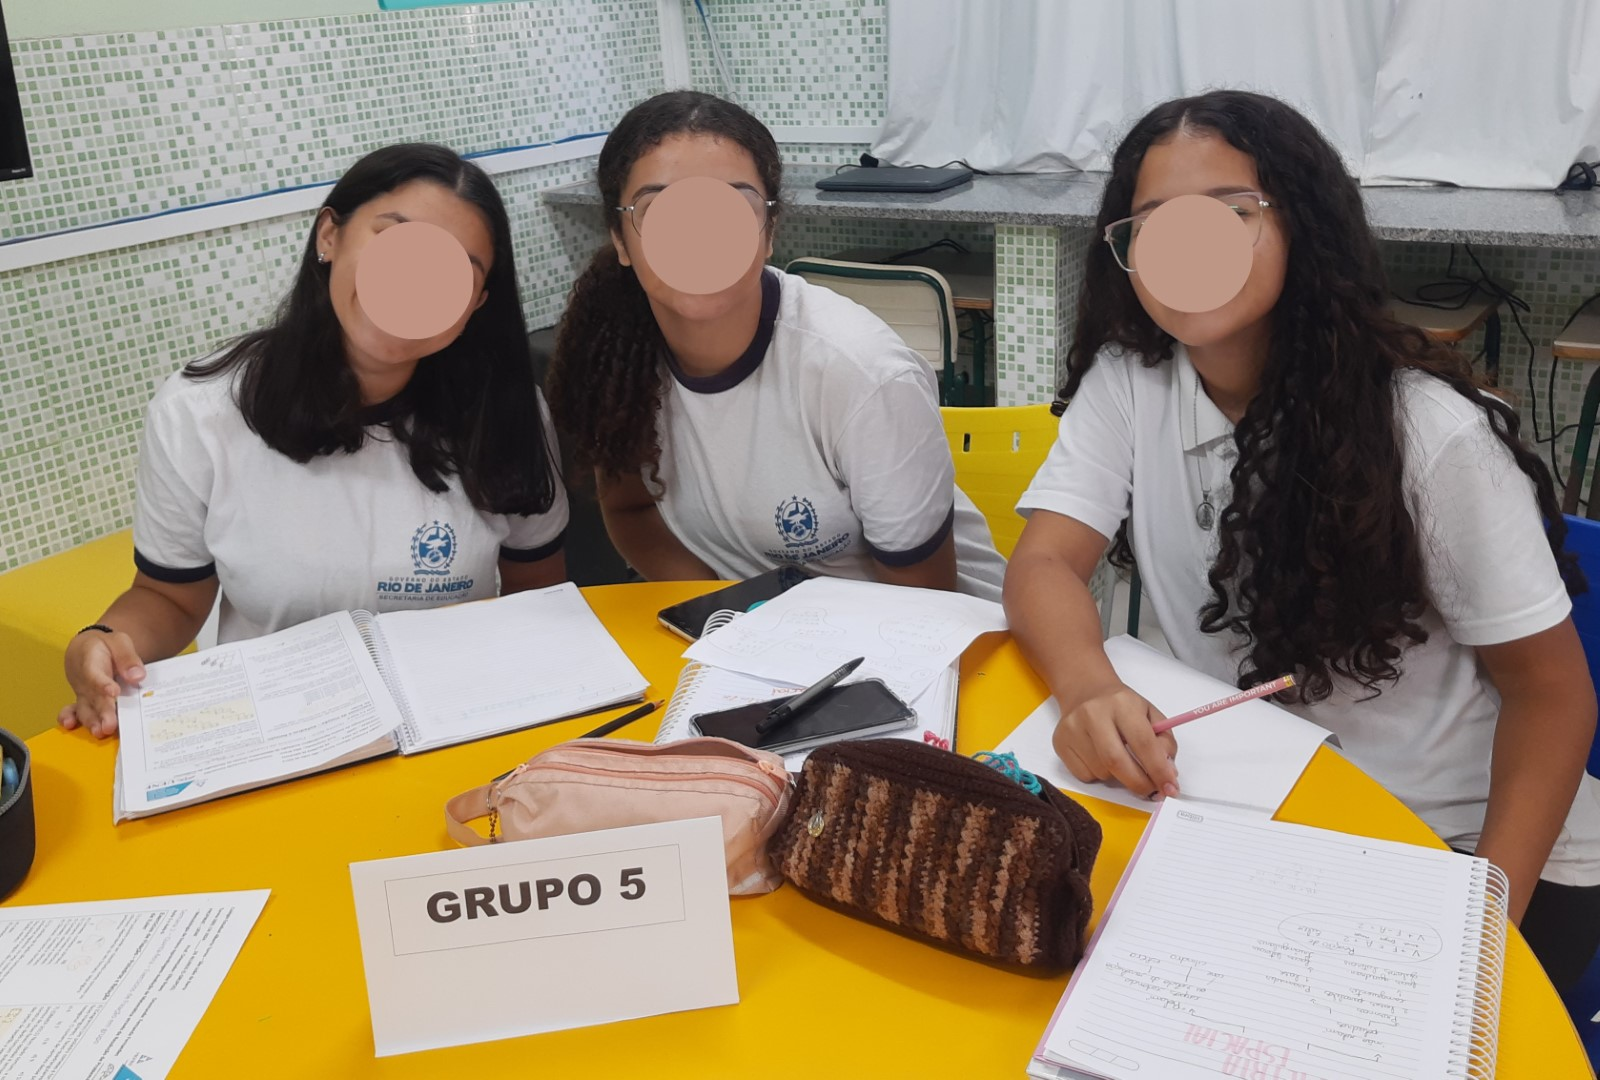
\includegraphics[width=0.5\linewidth]{03-Grupo 5 - Exercícios de fixação}
%     \legend{\autoria}
% \end{CenteredFigure}

A relação de Euler é uma ferramenta poderosa para estudar as propriedades dos poliedros convexos. Ao entender e aplicar essa relação, os alunos ganham uma compreensão mais profunda da geometria dos sólidos tridimensionais.

Analisando o aproveitamento dos grupos encontramos o seguinte resultado \autoref{tab:Acertos do Encontro 3}. E, na \autoref{fig: 250 - Aulas 5 e 6 - Questao 9 resposta certa e errada} encontra-se a resolução correta (cima) e a incorreta (baixo) da questão 9 do Exercício de Fixação das Aulas 5 e 6 (\autoref{ApendiceD}).

\begin{table}[htbp] \centering
    \caption{Acertos na atividade das aulas 5 e 6} \label{tab:Acertos do Encontro 3}
    \begin{tabular}{|c|c|c|c|c|c|c|}
        \hline
        \textbf{Grupos}       & \textbf{Grupo 1} & \textbf{Grupo 2} & \textbf{Grupo 3} & \textbf{Grupo 4} & \textbf{Grupo 5} \\
        \hline
        Percentual de acertos & 70               & 60               & 80               & 100              & 100              \\
        \hline
    \end{tabular}
    \legend{\legendaTabela}
\end{table}

\begin{CenteredFigure}
    \caption{Aulas 5 e 6 - Questão 9 resposta certa e errada} \label{fig: 250 - Aulas 5 e 6 - Questao 9 resposta certa e errada}
    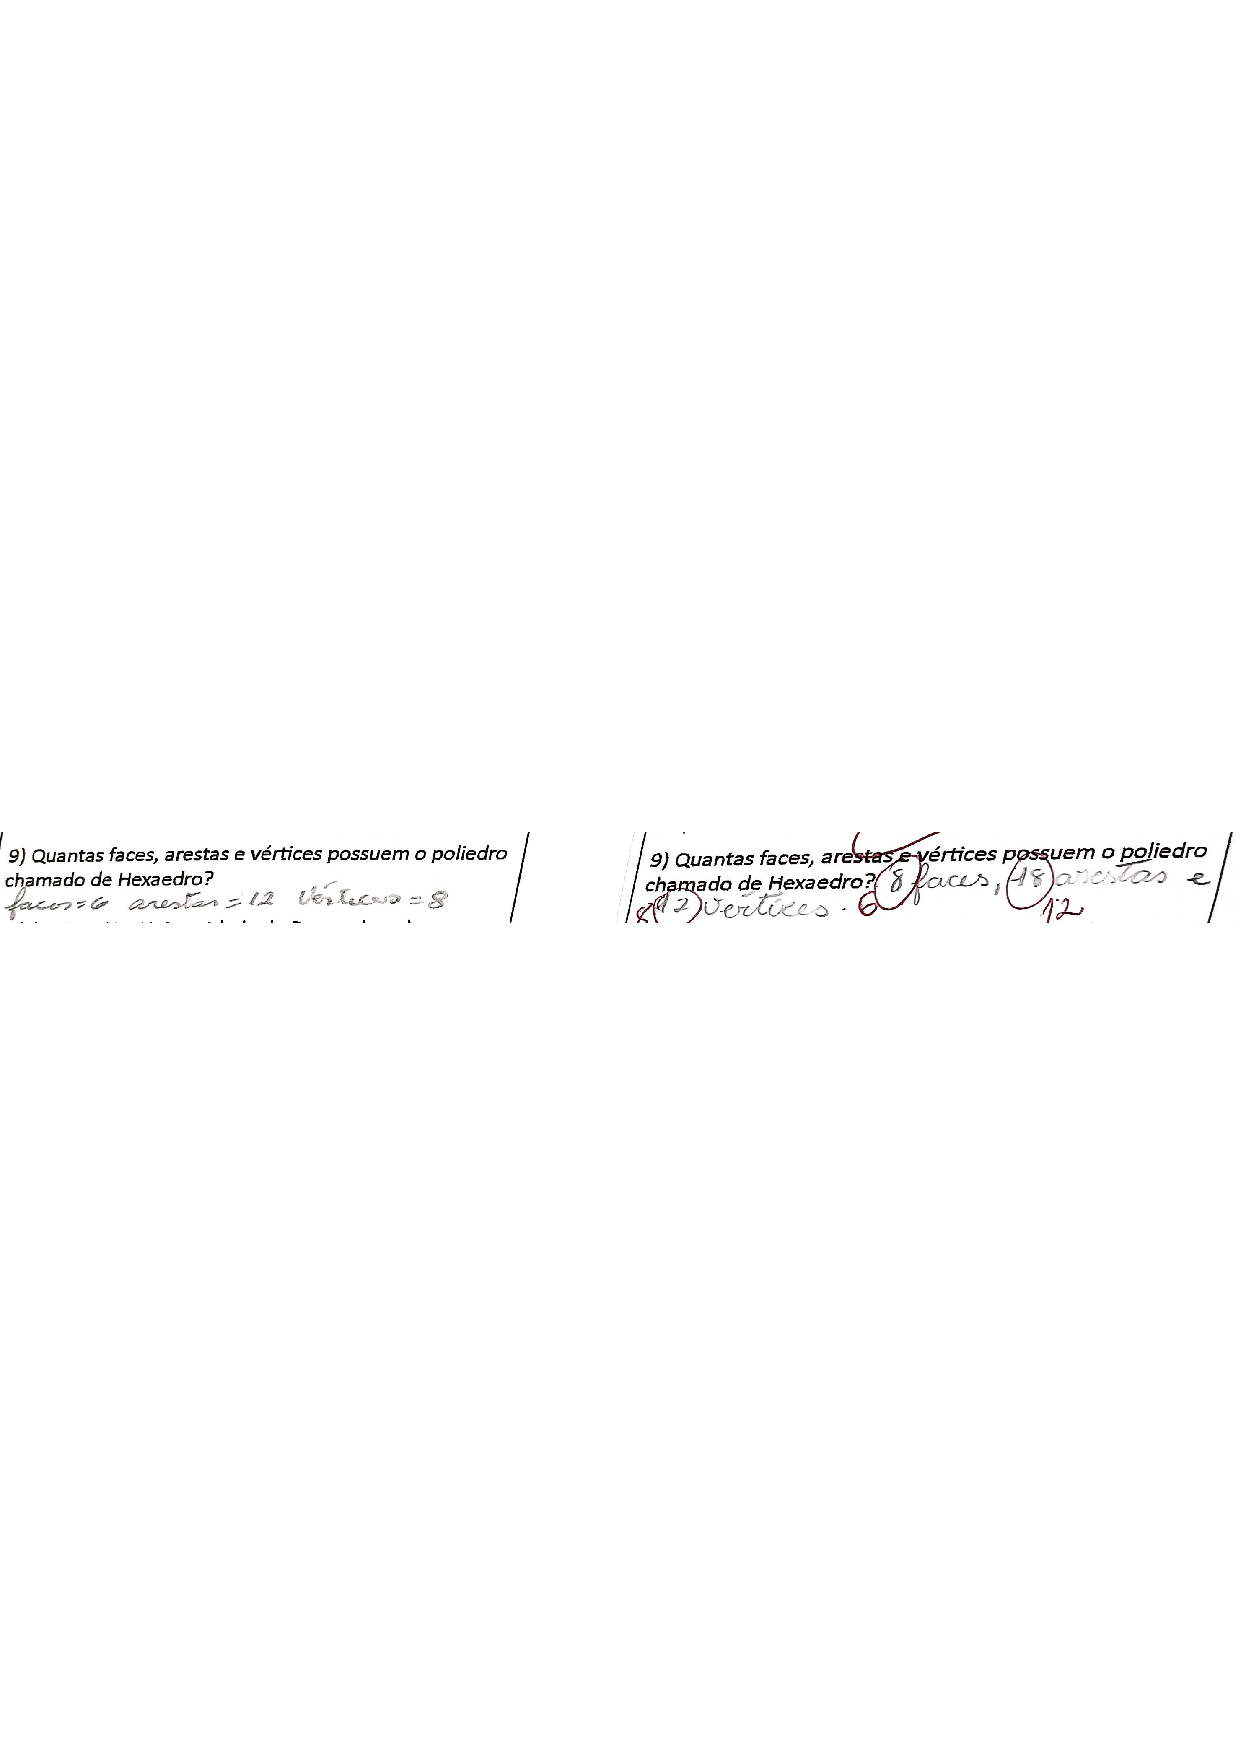
\includegraphics[width=0.8\linewidth]{Novas imagens/250 - Aulas 5 e 6 - Questão 9 resposta certa e errada}
    \legend{\autoria}
\end{CenteredFigure}

\subsection{Análise das Aulas 7 e 8}

O Problema Gerador selecionado para este encontro é: calcular a área lateral e total dos prismas. Usa-se como estratégia, cobrir, com papel colorido, todas as superfícies da embalagem em formato de poliedros - Prismas. Em seguida, calcular a quantidade de papel que o grupo gastou para cobrir a lateral e toda a superfície do poliedro.

Cada grupo recebeu um tipo de embalagem, que foram:

\begin{itemize}
    \item Grupo 1: enfeite de mesa (cubo)
    \item Grupo 2: caixa de sabonete (paralelepípedo)
    \item Grupo 3: caixa de barra de cereais (prisma triangular regular)
    \item Grupo 4: caixa de algodão (prisma quadrangular)
    \item Grupo 5: caixa de biscoito Koalas da Bauducco (prisma hexagonal regular)
\end{itemize}

Cada grupo determina a quantidade de papel necessária para cobrir a embalagem: medindo as dimensões do prisma, calculando as áreas conforme o tipo de prisma e depois somando todas essas áreas para obter a quantidade total de papel colorido necessária.

Neste problema gerador, dois grupos se destacaram na plenária, o 3 e o 5. O grupo 3, que recebeu o prisma triangular, mediu todas as dimensões, fez a planificação do prisma, fez todos os cálculos baseados na planificação e depois a colou na embalagem (\autoref{fig:4-embalagens antes}). Já o grupo 5, que recebeu o prisma hexagonal, mediu todas as dimensões, fez um grande retângulo para cobrir toda a lateral do prisma, calculou a sua área, fez as duas bases hexagonais separadas,  calculou a sua área e colou as 3 partes na embalagem (\autoref{fig:5-embalagens depois}). Os demais grupos fizeram cada face que compunha o seu respectivo prisma, calculou a sua área e colou cada face.

Este tipo de experimento foi muito apreciado por todos os alunos.

\begin{CenteredFigure}
    \caption{Embalagens antes do cálculo da área} \label{fig:4-embalagens antes}
    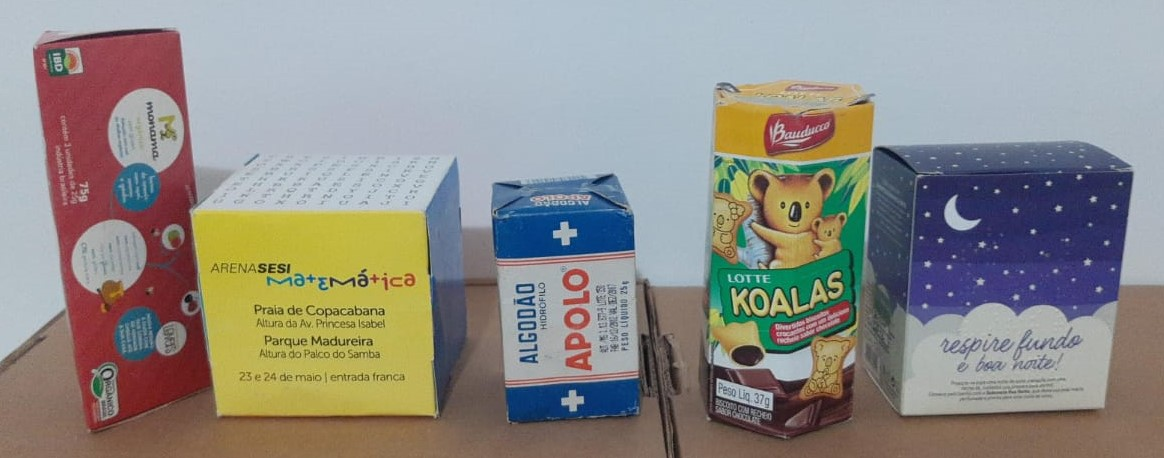
\includegraphics[width=0.5\linewidth]{04-Aulas 7 e 8 Embalagens ANTES}
    \legend{\autoria}
\end{CenteredFigure}

\begin{CenteredFigure}
    \caption{Embalagens depois do cálculo da área} \label{fig:5-embalagens depois}
    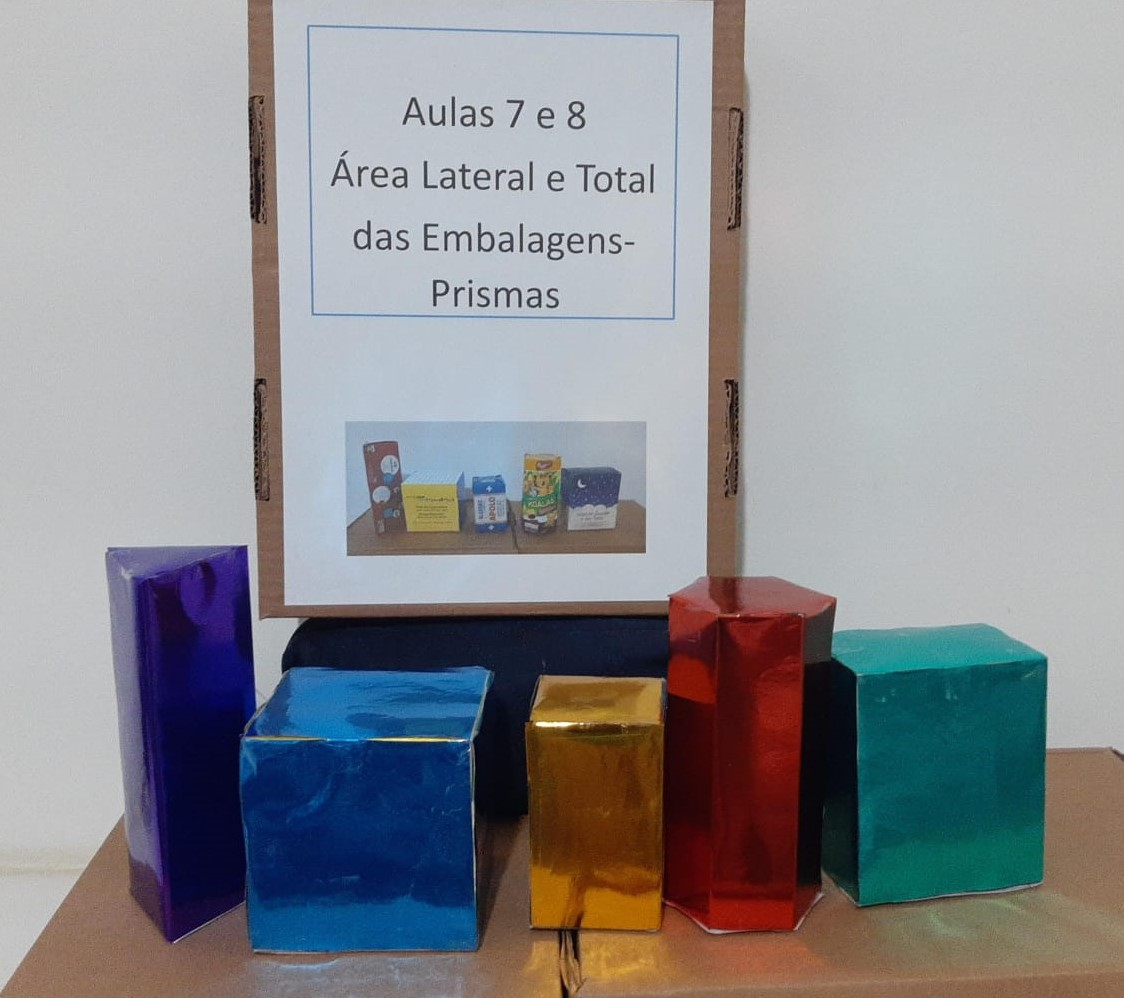
\includegraphics[width=0.5\linewidth]{05-Aulas 7 e 8 - Embalagens DEPOIS}
    \legend{\autoria}
\end{CenteredFigure}

Foi feita a formalização do conteúdo na lousa:

\textbf{Definição de Prisma}: um prisma é um poliedro composto por duas bases congruentes e paralelas, conectadas por faces laterais que são paralelogramos. O nome do prisma é dado pelo formato de sua base (por exemplo, prisma triangular, prisma hexagonal).

\textbf{Área Lateral de um Prisma}: A \textbf{área lateral} de um prisma é a soma das áreas de todas as suas faces laterais, que são paralelogramos. Para calcular a área lateral, basta multiplicar o perímetro da base pelo valor da altura do prisma.

\textbf{Fórmula da Área Lateral (AL)}: \textcolor[HTML]{0000FF}{$AL = P * h$}, onde: $P$ é o perímetro da base; $h$ é a altura do prisma (distância entre as duas bases).

\textbf{Área Total de um Prisma}: A área total de um prisma é a soma da área lateral com as áreas das duas bases.

\textbf{Fórmula da Área Total (AT)}: \textcolor[HTML]{0000FF}{$AT = AL + 2 * Ab$}, onde: $AL$ é a área lateral; $Ab$ é a área de uma das bases.

\textbf{Resumindo}: a área lateral é a superfície das faces laterais do prisma. A área total é a soma da área lateral e das áreas das duas bases.

O aproveitamento dos grupos neste encontro está registrado na \autoref{tab:Acertos do Encontro 4}.

\begin{table}[htbp] \centering
    \caption{Acertos na atividade das aulas 7 e 8} \label{tab:Acertos do Encontro 4}
    \begin{tabular}{|c|c|c|c|c|c|c|}
        \hline
        \textbf{Grupos}       & \textbf{Grupo 1} & \textbf{Grupo 2} & \textbf{Grupo 3} & \textbf{Grupo 4} & \textbf{Grupo 5} \\
        \hline
        Percentual de acertos & 100              & 0                & 80               & 20               & 40               \\
        \hline
    \end{tabular}
    \legend{\legendaTabela}
\end{table}

\begin{CenteredFigure}
    \caption{Aulas 7 e 8 - Grupo 1 acertou todos os cálculos da área lateral e total do prisma} \label{fig: 266 - Aulas 7 e 8 - Grupo 1 acertou todos os calculos da area lateral e total do prisma}
    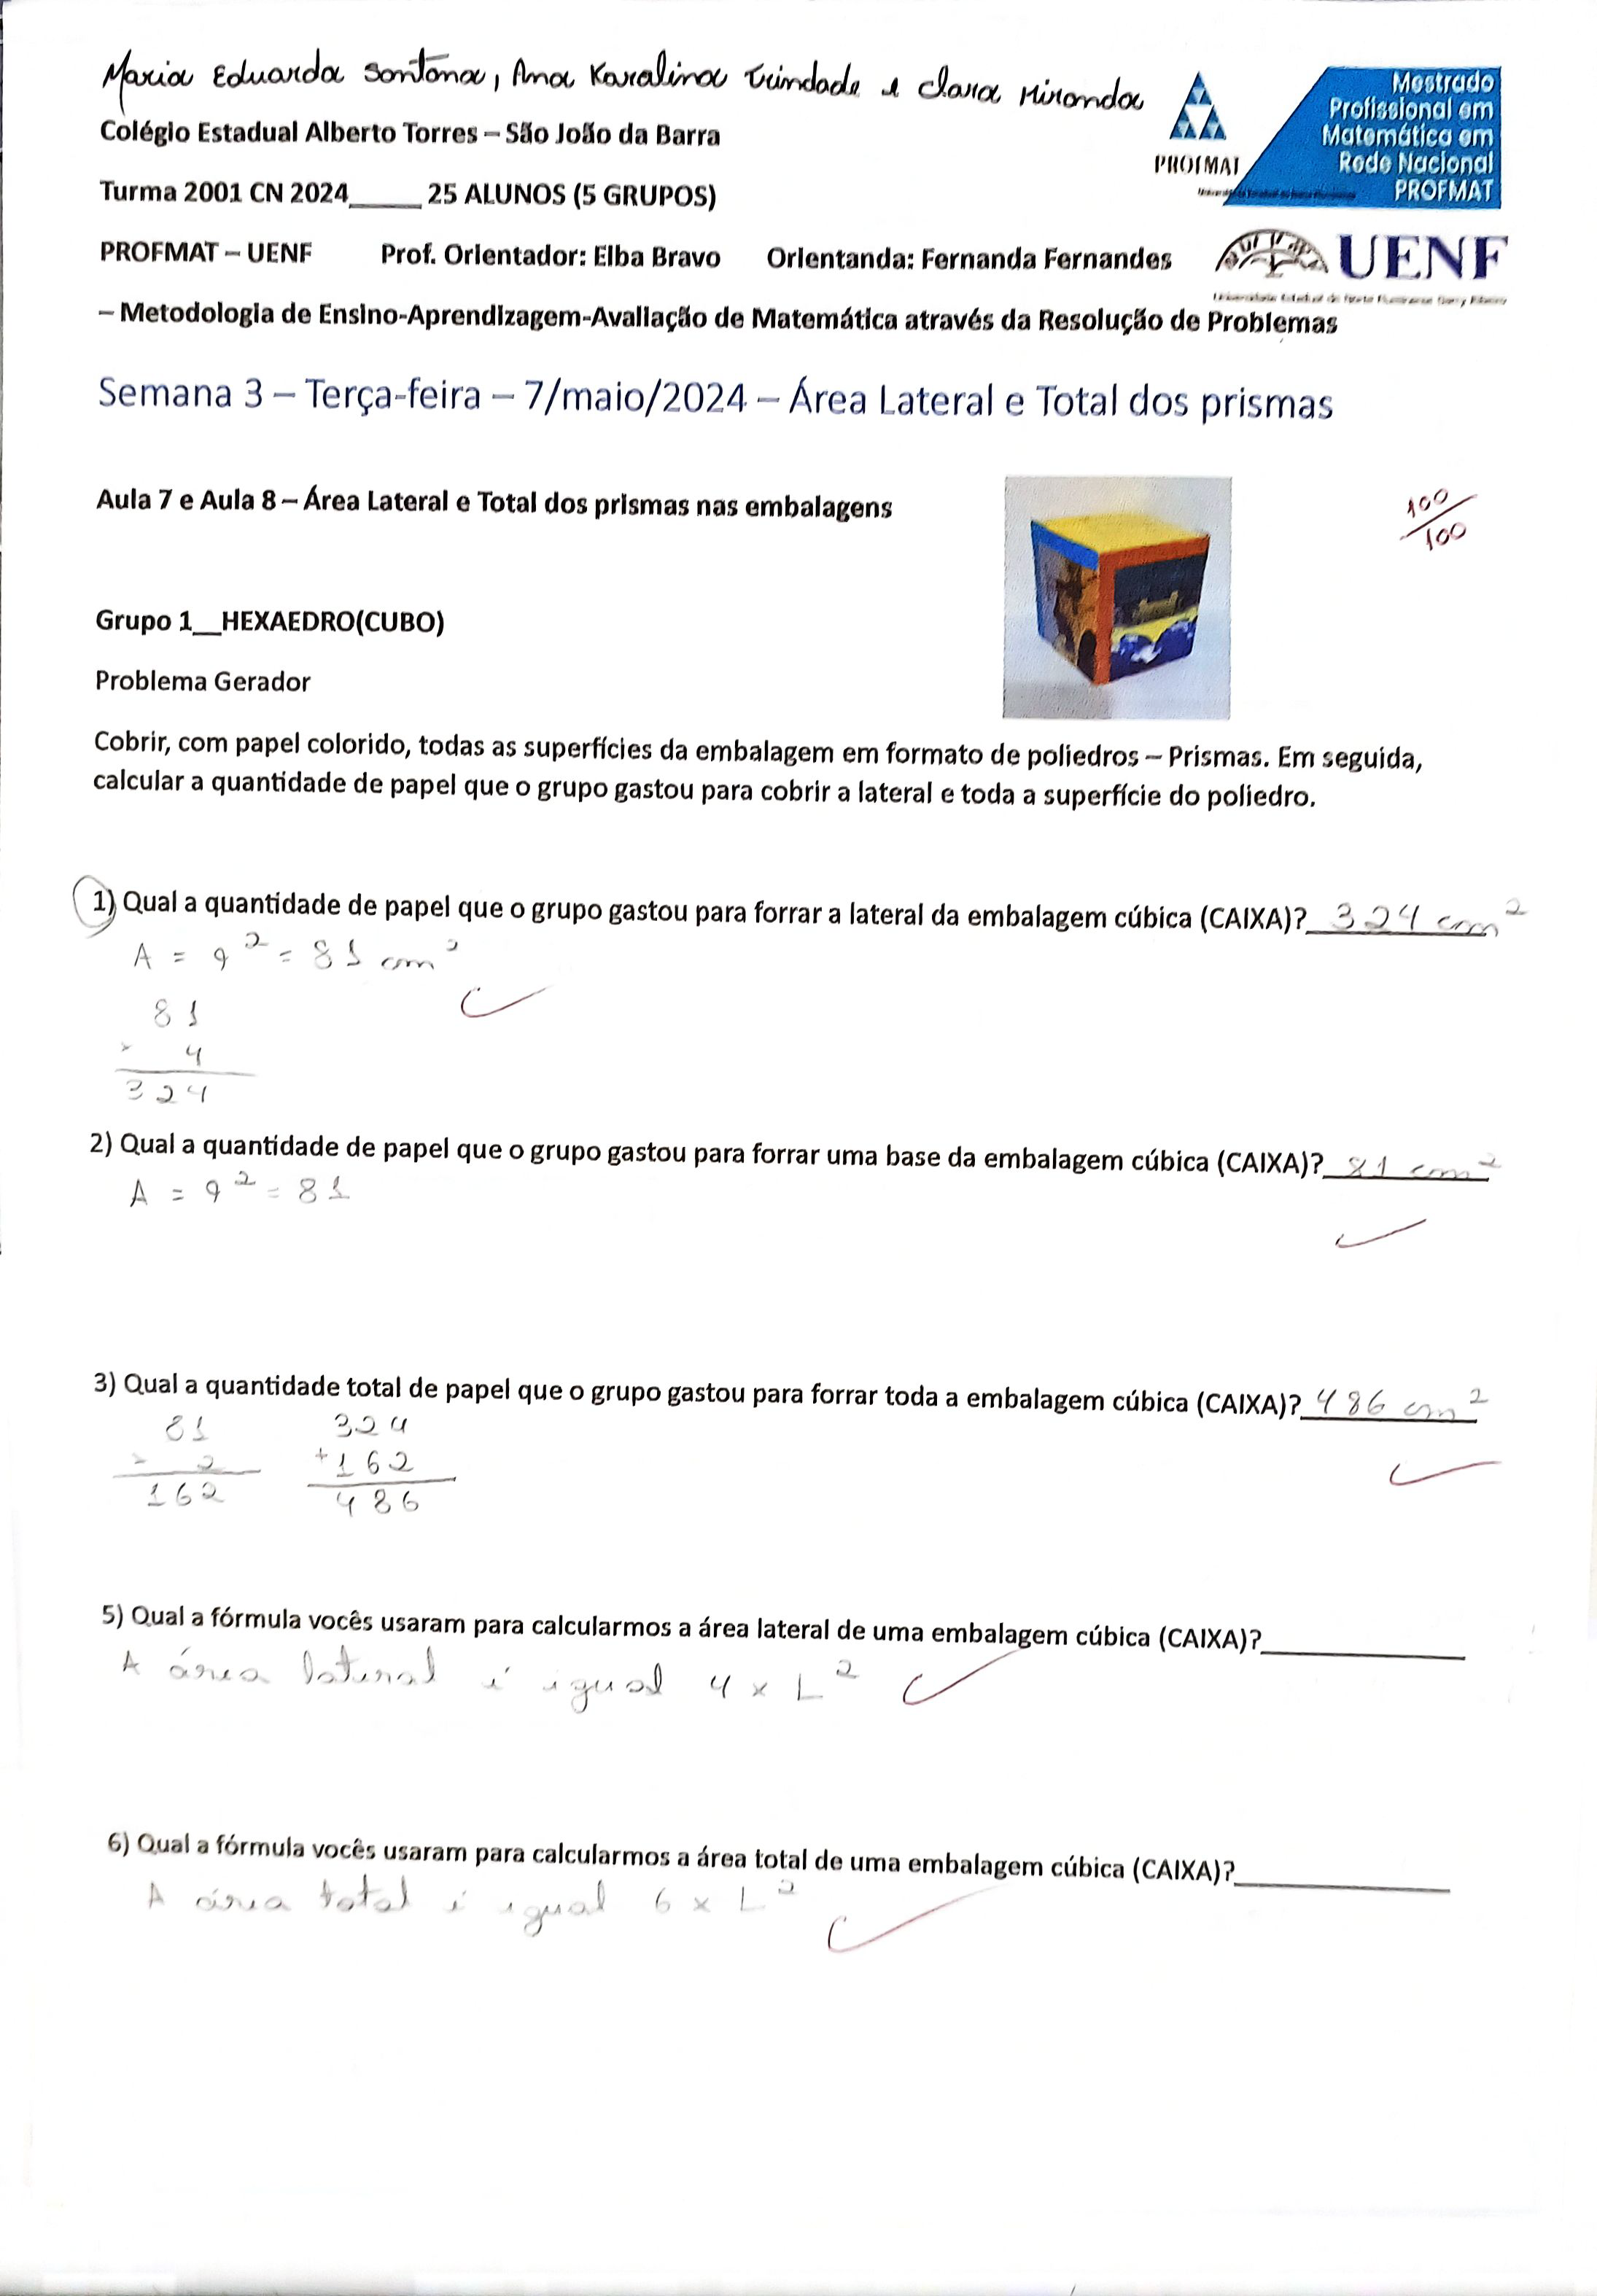
\includegraphics[width=0.7\linewidth]{Novas imagens/266 - Aulas 7 e 8 - Grupo 1 acertou todos os cálculos da área lateral e total do prisma}
    \legend{\autoria}
\end{CenteredFigure}

% \begin{CenteredFigure}
%     \caption{Aulas 7 e 8 - Grupo 2 não acertou todos os cálculos da área lateral e total do prisma} \label{fig: 267 - Aulas 7 e 8 - Grupo 2 nao acertou todos os calculos da area lateral e total do prisma}
%     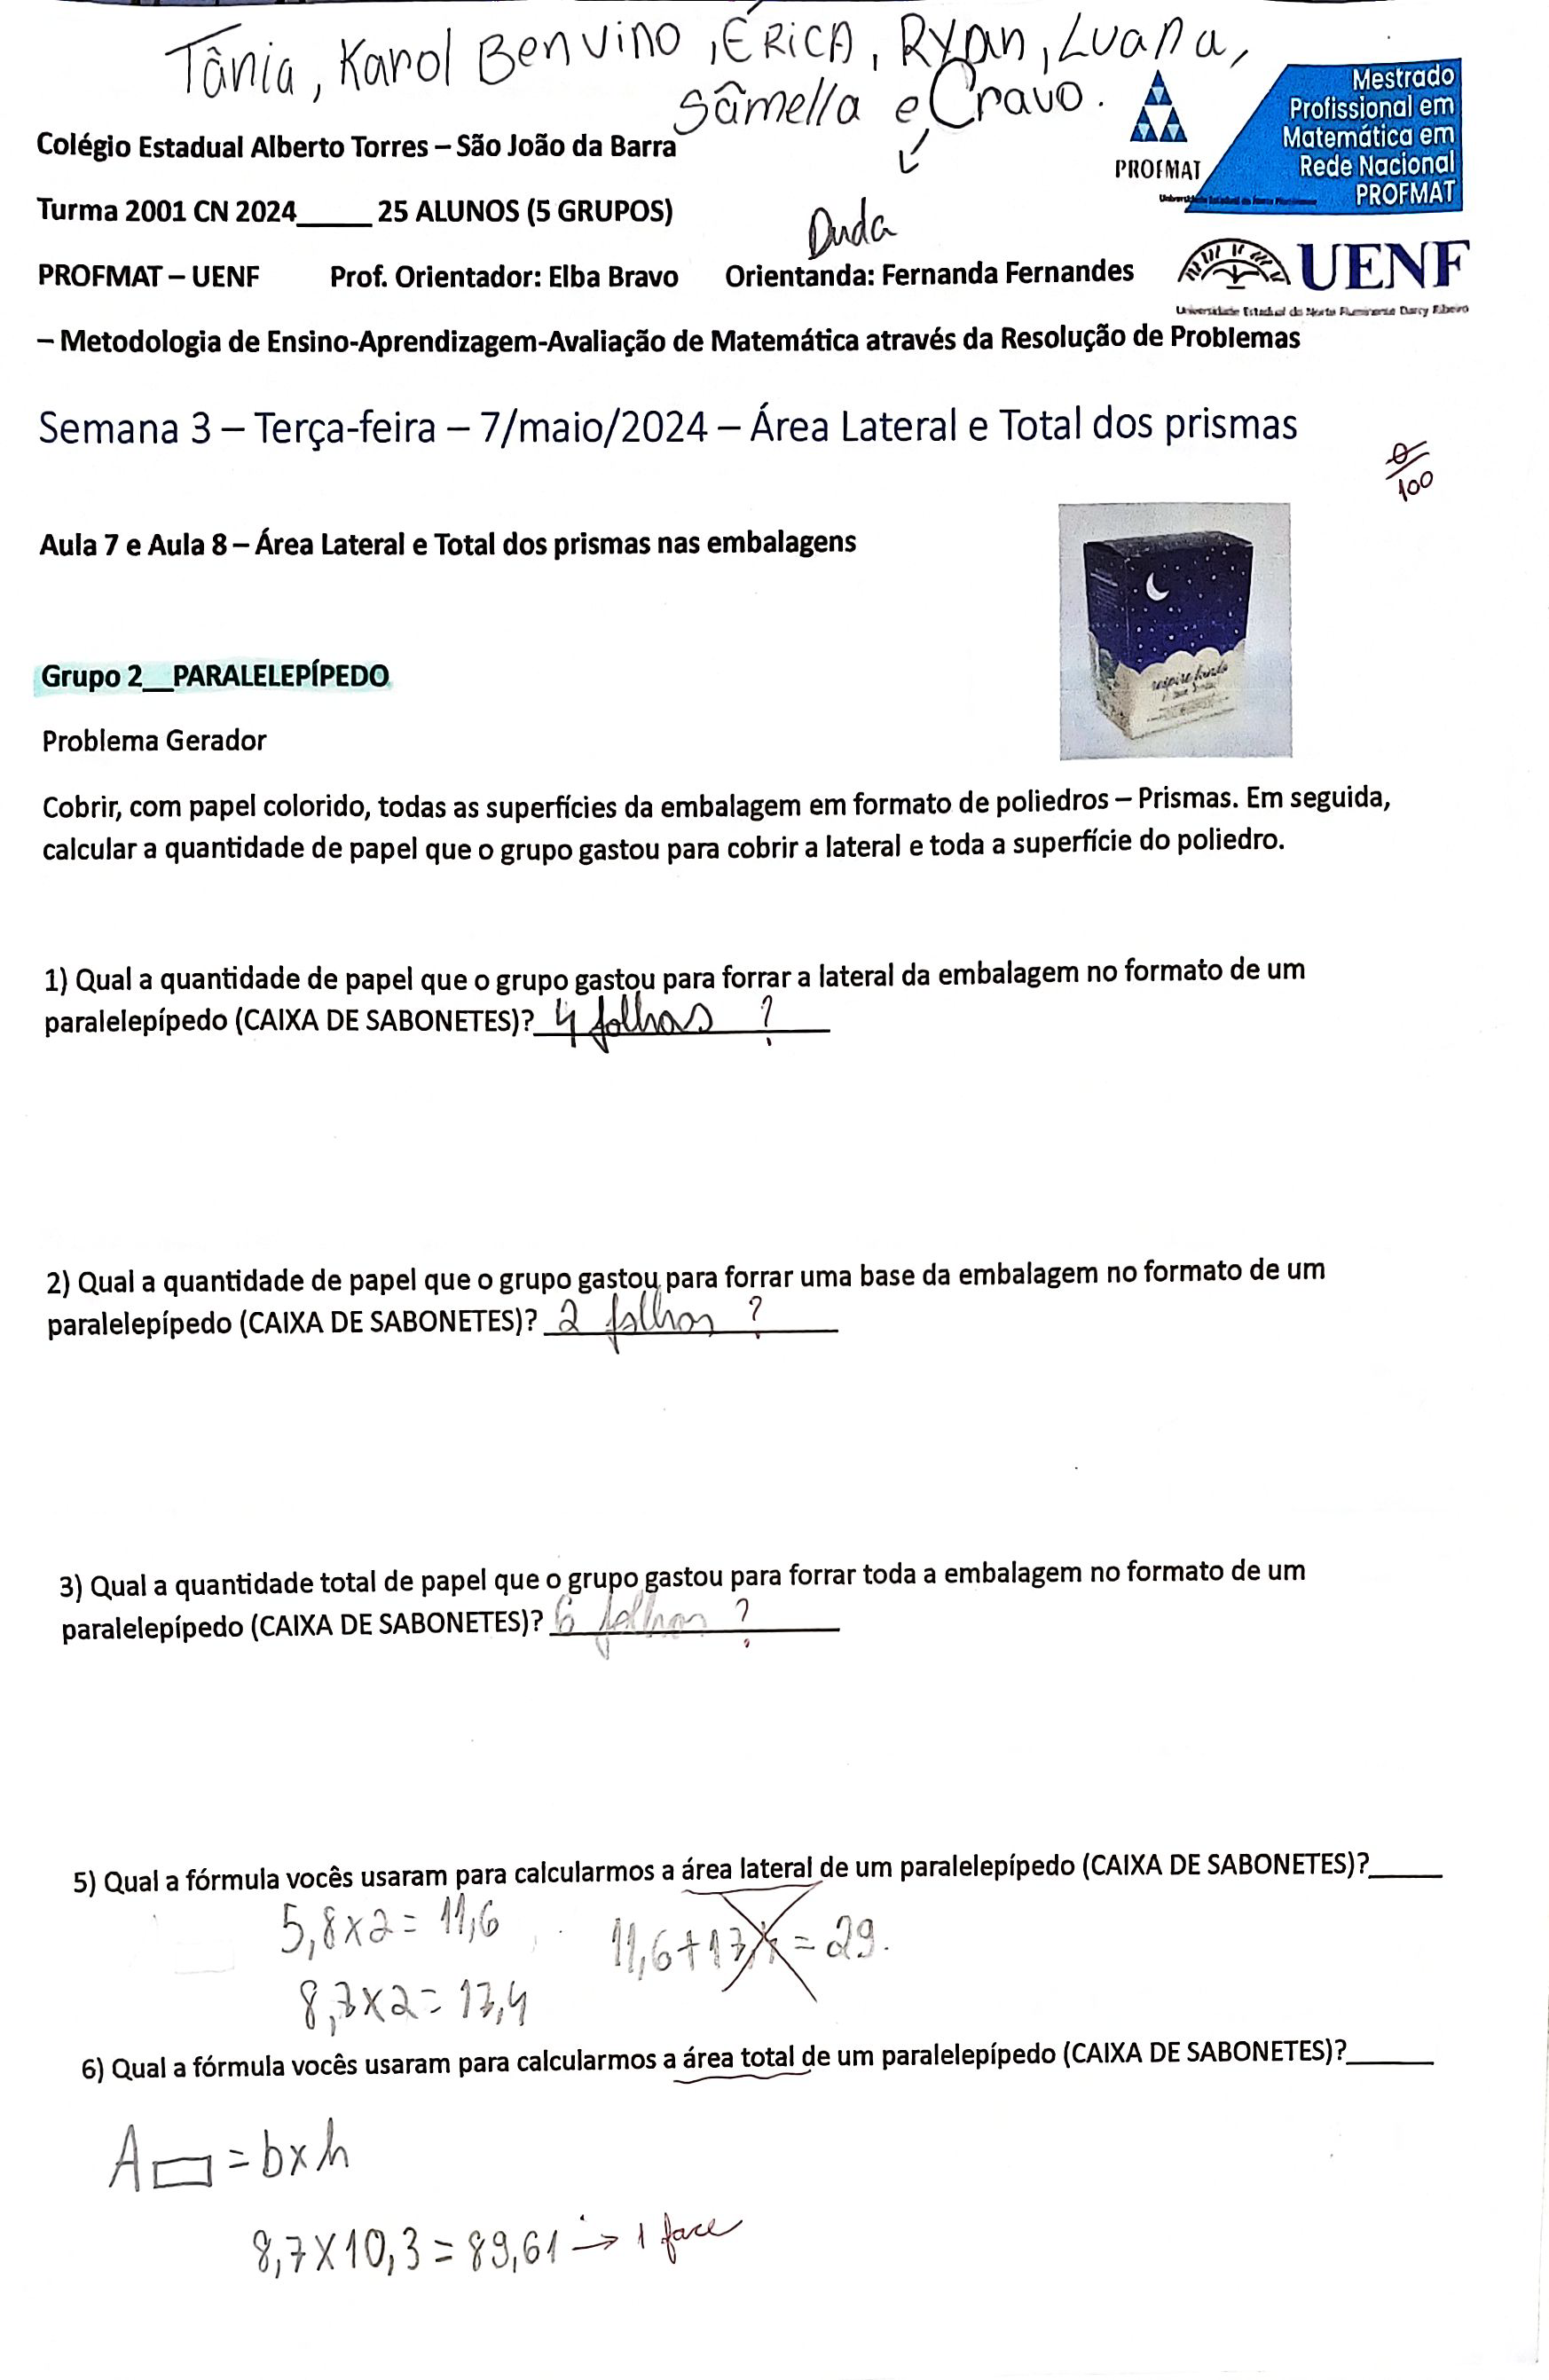
\includegraphics[width=0.5\linewidth]{Novas imagens/267 - Aulas 7 e 8 - Grupo 2 não acertou todos os cálculos da área lateral e total do prisma}
%     \legend{\autoria}
% \end{CenteredFigure}

\subsection{Análise das Aulas 9 e 10}

O objetivo deste encontro foi calcular as áreas laterais e totais dos prismas.

Foi feita uma recapitulação do conteúdo e, em seguida, cada grupo de alunos recebeu a folha de exercícios de fixação (\autoref{ApendiceF}). Esses exercícios tinham como objetivo principal reforçar a habilidade dos alunos em calcular as áreas laterais e totais de qualquer prisma, contanto que tivessem as informações necessárias sobre a forma da base, suas dimensões e a altura do prisma.

\begin{CenteredFigure}
    \caption{Grupo 3 apresentando os cálculos da questão 3} \label{fig:6-grupo 3 calculos}
    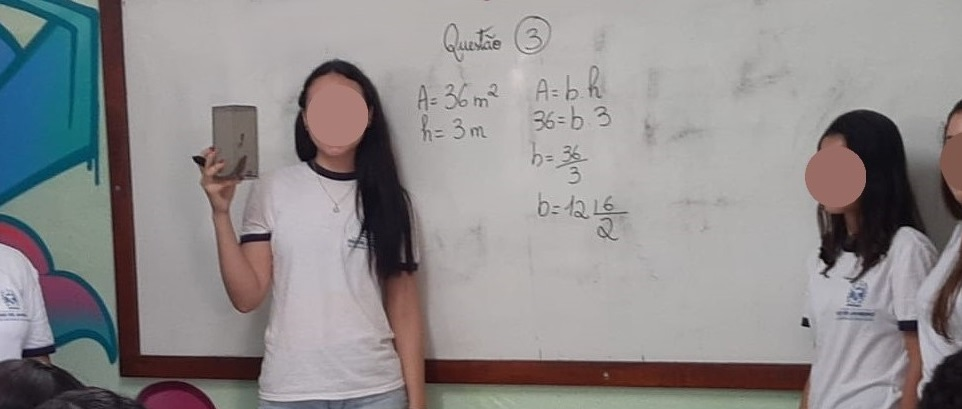
\includegraphics[width=\linewidth]{06-Grupo 3 - Apresentando seus cálculos}
    \legend{\autoria}
\end{CenteredFigure}

Em nosso dia-a-dia, é possível identificar vários elementos que possuem formato de prisma, como caixas de sapato, prédios, cômodos da casa, entre outros. E com isso trazer a nossa realidade para as aulas de geometria espacial.

\begin{table}[htbp] \centering
    \caption{Acertos na atividade das aulas 9 e 10} \label{tab:Acertos do Encontro 5}
    \begin{tabular}{|c|c|c|c|c|c|c|}
        \hline
        \textbf{Grupos}       & \textbf{Grupo 1} & \textbf{Grupo 2} & \textbf{Grupo 3} & \textbf{Grupo 4} & \textbf{Grupo 5} \\
        \hline
        Percentual de acertos & 70               & 70               & 80               & 70               & 100              \\
        \hline
    \end{tabular}
    \legend{\legendaTabela}
\end{table}

O grupo 3 se destacou ao fazer o registro da sua resolução na lousa, como mostra a \autoref{fig:6-grupo 3 calculos}. O Grupo 1 resolveu corretamente a questão 7, como mostra a \autoref{fig: 251 - Aulas 9 e 10 - Questao 7 - resposta correta}, enquanto a \autoref{fig: 252 - Aulas 9 e 10 - Questao 7 - resposta incorreta}, mostra a resolução incorreta, desta mesma questão, pelo grupo 4. A \autoref{tab:Acertos do Encontro 5} mostra o percentual de acertos dos nestas aulas.

\begin{CenteredFigure}
    \caption{Aulas 9 e 10 - Questão 7 - resposta correta} \label{fig: 251 - Aulas 9 e 10 - Questao 7 - resposta correta}
    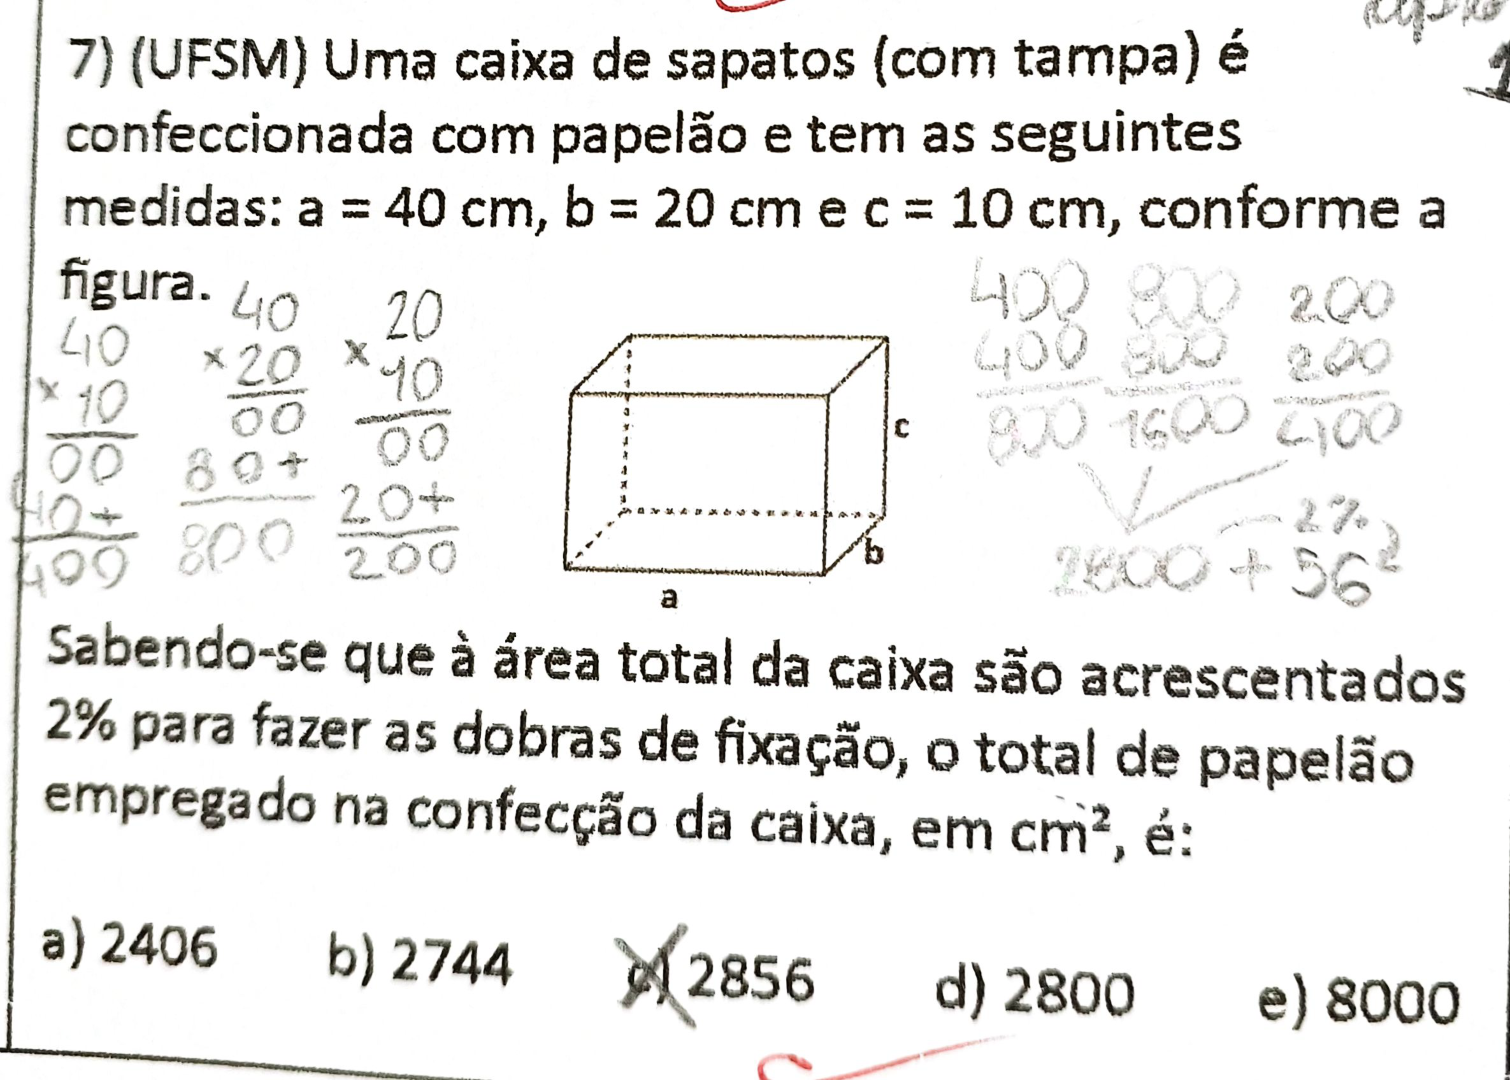
\includegraphics[width=0.5\linewidth]{Novas imagens/251 - Aulas 9 e 10 - Questão 7 - resposta correta}
    \legend{\autoria}
\end{CenteredFigure}

\begin{CenteredFigure}
    \caption{Aulas 9 e 10 - Questão 7 - resposta incorreta} \label{fig: 252 - Aulas 9 e 10 - Questao 7 - resposta incorreta}
    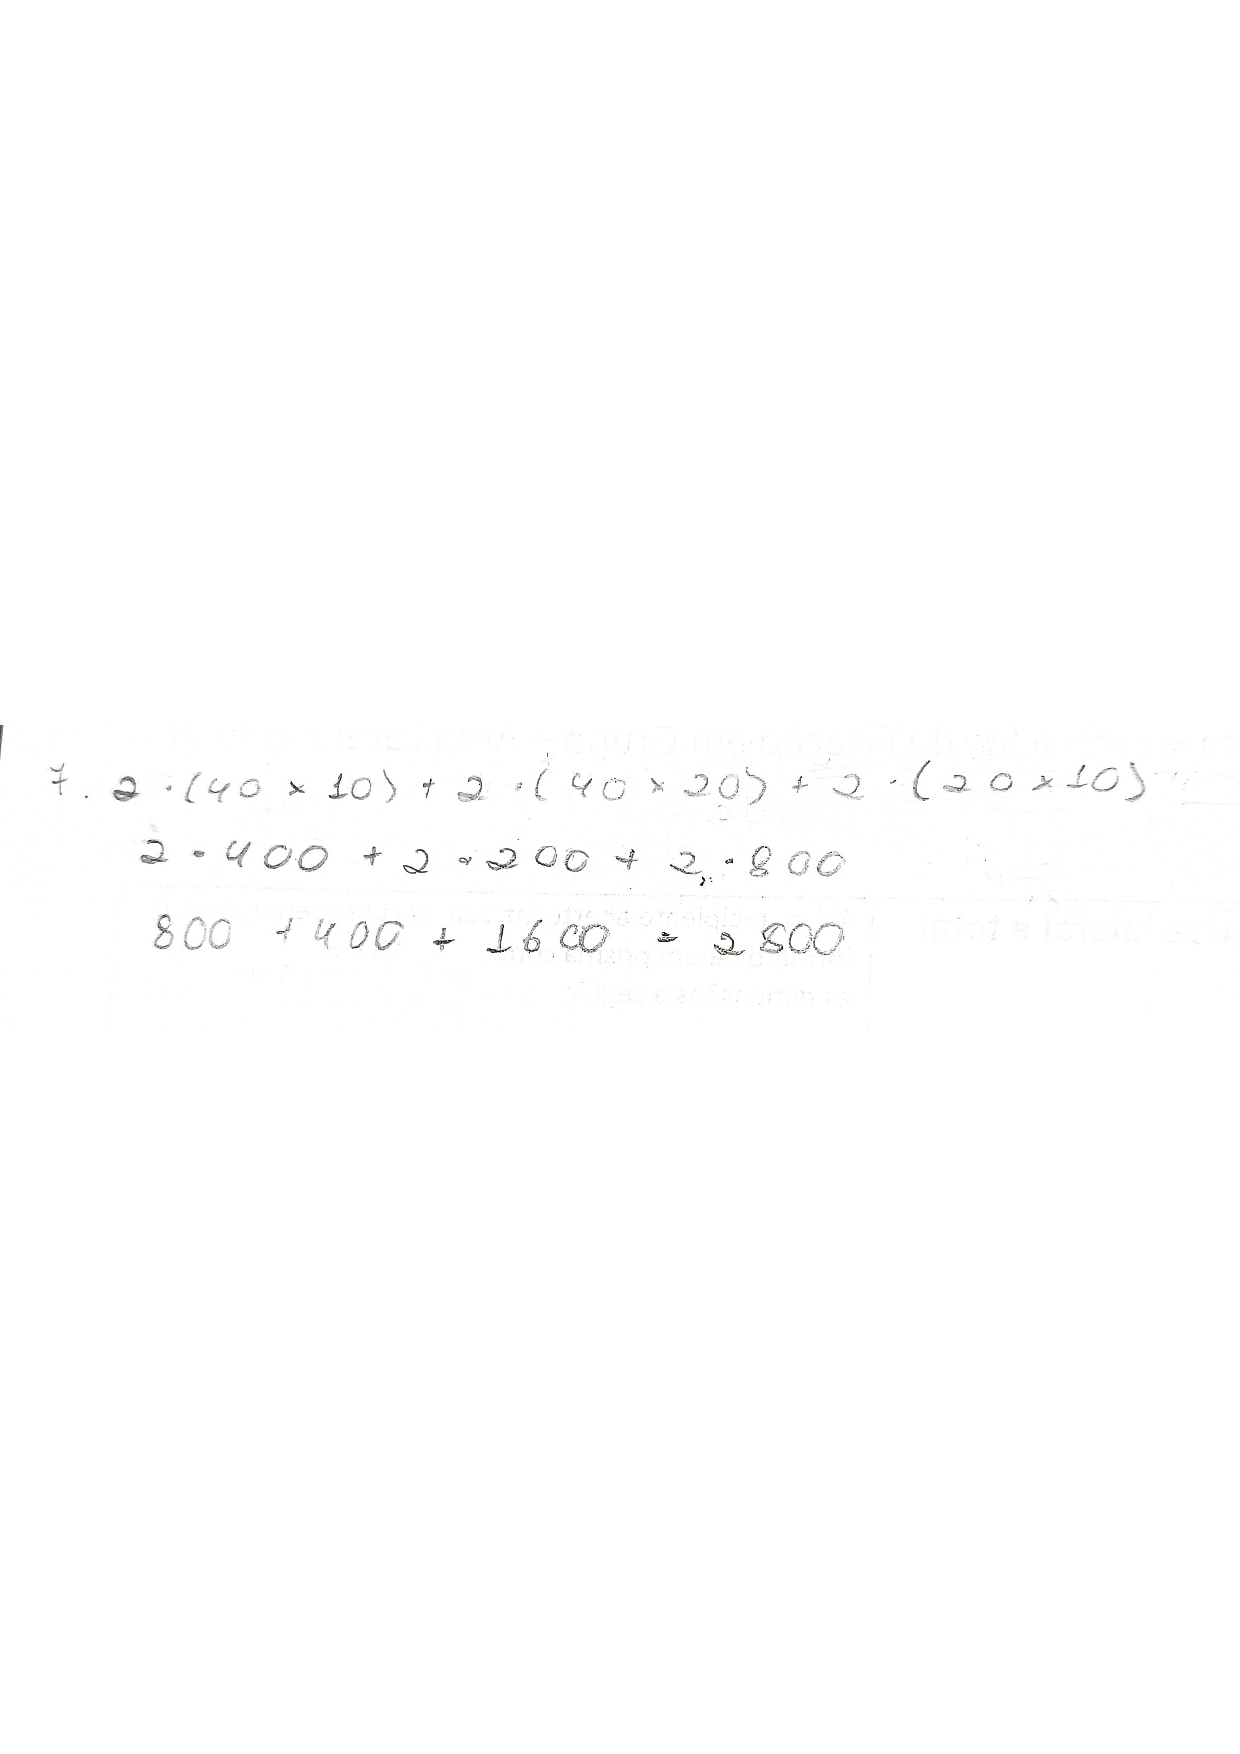
\includegraphics[width=0.5\linewidth]{Novas imagens/252 - Aulas 9 e 10 - Questão 7 - resposta incorreta}
    \legend{\autoria}
\end{CenteredFigure}

\subsection{Análise das Aulas 11 e 12}

O objetivo deste encontro foi calcular o volume dos prismas (\autoref{ApendiceH}).

Cada grupo recebeu um tipo de embalagem, que foram:

\begin{itemize}
    \item \textbf{Grupo 1}: enfeite de mesa (cubo)
    \item \textbf{Grupo 2}: caixa de sabonete (paralelepípedo)
    \item \textbf{Grupo 3}: caixa de barra de cereais (prisma triangular regular)
    \item \textbf{Grupo 4}: caixa de algodão (prisma quadrangular)
    \item \textbf{Grupo 5}: caixa de biscoito Koalas da Bauducco (prisma hexagonal regular)
\end{itemize}

Cada grupo abriu com estilete uma das bases do prisma do seu grupo e o encheu, completamente, com os grãos disponibilizados (\autoref{fig:8-medindo volume}). Transferiu-se para o medidor toda a quantidade que coube no interior do seu prisma (\autoref{fig:7-grupo 3 medindo volume prisma}) e, registraram a sua capacidade em mililitros. Fizeram as transformações de mililitro para litro, de litro para $dm^3$ e de $dm^3$ para $cm^3$. Cada grupo registrou a altura do seu prisma e também que calculou a área da base do seu respectivo prisma. Em seguida, multiplicaram a medida da altura pela área da base e compararam este resultado com o encontrado pelo medidor. Constatando assim, que os valores ficaram muito próximos.

\begin{CenteredFigure}
    \caption{Grupo 3 medindo volume do prisma triangular regular} \label{fig:7-grupo 3 medindo volume prisma}
    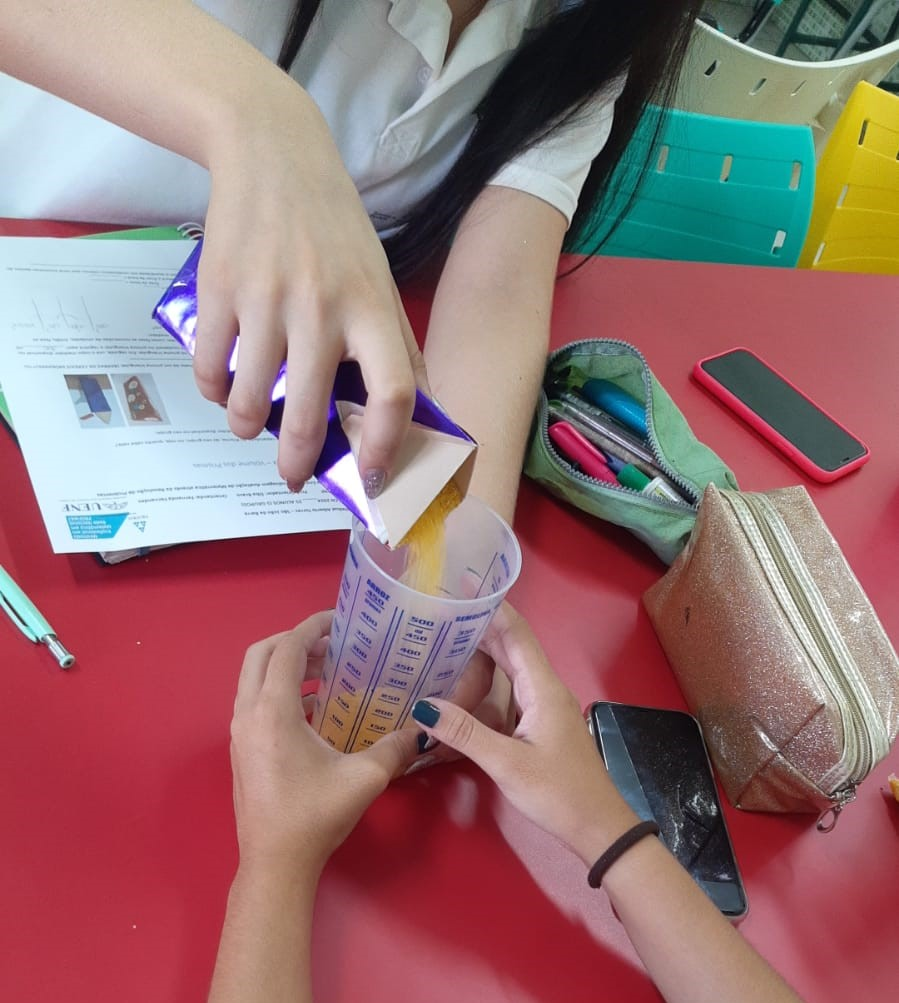
\includegraphics[width=0.5\linewidth]{07-Grupo 3 Prisma Triangular regular medindo}
    \legend{\autoria}
\end{CenteredFigure}

\begin{CenteredFigure}
    \caption{Grupo 5 medindo volume do prisma hexagonal regular} \label{fig:8-medindo volume}
    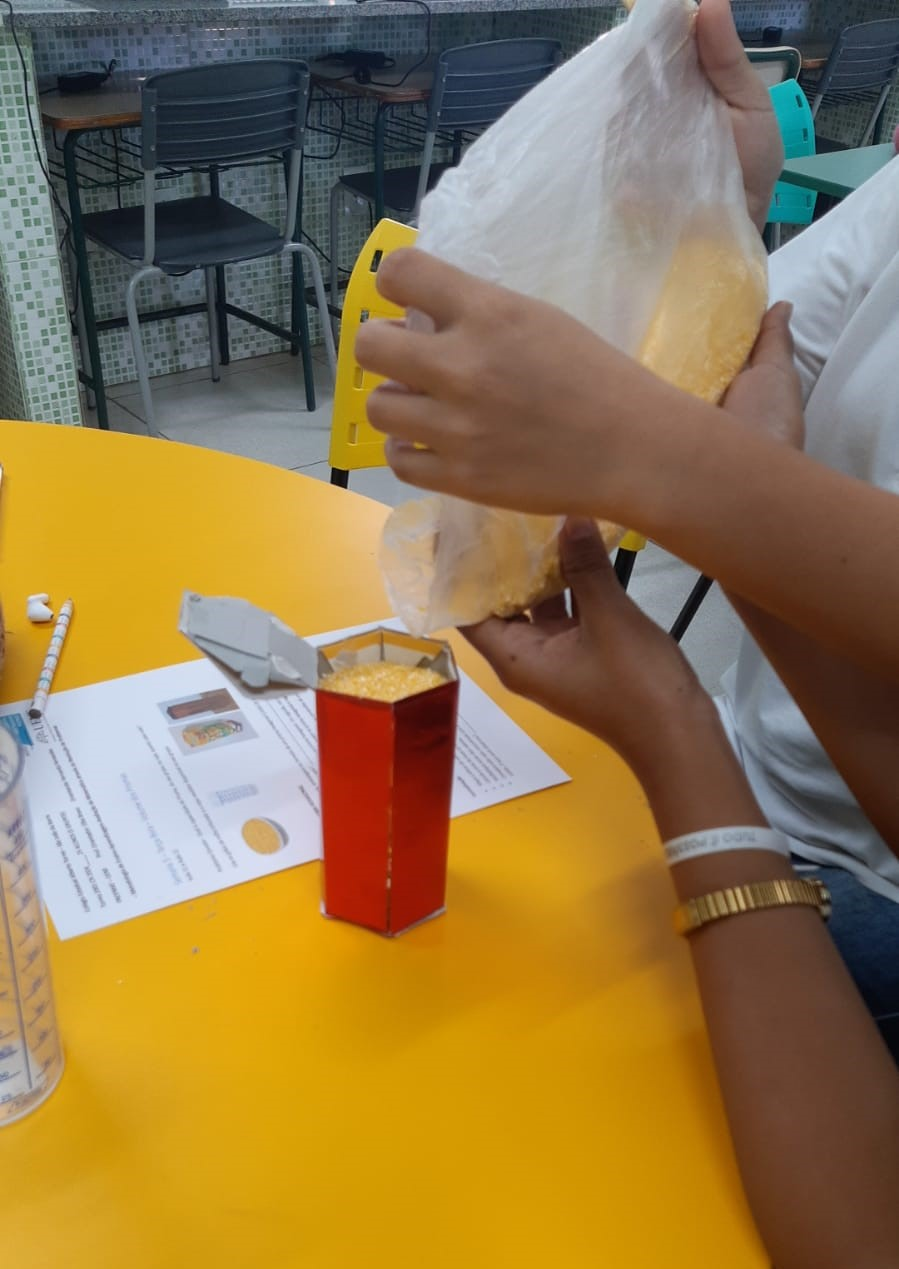
\includegraphics[width=0.5\linewidth]{08-Grupo 5 Prisma Hexagonal regular enchendo}
    \legend{\autoria}
\end{CenteredFigure}

Na plenária, percebeu-se que todos os grupos obtiveram valores muito próximos, ao comparar o volume de grãos encontrado com o valor encontrado ao multiplicar a altura do prisma pela área da base.

Formalizou-se, após a plenária, a definição de Volume de um Prisma que é: a quantidade de espaço que ele ocupa no espaço tridimensional. Para encontrar o volume de um prisma, multiplicamos a área da base pela altura (a distância entre as duas bases paralelas). Logo, conclui-se que o volume de um prisma depende da forma de sua base e da sua altura.

Passos para calcular a capacidade (volume) de um prisma:

\begin{enumerate}
    \item Identificar a forma da base: Um prisma pode ter várias formas de base, como retangular, triangular, hexagonal, etc.
    \item Calcular a área da base: Use a fórmula apropriada para a forma da base.
    \item Multiplicar a área da base pela altura do prisma. Lembrando que, a altura é a distância entre as duas bases paralelas.
\end{enumerate}

\textbf{Fórmula do Volume de um Prisma}: o volume de um prisma pode ser calculado utilizando a seguinte fórmula:

\textcolor[HTML]{0000FF}{$V = Ab * h$}

Onde: $V$ é o volume do prisma, $Ab$ é a área da base do prisma e $h$ é a altura do prisma (distância entre as duas bases).

Este tipo de experimento foi amplamente apreciado por todos os alunos.

\begin{table}[htbp] \centering
    \caption{Acertos na atividade das aulas 11 e 12} \label{tab:Acertos do Encontro 6}
    \begin{tabular}{|c|c|c|c|c|c|c|}
        \hline
        \textbf{Grupos}       & \textbf{Grupo 1} & \textbf{Grupo 2} & \textbf{Grupo 3} & \textbf{Grupo 4} & \textbf{Grupo 5} \\
        \hline
        Percentual de acertos & 100              & 100              & 100              & 100              & 100              \\
        \hline
    \end{tabular}
    \legend{\legendaTabela}
\end{table}

\subsection{Análise das Aulas 13 e 14}

Neste encontro o objetivo foi fixar e calcular, corretamente, o volume dos prismas. Iniciou-se fazendo uma recapitulação da definição de volume e destacando que é muito importante, inicialmente, identificar a base do prisma para que se possa calcular, corretamente, a sua área. E que em seguida, para se calcular corretamente o volume do prisma basta multiplicar a área da base pela altura do prisma (\autoref{ApendiceH}). Em seguida, cada grupo recebeu a sua folha de exercícios de fixação do conceito de volume de prisma. Cada grupo apresentou sua solução a serem analisadas e debatidas na plenária.

% \begin{CenteredFigure}
%     \caption{Resolvendo exercícios} \label{fig:9-grupo 5 exercicios fixacao}
%     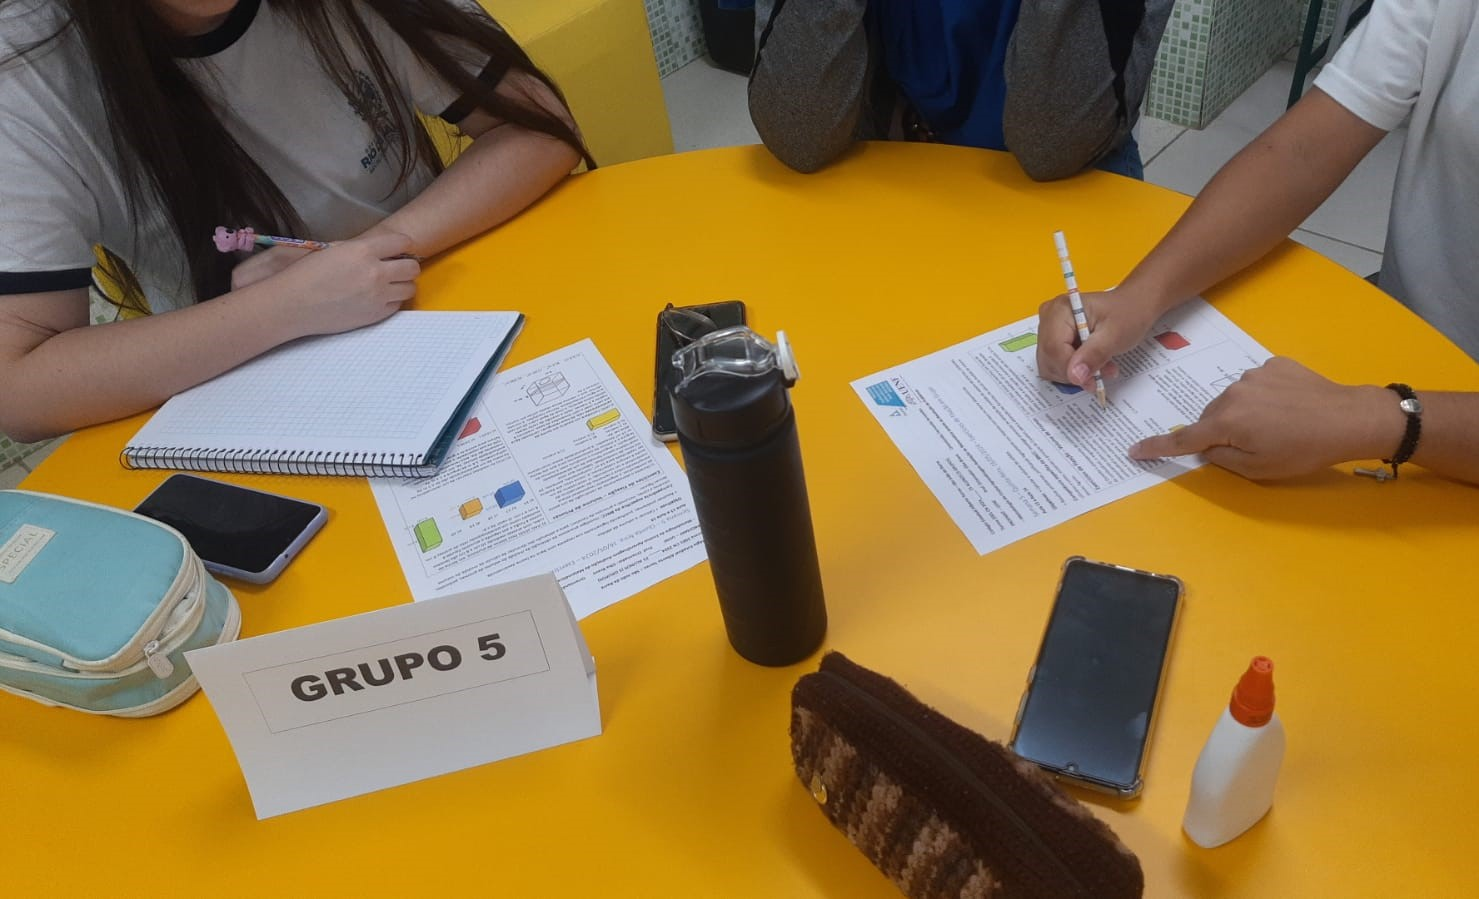
\includegraphics[width=0.5\linewidth]{09-Grupo 5 Exercícios Fixação Volume Prismas}
%     \legend{\autoria}
% \end{CenteredFigure}

O grupo 2 não teve 100\% de acerto, como mostra a \autoref{tab:Acertos do Encontro 7}. Este grupo apresentou certa dificuldade para entender e resolver algumas questões, como mostrada na \autoref{fig: 254 - Aulas 13 e 14 - Questao 5 - resposta incorreta}. Enquanto os demais grupos responderam corretamente a mesma questão, como mostra a \autoref{fig: 253 - Aulas 13 e 14 - Questao 5 - resposta correta}.

\begin{table}[htbp] \centering
    \caption{Acertos na atividade das aulas 13 e 14} \label{tab:Acertos do Encontro 7}
    \begin{tabular}{|c|c|c|c|c|c|c|}
        \hline
        \textbf{Grupos}       & \textbf{Grupo 1} & \textbf{Grupo 2} & \textbf{Grupo 3} & \textbf{Grupo 4} & \textbf{Grupo 5} \\
        \hline
        Percentual de acertos & Faltou           & 70               & 100              & 100              & 100              \\
        \hline
    \end{tabular}
    \legend{\legendaTabela}
\end{table}

\begin{CenteredFigure}
    \caption{Aulas 13 e 14 - Questão 5 - resposta incorreta} \label{fig: 254 - Aulas 13 e 14 - Questao 5 - resposta incorreta}
    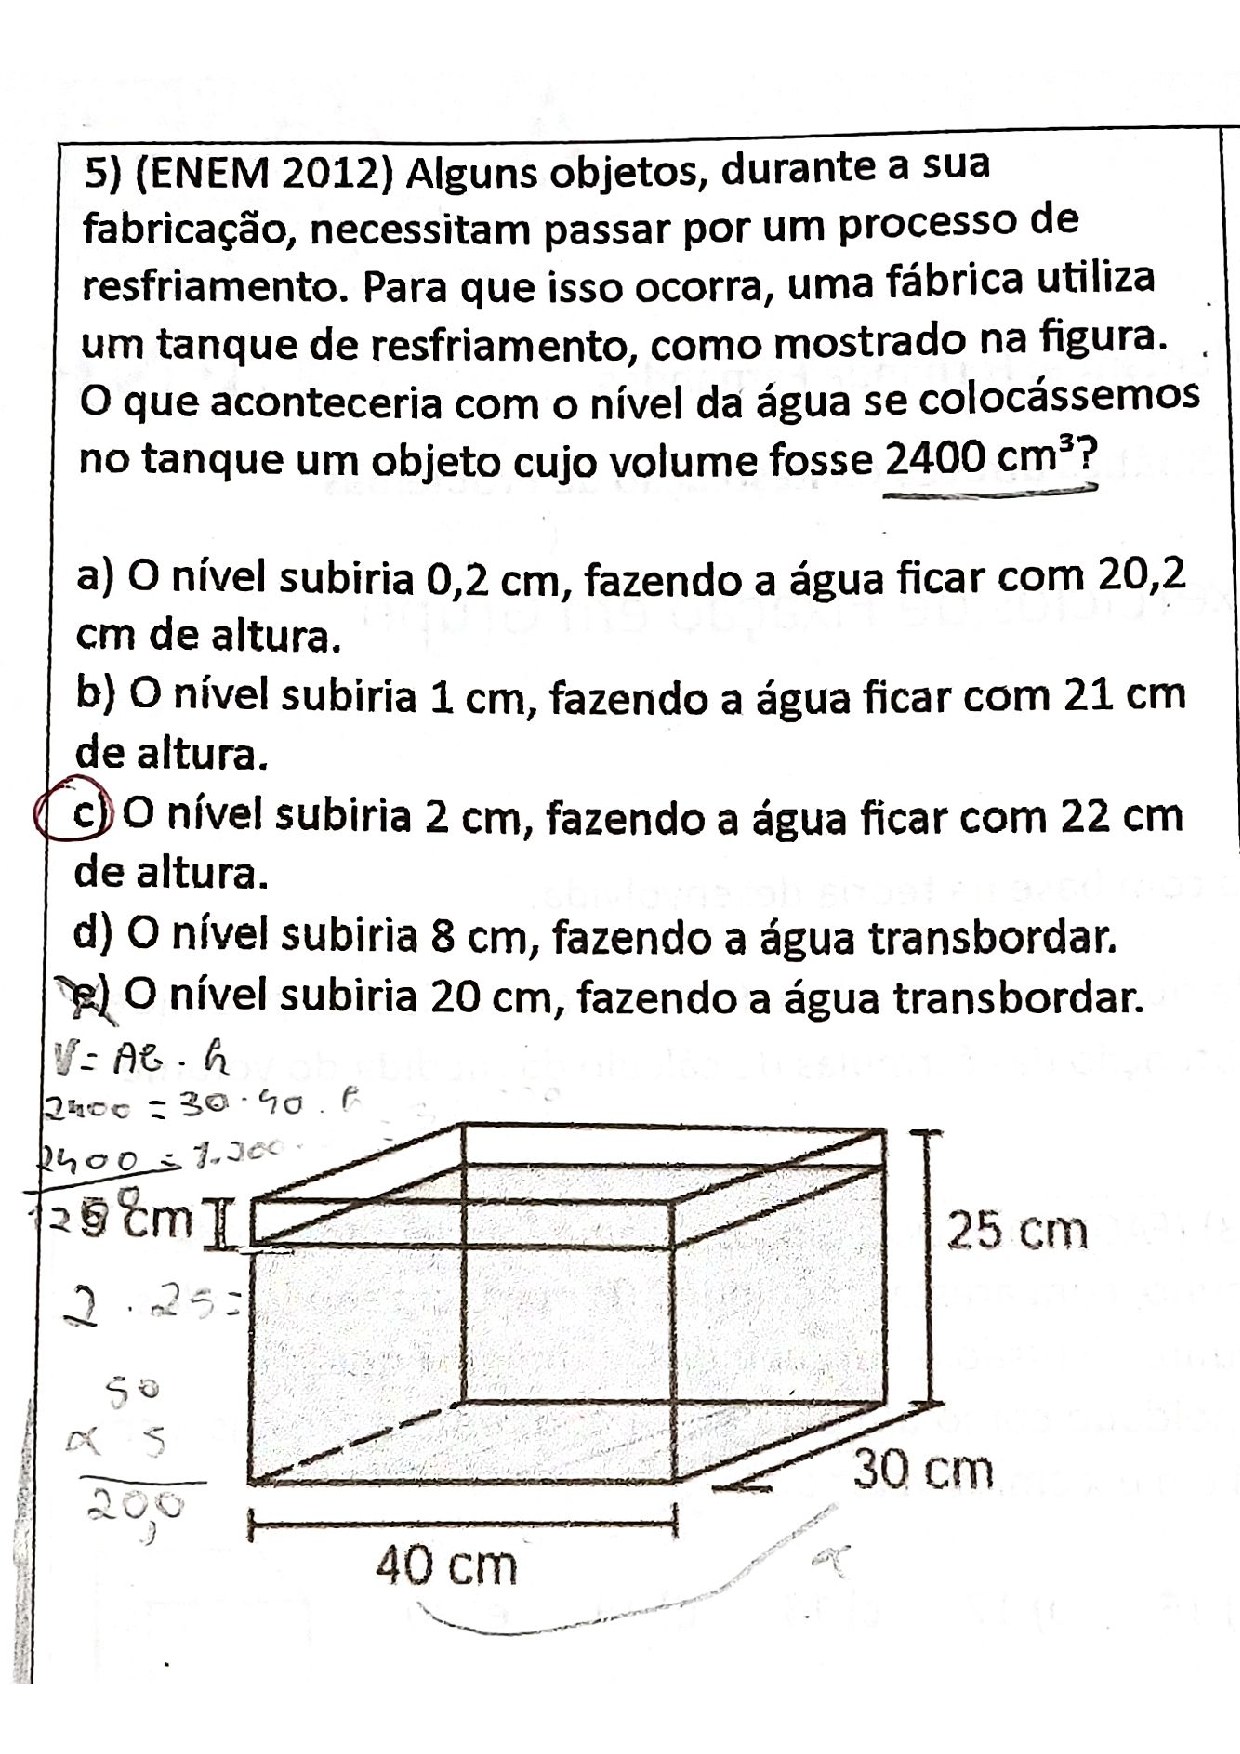
\includegraphics[width=0.5\linewidth]{Novas imagens/254 - Aulas 13 e 14 - Questão 5 - resposta incorreta}
    \legend{\autoria}
\end{CenteredFigure}

\begin{CenteredFigure}
    \caption{Aulas 13 e 14 - Questão 5 - resposta correta} \label{fig: 253 - Aulas 13 e 14 - Questao 5 - resposta correta}
    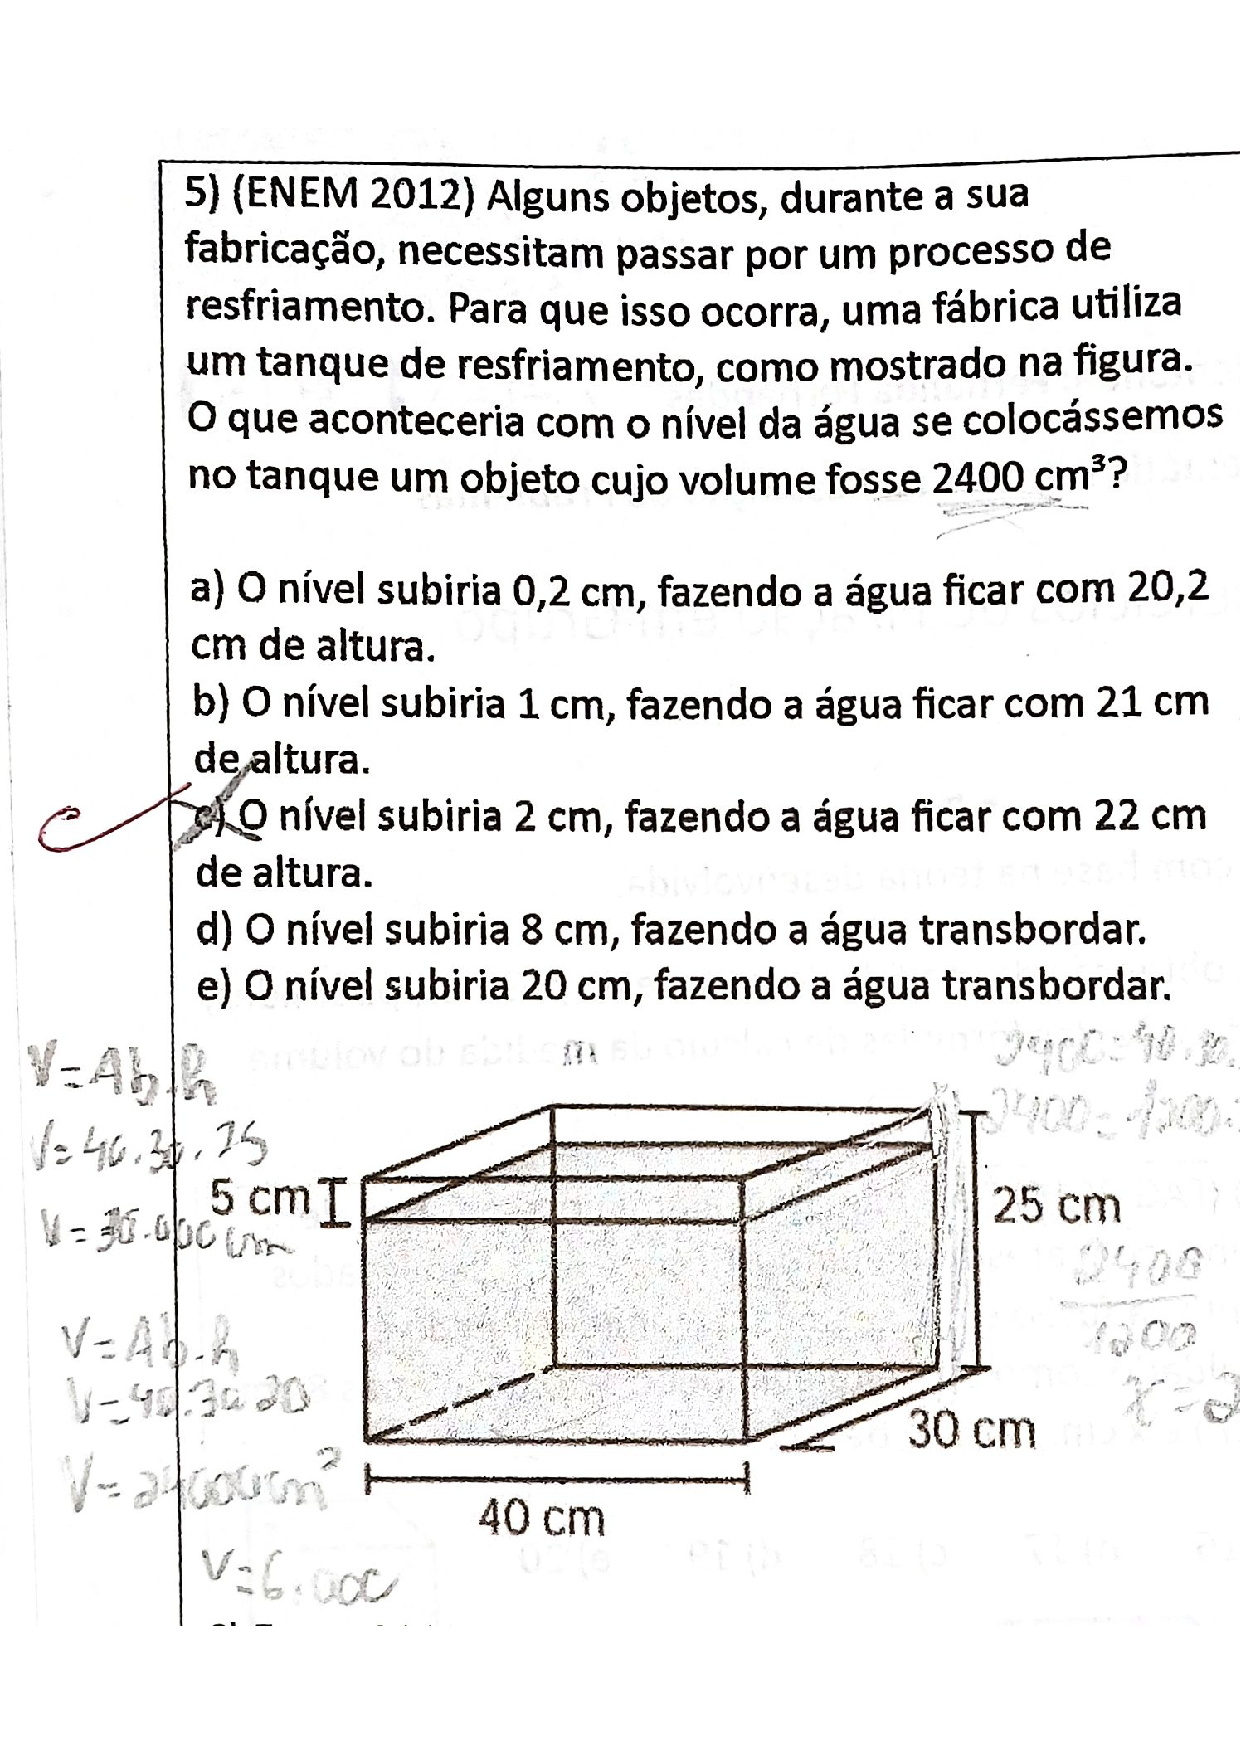
\includegraphics[width=0.5\linewidth]{Novas imagens/253 - Aulas 13 e 14 - Questão 5 - resposta correta}
    \legend{\autoria}
\end{CenteredFigure}

\subsection{Análise das Aulas 15 e 16}

Neste encontro o problema gerador foi: Qual a área lateral e total da pirâmide do seu grupo? A estratégia usada foi calcular a quantidade de papel colorido gasto para cobrir a lateral e a totalidade da superfície da pirâmide (\autoref{ApendiceI}).

Os alunos recortaram, dobraram, colaram e, finalmente, montaram a sua pirâmide (\autoref{fig:10-piramides montadas}). Observaram que, na pirâmide, todas as faces laterais são triângulos e que só possui uma base. Mediram com a régua a base do triângulo e a sua altura. Desenharam e recortaram, no papel laminado, cada face triangular, que foi colada na sua pirâmide (\autoref{fig:11-grupo 1 forrando} e \autoref{fig:12-piramides forradas}).  E, calcularam a quantidade de papel necessária para cobrir uma face da pirâmide. Calcularam a área da base conforme o tipo de pirâmide que receberam. Depois, para calcular a área lateral bastava multiplicar a área de uma face pelo número de lados do polígono da base. E para calcular a área total bastava somar a área da base com a área lateral. Assim, obtiveram a quantidade total de papel laminado necessária para cobrir toda a pirâmide do seu grupo.

Cada grupo apresentou seus cálculos a serem analisados e debatidos na plenária. Em seguida, formalizou-se a área lateral e total da pirâmide.

\textbf{Definição de Pirâmide}: é um poliedro com uma base poligonal e faces laterais que são triângulos, todos convergindo para um ponto chamado vértice. O nome da pirâmide é dado pelo formato de sua base (pirâmide triangular, pirâmide quadrangular).

\textbf{Área Lateral de uma Pirâmide}: é a soma das áreas de todas as suas faces laterais, que são triângulos. Como as laterais são sempre triângulos, a área de uma face é calculada por:

\textcolor[HTML]{0000FF}{$A_L = \left( \frac{b*h}{2}  \right)$}

Onde: a base $b$ de uma face é igual ao lado da base e a altura $h$ igual ao apótema lateral da pirâmide.

No caso particular da base ser um polígono regular:

\textcolor[HTML]{0000FF}{$A_L = n * \left( \frac{b*h}{2}  \right)$}

Onde: $n$ é o número de lados da base e multiplica a área dos triângulos laterais.

\textbf{Área Total de uma Pirâmide}: é a soma da área lateral com a área da base. A fórmula da Área Total é:

\textcolor[HTML]{0000FF}{$AT = A_L + Ab$}

Onde: $A_L$ é a área lateral e $Ab$ é a área da base.

\begin{CenteredFigure}
    \caption{Pirâmides montadas pelos grupos} \label{fig:10-piramides montadas}
    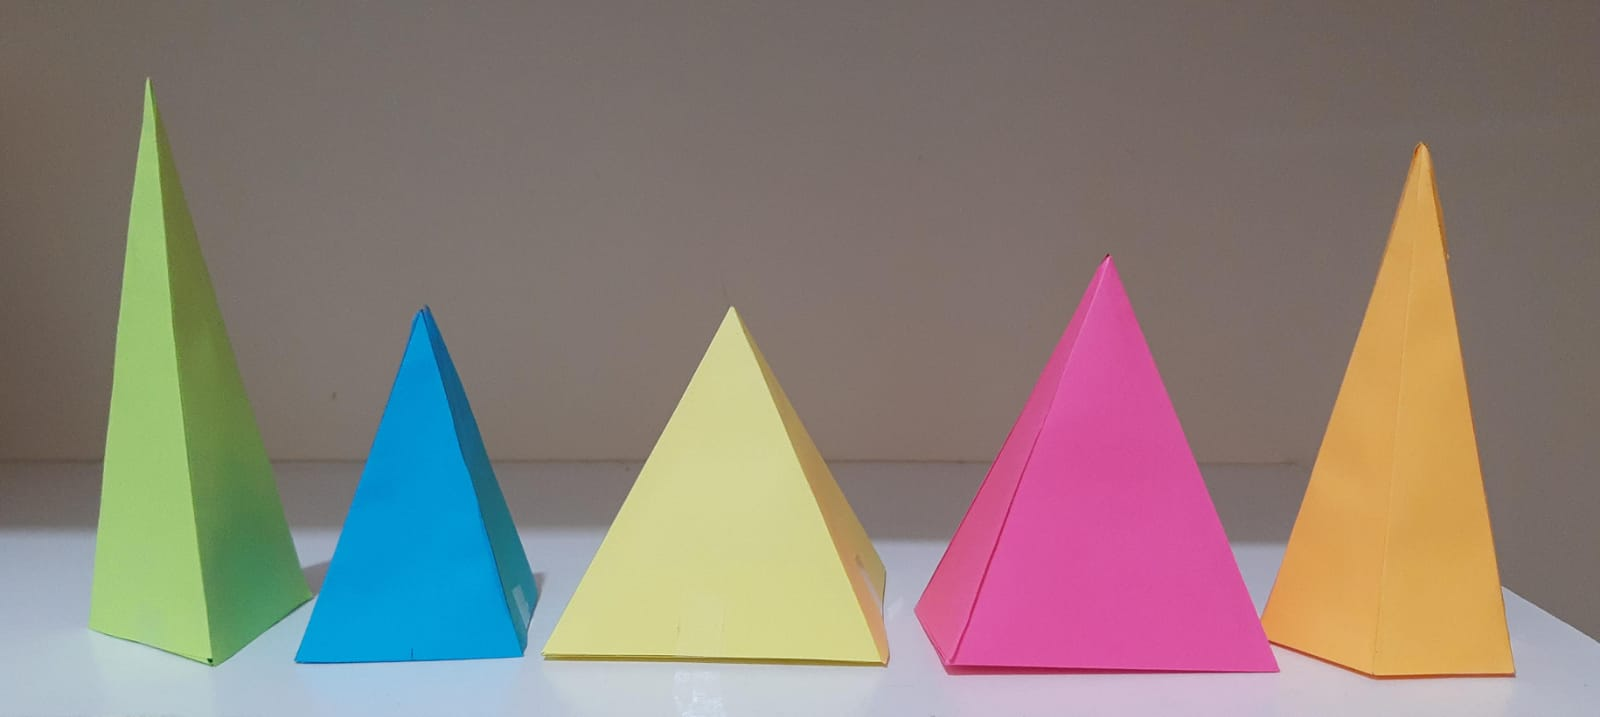
\includegraphics[width=0.5\linewidth]{10-Pirâmides montadas pelos grupos}
    \legend{\autoria}
\end{CenteredFigure}

\begin{CenteredFigure}
    \caption{Forrando a pirâmide quadrangular, estratégia para o cálculo da área lateral e total} \label{fig:11-grupo 1 forrando}
    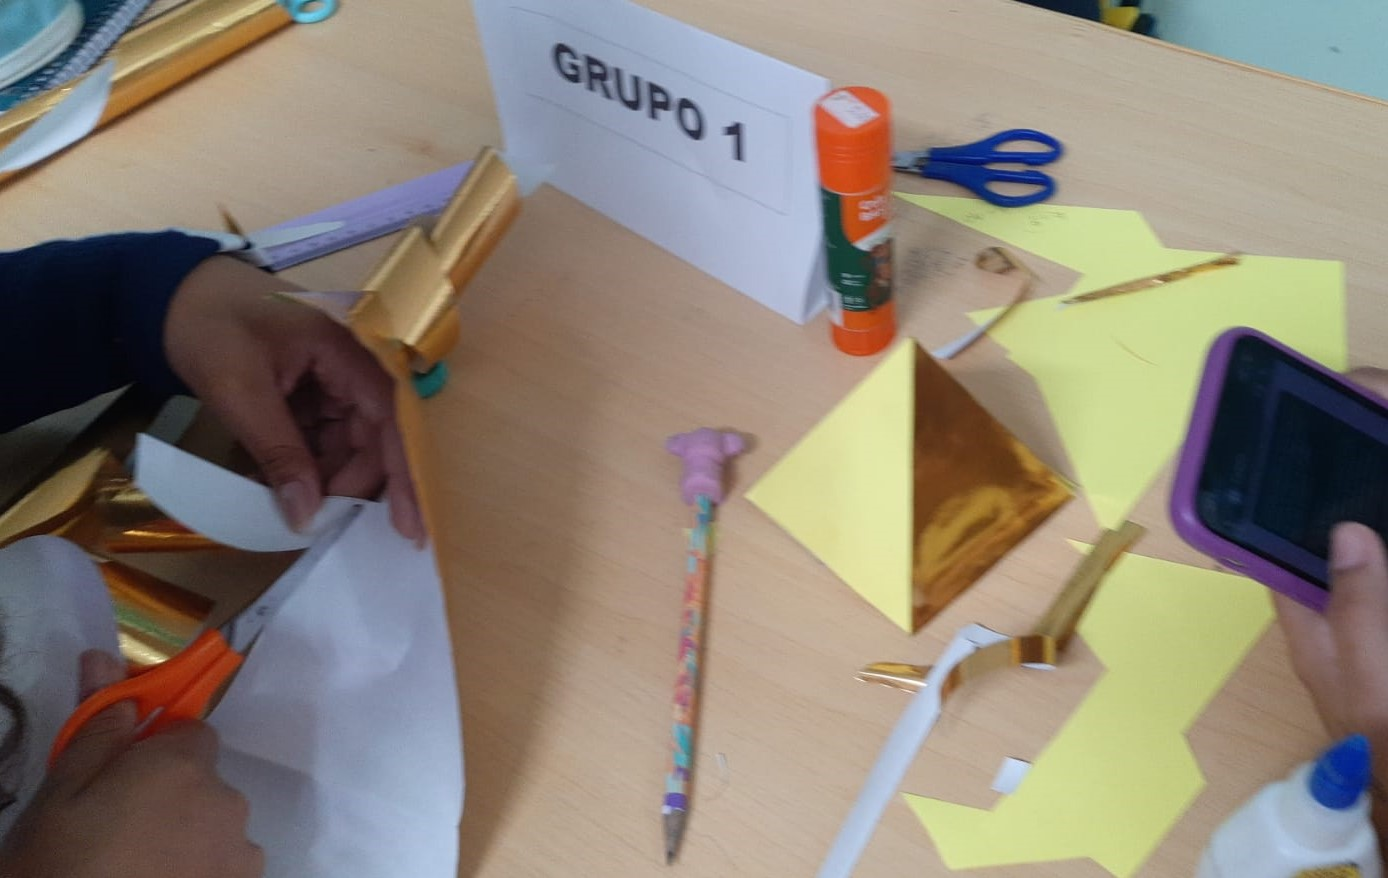
\includegraphics[width=0.5\linewidth]{11-Grupo 1 Pirâmide quadrangular sendo forrada}
    \legend{\autoria}
\end{CenteredFigure}

\begin{CenteredFigure}
    \caption{Pirâmides após o cálculo da área} \label{fig:12-piramides forradas}
    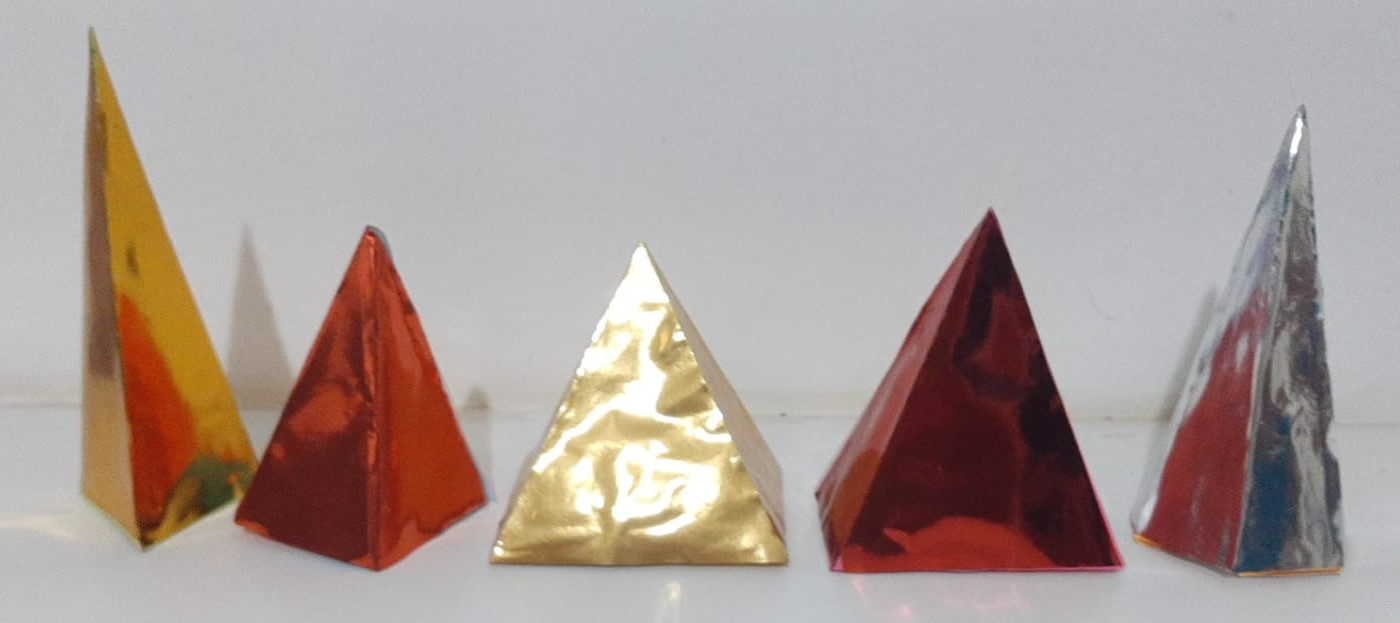
\includegraphics[width=0.5\linewidth]{12-Pirâmides forradas pelos grupos}
    \legend{\autoria}
\end{CenteredFigure}

Este tipo de experimento foi muito apreciado por todos os alunos.

\begin{table}[htbp] \centering
    \caption{Acertos na atividade das aulas 15 e 16} \label{tab:Acertos do Encontro 8}

    \begin{tabular}{|c|c|c|c|c|c|c|}
        \hline
        \textbf{Grupos}       & \textbf{Grupo 1} & \textbf{Grupo 2} & \textbf{Grupo 3} & \textbf{Grupo 4} & \textbf{Grupo 5} \\
        \hline
        Percentual de acertos & 80               & 80               & 70               & 90               & 80               \\
        \hline
    \end{tabular}
    \legend{\legendaTabela}
\end{table}

\subsection{Análise das Aulas 17 e 18}

Nesta aula o objetivo foi: calcular, corretamente, a área lateral e total das pirâmides.

\begin{table}[htbp] \centering
    \caption{Acertos na atividade das aulas 17 e 18} \label{tab:Acertos do Encontro 9}
    \begin{tabular}{|c|c|c|c|c|c|c|}
        \hline
        \textbf{Grupos}       & \textbf{Grupo 1} & \textbf{Grupo 2} & \textbf{Grupo 3} & \textbf{Grupo 4} & \textbf{Grupo 5} \\
        \hline
        Percentual de acertos & 30               & 70               & 90               & 80               & 40               \\
        \hline
    \end{tabular}
    \legend{\legendaTabela}
\end{table}

Iniciou-se fazendo uma recapitulação da definição de a área Lateral e Total das pirâmides e destacando que é muito importante, inicialmente, identificar a base da pirâmide para que se possa calcular, corretamente, a sua área lateral e total. Em seguida, cada grupo recebeu a sua folha de exercícios de fixação do conceito de volume de prisma (\autoref{ApendiceJ}). Cada grupo apresentou sua solução a serem analisadas e debatidas na plenária.

O grupo 1 apresentou certa dificuldade para entender e resolver algumas questões, como mostra a \autoref{tab:Acertos do Encontro 9}. Na \autoref{fig: 255 - Aulas 17 e 18 - Questao 4 - resposta correta} e na \autoref{fig: 256 - Aulas 17 e 18 - Questao 4 - resposta incorreta} temos, respectivamente, a resolução correta e a incorreta da questão 4.

\begin{CenteredFigure}
    \caption{Aulas 17 e 18 - Questão 4 - resposta correta} \label{fig: 255 - Aulas 17 e 18 - Questao 4 - resposta correta}
    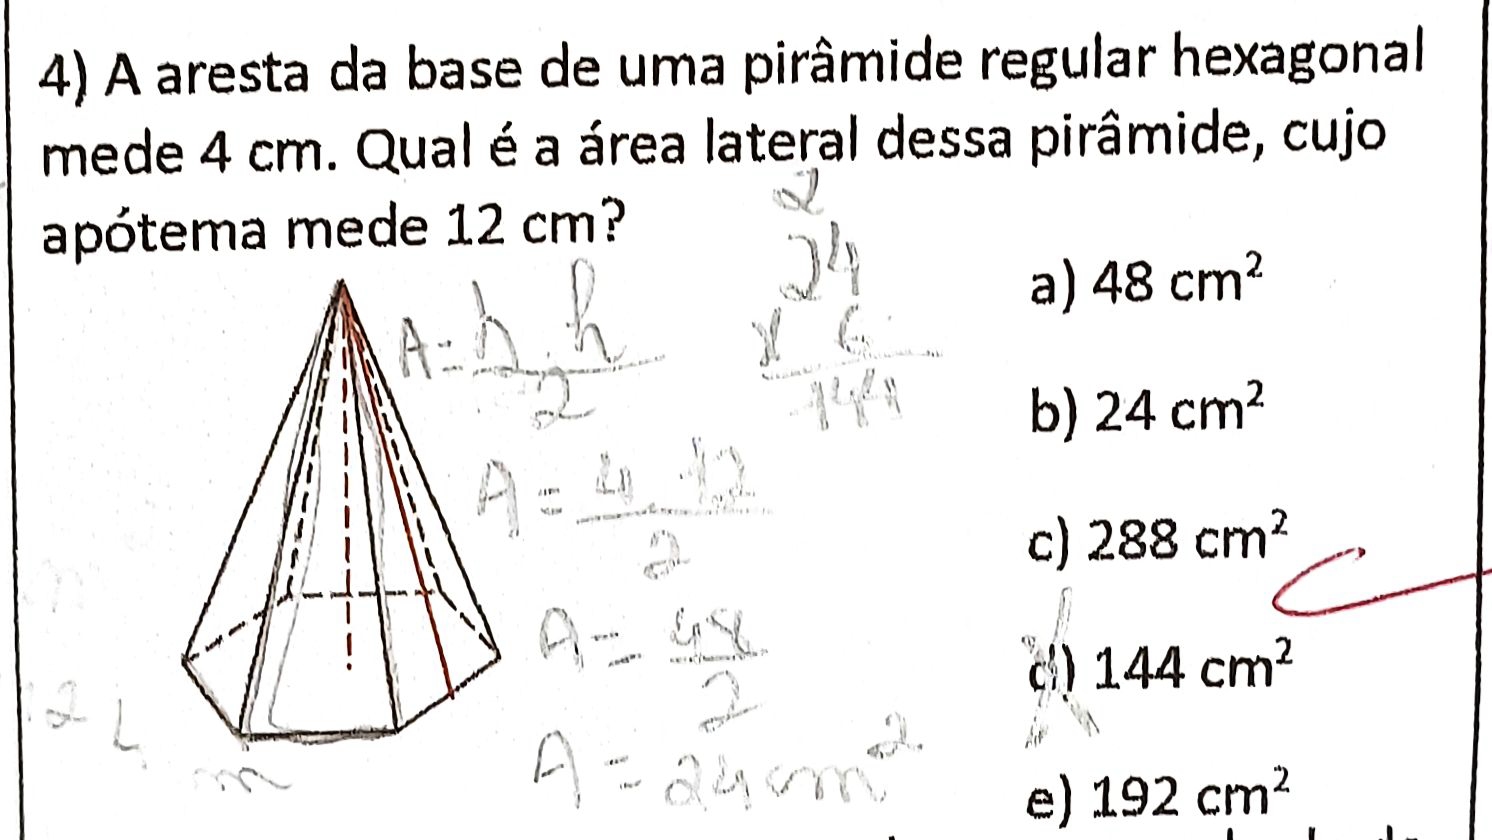
\includegraphics[width=0.4\linewidth]{Novas imagens/255 - Aulas 17 e 18 - Questão 4 - resposta correta}
    \legend{\autoria}
\end{CenteredFigure}

\begin{CenteredFigure}
    \caption{Aulas 17 e 18 - Questão 4 - resposta incorreta} \label{fig: 256 - Aulas 17 e 18 - Questao 4 - resposta incorreta}
    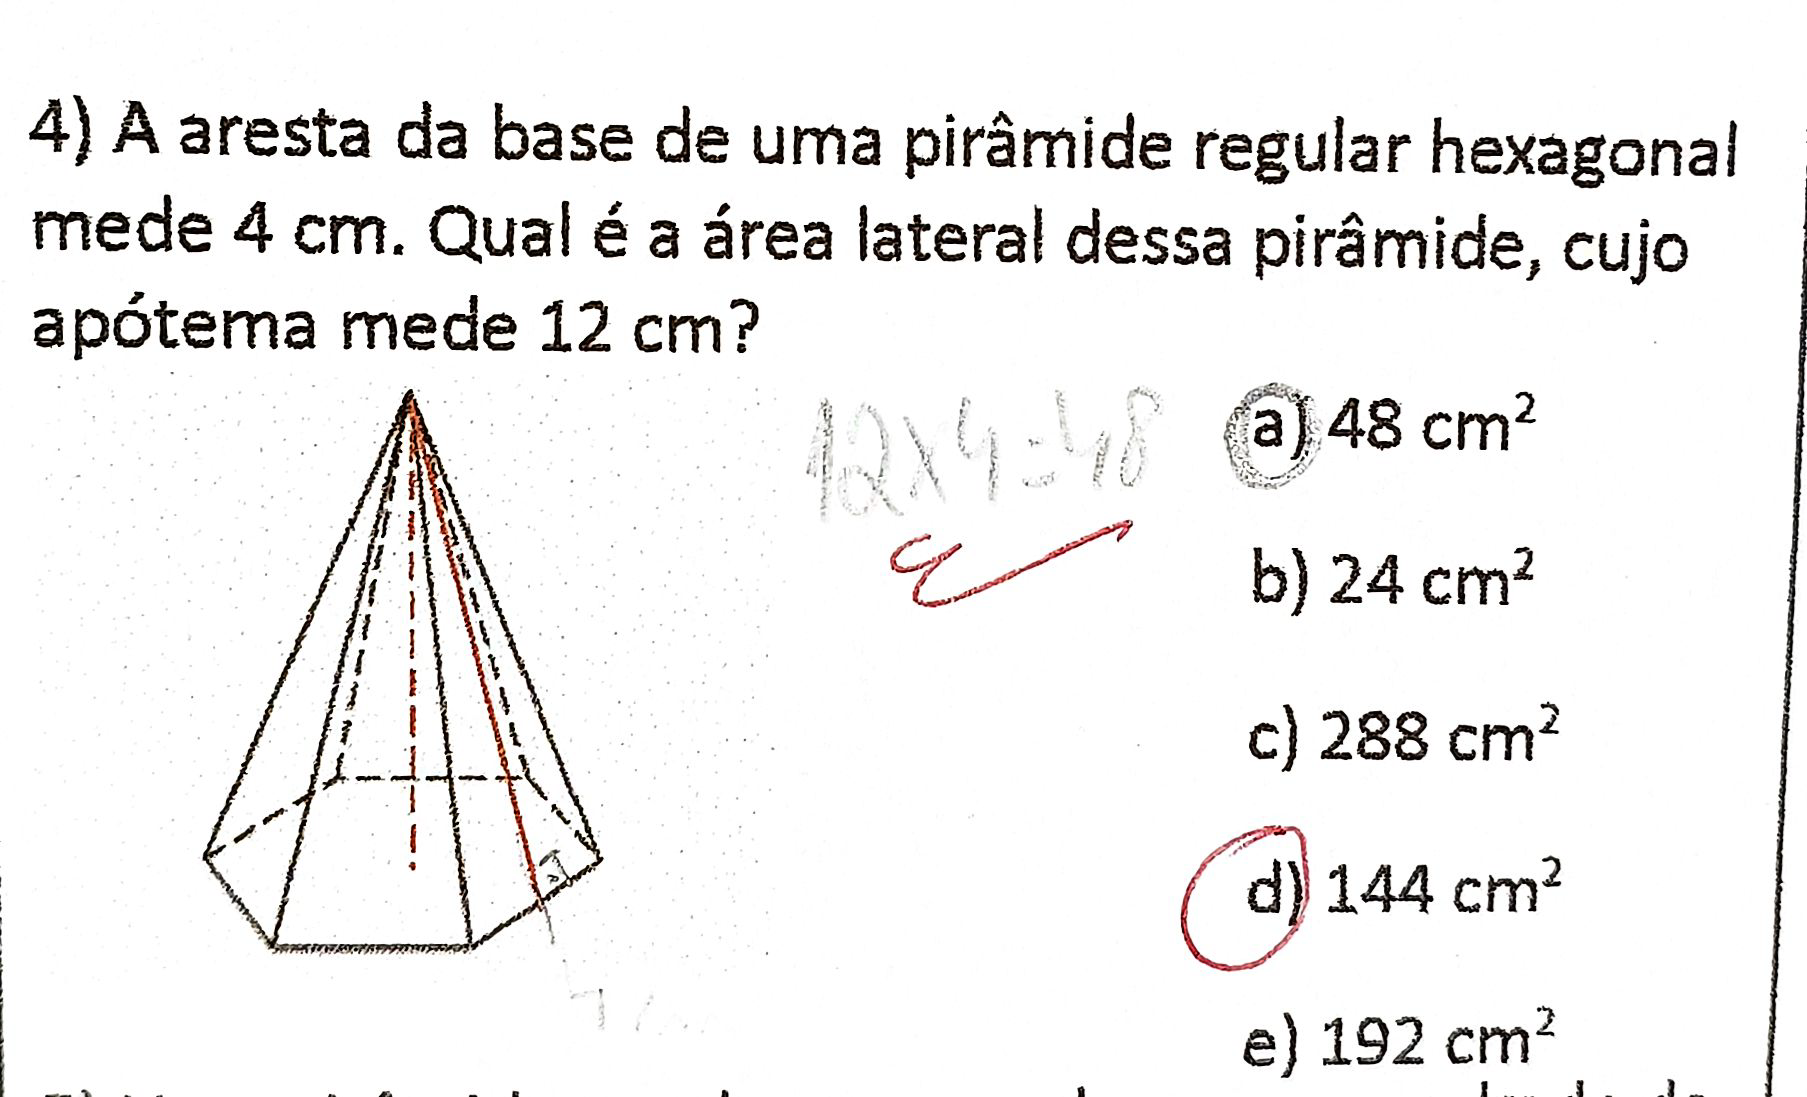
\includegraphics[width=0.4\linewidth]{Novas imagens/256 - Aulas 17 e 18 - Questão 4 - resposta incorreta}
    \legend{\autoria}
\end{CenteredFigure}

\subsection{Análise das Aulas 19 e 20}

Nesta aula cujo objetivo era calcular o volume da pirâmide (\autoref{ApendiceK}). Não foi uma atividade de raciocínio tão imediato.

Como calcular a capacidade da Pirâmide não é tarefa fácil, então, de posse dos grãos triturados, do prisma e da pirâmide, que possuíam a mesma base e a mesma altura (\autoref{fig:14-primas e piramides}), para cada grupo foi solicitado que:

\begin{CenteredFigure}
    \caption{Aulas 19 e 20 - Prismas e pirâmides com mesma base e mesma altura} \label{fig:14-primas e piramides}
    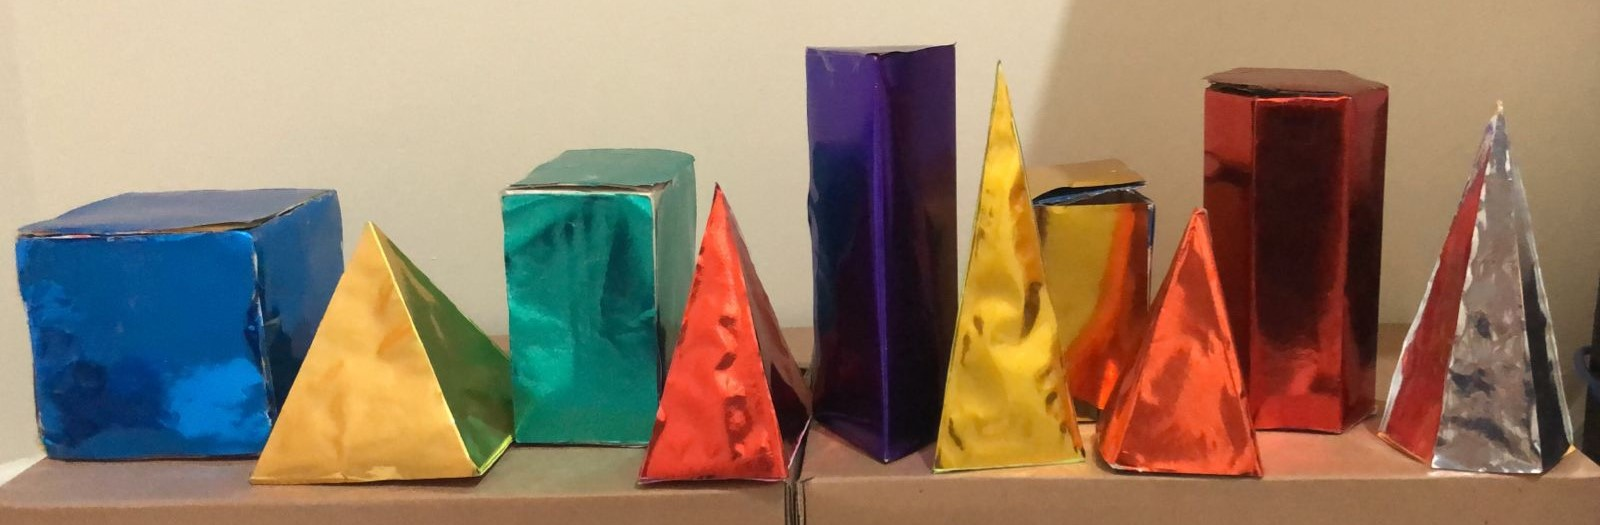
\includegraphics[width=0.5\linewidth]{14-Prisma e Pirâmide de cada grupo}
    \legend{\autoria}
\end{CenteredFigure}

\begin{CenteredFigure}
    \caption{Medindo o volume} \label{fig:15-Aulas 19 e 20 - Medindo o volume}
    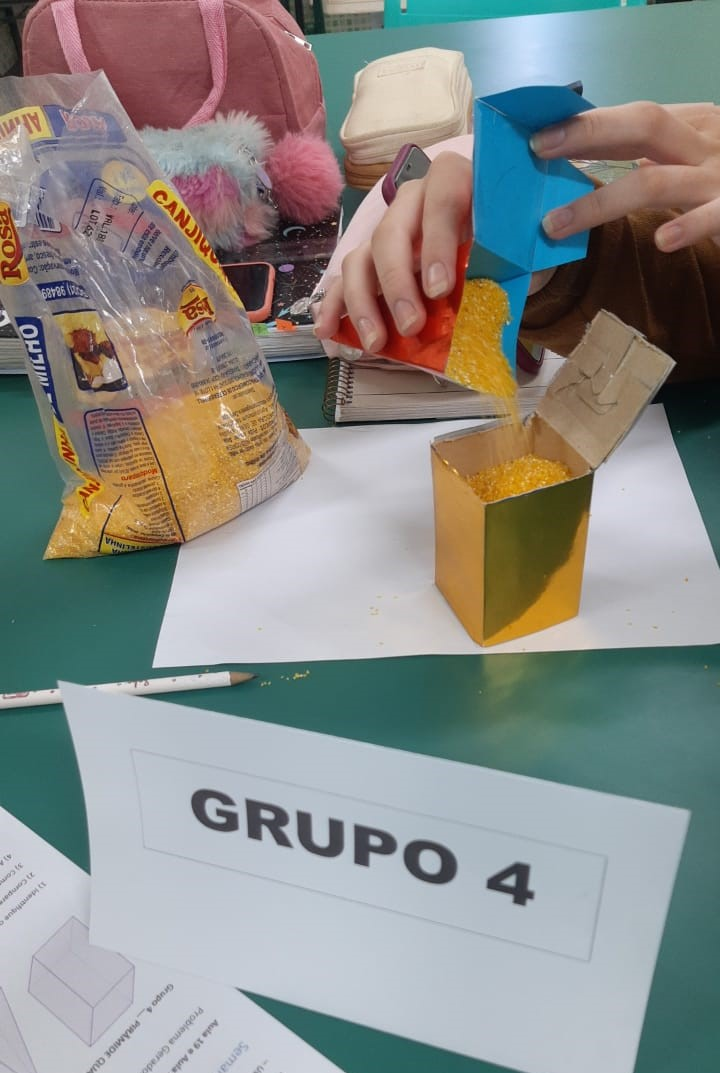
\includegraphics[width=0.5\linewidth]{15-Grupo 4 enchendo o prisma quadrangular}
    \legend{\autoria}
\end{CenteredFigure}

\begin{enumerate}
    \item Identificasse os poliedros que receberam;
    \item Comparasse a altura dos 2 poliedros que receberam;
    \item Comparasse as bases dos 2 poliedros que receberam;
    \item Abrisse apenas uma base do prisma e a base da pirâmide;
    \item Enchesse totalmente o seu prisma, usando a sua pirâmide como medidor, observando quantas desse medidor são necessários para enchê-lo completamente.
\end{enumerate}

A partir deste experimento (\autoref{fig:15-Aulas 19 e 20 - Medindo o volume}), os grupos apresentaram os resultados encontrados e, na plenária, concluiu-se que, todos os grupos precisaram do conteúdo de 3 pirâmides/medidor para encher, completamente, o prisma correspondente e que o volume da pirâmide é um terço da área da base vezes a sua altura.

Em seguida, após a plenária formalizou-se a definição do volume da pirâmide:

\textbf{Definição de Volume de uma Pirâmide}: é a quantidade de espaço tridimensional que a pirâmide ocupa. Ele é calculado multiplicando-se a área da base pela altura da pirâmide e, em seguida, dividindo o resultado por três. Isso ocorre porque a pirâmide ocupa apenas um terço do volume de um prisma com a mesma base e altura.

\textbf{Fórmula do Volume de uma Pirâmide} é \textcolor[HTML]{0000FF}{$V = \frac{Ab *H}{3}$}, onde $V$ é o volume da pirâmide, $Ab$ é a área da base da pirâmide e $H$ é a altura da pirâmide.

Este tipo de experimento foi muito encantador para os alunos! E a aprendizagem foi satisfatória como mostra a \autoref{tab:Acertos do Encontro 10}.

\begin{table}[htbp] \centering
    \caption{Acertos na atividade das aulas 19 e 20} \label{tab:Acertos do Encontro 10}
    \begin{tabular}{|c|c|c|c|c|c|c|}
        \hline
        \textbf{Grupos}       & \textbf{Grupo 1} & \textbf{Grupo 2} & \textbf{Grupo 3} & \textbf{Grupo 4} & \textbf{Grupo 5} \\
        \hline
        Percentual de acertos & 100              & 100              & 100              & 100              & 100              \\
        \hline
    \end{tabular}
    \legend{\legendaTabela}
\end{table}

\subsection{Análise das Aulas 21 e 22}

Neste encontro a proposta foi a resolução dos exercícios para fixar o conceito de Volume de Pirâmides (\autoref{ApendiceL}), cujo objetivo é: calcular, corretamente, o volume das pirâmides.

Para fixar esses conceitos, é essencial praticar com exercícios que envolvam diferentes formas de bases e alturas das pirâmides. Isso ajuda a consolidar a compreensão da relação entre a área da base, a altura e o volume nas diferentes figuras geométricas.

% Como mostra a \autoref{fig:16-grupo 5 resolucao}.

% \begin{CenteredFigure}
%     \caption{Grupo 5 apresentando sua resolução} \label{fig:16-grupo 5 resolucao}
%     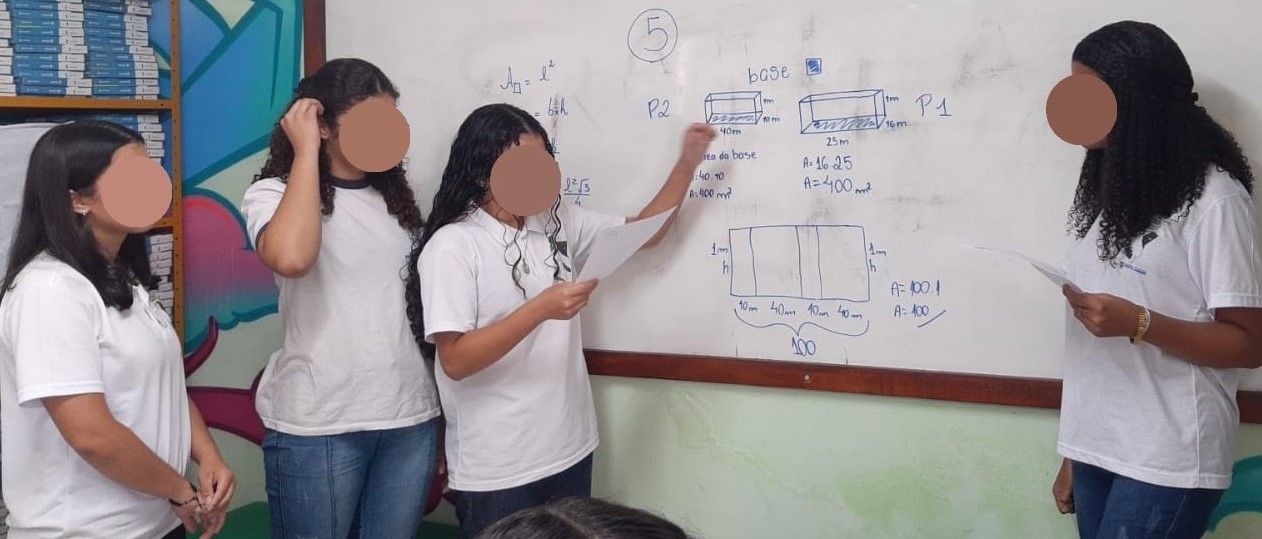
\includegraphics[width=0.5\linewidth]{16-Grupo 5 - Apresentando seus cálculos}
%     \legend{\autoria}
% \end{CenteredFigure}

Percebeu-se que, o grupo 2 apresentou certa dificuldade para entender e resolver algumas questões, como mostra a \autoref{tab:Acertos do Encontro 11} e a \autoref{fig: 257 - Aulas 21 e 22 - Questao 1 - resposta incorreta}. E, na \autoref{fig: 258 - Aulas 21 e 22 - Questao 1 - resposta correta}, constata-se o cálculo correto da mesma questão, feito pelo grupo 5.

\begin{table}[htbp] \centering
    \caption{Acertos na atividade das aulas 21 e 22} \label{tab:Acertos do Encontro 11}
    \begin{tabular}{|c|c|c|c|c|c|c|}
        \hline
        \textbf{Grupos}       & \textbf{Grupo 1} & \textbf{Grupo 2} & \textbf{Grupo 3} & \textbf{Grupo 4} & \textbf{Grupo 5} \\
        \hline
        Percentual de acertos & 75               & 50               & 80               & 100              & 100              \\
        \hline
    \end{tabular}
    \legend{\legendaTabela}
\end{table}

\begin{CenteredFigure}
    \caption{Aulas 21 e 22 - Questão 1 - cálculo incorreto} \label{fig: 257 - Aulas 21 e 22 - Questao 1 - resposta incorreta}
    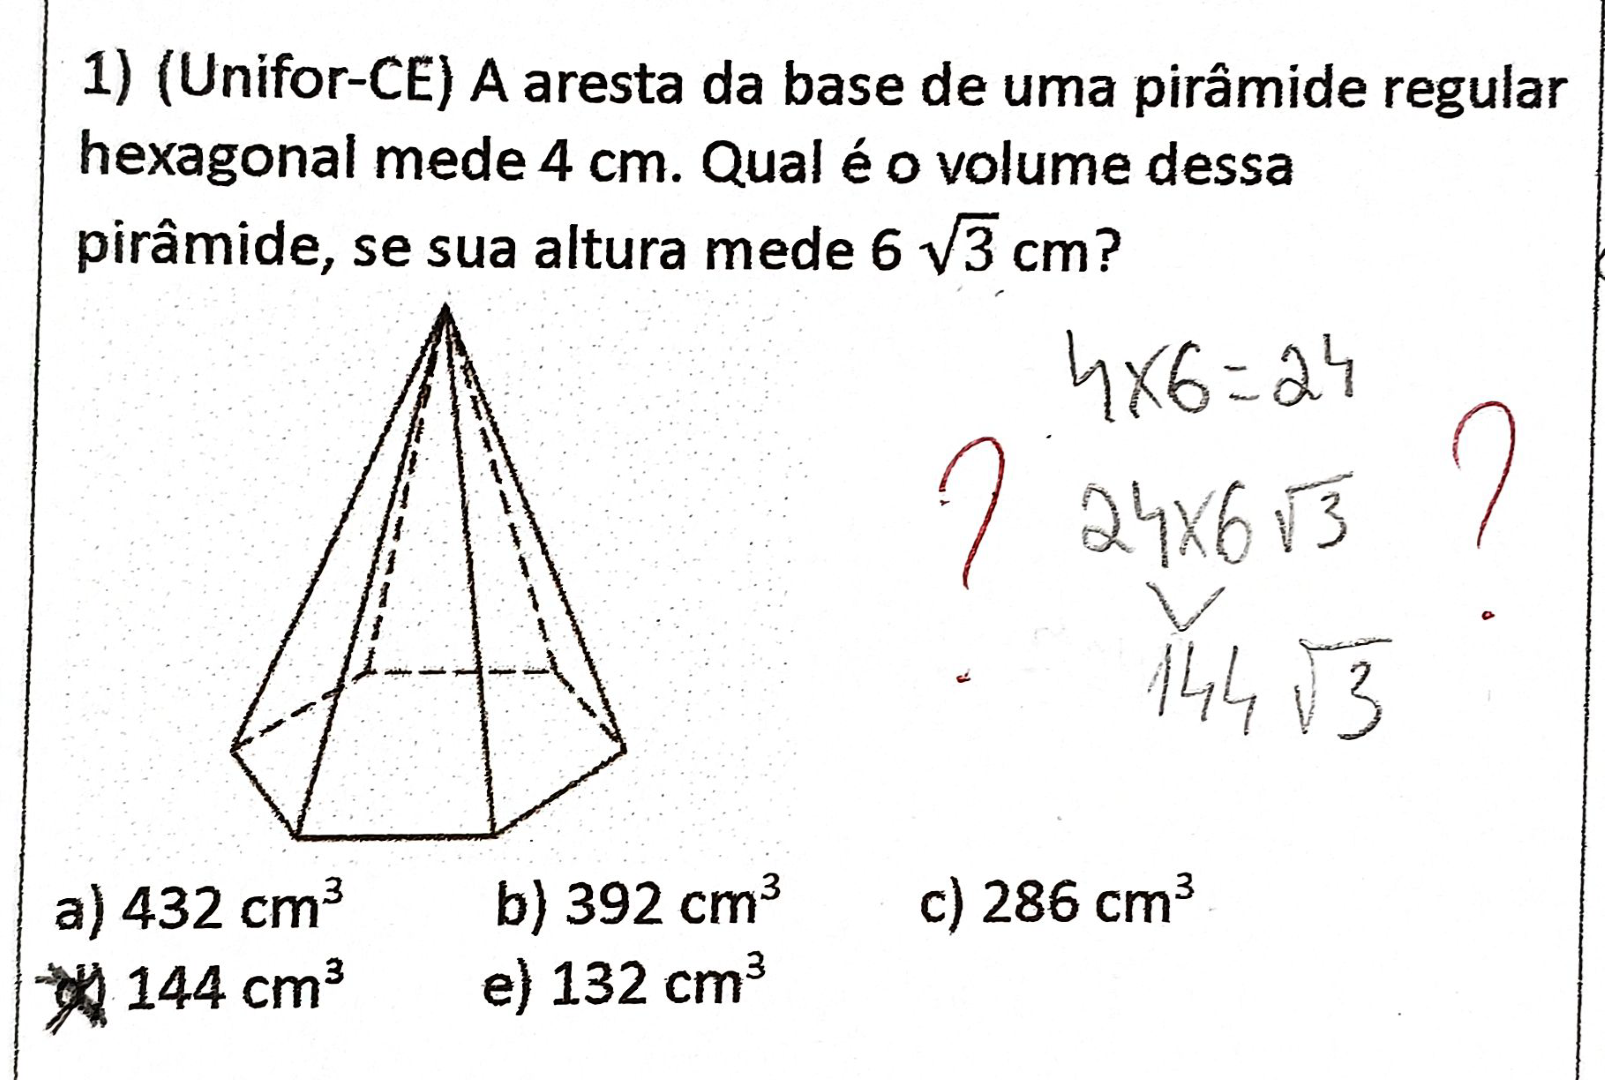
\includegraphics[width=0.5\linewidth]{Novas imagens/257 - Aulas 21 e 22 - Questão 1 - resposta incorreta}
    \legend{\autoria}
\end{CenteredFigure}

\begin{CenteredFigure}
    \caption{Aulas 21 e 22 - Questão 1 - cálculo e resposta corretos} \label{fig: 258 - Aulas 21 e 22 - Questao 1 - resposta correta}
    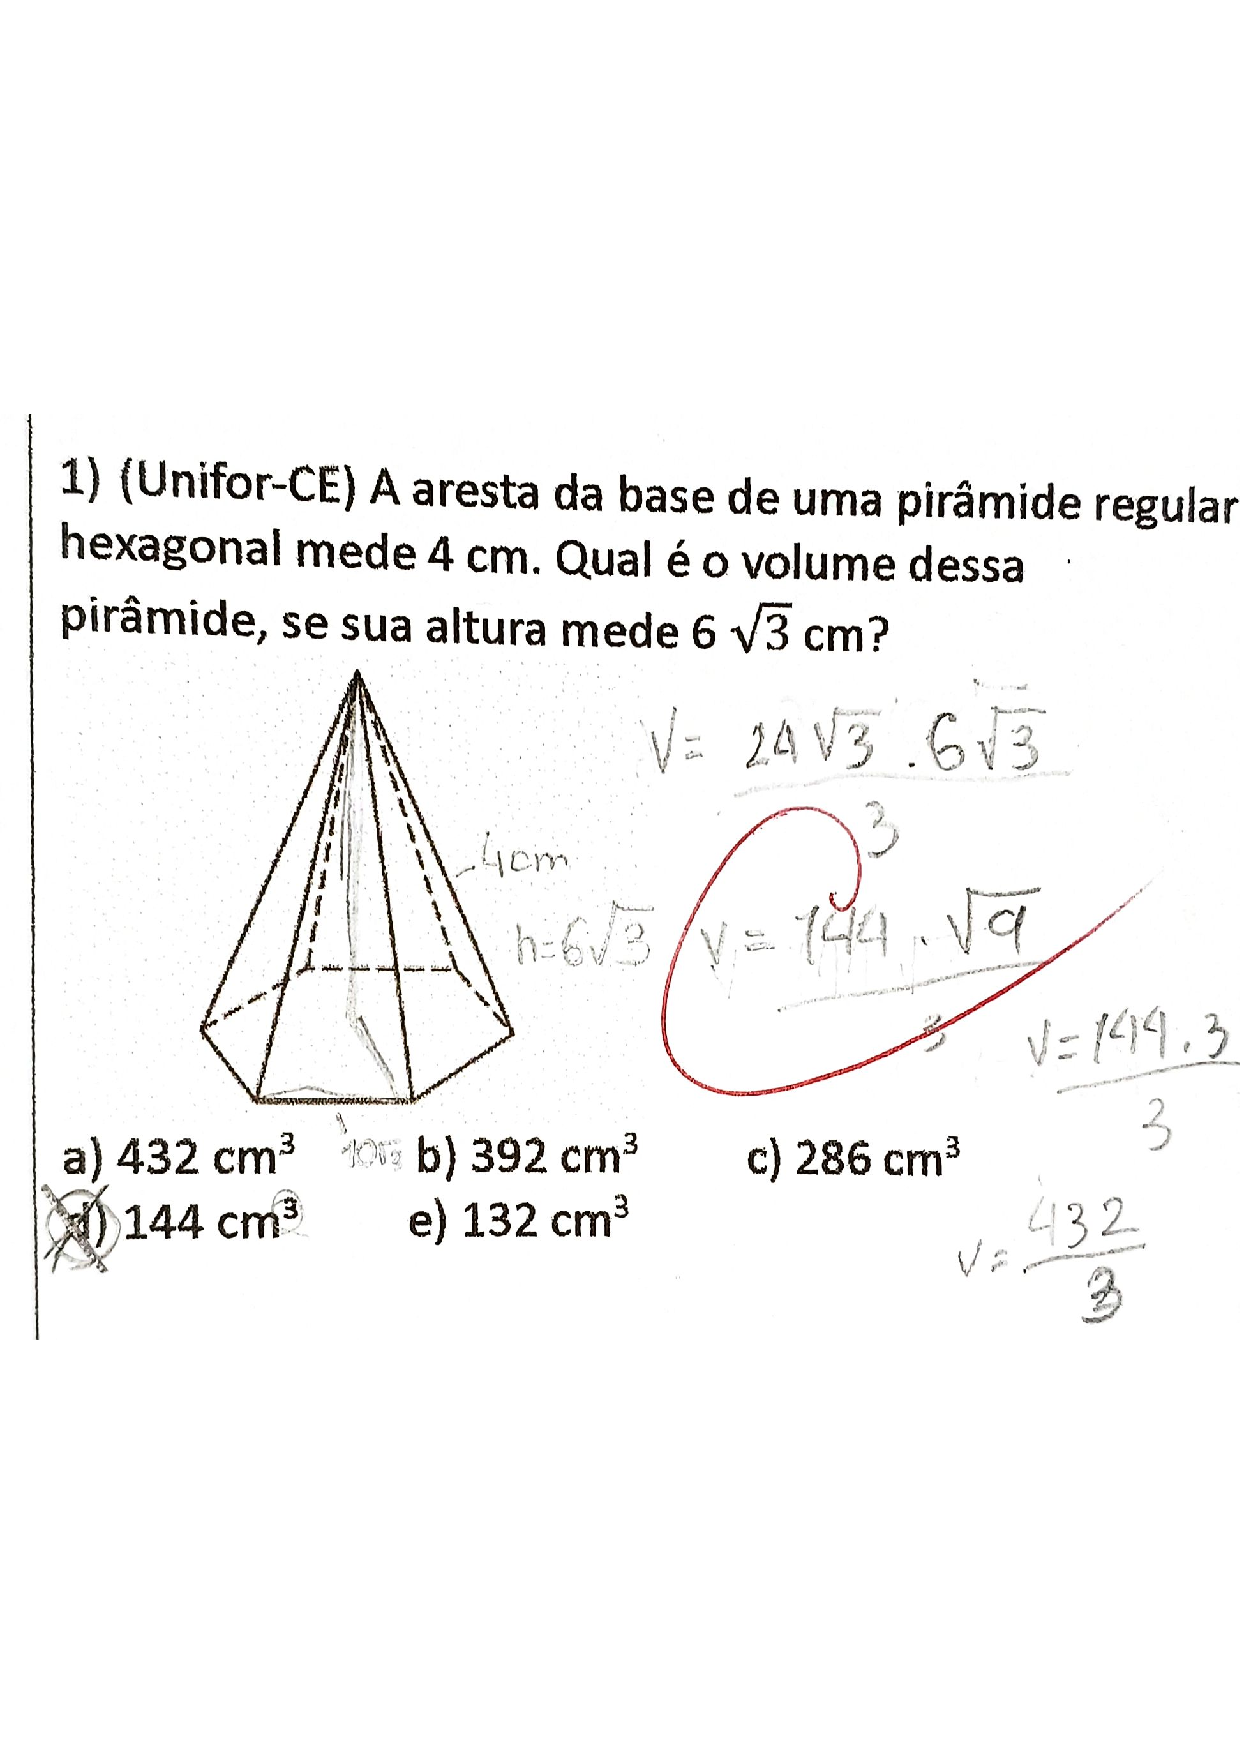
\includegraphics[width=0.5\linewidth]{Novas imagens/258 - Aulas 21 e 22 - Questão 1 - resposta correta}
    \legend{\autoria}
\end{CenteredFigure}

\subsection{Análise das Aulas 23 e 24}

A avaliação holística, onde avaliou-se o ensino-aprendizagem usando-se como estratégia a Confecção de um Álbum de Figurinhas sobre Poliedros (\autoref{ApendiceM}), visando considerar o indivíduo de maneira integral. Isso significa avaliar não apenas o conhecimento teórico, mas também habilidades práticas, criativas e sociais.

Foi incrível observar que cada aluno, intuitivamente, usou um recurso diferente para facilitar a identificação correta da figura que ocuparia determinado espaço e que não mais poderia ser usada outra vez. Alguns separaram por página, outros desenharam a figura no espaço do álbum (\autoref{fig:17-estretegia de desenhar}), outros numeraram e reproduziram as planificações (\autoref{fig:18-estrategia de reproduzir}), outros numeraram o verso da figura (\autoref{fig:19-estrategia de numerar}) e outros colocaram o nome na figura.

\begin{CenteredFigure}
    \caption{Aulas 23 e 24 - Estratégia de desenhar o sólido} \label{fig:17-estretegia de desenhar}
    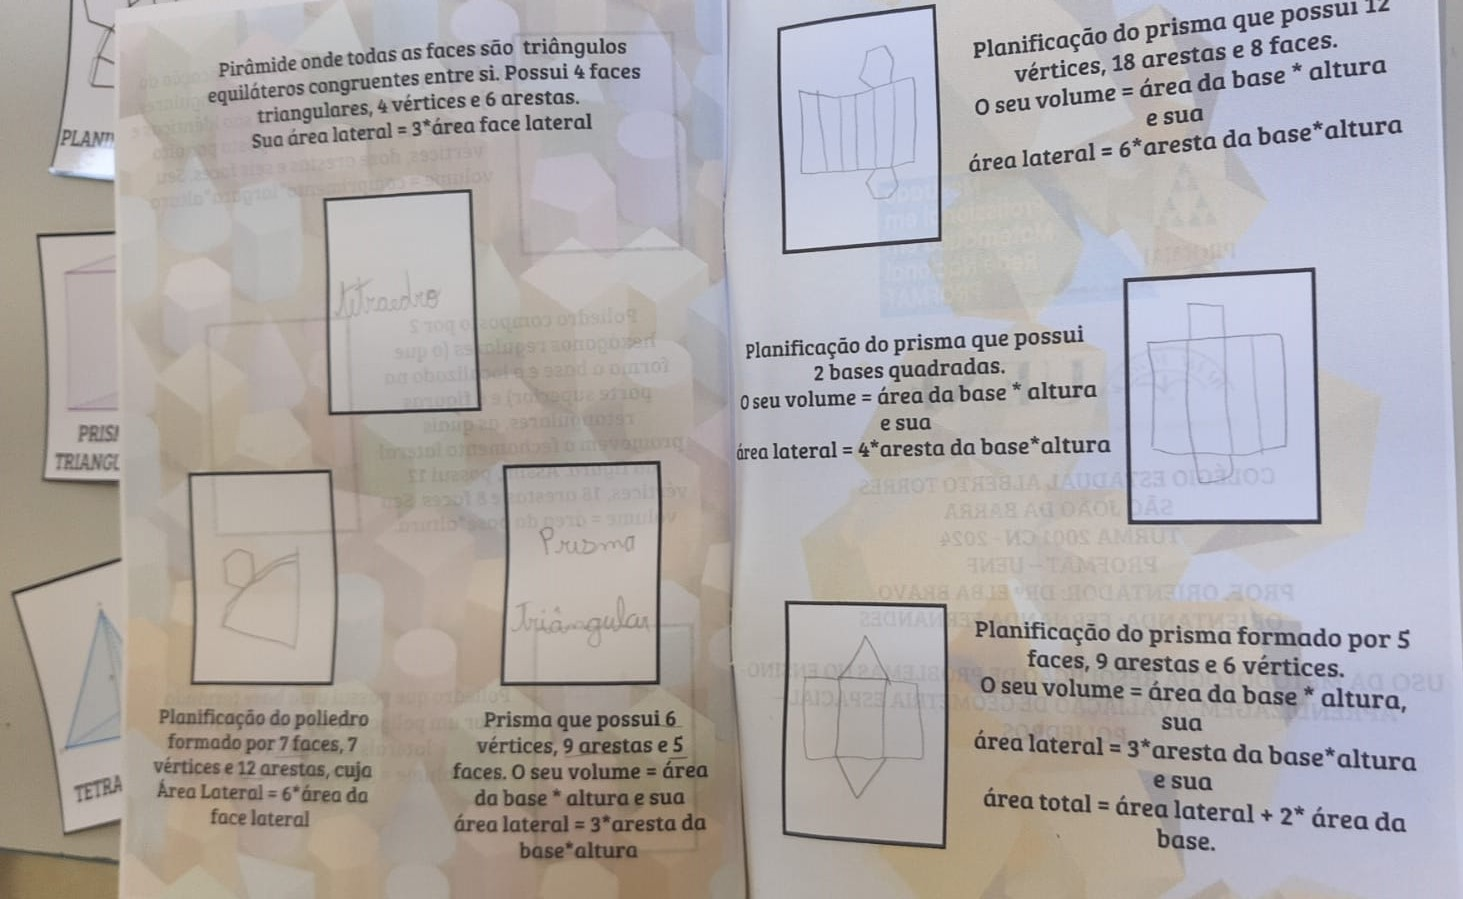
\includegraphics[width=0.5\linewidth]{17-Estratégia de desenhar a figurinha}
    \legend{\autoria}
\end{CenteredFigure}

\begin{CenteredFigure}
    \caption{Aulas 23 e 24 - Estratégia de numerar e reproduzir planificações} \label{fig:18-estrategia de reproduzir}
    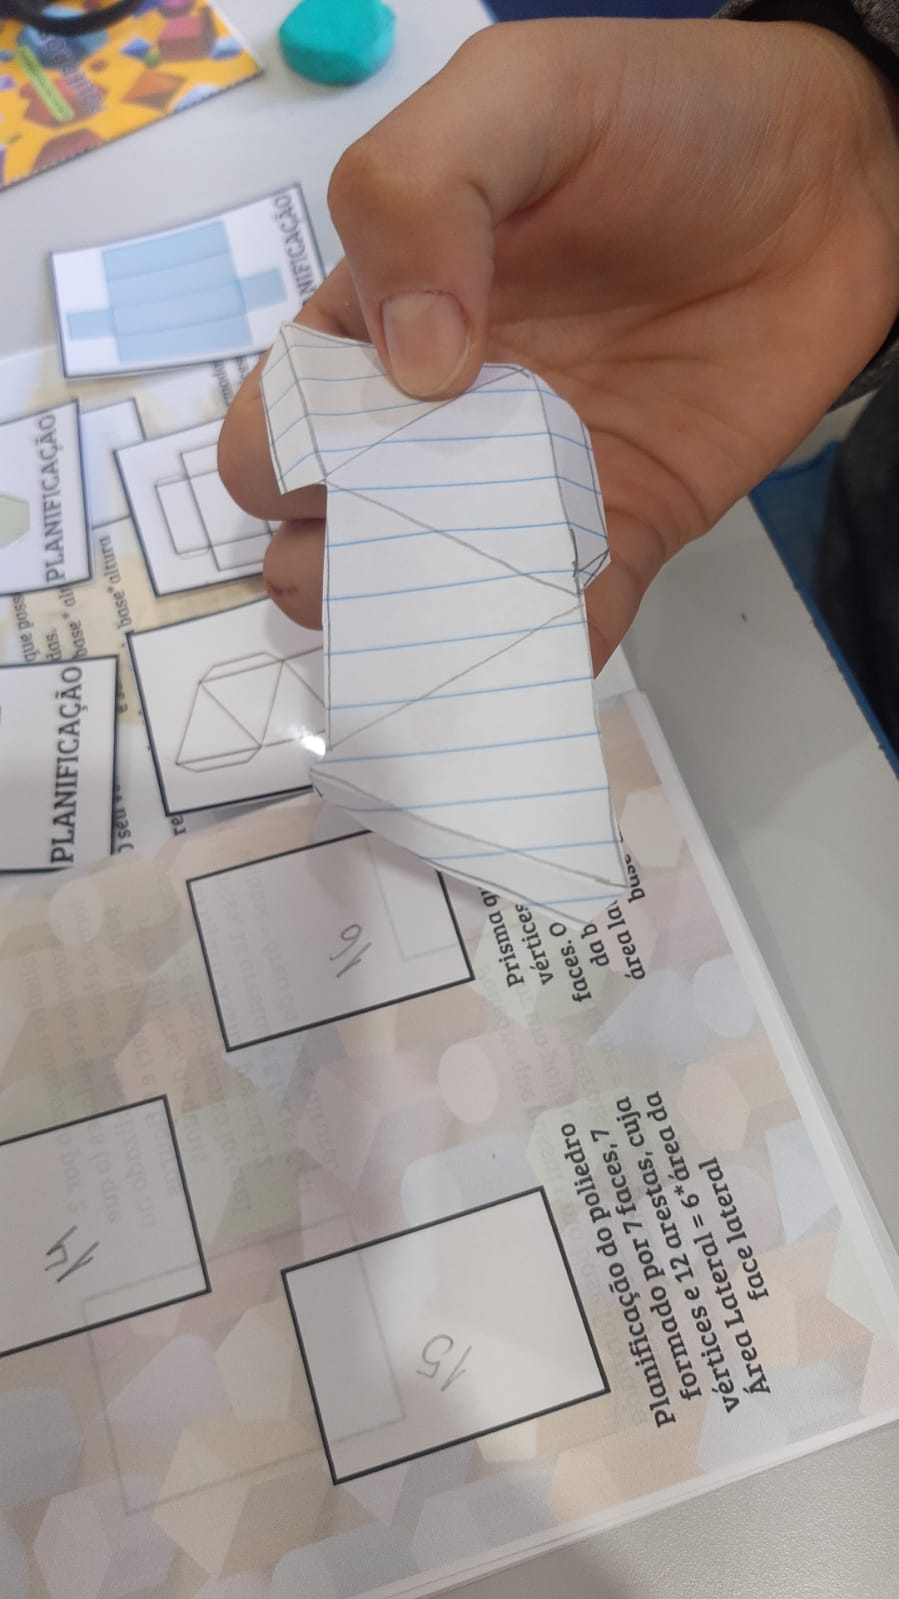
\includegraphics[width=0.5\linewidth]{18-Estratégia de numerar e reproduzir planificações}
    \legend{\autoria}
\end{CenteredFigure}

\begin{CenteredFigure}
    \caption{Aulas 23 e 24 - Estratégia de numerar} \label{fig:19-estrategia de numerar}
    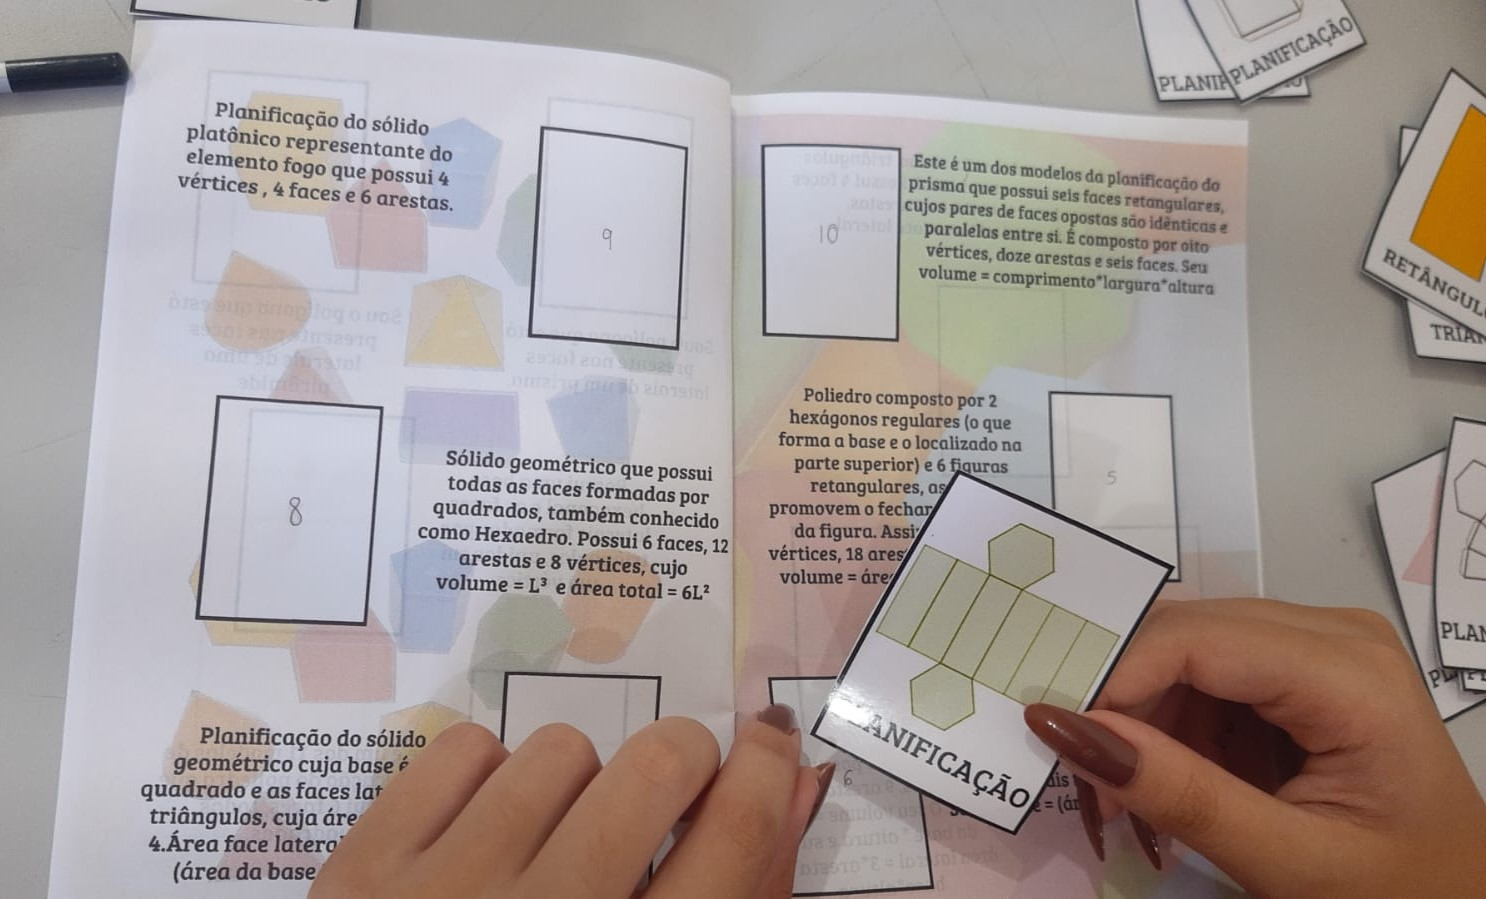
\includegraphics[width=0.5\linewidth]{19-Estratégia de numerar I}
    \legend{\autoria}
\end{CenteredFigure}

\begin{CenteredFigure}
    \caption{Aulas 23 e 24 - Colagem incorreta no Álbum de Figurinhas} \label{fig: 259 - Aulas 23 e 24 - Colagem incorreta no Album de Figurinhas}
    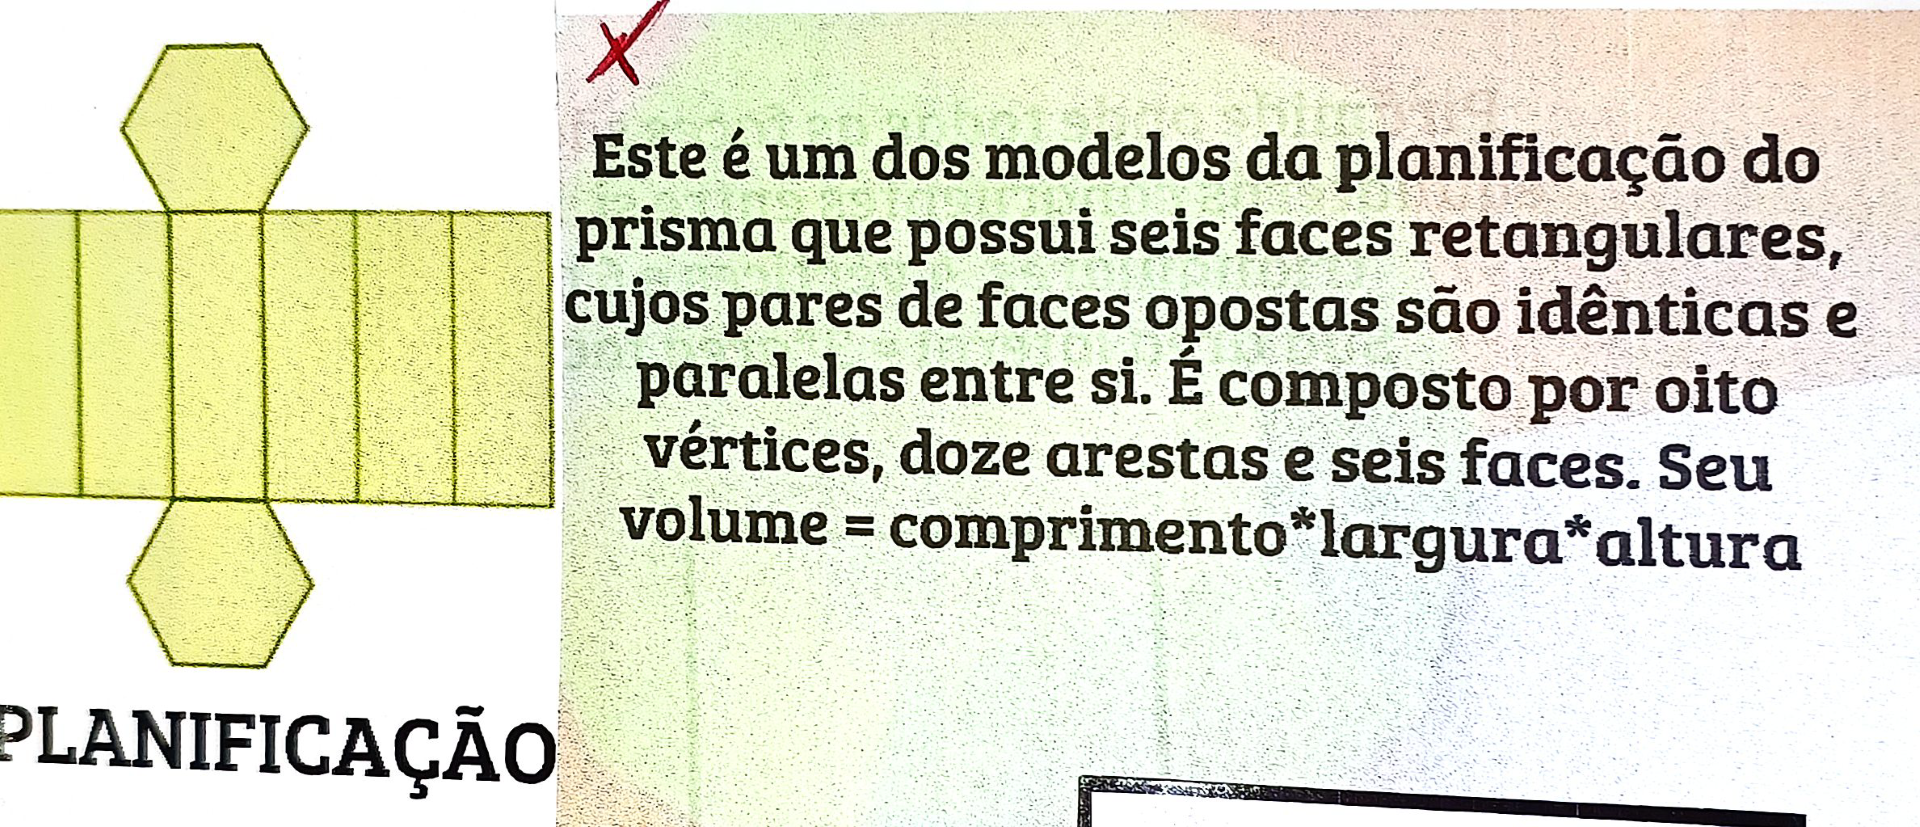
\includegraphics[width=0.5\textwidth]{Novas imagens/259 - Aulas 23 e 24 - Colagem incorreta no Álbum de Figurinhas}
    \legend{\autoria}
\end{CenteredFigure}

\begin{CenteredFigure}
    \caption{Aulas 23 e 24 - Colagem incorreta no Álbum de Figurinhas} \label{fig: 261 - Aulas 23 e 24 - Colagem incorreta no Album de Figurinhas}
    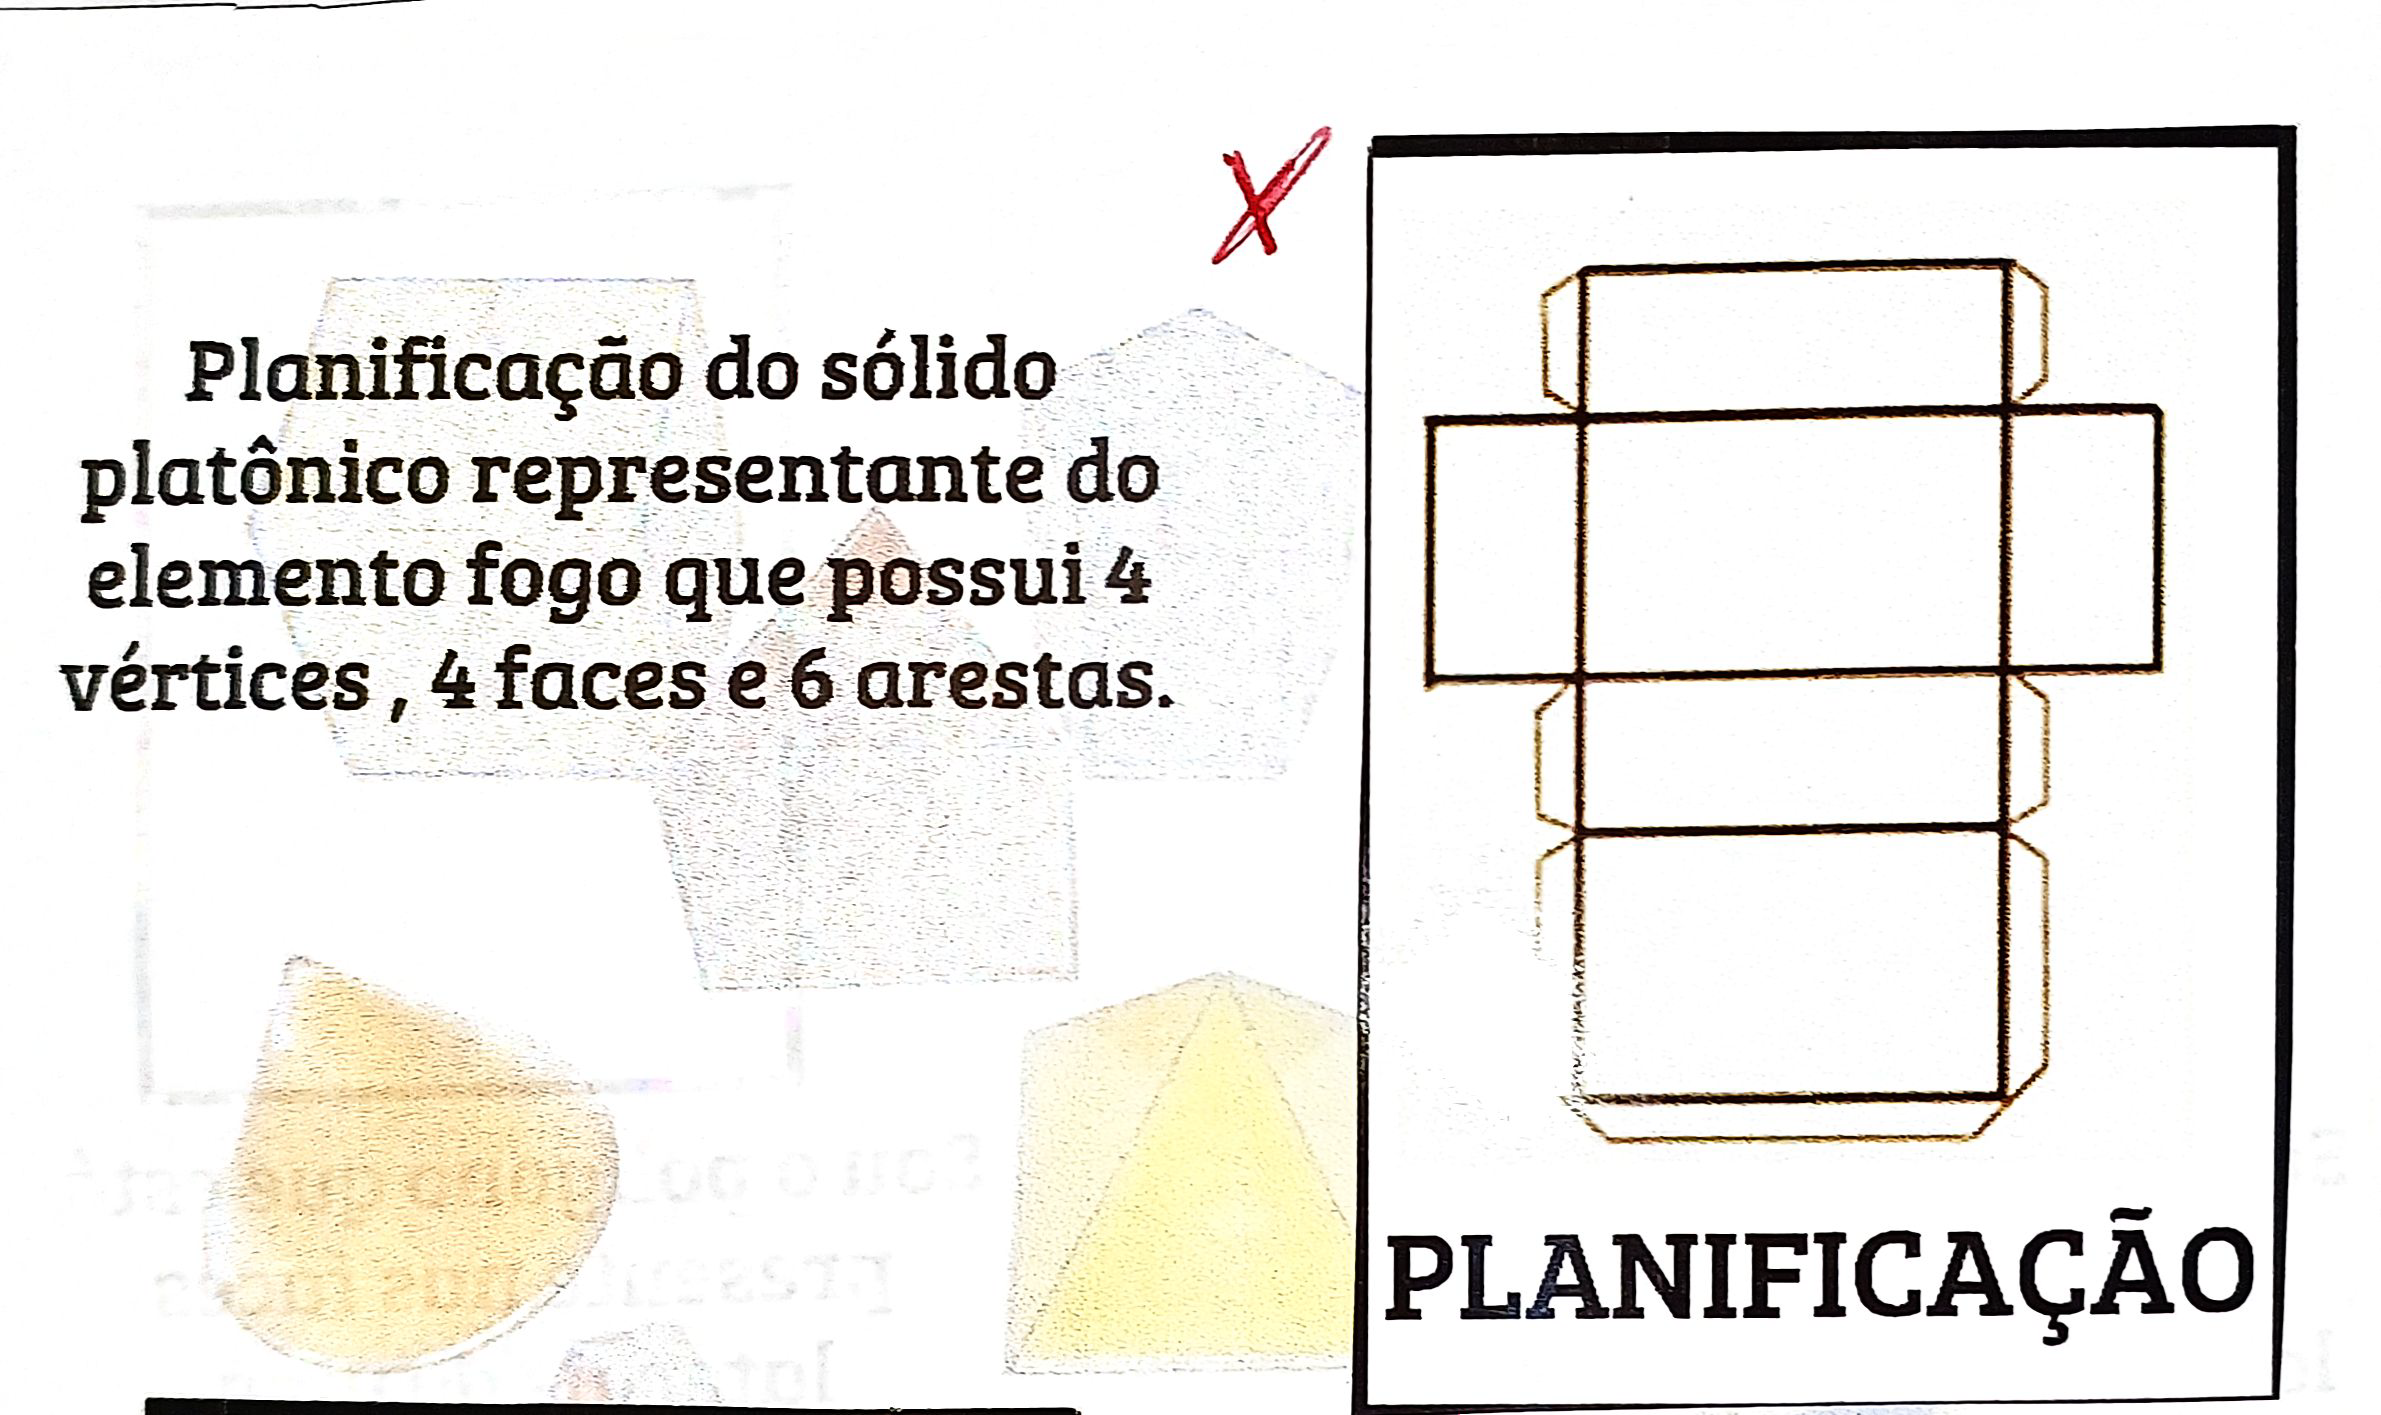
\includegraphics[width=0.5\textwidth]{Novas imagens/261 - Aulas 23 e 24 - Colagem incorreta no Álbum de Figurinhas}
    \legend{\autoria}
\end{CenteredFigure}

Notou-se que alguns alunos quando foram colar a última figura perceberam que colaram na posição errada (\autoref{fig: 259 - Aulas 23 e 24 - Colagem incorreta no Album de Figurinhas} e \autoref{fig: 261 - Aulas 23 e 24 - Colagem incorreta no Album de Figurinhas}) alguma figura pois a que sobrou não possuía as características descritas no espaço que sobrou no álbum. E aí, perguntaram se poderiam descolar. Os alunos conseguiram descolar e refazer, corretamente. Este fato possui vários significados e implicações educacionais a serem considerados:

\begin{enumerate}

    \item Autoconsciência e Autorreflexão:

          \begin{itemize}
              \item Desenvolvimento da Metacognição: O aluno está desenvolvendo a habilidade de pensar sobre seu próprio processo de aprendizado, identificando erros e compreendendo onde e por que cometeu esses erros.
              \item Autocrítica Construtiva: A capacidade de reconhecer os próprios erros é um passo importante para a autocrítica construtiva, que pode levar a uma melhoria contínua.
          \end{itemize}

    \item Independência e Autonomia:

          \begin{itemize}
              \item Resolução Independente de Problemas: A conclusão de que cometeu um erro sem a intervenção de um professor ou colega mostra que o aluno está adquirindo a capacidade de resolver problemas de forma independente.
              \item Autodisciplina: O aluno demonstra autodisciplina e responsabilidade pelo seu próprio aprendizado.
          \end{itemize}

    \item Motivação e Persistência:

          \begin{itemize}
              \item Motivação Intrínseca: A habilidade de reconhecer e corrigir erros por conta própria pode indicar uma alta motivação intrínseca, onde o aluno está genuinamente interessado em aprender e melhorar.
              \item Persistência: Concluir que errou e continuar tentando pode refletir a persistência do aluno diante de desafios.
          \end{itemize}

    \item Crescimento e Aprendizado:

          \begin{itemize}
              \item Oportunidade de Aprendizado: Reconhecer os erros é uma oportunidade para aprender com eles, ajustando estratégias e abordagens para evitar os mesmos erros no futuro.
              \item Crescimento Cognitivo: O processo de identificar e corrigir erros promove o crescimento cognitivo e o entendimento mais profundo dos conceitos.
          \end{itemize}

    \item Aspectos Psicológicos:

          \begin{itemize}
              \item Confiança e Autoestima: Dependendo da reação do aluno ao erro, isso pode impactar a confiança e autoestima. Um aluno que vê o erro como uma oportunidade para aprender pode desenvolver uma atitude positiva em relação à aprendizagem contínua.
          \end{itemize}

    \item Feedback e Melhorias:

          \begin{itemize}
              \item Feedback Interno: O aluno está desenvolvendo a habilidade de fornecer feedback interno, o que é crucial para a aprendizagem ao longo da vida.
              \item Ajuste de Estratégias: Reconhecer erros permite ao aluno ajustar suas estratégias de estudo e abordagem de problemas, melhorando assim seu desempenho futuro.
          \end{itemize}

\end{enumerate}

Em resumo, a capacidade de um aluno reconhecer sozinho que errou ao realizar uma atividade escolar é um sinal positivo de desenvolvimento de habilidades metacognitivas, independência, motivação intrínseca e potencial para crescimento acadêmico e pessoal.

\begin{table}[htbp] \centering
    \caption{Tabela de Acertos no Álbum de Figurinhas} \label{tab:Acertos do Encontro 12}
    \begin{tabular}{|c|c|}
        \hline
        \textbf{Aluno} & \textbf{Percentual de acertos} \\
        \hline
        1              & 100                            \\ \hline
        2              & 100                            \\ \hline
        3              & 90                             \\ \hline
        4              & 90                             \\ \hline
        5              & 100                            \\ \hline
        6              & 90                             \\ \hline
        7              & 100                            \\ \hline
        8              & 80                             \\ \hline
        9              & 70                             \\ \hline
        10             & 90                             \\ \hline
        11             & 60                             \\ \hline
        12             & 100                            \\ \hline
        13             & 100                            \\ \hline
        14             & 90                             \\ \hline
        15             & 100                            \\ \hline
        16             & 85                             \\ \hline
        17             & 100                            \\ \hline
        18             & 100                            \\ \hline
        19             & 85                             \\ \hline
        20             & 100                            \\ \hline
        21             & 50                             \\ \hline
        22             & 100                            \\ \hline
        23             & 80                             \\ \hline
    \end{tabular}
    \legend{\legendaTabela}
\end{table}

Portanto, como mostra a \autoref{tab:Acertos do Encontro 12}, observou-se que:

\begin{itemize}
    \item 48\% da turma teve 100\% de acerto
    \item 22\% da turma teve 90\% de acerto
    \item 9\% da turma teve 85\% de acerto
    \item 9\% da turma teve 80\% de acerto
    \item 4\% da turma teve 70\% de acerto
    \item 4\% da turma teve 60\% de acerto
    \item 4\% da turma teve 50\% de acerto
\end{itemize}

A tabulação do percentual de acertos das atividades de todos os encontros foi feita na planilha Excel. O resultado percentual médio, por aluno, ao final deste projeto é apresentado pela \autoref{tab:Resultado Final do Projeto}.

\begin{table}[htbp] \centering
    \caption{Média percentual de Acertos nas 12 atividades deste projeto} \label{tab:Resultado Final do Projeto}
    \begin{tabular}{|c|c|}
        \hline
        \textbf{Aluno} & \textbf{Percentual de acertos} \\
        \hline
        1              & 89                             \\ \hline
        2              & 87                             \\ \hline
        3              & 79                             \\ \hline
        4              & 54                             \\ \hline
        5              & 78                             \\ \hline
        6              & 68                             \\ \hline
        7              & 88                             \\ \hline
        8              & 64                             \\ \hline
        9              & 85                             \\ \hline
        10             & 73                             \\ \hline
        11             & 59                             \\ \hline
        12             & 88                             \\ \hline
        13             & 75                             \\ \hline
        14             & 36                             \\ \hline
        15             & 33                             \\ \hline
        16             & 56                             \\ \hline
        17             & 54                             \\ \hline
        18             & 57                             \\ \hline
        19             & 73                             \\ \hline
        20             & 87                             \\ \hline
        21             & 58                             \\ \hline
        22             & 75                             \\ \hline
        23             & 55                             \\ \hline
    \end{tabular}
    \legend{\legendaTabela}
\end{table}
\newpage

\section{Avaliação da sequência de atividades pelos pelos alunos}

A abordagem incentiva a participação ativa dos alunos, uma vez que eles precisam discutir, argumentar e justificar suas ideias. Isso pode aumentar o interesse e o engajamento nas aulas. Ao explorar problemas relacionados ao mundo real, os alunos conseguem ver a aplicação prática dos conceitos geométricos, o que pode tornar o aprendizado mais significativo.

Trabalhar em grupo para resolver problemas pode ajudar aos alunos a desenvolver habilidades de comunicação e colaboração, importantes tanto para a vida acadêmica quanto para a vida profissional. Os alunos são incentivados a pensar de forma criativa e a aplicar conhecimentos teóricos para resolver problemas práticos, o que fortalece sua capacidade de resolver problemas em contextos variados.

Alguns problemas podem ser complexos e desafiadores, o que pode ser frustrante para alunos com dificuldades ou pouco interesse em matemática. Para que a metodologia fosse eficaz, foi necessário um planejamento cuidadoso por parte do professor para garantir que os problemas fossem apropriados ao nível dos estudantes e que todas as fases do processo de resolução fossem adequadamente guiadas.

Avaliar esse processo de Resolução de Problemas foi desafiador, pois envolveu não apenas a solução final, mas o processo de pensamento e as estratégias utilizadas pelos estudantes.

A Metodologia de Resolução de Problemas é uma ferramenta poderosa no ensino de Geometria Espacial e poliedros, promovendo um aprendizado mais ativo e significativo. No entanto, seu sucesso depende de uma implementação cuidadosa e do suporte contínuo aos estudantes durante o processo.

Baseado nos resultados da avaliação realizada com os estudantes, constatou-se que a sequência de atividades são excelentes ferramentas pedagógicas, visto que trabalham os conteúdos de maneira divertida e prazerosa, despertando a curiosidade dos alunos, auxiliando na aprendizagem.

Essa abordagem destaca a importância de diversificar as atividades pedagógicas para despertar o interesse dos alunos e melhorar a eficácia do ensino-aprendizagem. A utilização de diferentes ferramentas, é considerada uma aliada poderosa para os professores atingirem seus objetivos pedagógicos. As sequências de atividades, em particular, são vistas como uma estratégia eficaz para engajar os alunos e facilitar a aprendizagem. A expectativa é que os resultados desta pesquisa inspirem professores de diversas áreas do conhecimento a integrarem mais atividades diversificadas com a metodologia baseada em problemas em suas práticas pedagógicas, reconhecendo seu valor na formação integral dos estudantes.

Por meio da sequência de atividades, os estudantes aprenderam muito além da simples prática de copiar os conteúdos e realizar listas de exercício sobre ele, pois promovem a socialização entre alunos e professor, assim como a cooperação, sendo um recurso importante para abordar diversas temáticas que percorrem o currículo. As atividades utilizando a metodologia baseada em problemas, não trazem respostas prontas, mas favorecem a investigação, a pesquisa e a reflexão envolta de situações problema.

\begin{CenteredFigure}
    \caption{Satisfação dos alunos por aula - Parte 1} \label{fig:satisfacao1}
    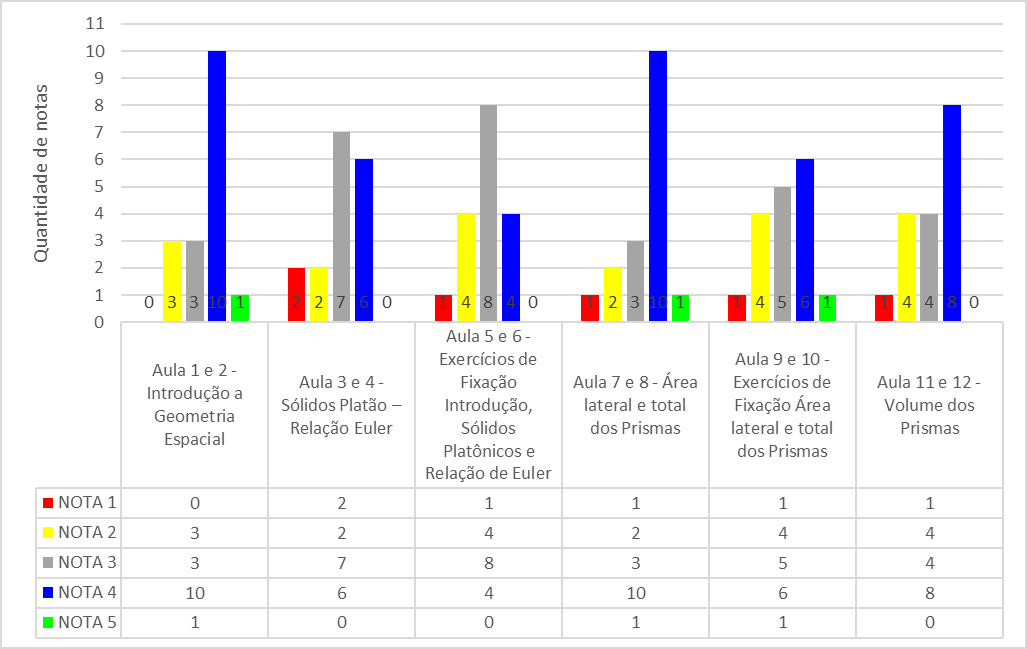
\includegraphics[width=\linewidth]{Satisfação dos alunos por aula - 1}
    \legend{\autoria}
\end{CenteredFigure}

\begin{CenteredFigure}
    \caption{Satisfação dos alunos por aula - Parte 2} \label{fig:satisfacao2}
    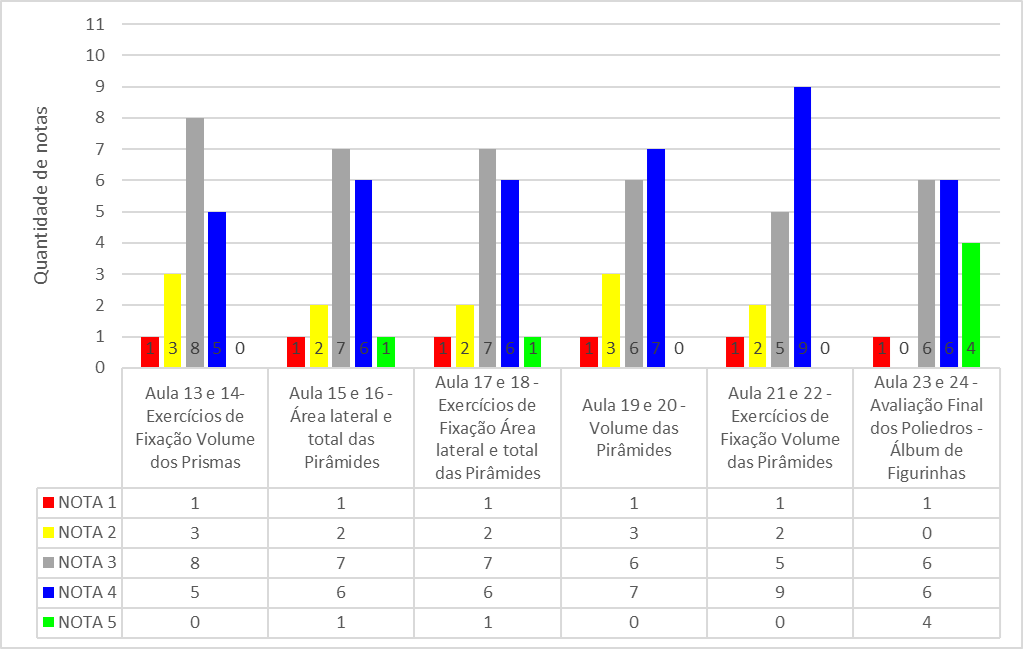
\includegraphics[width=\linewidth]{Satisfação dos alunos por aula - 2}
    \legend{\autoria}
\end{CenteredFigure}

A análise dos gráficos de notas atribuídas pelos alunos às aulas de Geometria Espacial (\autoref{fig:satisfacao1} e \autoref{fig:satisfacao2}) revela uma tendência geral de satisfação positiva. A maioria das aulas recebeu predominantemente Notas 3 e 4, indicando que os alunos consideraram as aulas boas, com algumas variando entre satisfatórias e muito boas. Aulas como ``Introdução a Geometria Espacial'' e ``Exercícios de Fixação: Área lateral e total dos Prismas'' destacaram-se com Notas 4, mostrando uma aceitação particularmente boa. Em contraste, poucas aulas receberam Notas 5, sugerindo que, embora bem recebidas, poucas foram consideradas excelentes. Notas 1 e 2 apareceram em menor quantidade, indicando que a insatisfação foi relativamente baixa. Essa distribuição aponta para uma experiência de aprendizado positiva, com algumas áreas de melhorias para alcançar níveis de excelência percebidos pelos alunos.

\chapter{Considerações Finais} \label{cap:5_consideracoes}

Nesta pesquisa, preocupou-se em estimular o aluno a pensar e a participar ativamente da construção de novos conhecimentos. Assim, ao trabalhar com a Metodologia de Ensino-Aprendizagem-Avaliação de Matemática através da Resolução de Problemas, ficou evidente que, provocou-se os alunos para que, ao buscar a resolução, pensassem, refletissem e, com segurança, a encontrassem.

Portanto, agora que se finalizou a pesquisa, pode-se responder à pergunta lançada no início da mesma: O uso da Metodologia de Ensino-Aprendizagem-Avaliação de Matemática através da Resolução de Problemas constitui-se num caminho alternativo para a construção de conceitos e conteúdos geométricos espaciais pelos alunos do Ensino Médio?

Consegue-se demonstrar que a Resolução de Problemas é um dos principais métodos para ensinar, aprender e avaliar a Matemática em sala de aula. Conforme afirmou \citeonline[p. 40]{van_de_walle_elementary_2000}, a maioria, senão todos, os conceitos e procedimentos matemáticos importantes podem ser melhor ensinados através da Resolução de Problemas. Ou seja, tarefas ou problemas podem e devem ser propostos de modo a engajar os estudantes no pensar e promover um aprendizado mais profundo e significativo.

Com base nas evidências coletadas nesta pesquisa, acredita-se fortemente que a Metodologia de Ensino-Aprendizagem-Avaliação de Matemática através da Resolução de Problemas é uma alternativa eficaz que permite aos alunos a construção de conceitos e conteúdos matemáticos, explorando e aproveitando seu próprio potencial e habilidades. Os alunos ficaram comprometidos com o trabalho e focados nas atividades propostas, não havendo dispersão. Conseguiu-se também, uma evolução significativa dos rendimentos qualitativos e quantitativos. A Resolução de Problemas se torna, assim, um recurso valioso não só para ensinar, mas também para aprender e praticar Matemática. Por fim, espera-se que a pesquisa suscite novos questionamentos e que ajude aos professores a reconhecerem o valor da Matemática na formação de cidadãos críticos e reflexivos, essenciais para uma sociedade em constante mudança.

\section{Trabalhos futuros}

Para futuros trabalhos, várias direções promissoras podem ser exploradas, visando aprofundar e ampliar os resultados obtidos. Primeiramente, seria interessante investigar a aplicação da Metodologia de Ensino-Aprendizagem-Avaliação de Matemática através da Resolução de Problemas em diferentes contextos educacionais, incluindo escolas públicas e privadas, e em diversas regiões geográficas, para verificar a generalidade dos resultados.

Outro caminho a ser explorado é a aplicação dessa metodologia em outras áreas da matemática além da geometria espacial, como álgebra, estatística e cálculo, para avaliar sua eficácia em diferentes conteúdos e níveis de complexidade. Além disso, seria valioso conduzir estudos longitudinais para acompanhar o desenvolvimento dos alunos ao longo do tempo, verificando o impacto a longo prazo da Resolução de Problemas em suas habilidades matemáticas e em seu desempenho acadêmico geral.

Também seria enriquecedor desenvolver e testar novas ferramentas e recursos didáticos que possam complementar a metodologia de Resolução de Problemas, como o uso de tecnologias educacionais, jogos matemáticos e atividades colaborativas, e avaliar como esses recursos podem potencializar a aprendizagem e o engajamento dos alunos.

Adicionalmente, a formação e o desenvolvimento profissional dos professores que utilizam essa metodologia merecem atenção especial. Investigar as melhores práticas para capacitar e apoiar os professores na implementação eficaz da Resolução de Problemas em suas salas de aula pode contribuir significativamente para a disseminação e o sucesso da metodologia.

Por fim, uma abordagem interessante seria a análise comparativa entre a Metodologia de Ensino-Aprendizagem-Avaliação de Matemática através da Resolução de Problemas e outras metodologias inovadoras de ensino, como a aprendizagem baseada em projetos ou a sala de aula invertida. Isso permitiria identificar pontos fortes e áreas de melhoria, além de possibilitar a combinação de diferentes estratégias para um ensino de matemática ainda mais eficaz.

Em resumo, futuras pesquisas podem expandir o conhecimento sobre a metodologia de Resolução de Problemas, explorando sua aplicação em diferentes contextos e conteúdos, desenvolvendo novos recursos didáticos, focando na formação de professores e comparando-a com outras abordagens inovadoras. Esperamos que esses trabalhos futuros contribuam para a evolução contínua do ensino de matemática, promovendo uma educação mais dinâmica, envolvente e significativa para os alunos.

%\chapter{Considerações Finais}

% --- ELEMENTOS PÓS-TEXTUAIS ---

\postextual

% ----------------------------------------------------------
% Referências bibliográficas
% ----------------------------------------------------------
\bibliography{Fernanda}

% --- Apêndices ---

% --- Inicia os apêndices ---
\begin{apendicesenv}

    \partapendices % Imprime uma página indicando o início dos apêndices

    % ----------------------------------------------------------
    \chapter{Autorização da Direção e Termo de Compromisso} \label{ApendiceA}

    % \chapter{Autorização da Direção}
    \label{ApendiceA.1}
    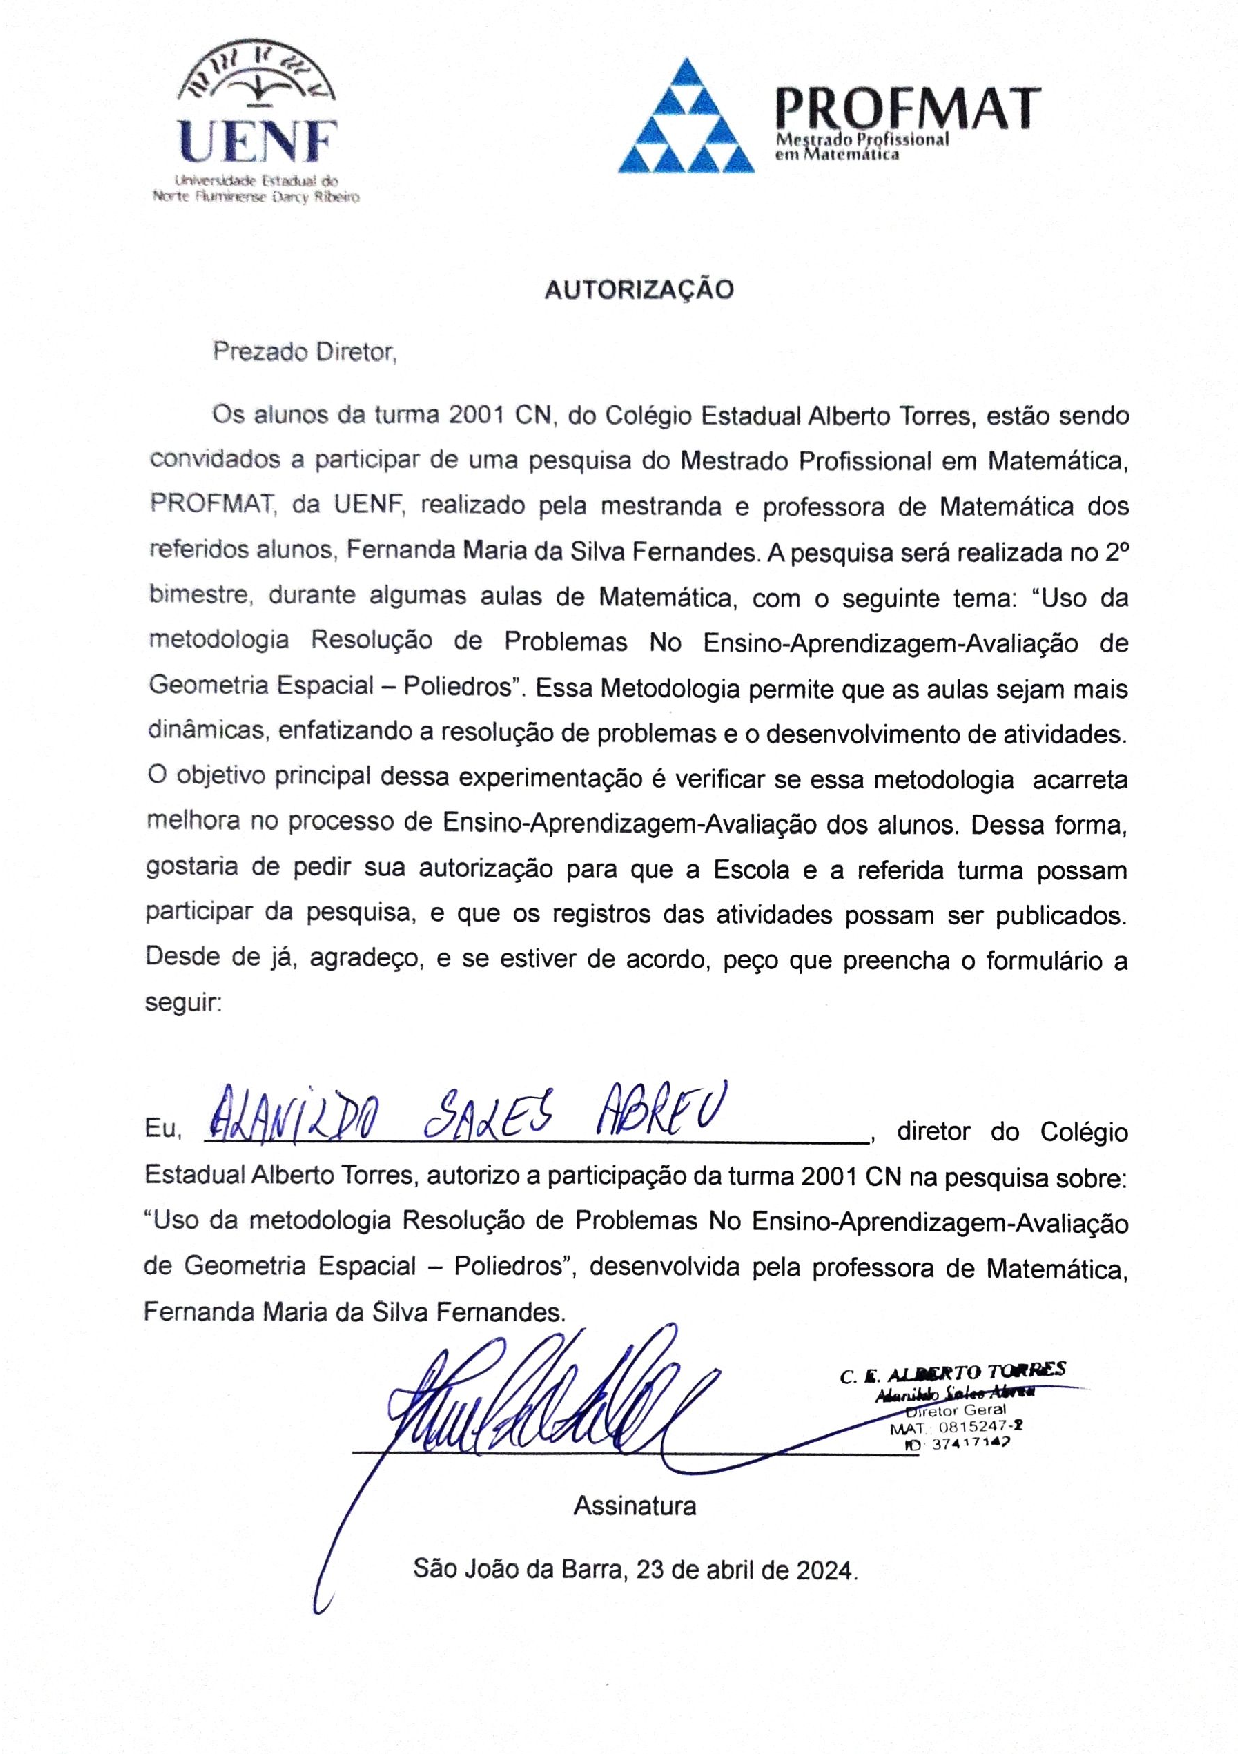
\includepdf[pages=-]{PDFs/AutorizacaoDiretor.pdf}

    % \chapter{Termo de Compromisso}
    \label{ApendiceA.2}
    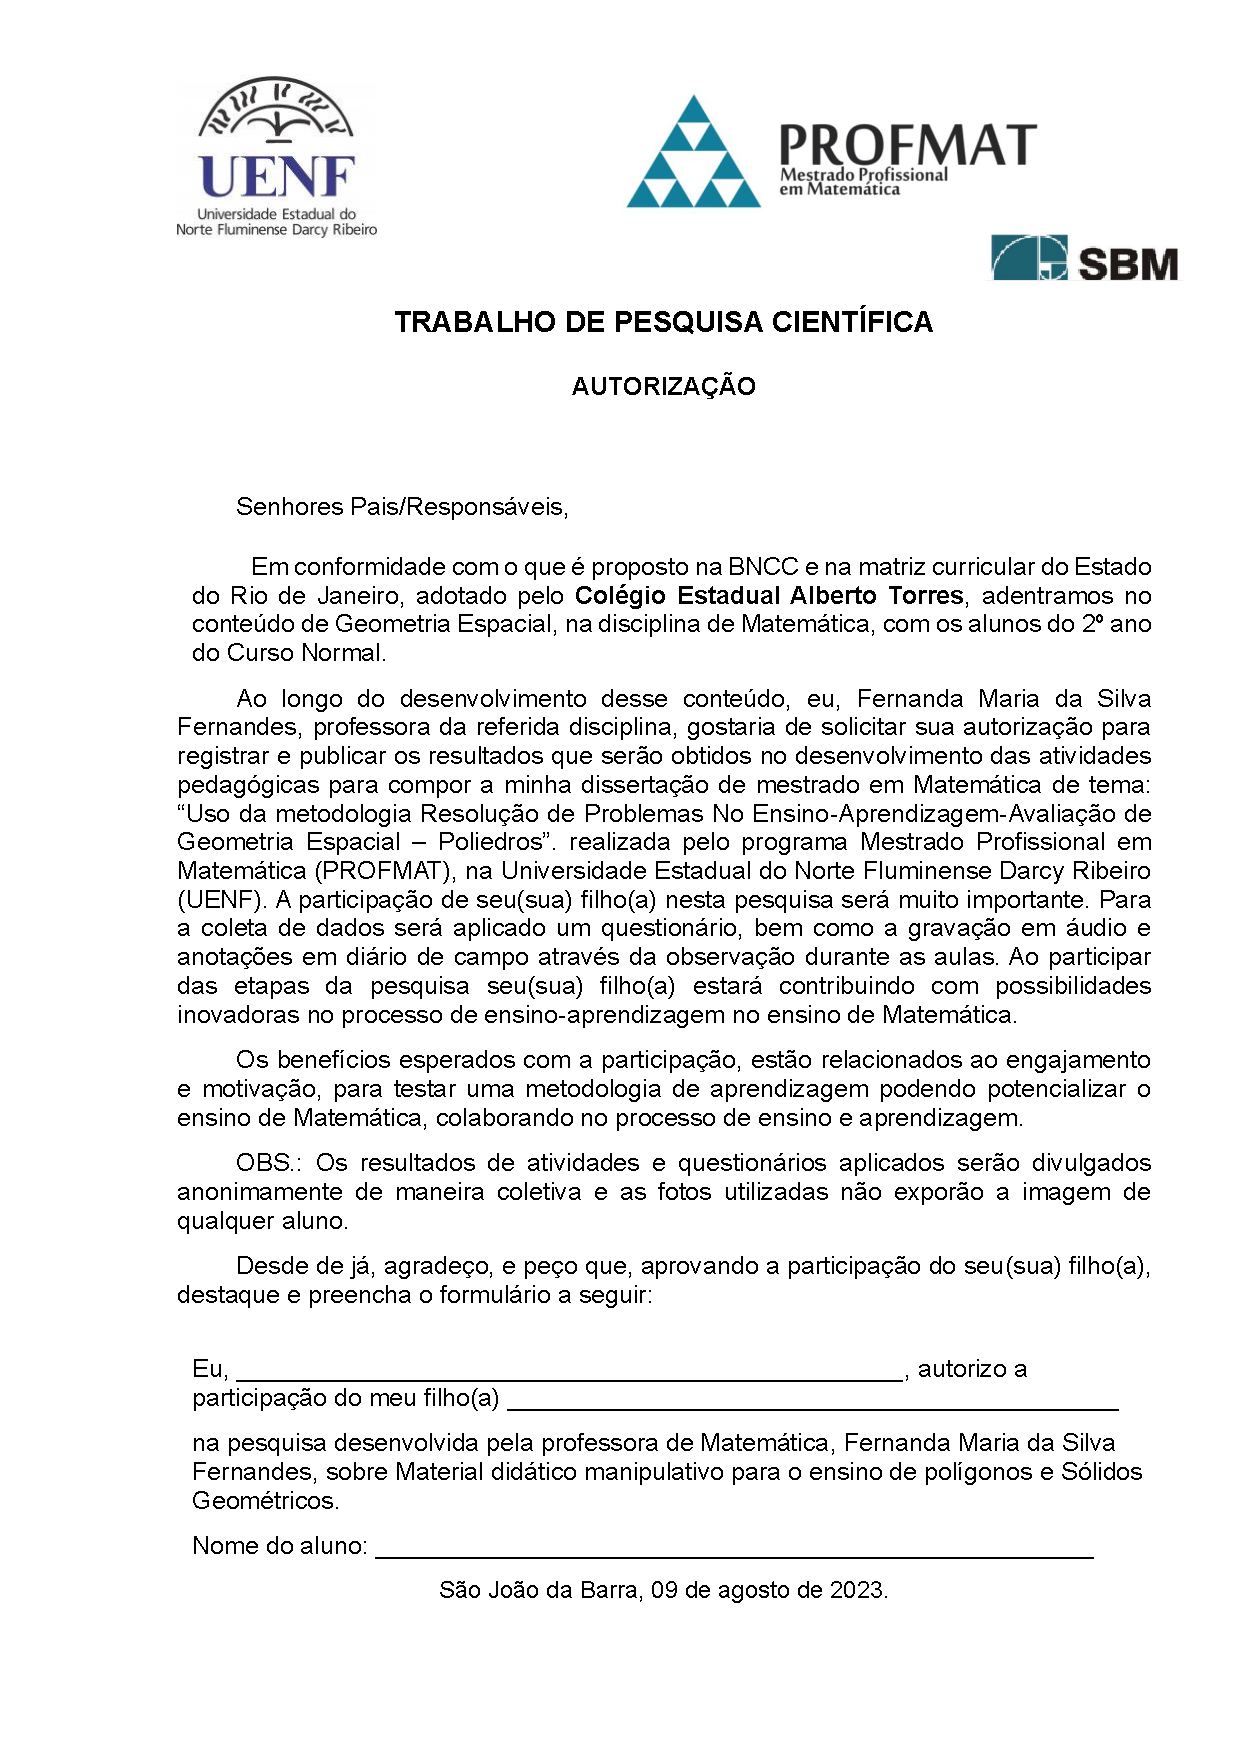
\includepdf[pages=-]{PDFs/AutorizacaoPaisResponsaveis.pdf}
    % ----------------------------------------------------------

    \chapter{Encontros}
    % \chapter{Aulas 1 e 2}
    \label{ApendiceB}
    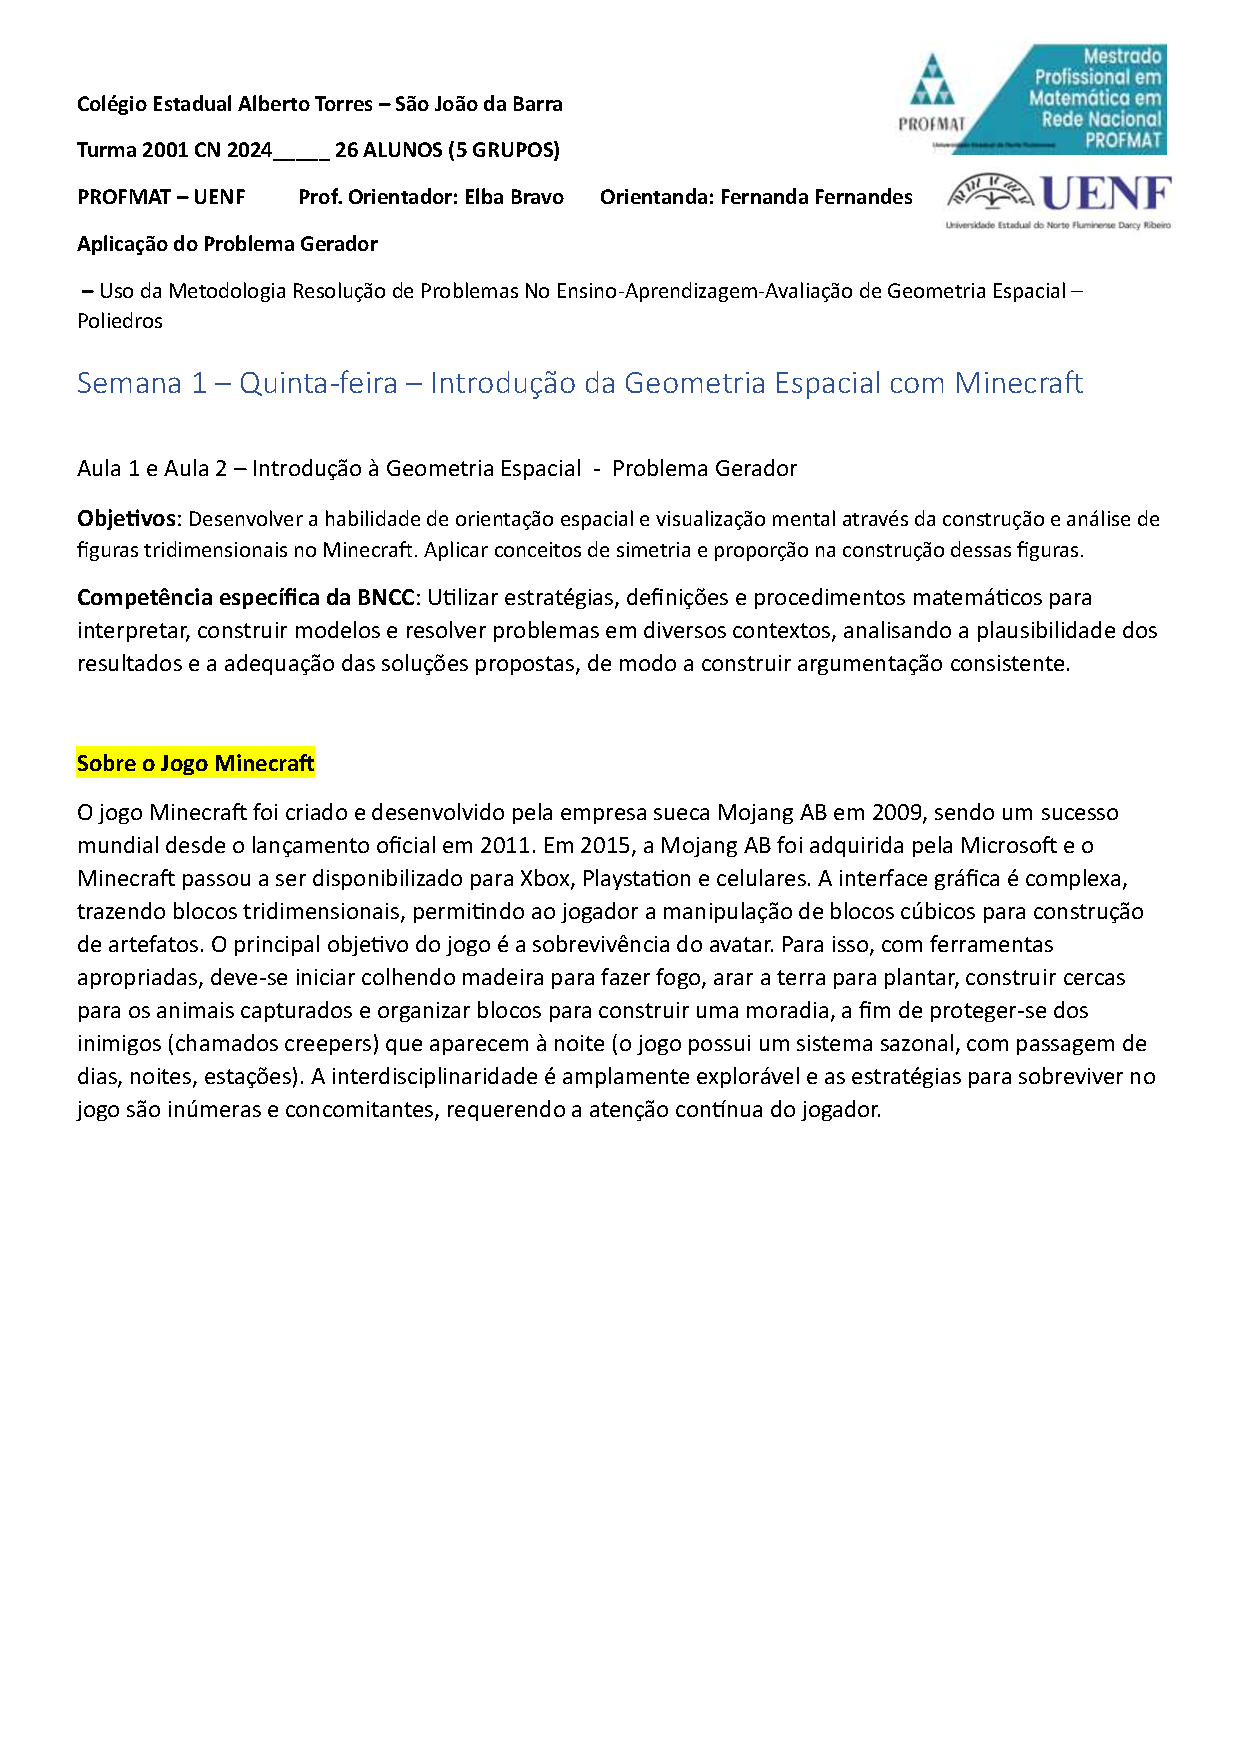
\includepdf[pages={1-3}]{Aulas/pdf1e2}

    % \chapter{Aulas 3 e 4}
    % \label{ApendiceC}
    % 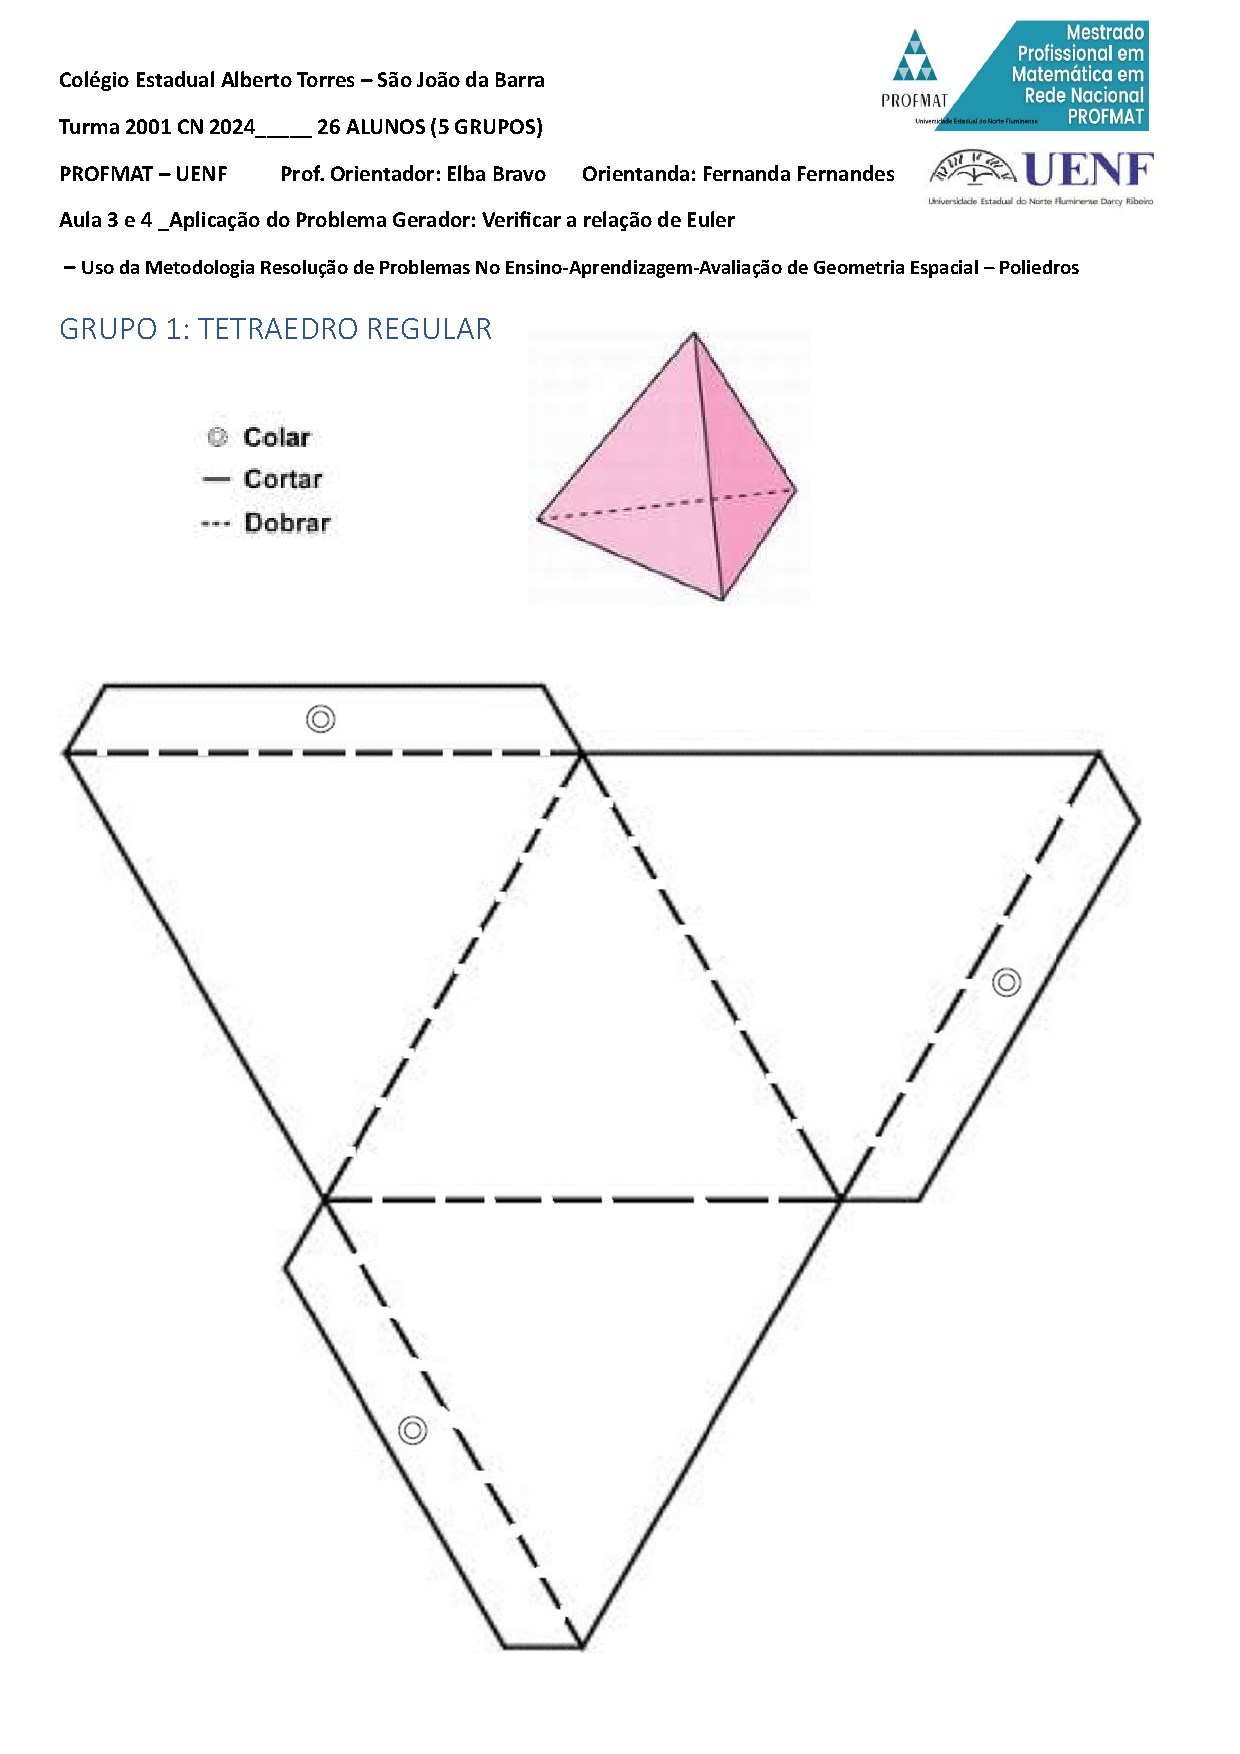
\includepdf[pages=-]{Aulas/pdf3e4}

    % \chapter{Aulas 3 e 4}
    \label{ApendiceC}
    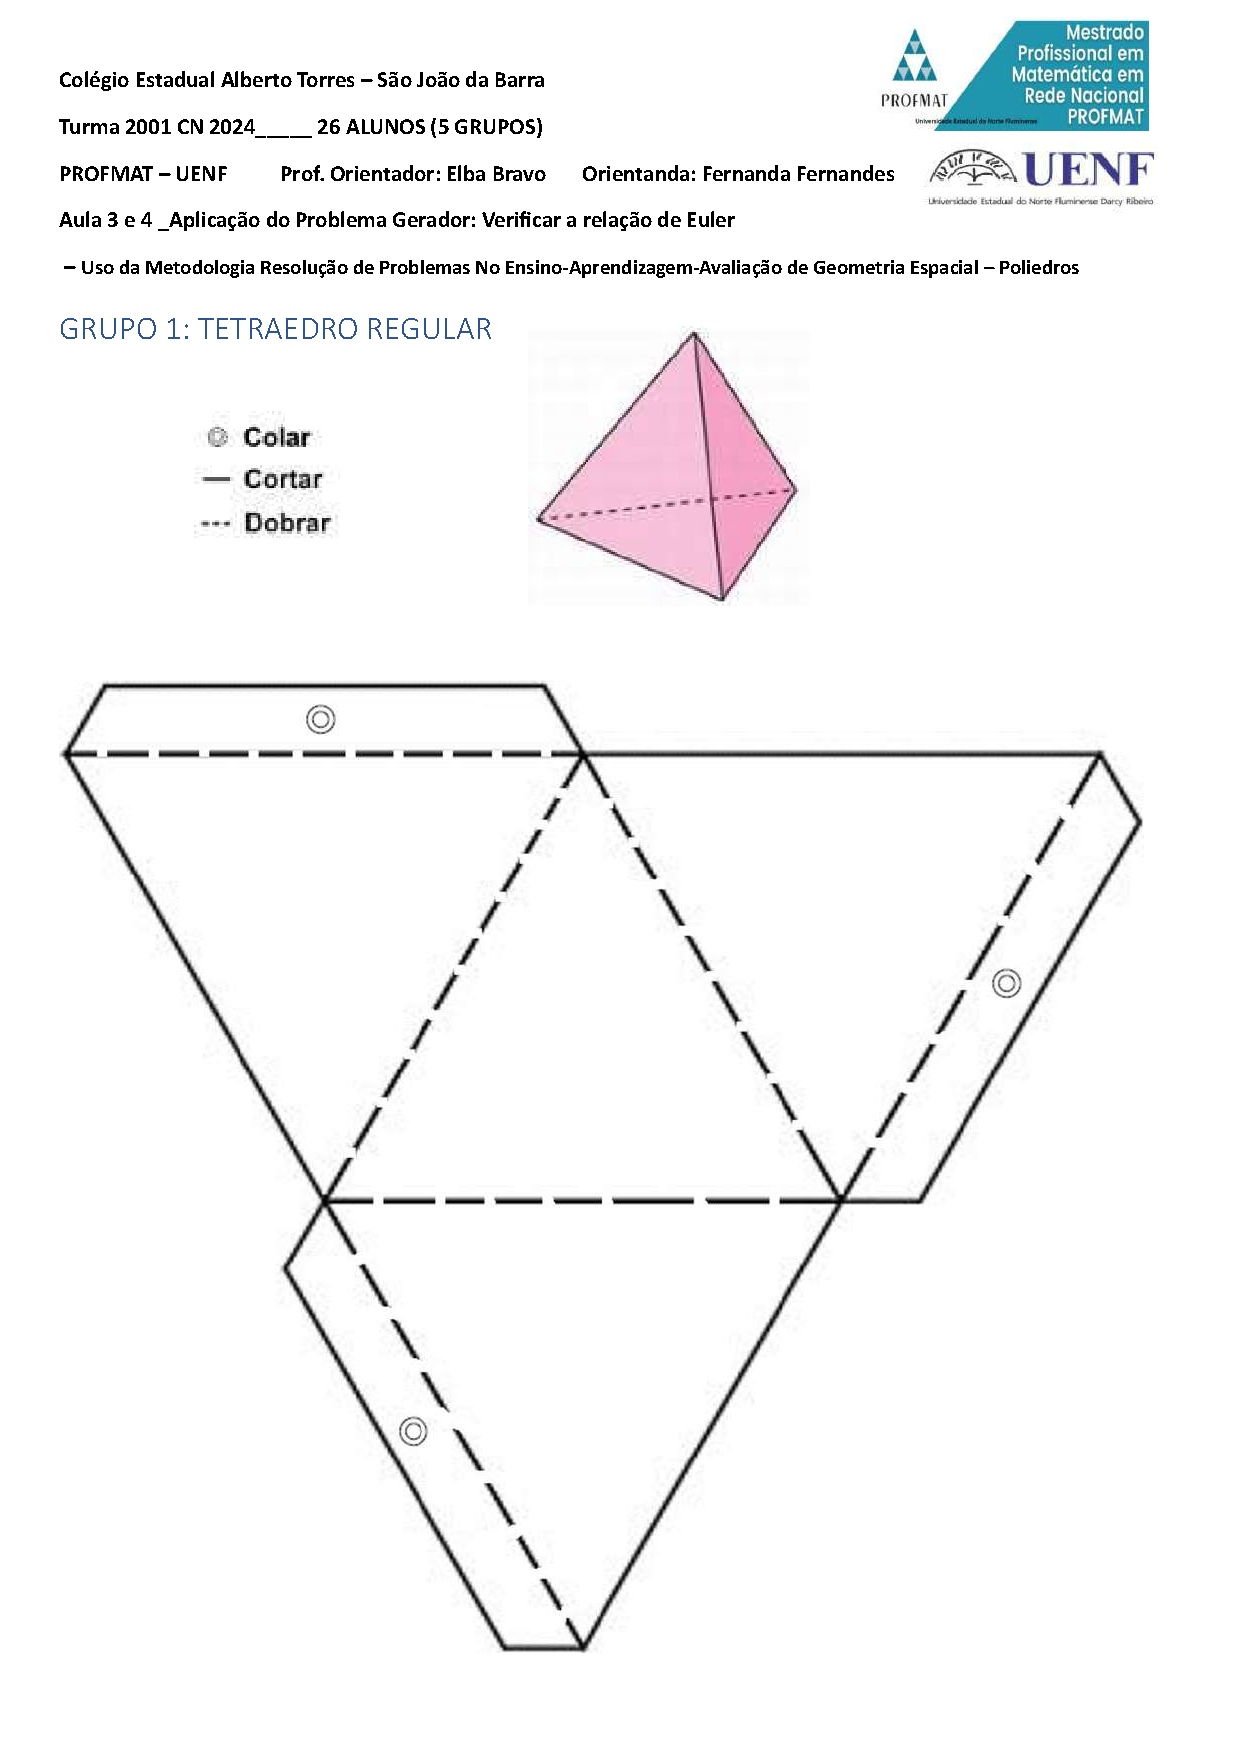
\includepdf[pages=-]{Aulas/pdf3e4_compressed}

    % \chapter{Aulas 5 e 6}
    \label{ApendiceD}
    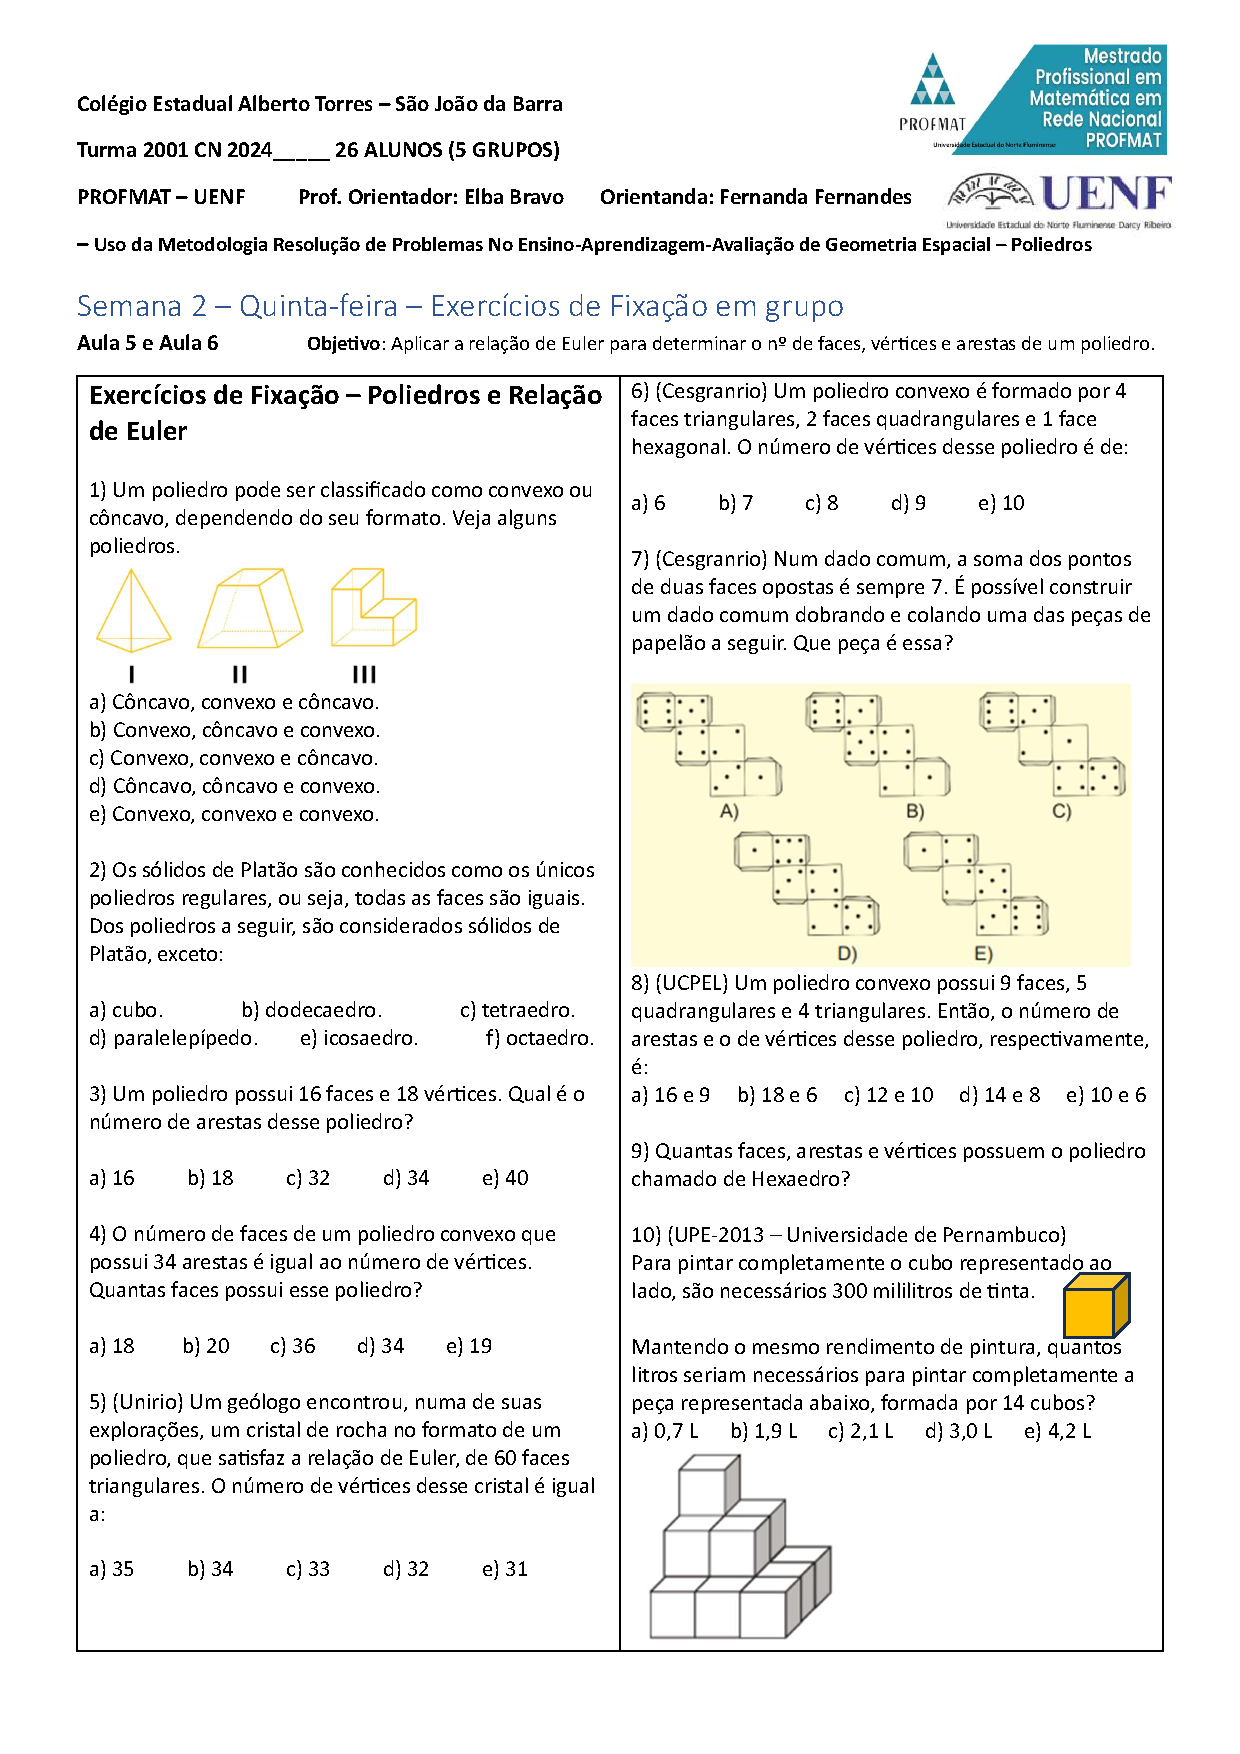
\includepdf[pages={1-3}]{Aulas/pdf5e6}

    % \chapter{Aulas 7 e 8}
    % \label{ApendiceE}
    % 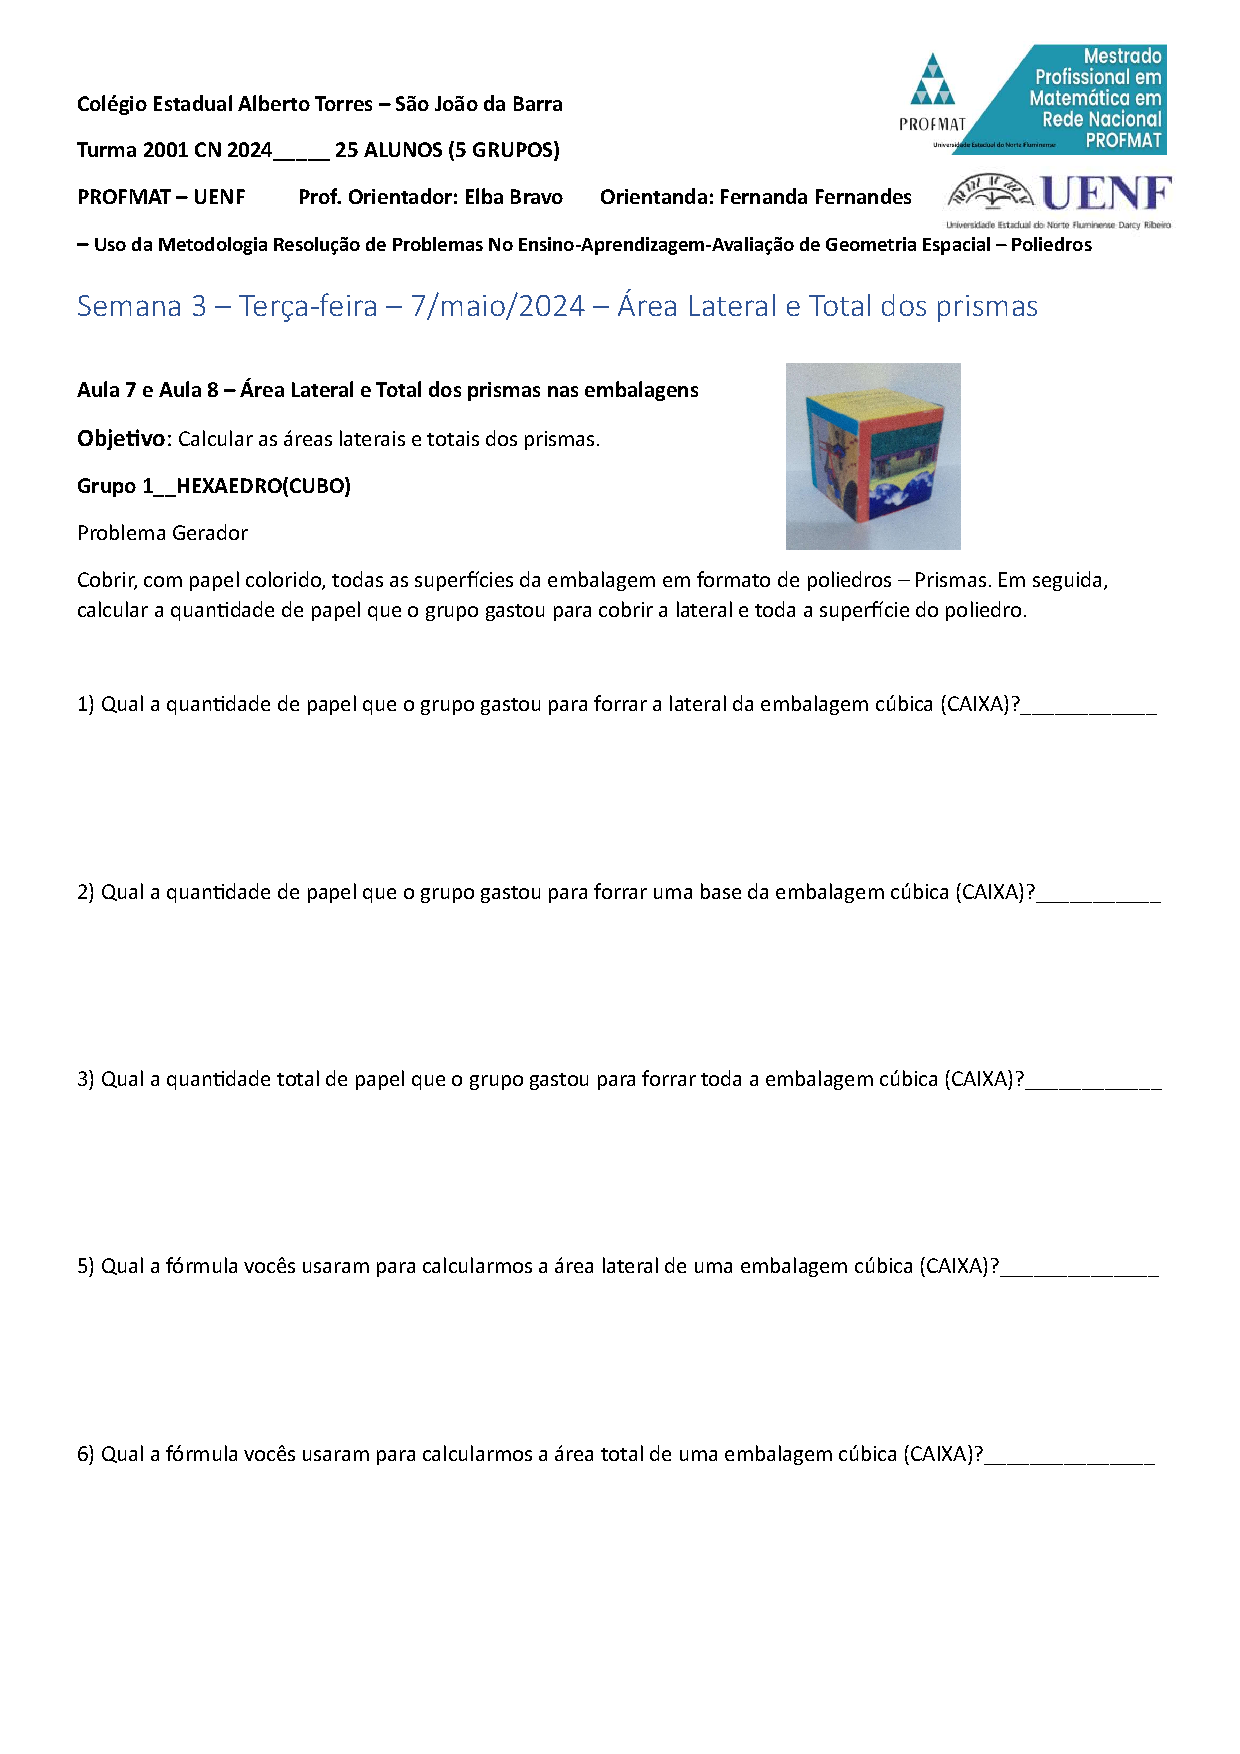
\includepdf[pages=-]{Aulas/pdf7e8}

    % \chapter{Aulas 7 e 8}
    \label{ApendiceE}
    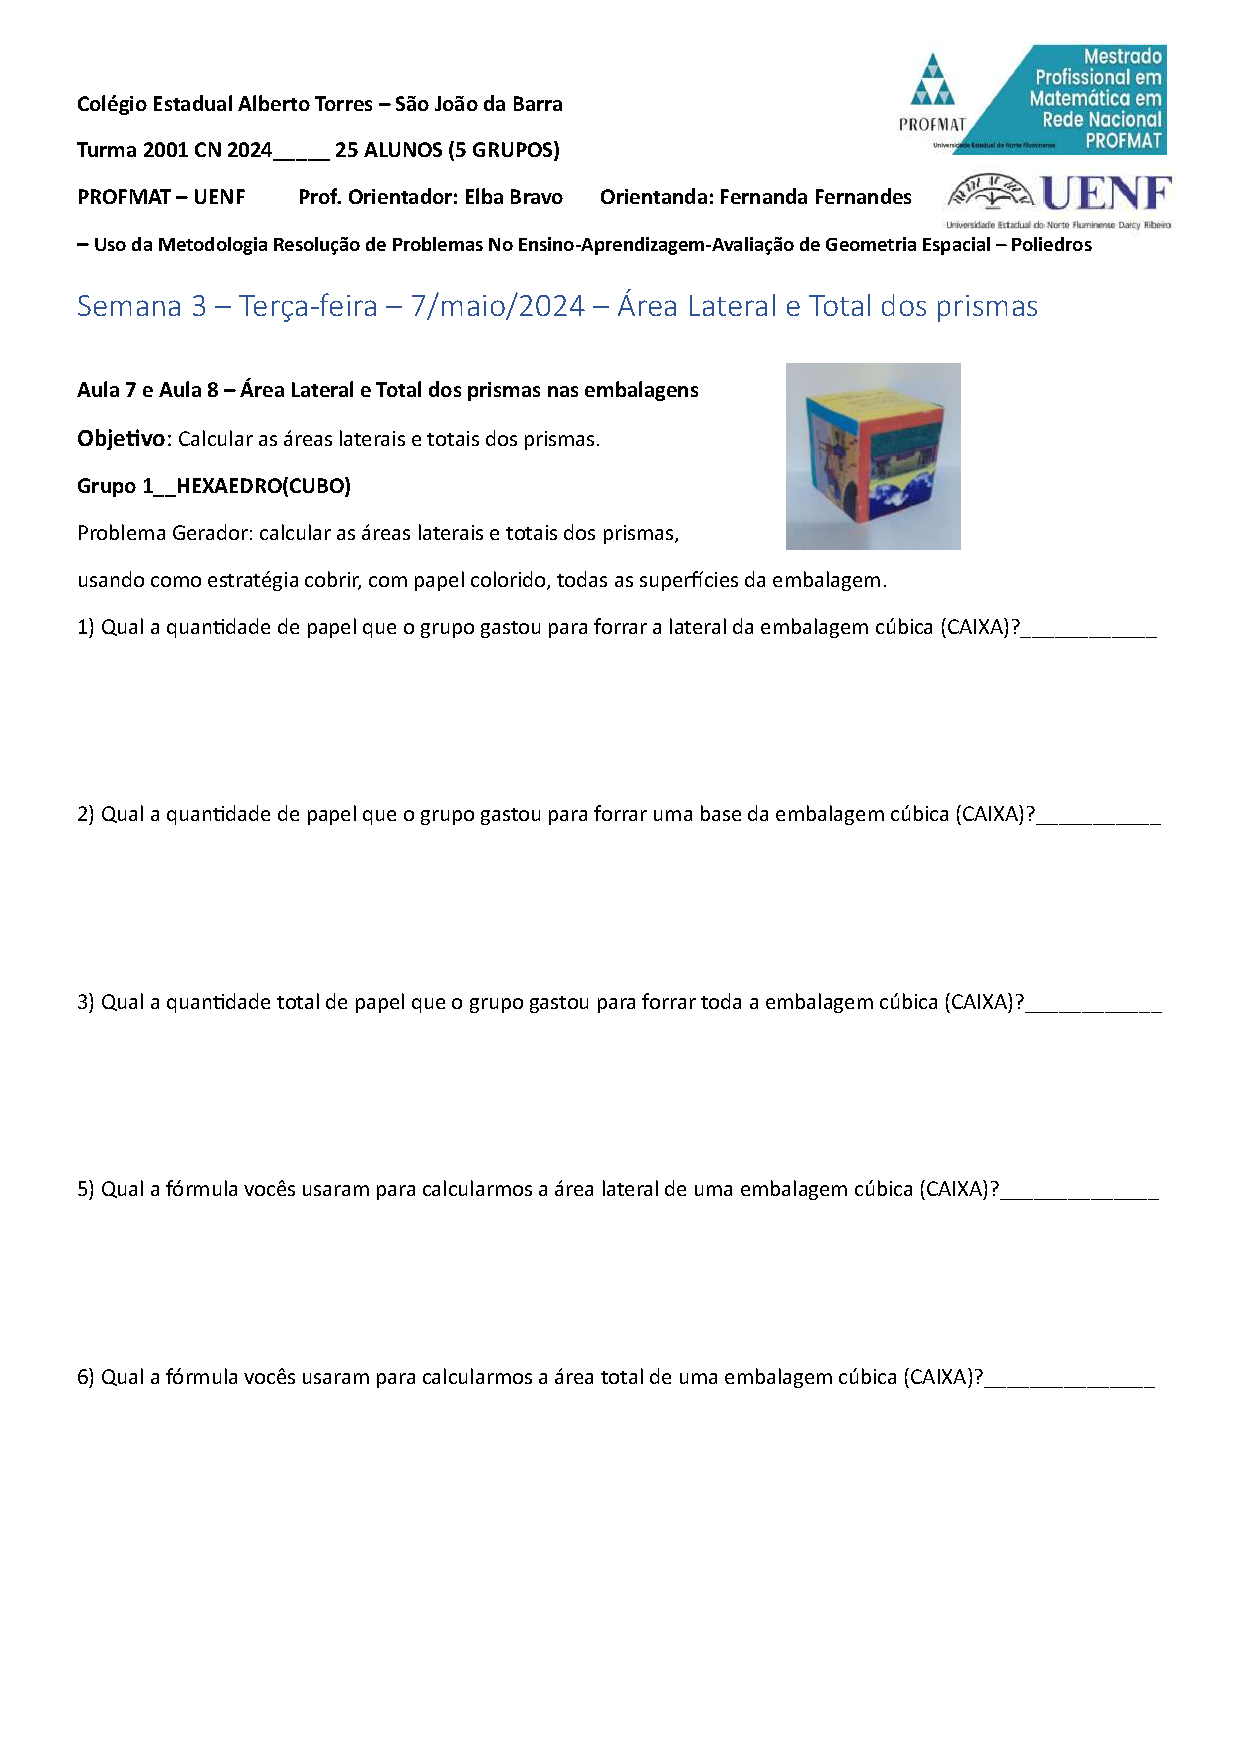
\includepdf[pages=-]{Aulas/pdf7e8_compressed}

    % \chapter{Aulas 9 e 10}
    \label{ApendiceF}
    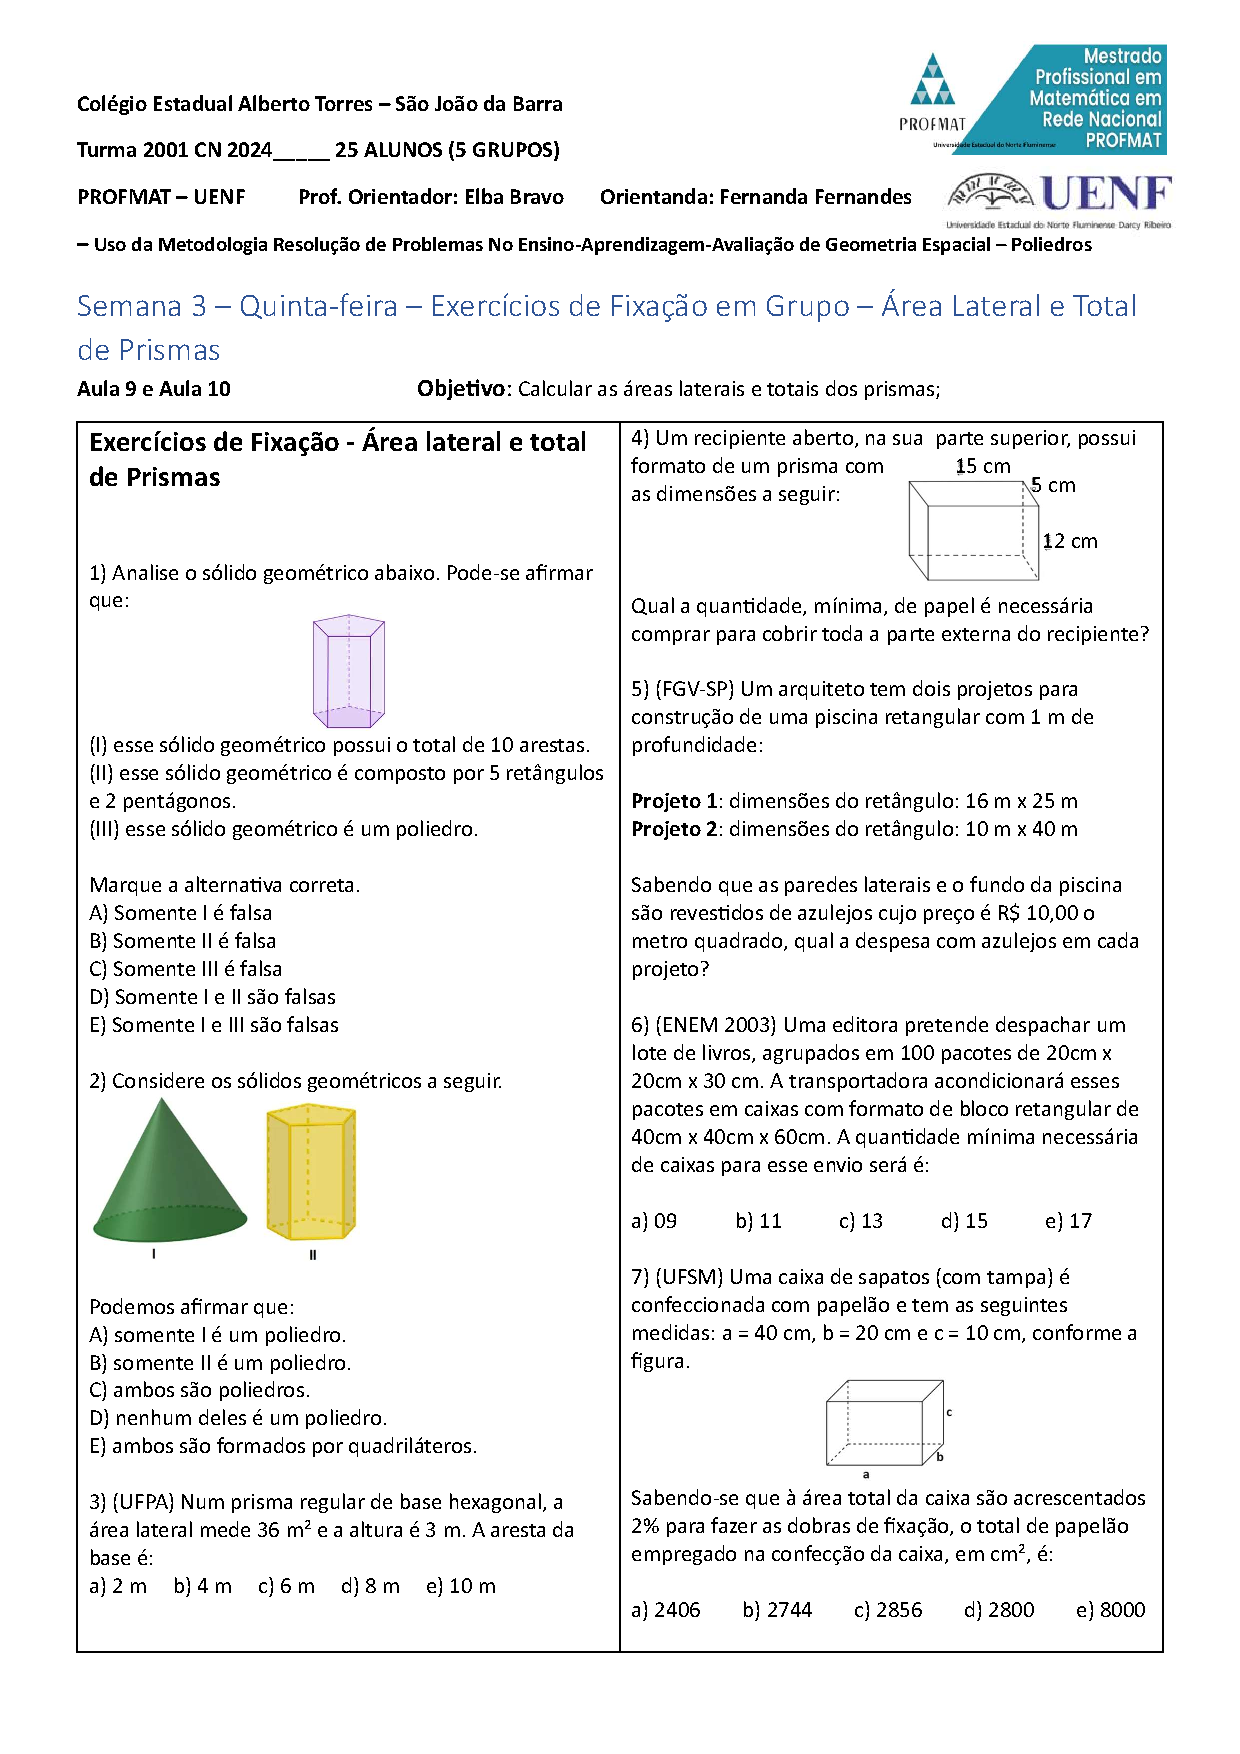
\includepdf[pages=-]{Aulas/pdf9e10}

    % \chapter{Aulas 11 e 12}
    % \label{ApendiceG}
    % 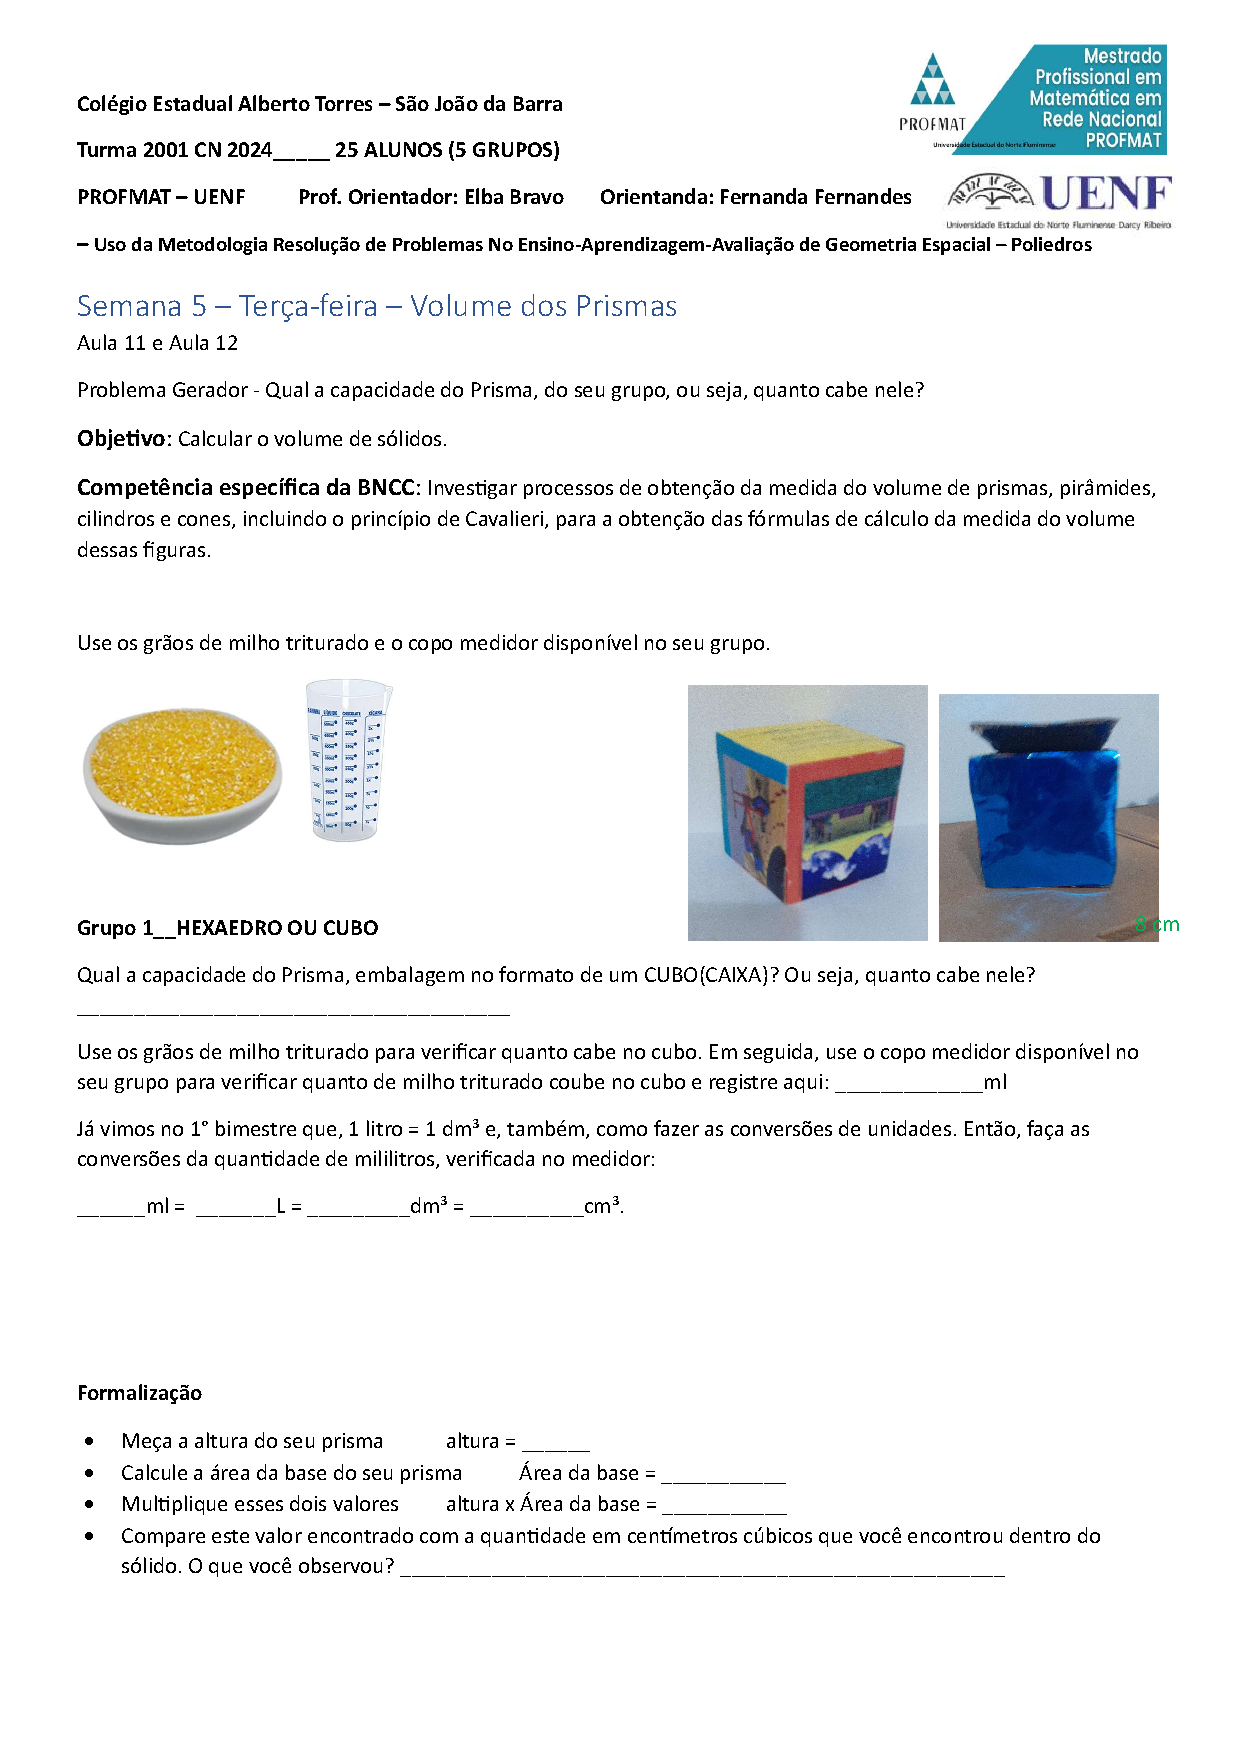
\includepdf[pages=-]{Aulas/pdf11e12}

    % \chapter{Aulas 11 e 12}
    \label{ApendiceG}
    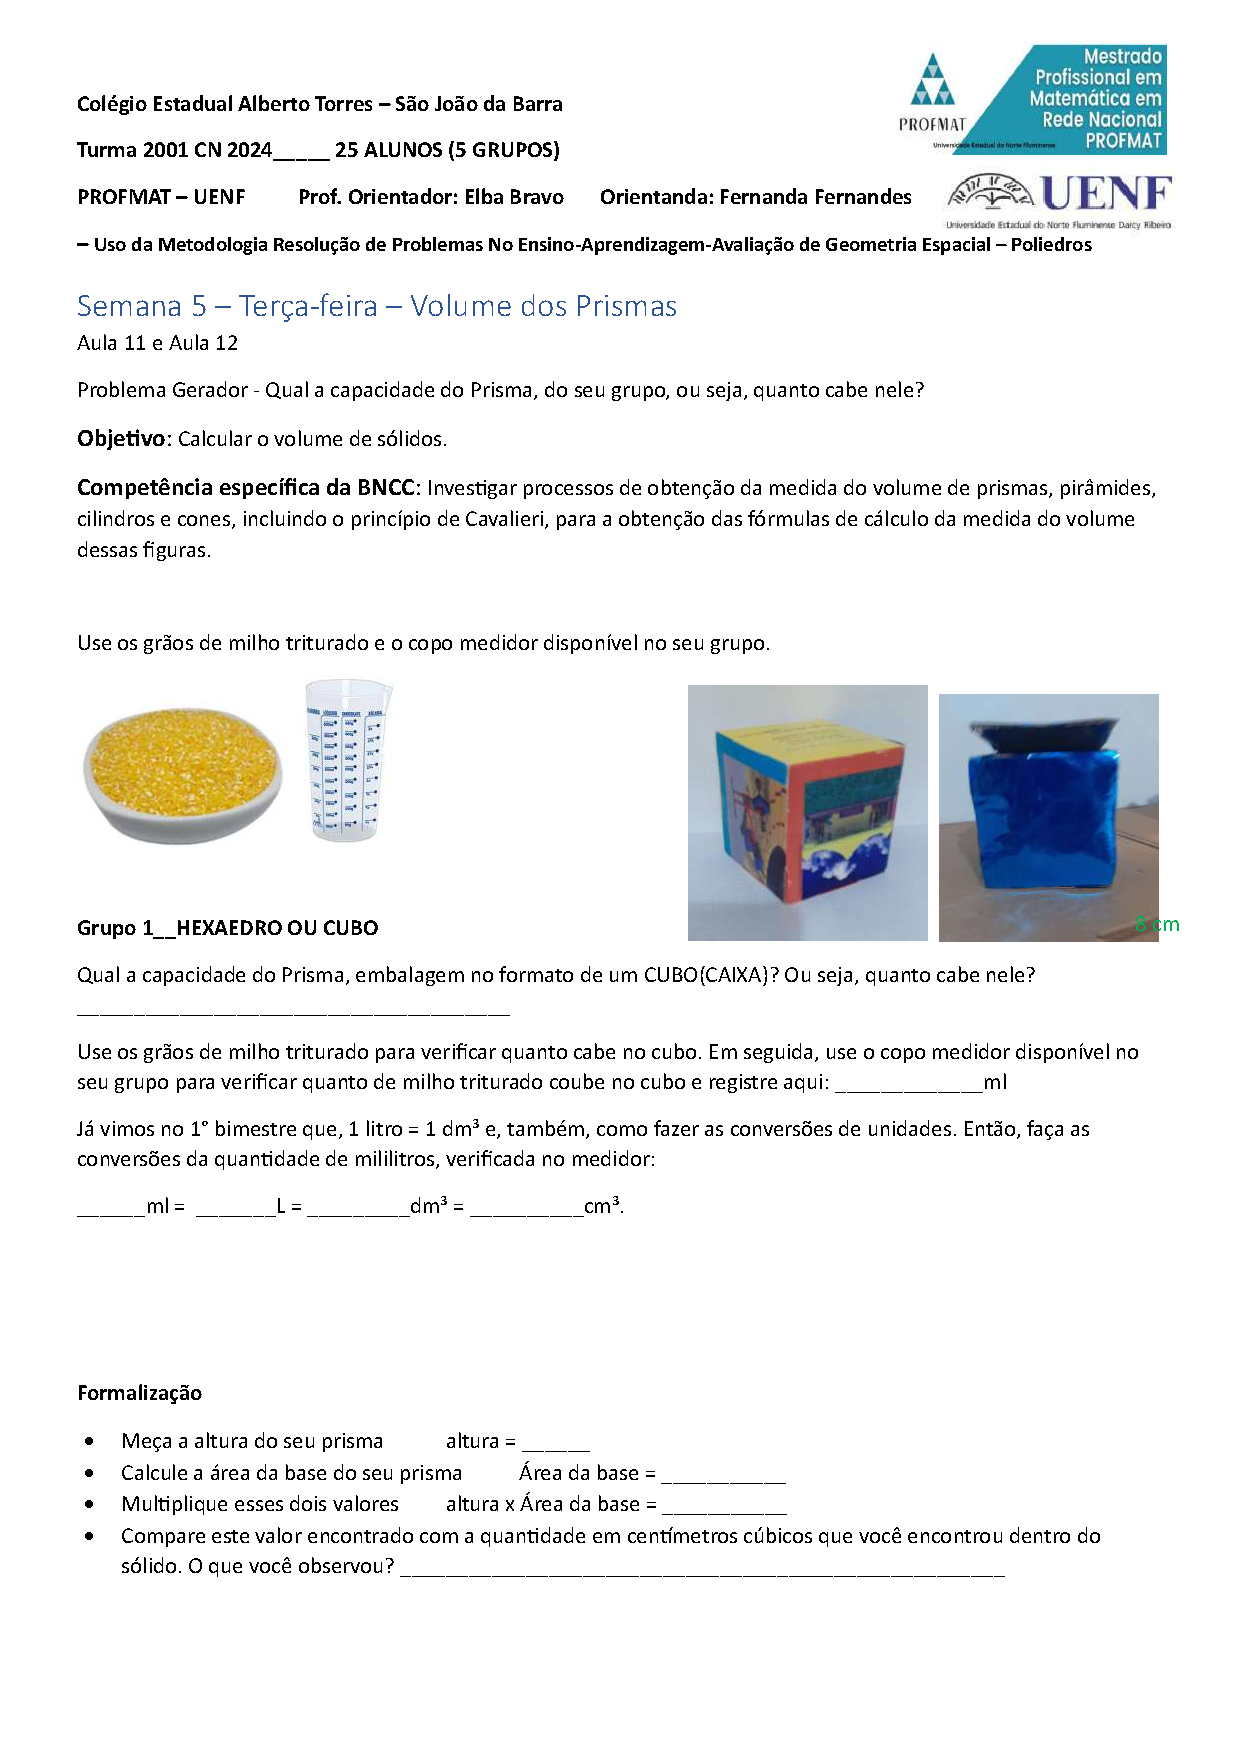
\includepdf[pages=-]{Aulas/pdf11e12_compressed}

    % \chapter{Aulas 13 e 14}
    \label{ApendiceH}
    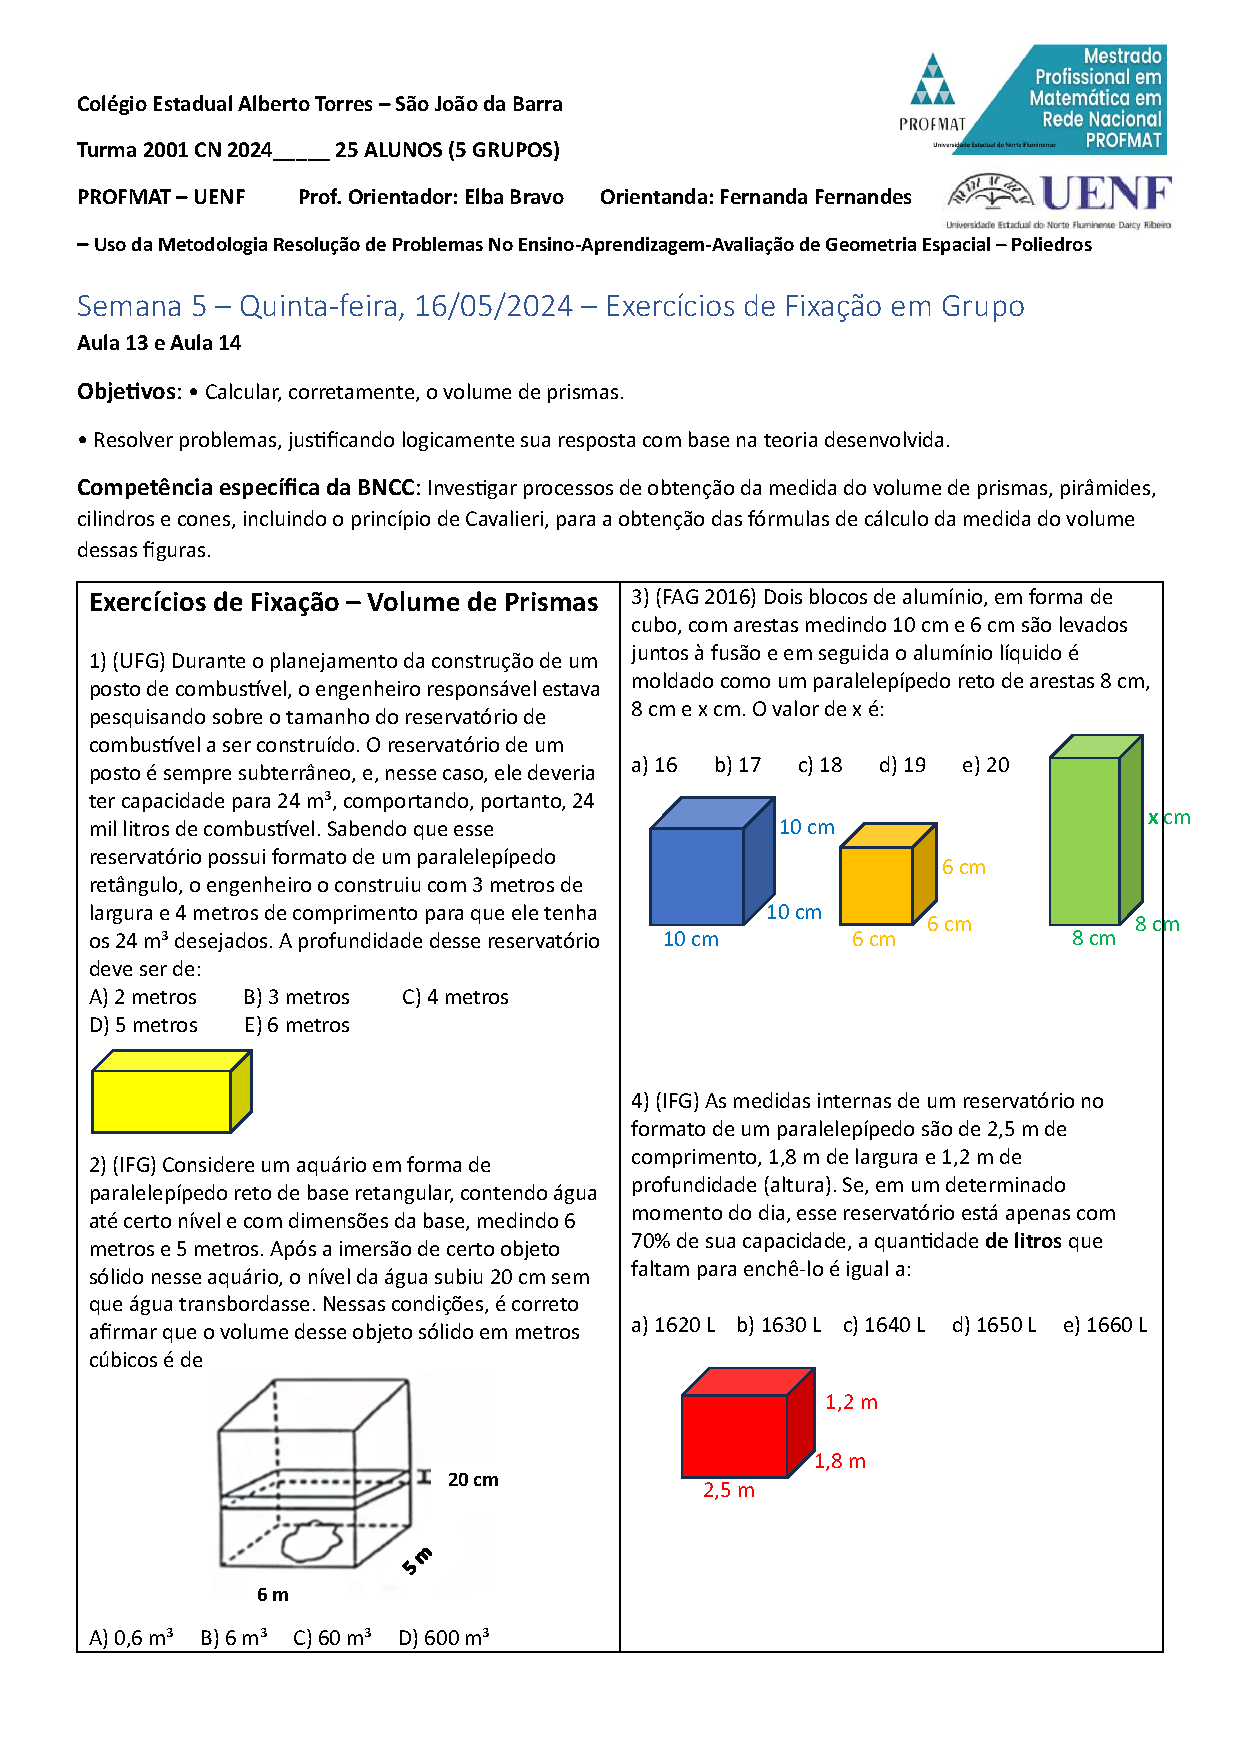
\includepdf[pages=-]{Aulas/pdf13e14}

    % \chapter{Aulas 15 e 16}
    \label{ApendiceI}
    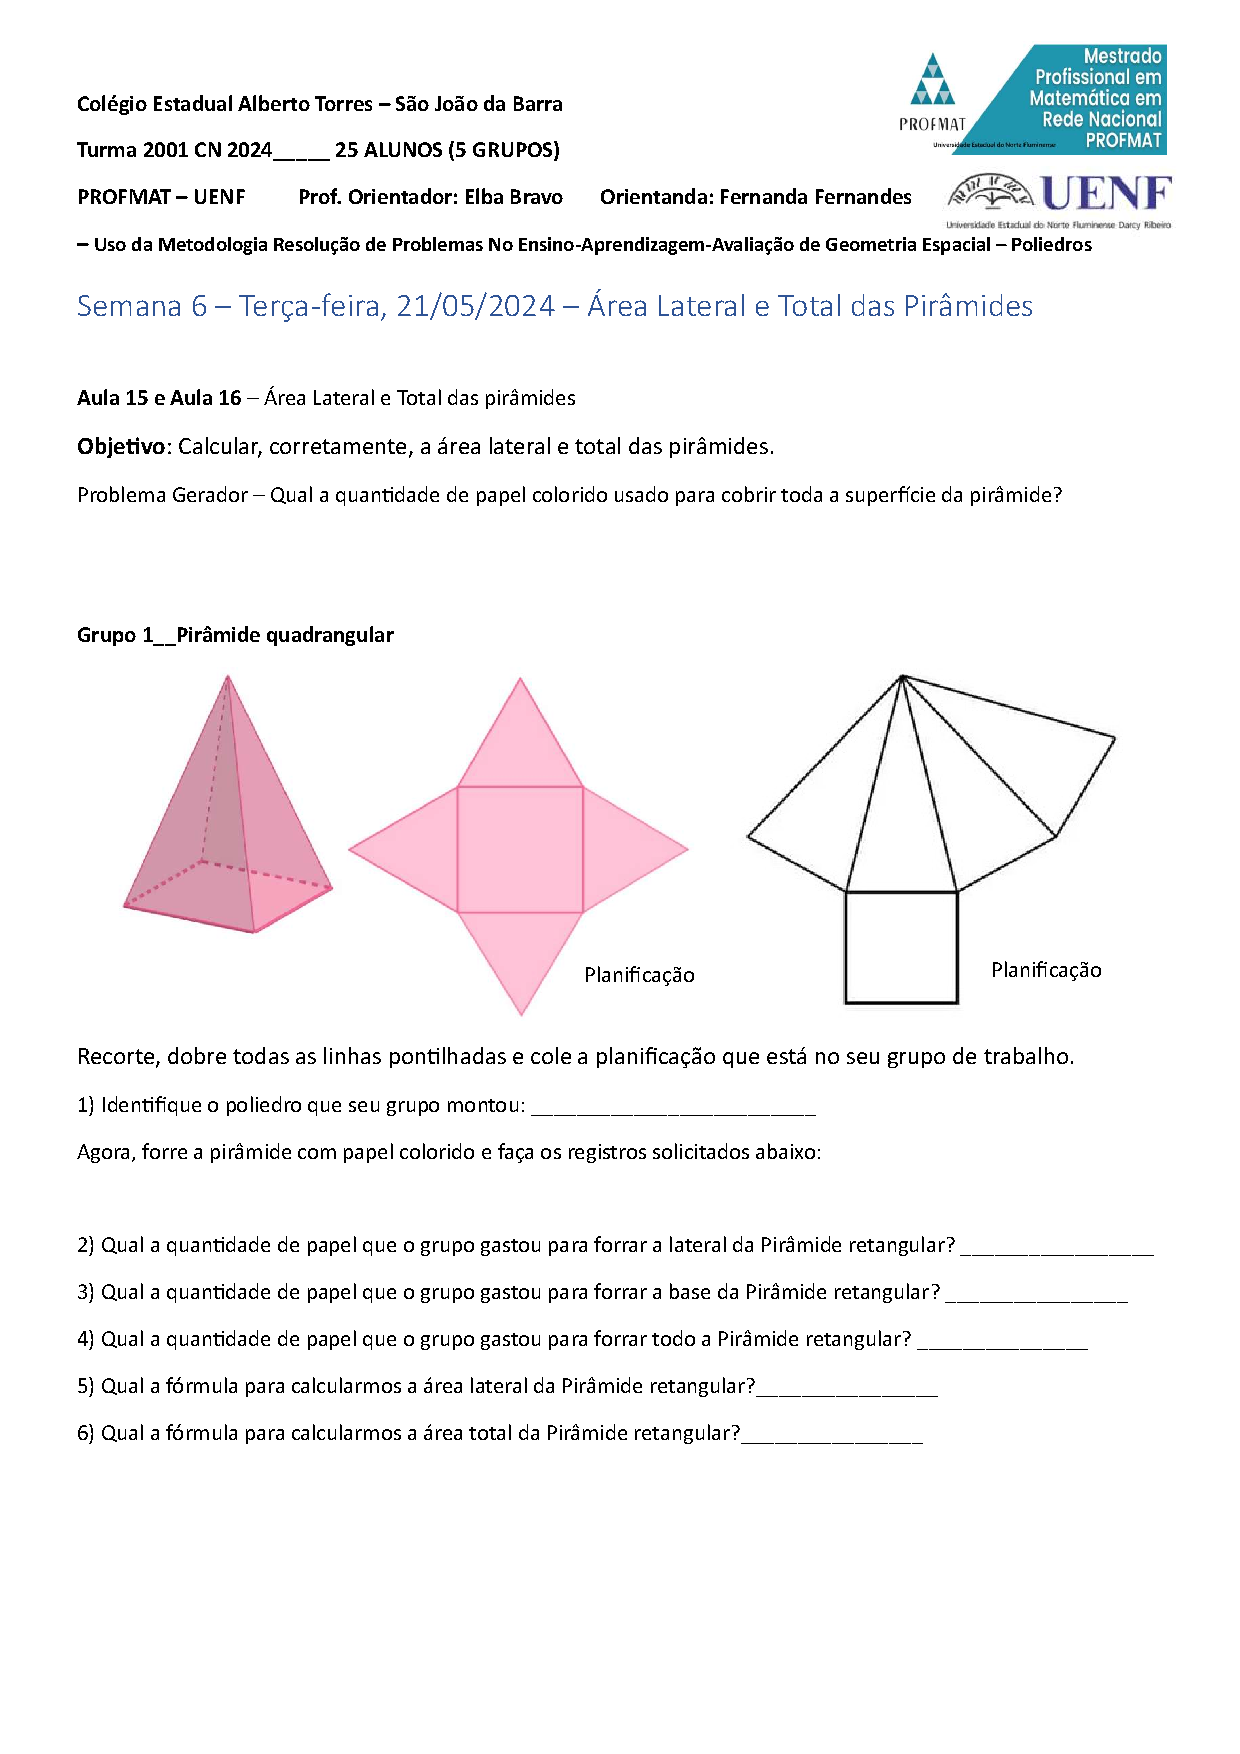
\includepdf[pages={1-5}]{Aulas/pdf15e16}

    % \chapter{Aulas 17 e 18}
    \label{ApendiceJ}
    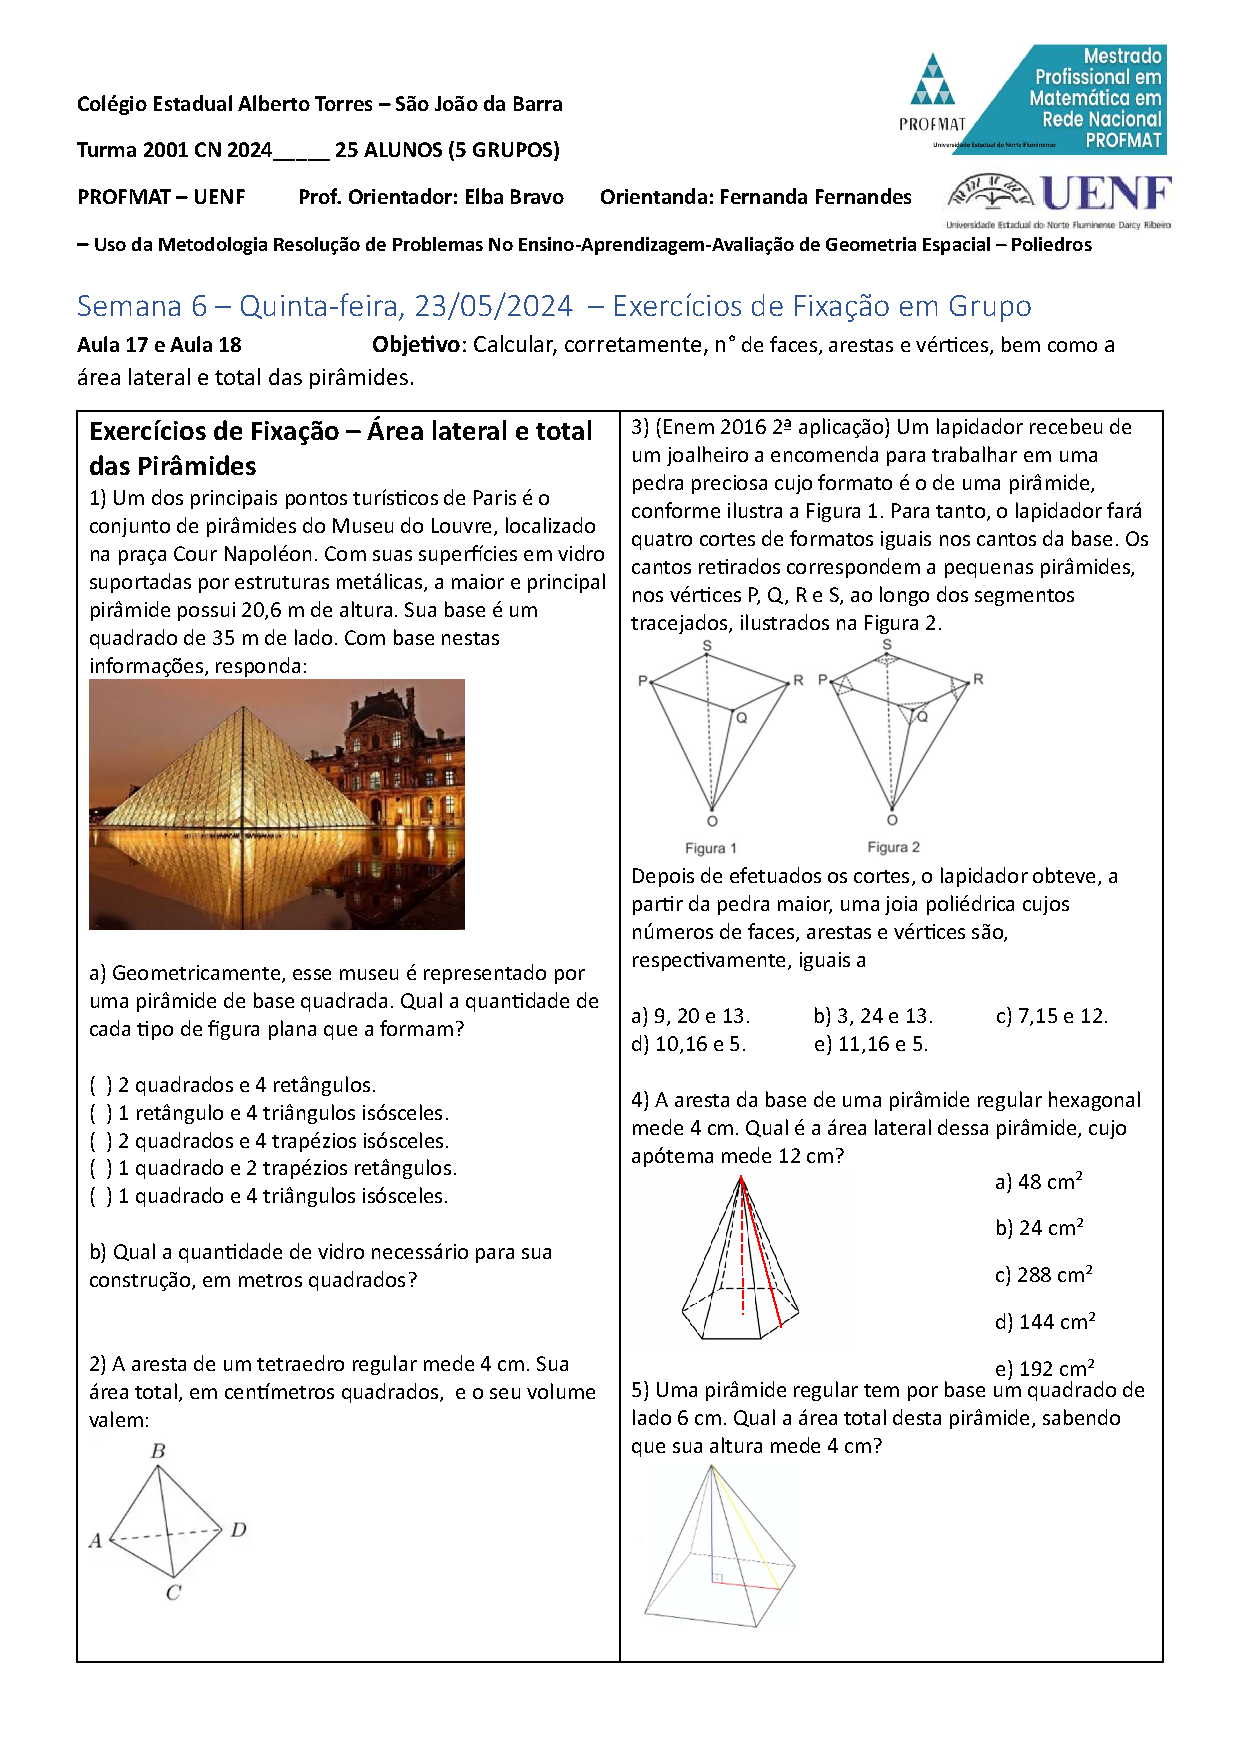
\includepdf[pages=-]{Aulas/pdf17e18}

    % \chapter{Aulas 19 e 20}
    \label{ApendiceK}
    \includepdf[pages=-]{Aulas/pdf19e20}

    % \chapter{Aulas 21 e 22}
    \label{ApendiceL}
    \includepdf[pages=-]{Aulas/pdf21e22}

    % \chapter{Aulas 23 e 24}
    % \label{ApendiceM}
    % \includepdf[pages=-]{Aulas/pdf23e24}

    % \chapter{Aulas 23 e 24}
    \label{ApendiceM}
    \includepdf[pages=-]{Aulas/pdf23e24_compressed}

    %\includepdf{teste} % No apêndice pode ser incluida paginas digitalizadas em qualquer formato como no exemplo abaixo

\end{apendicesenv}


% % ----------------------------------------------------------
% Anexos
% ----------------------------------------------------------

% ---
% Inicia os anexos
% ---
\begin{anexosenv}

	Imprime uma página indicando o início dos anexos
	\partanexos

	---
	\chapter{Título do anexo}
	---
	Colocar aqui os anexos
	---

	----------------------------------------------------------------------
	No anexo pode ser incluida paginas digitalizadas em qualquer formato
	como no exemplo abaixo
	----------------------------------------------------------------------
	\includepdf[pages={1-3}]{Quadros-Tabelas-Figuras.pdf}


\end{anexosenv} % Não usado
% %---------------------------------------------------------------------
% INDICE REMISSIVO
%---------------------------------------------------------------------
\phantompart
\printindex
%---------------------------------------------------------------------
 % Não usado

\end{document}
